\documentclass{article}

\usepackage{url}
\usepackage[hmargin=1.5in]{geometry}
\usepackage{amsmath}
\usepackage{amssymb}
\usepackage{amsthm}
%\usepackage{eqnarray}
\usepackage{stmaryrd} %% needed for mapsto arrows in commutative diagrams
\usepackage{bm} %% for putting series names in bold
%%\usepackage{amsthm}
\usepackage{graphicx}
\usepackage{fancyhdr}
\usepackage{enumitem}
\usepackage[svgnames]{xcolor} %% for revisions
\usepackage{xparse} %% for squiggly underlines
\usepackage{tikz-cd} %% for term norm scratch work
\usepackage{tikz}
%\usepackage{eqnarray}

\let\Re\relax
\DeclareMathOperator{\Re}{Re}
\let\Im\relax
\DeclareMathOperator{\Im}{Im}

\usetikzlibrary{bbox}
\usetikzlibrary{fadings}

\pgfdeclareradialshading{radialedge}{\pgfpointorigin}{%
  color(0bp)=(transparent!0);
  color(20bp)=(transparent!0);
  color(22bp)=(transparent!10);
  color(24bp)=(transparent!90);
  color(25bp)=(transparent!100)
}
\pgfdeclarefading{radial edge}{\pgfuseshading{radialedge}}%

% domains
\newcommand{\dualsector}[2]{\Omega_{#1|#2}}

% function spaces
\newcommand{\cont}{\mathcal{C}}
\newcommand{\holo}{\mathcal{H}}
\newcommand{\singexp}[2]{\mathcal{H}L^\infty_{#1, #2}}
\newcommand{\singexpalg}[1]{\singexp{#1}{\bullet}}
\newcommand{\dualsingexp}[2]{\widehat{\mathcal{H}}L^\infty_{#1, #2}}
\newcommand{\dualsingexpalg}[1]{\dualsingexp{#1}{\bullet}}
\newcommand{\holoL}[1]{\mathcal{H}L^{#1}} %% remove once we stop using old arguments

%% editing
\newcommand{\done}[1]{\textcolor{gray}{#1}}

% convenience aliases
\newcommand{\maps}{\colon}
\newcommand{\acts}{\mathbin{\raisebox{\depth}{\rotatebox{-90}{$\circlearrowright$}}}}

% symbology
\newcommand{\Z}{\mathbb{Z}}
\newcommand{\R}{\mathbb{R}}
\newcommand{\C}{\mathbb{C}}
\newcommand{\Q}{\mathbb{Q}}
\usepackage{tikz}
\usepackage{tikz-cd}
\usepackage{rotating}
\newcommand*{\isoarrow}[1]{\arrow[#1,"\rotatebox{90}{\(\sim\)}"
]}

% regular singular volterra operator
\newcommand{\volterra}{\mathcal{V}}
\newcommand{\hardpart}{\mathcal{V}_0}
\newcommand{\softpart}{\mathcal{V}_\star}
%%\newcommand{\kerwhole}{k}
\newcommand{\hardker}{k_0}
%%\newcommand{\softker}{k_\star}
\newcommand{\solwhole}{f}
\newcommand{\solproto}{f_0}
\newcommand{\solptb}{f_\star}
%%\newcommand{\roots}{\mathfrak{B}}

%% for the figure
% colors
\definecolor{smoked}{RGB}{216, 212, 204}
\definecolor{mauve}{RGB}{200, 55, 171}
\definecolor{apricot}{RGB}{250, 144, 4}
\definecolor{sky}{RGB}{66, 169, 244}
\definecolor{plum}{RGB}{76, 0, 102}

% === phase space laplace ===
\usepackage{etoolbox}

\usetikzlibrary{math, 3d, calligraphy}

% --- styles ---

\definecolor{pwbeige}{RGB}{172, 146, 122}
\definecolor{pworange}{RGB}{245, 153, 30}

\tikzset{
  surf/.style={pwbeige!10},
  leaf/.style={thin, pwbeige!60},
  sing/.style={thick, pworange},
  ray/.style={thick}
}

% --- cotangent fibers ---

\newcommand{\rfiber}{1.5}
\pgfmathsetmacro{\rshade}{1.5*\rfiber}

\newcommand{\drawfiber}{
  \foreach \sgn in {-1, 1} {
    \calligraphy[scale=\sgn, copperplate, heavy, heavy line width=0.25mm]
      (\rfiber, \rfiber) -- (\rfiber, -\rfiber)
      (\rfiber, -\rfiber) -- (-\rfiber, -\rfiber);
  };
}

% set up PGF keys
\pgfkeys{
  /laplace/.cd,
  drop/.store in=\fiberdrop,   drop/.value required,
  shade/.store in=\fibershade, shade/.default=true,
  degree/.store in=\fiberdeg,  degree/.value required,
  phase/.store in=\fiberphase, phase/.value required,
  dis/.store in=\fiberdis,     phase/.value required,
  dual/.store in=\fiberdual,   dual/.default=true
}

\newcommand{\fiberdescender}[1]{
  \calligraphy[copperplate, light, thin] (0, -\rfiber) -- (0, -#1);
}

\newcommand{\fibershading}[2]{
  \tikzmath{
    \shadestart = (-90 - #1) / \fiberdeg;
    \shadeend = (90 - #1) / \fiberdeg;
  }
  \fill[pwbeige!30, draw=pwbeige!60] (0, 0) ++(-#1:#2) -- ++(\shadestart:\rshade) arc (\shadestart:\shadeend:\rshade) -- cycle;
}

\newenvironment{fiber}[1][]{%
  \pgfkeys{/laplace/.cd, drop=0, shade=false, degree=1, phase=0, dis=0, #1}
  \begin{scope}
    \fill[surf] (-\rfiber, -\rfiber) rectangle (\rfiber, \rfiber);
    \clip (-\rfiber, -\rfiber) rectangle (\rfiber, \rfiber);
    \tikzmath{
      if \fibershade then {
        print \fibershading{\fiberphase}{\fiberdis};
      };
    }
}{% ...
  \end{scope}
  % see TikZ docs for branching statements
  % https://tikz.dev/library-math#sec-58.5
  \tikzmath{
    if \fiberdrop > 0 then {
      print \fiberdescender{\fiberdrop};
    };
  }
  \drawfiber
}

\newcommand{\genfibercontent}[1][]{
  \pgfkeys{/laplace/.cd, dual=false, #1}
  \pgfmathsetmacro{\hatch}{\rfiber/8};
  \pgfmathsetmacro{\firsthatch}{-\rfiber+\hatch}
  \pgfmathsetmacro{\nexthatch}{-\rfiber+2*\hatch}
  \pgfmathsetmacro{\hatchstop}{\rfiber-\hatch/2}
  \foreach \y in {\firsthatch, \nexthatch, ..., \hatchstop} {
    \tikzmath{
      coordinate \drawfrom;
      coordinate \drawto;
      if \fiberdual then {
        \drawfrom = (\y, -\rfiber);
        \drawto = (\y, \rfiber);
      } else {
        \drawfrom = (-\rfiber, \y);
        \drawto = (\rfiber, \y);
      };
    }
    \draw[leaf] (\drawfrom) -- (\drawto);
  };
  \fill circle (\dotsize);
}

\newcommand{\singfibercontent}{
  % nonsingular leaves
  \foreach \sector in {30, 90, ..., 330} {
    \tikzmath{
      \farout = 45*floor((\sector + 59) / 45);
      \tfarout = 3*(\farout - \sector);
      \rfarout = \rfiber/sin(45+mod(\farout-45, 90));
    }
    \pgfmathsetmacro{\rmax}{sin(\tfarout) * pow(\rfarout, 3)}
    \foreach \r in {0.5, 1.0, ..., \rmax} {
      \pgfmathsetmacro{\win}{asin(\r/(2*\rmax))}
      \draw[leaf, rotate=\sector, domain=\win:{180-\win}, variable=\t] plot ({\t/3}:{(\r/sin(\t))^(1/3)});
    };
    
    % singular leaves
    \foreach \ang in {90, 210, 330} {
      \draw[sing] (\ang:{-sqrt(2)*\rfiber}) -- (\ang:{sqrt(2)*\rfiber});
    };
    \fill[sing] circle (\dotsize);
  };
}

% --- posititon plane ---

\pgfmathsetmacro{\hatch}{2/3}
\tikzmath{
  \phase = 15;
  \dotsize = 0.04;
  \drop = 3.5;
  \xsing = 2;
  \zsing = 4*\hatch;
  \xgen = 6;
  \zgen = 8*\hatch;
  \rcut = 1/5;
}

\newcommand{\ray}[2]{
  \draw[ray] (#1, #2) -- (8, {#2 + (8-#1)*tan(\phase)});
}

% local picture of the Laplace transform
\newcommand{\basicLaplace}{
\begin{tikzpicture}[scale=0.9]
% position space
\begin{fiber}
  \genfibercontent
  \ray{0}{0}
\end{fiber}
\node[anchor=north, outer sep=1mm, font=\footnotesize]
  at (0, -\rfiber) {position space};

% frequency space
\begin{scope}[shift={(4 + 0.25*8/3, 0)}]
  \begin{fiber}[shade, phase=\phase]
    \genfibercontent[dual]
  \end{fiber}
  \node[anchor=north, outer sep=1mm, font=\footnotesize]
    at (0, -\rfiber) {frequency space};
\end{scope}
\end{tikzpicture}
} % \basicLaplace

% phase space picture of the Laplace transform
\newcommand{\phaseSpaceLaplace}{
\begin{tikzpicture}[z={(0.25cm, 0.2cm)}, scale=0.9]
% position plane
\begin{scope}[canvas is xz plane at y=0]
  % surface
  \fill[surf]
    (0, 0) -- (0, \zsing-\rcut)
    -- ++(\xsing-\rcut, 0) arc (-90:90:\rcut) -- (0, {\zsing + \rcut})
    -- (0, 8) --(8, 8) -- (8, 0) -- cycle;
  
  % hatching
  \pgfmathsetmacro{\nexthatch}{2*\hatch}
  \pgfmathsetmacro{\singstop}{\zsing - \hatch/2}
  \foreach \z in {\hatch, \nexthatch, ..., \singstop} {
    \draw[leaf] (0, \z) -- (8, \z);
  };
  \pgfmathsetmacro{\singstart}{\zsing + \hatch}
  \pgfmathsetmacro{\singnext}{\zsing + 2*\hatch}
  \pgfmathsetmacro{\hatchstop}{8 - \hatch/2}
  \foreach \z in {\singstart, \singnext, ..., \hatchstop} {
    \draw[leaf] (0, \z) -- (8, \z);
  };
  
  % singular leaves
  \begin{scope}[sing]
    \draw (\xsing, \zsing) -- (8, \zsing);
    \draw (0, \zsing-\rcut) -- ++(\xsing-\rcut, 0) arc (-90:90:\rcut) -- (0, {\zsing + \rcut});
  \end{scope}
  
  % integration rays
  \ray{\xgen}{\zgen}
  \ray{\xsing}{\zsing}
  
  % outline
  \calligraphy[copperplate, heavy, heavy line width=0.25mm]
    (0, 0) -- (0, \zsing-\rcut)
    (0, \zsing+\rcut) -- (0, 8)
    (0, 8) -- (8, 8)
    (8, 8) -- (8, 0)
    (8, 0) -- (0, 0);
\end{scope}

% generic fiber
\begin{scope}[canvas is xy plane at z=\zgen, shift={(\xgen, \drop)}]
  \begin{fiber}[drop=\drop, shade, phase=\phase]
    \genfibercontent[dual]
  \end{fiber}
\end{scope}

% singular fiber
\begin{scope}[canvas is xy plane at z=\zsing, shift={(\xsing, \drop)}]
  \begin{fiber}[drop=\drop, shade, degree=3, phase=\phase]
    \singfibercontent
  \end{fiber}
\end{scope}

% generic point
\fill (\xgen, 0, \zgen) circle (\dotsize);

% singular point
\fill[sing] (\xsing, 0, \zsing) circle (\dotsize);

% labels
\begin{scope}[overlay]
  \node (surf label) at (9, 0, 4) {$B$};
  \path (surf label) ++(0, \drop, 0) node {$T^*B$};
  \node[outer sep=0.15mm, font=\footnotesize, align=left]
    (cut label) at (-1.25, 1.2, \zsing) {branch cut \\ at conical \\ singularity};
  \draw[->] (cut label) to[out=-75, in=180] (-0.25, 0, \zsing);
\end{scope}
\end{tikzpicture}
} % \phaseSpaceLaplace


\newcommand{\series}[1]{\tilde{#1}}
\newcommand{\fracderiv}[3]{\partial^{#1}_{#2, #3}}
\newcommand{\blankbox}{{\fboxsep 0pt \colorbox{lightgray}{\phantom{$h$}}}}
\newcommand{\laplacepde}{\mathcal{D}}
\newcommand{\van}{\mathfrak{m}}
\DeclareMathOperator{\Ai}{Ai}
\usetikzlibrary{matrix,shapes,arrows,decorations.pathmorphing}
\tikzset{commutative diagrams/arrow style=math font}
\tikzset{commutative diagrams/.cd,
mysymbol/.style={start anchor=center,end anchor=center,draw=none}}
\newcommand\MySymb[2][\square]{%
  \arrow[mysymbol]{#2}[description]{#1}}
\tikzset{
shift up/.style={
to path={([yshift=#1]\tikztostart.east) -- ([yshift=#1]\tikztotarget.west) \tikztonodes}
}
}
\DeclareMathAlphabet{\mathpzc}{OT1}{pzc}{m}{it}

\newcommand*{\defeq}{\mathrel{\vcenter{\baselineskip0.5ex \lineskiplimit0pt
                     \hbox{\scriptsize.}\hbox{\scriptsize.}}}%
                     =}
\newcommand*{\defeqin}{\mathrel{\vcenter{\lineskiplimit0pt\baselineskip0.5ex
                     \hbox{\scriptsize.}\hbox{\scriptsize.}}}%
                     =}                     

%%\let\Re\relax
%%\DeclareMathOperator{\Re}{Re}

\newcommand{\laplace}{\mathcal{L}}
\newcommand{\borel}{\mathcal{B}}
\newcommand{\aexp}{\text{\ae}}
\newcommand{\deriv}[3]{\partial^{#1}_{#2 \text{ from } #3}}

% theorem environments
\theoremstyle{definition}
\newtheorem{defn}{Definition}
\newtheorem{definition}{Definition}[section]
\newtheorem{remark}[definition]{Remark}
\theoremstyle{plain}
\newtheorem{theorem}{Theorem}[section]
\newtheorem{prop}[definition]{Proposition}
\newtheorem{corollary}[theorem]{Corollary}
\newtheorem{lemma}[definition]{Lemma}
%\newtheorem{conjecture}[definition]{Conjecture}
\newtheorem{claim}[definition]{Claim}
%\newtheorem{exercise}[definition]{Exercise}
\newtheorem*{notation*}{Notation}

% drafting environments
\newenvironment{verify}{\color{ForestGreen}}{\color{black}}
\newenvironment{brainstorm}{\color{violet}\begin{itemize}}{\end{itemize}\color{black}}

% colors
\definecolor{ietocean}{RGB}{0, 30, 140}
\definecolor{ietcoast}{RGB}{0, 150, 173}
\definecolor{ietlagoon}{RGB}{0, 216, 180}

% pretty prince hyperref must always be the last thing in the preamble, always
\usepackage{hyperref}
\hypersetup{
  colorlinks,
  linkcolor={ietcoast},
  citecolor={ietcoast},
  urlcolor={ietcoast}
}

\setcounter{tocdepth}{2}

\title{Borel regularity for ODEs and Thimble Integrals}
\author{Veronica Fantini and Aaron Fenyes}

\begin{document}
\maketitle

\begin{abstract}
    ...
\end{abstract}
\tableofcontents

\begin{brainstorm}
    \item Section~\ref{borel_reg-ODE} and maybe other subsections--revise the proof of the main result for ODE taking into account the results in our paper
    \item Do flagged revisions in Section~\ref{borel-reg-thimble}
    \item Section~\ref{contour-argument-AL}---revise the general contour argument
    \item Revise Section 2, using the formalism of $\singexp{\sigma}{\Lambda}(\Omega)$
    \begin{itemize}
    \item Replace formalism in Section~\ref{sec:reg-decay}
    \end{itemize}
    \item Check which examples are still in the framework of our theorem
    \begin{itemize}
    \item Start a storage document for shelved examples
    \end{itemize}
    \item Section~\ref{resurgence-AL}---Draw intersection points figure
    \item Section~\ref{sec:mod-bessel-lift}---pin down contour
    \item Explain contour figure in Airy example (explain what the regions indicate and what the color)
    \begin{itemize}
    \item Figure out how to release source code. How much do we need to clean it up? Is it okay that it relies on Shadertoy?
    \end{itemize}
    \item Look at ``Plan of the paper'' appendix and confirm that we've included everything we want
    \begin{itemize}
    \item Put future goals in storage document
    \end{itemize}
    \item Veronica doesn't like $\gamma_z$ as notation for Hankel contour. I'll suggest $\mathcal{H}_{1,z}$ where $1$ is the point where the path is centered. 
\end{brainstorm}

\section{Introduction}
\subsection{The unreasonable effectiveness of Borel summation}\label{intro:summation}
%%\subsection{A familiar process: Borel summation}\label{intro:summation}
You can often find a formal power series %\textcolor{magenta}{[double-check that this matches the $\tau$ from the position domain]}
\[ \series{\Phi} = \frac{c_0}{z^\tau} + \frac{c_1}{z^{\tau+1}} + \frac{c_2}{z^{\tau+2}} + \frac{c_3}{z^{\tau+3}} + \ldots, \]
with $\tau \in (0, 1]$, that looks or acts like a solution to a problem whose actual solutions are holomorphic functions of $z$. For example, if you want to understand how the solutions of the holomorphic ordinary differential equation (ODE)
\begin{equation}
\left[ \big[ \big(\tfrac{\partial}{\partial z}\big)^2 - 1 \big] + z^{-1} \tfrac{\partial}{\partial z} - \big(\tfrac{1}{3}\big)^2 z^{-2} \right] \Phi= 0. \label{eqn:bessel-rescaled-1}
\end{equation}
behave near $z = \infty$, you might start by looking for formal {\em transmonomial} solutions $e^{-\alpha z}\,\series{\Phi}$, where $\series{\Phi}$ is a formal power series of the kind above. Setting $\alpha = -1$ and $\tau = \tfrac{1}{2}$ gives a well-behaved recurrence relation for $\series{\Phi}$, which produces the solution 
\begin{equation}
e^{z} \left[ \frac{(-1)!!}{z^{1/2}} + \frac{5}{72} \cdot \frac{1!!}{z^{3/2}} + \frac{385}{31104} \cdot \frac{3!!}{z^{5/2}} + \frac{17017}{6718464} \cdot \frac{5!!}{z^{7/2}} + \ldots \right] \label{series:bessel-ex}
\end{equation}
and its constant multiples (see \cite[equation 10.40.1]{dlmf}). As another example, you might rewrite the integral

\[ \Phi(z) = \int_{\Lambda} \exp\left[-z \left(4 u^3 - 3 u\right)\right]\,du \]
as
\[ e^{z}\, \frac{1}{2\sqrt{3}}\, \int_{-\infty}^\infty e^{-z t^2/2} \left[ 1 - \frac{\sqrt{3}}{9} t + \frac{5}{72} t^2 - \frac{4\sqrt{3}}{243} t^3 + \frac{385}{31104} t^4 - \frac{7\sqrt{3}}{2187} t^5 + \frac{17017}{6718464} t^6 - \ldots \right] dt \]
using the substitution $\tfrac{1}{2} t^2 = 4 u^3 - 3 u + 1$. Na\"{i}vely integrating term by term, you again get the transmonomial~\eqref{series:bessel-ex}---up to a constant.\begin{verify}
    see Mathematica document.
\end{verify}

Once you have the formal solution $\series{\Phi}$, you might try to get an actual solution by applying {\em Borel summation}, which turns a formal power series into a function asymptotic to it. Borel summation works in three steps.
\begin{enumerate}
\item Thinking of $z$ as a ``frequency variable,'' we take the Borel transform (also known as formal inverse Laplace transform) of $\series{\Phi}$, producing a formal power series $\series{\phi}$ in a new ``position variable'' $\zeta$.
\item If $\series{\phi}$ has a positive radius of convergence we say $\series{\Phi}$ is {\em $1$-Gevrey}. We sum $\series{\phi}$ to get a holomorphic function $\hat{\phi}$ on a neighborhood of $\zeta = 0$. Then, by analytic continuation, we expand the domain of $\hat{\phi}$ to a Riemann surface $B$ with a distinguished 1-form $\lambda$---the continuation of $d\zeta$. %\textcolor{orange}{[Nikita has a complementary picture where the Borel plane is the cotangent fiber? Ask more about this.]}
\item Furthermore, if $\hat{\phi}$ grows slowly enough along an infinite ray $b + e^{i\theta}[0, \infty)$ \textcolor{magenta}{[change, explain, or link to notation]} its Laplace transform $\laplace_b^\theta \hat{\phi}$ (see Section \ref{laplace:ordinary}) turns out to be a holomorphic function of $z$, well-defined on some sector of the frequency plane. In this case, we say $\tilde{\Phi}$ is {\em Borel-summable}, and we call $\hat{\Phi}:=\laplace_b^\theta \hat{\phi}$ its {\em Borel sum} at $b$. 
\end{enumerate}
The series $\series{\Phi}$ and its Borel sum $\hat{\Phi}$ have a special relationship, which is best described in the language of {\em Gevrey asymptoticity}. %\textcolor{magenta}{[Do we need to extend these definitions, and the associated theorems, to cover slight series? Hopefully it wouldn't be too hard, but it would be a pain.]}
\begin{defn}
On an open, possibly bounded sector $\Omega$ around $\infty$, a power series
\begin{equation}\label{series:asymp-defn}
\frac{a_1}{z} + \frac{a_2}{z^2} + \frac{a_3}{z^3} + \frac{a_4}{z^4} + \ldots
\end{equation}
is {\em asymptotic} to a holomorphic function $F$ if
\[ \left|F - \left(\frac{a_1}{z} + \frac{a_2}{z^2} + \ldots + \frac{a_n}{z^n} \right) \right| \in o_{z \to \infty}\big(|z|^{-n}\big) \]
over all orders $n$. We'll use the symbol $\sim$ to denote the asymptotic of $F$, namely we'll write \[F\sim \sum_{n\geq 1} a_n z^{-n}.\]
\end{defn}
If two power series of the form \eqref{series:asymp-defn} are asymptotic to the same function, they must be equal; this can be deduced from the triangle inequality. The power series which is asymptotic to a given function on a given open sector, if it exists, is therefore an intrinsic property of the function: it's the function's {\em asymptotic expansion} on that sector. The functions that have asymptotic expansions on a given sector form a ring~\cite[Section~A.4]{nikolaev2023existence}, and the map that sends such a function to its asymptotic expansion is a ring homomorphism. We'll denote such map with the symbol $\aexp$. More generally, when the asymptotic expansion is taken in the direction $\theta$ at infinity, i.e. as $z\to e^{i\theta}\infty$, we'll write $\aexp^\theta$.  

\begin{defn}
\textcolor{orange}{[Define $\aexp^\theta$ homomorphism that sends a function with an asymptotic expansion on a sector that contains the $\theta$-ray to its asymptotic expansion on that sector.\ldots]}
\end{defn}
\textcolor{RoyalBlue}{The {\em asymptotic expansion} map $\aexp^\theta$ sends a holomorphic function that vanishes at $\infty$ to the unique power series of the form \eqref{series:asymp-defn} which is asymptotic to it on the half-plane $\Re e^{i\theta}z > 0$ (see \cite[Theorem~C.11]{nikolaev2023existence}).}

\textcolor{orange}{[State theorem: differentiation commutes with $\aexp^\theta$ under certain circumstances. See Erdelyi's {\em Asymptotic Expansions}, \S 1.6. For basic facts about uniform asymptoticity, see \S 5.7.2 of Mitschi and Sauzin. Theorem~5.20 and its rephrasing say that the Laplace transform of a function is uniformly asymptotic to the formal Laplace transform of the function's Taylor series.]}

\begin{defn}\label{def:unif-gevrey-asymp}
On an open sector $\Omega$ around $\infty$, a power series of the form \eqref{series:asymp-defn} is {\em uniformly $1$-Gevrey asymptotic} to a holomorphic function $F$ if there's a constant $A \in (0, \infty)$ for which
\[ \left|F - \left(\frac{a_1}{z} + \frac{a_2}{z^2} + \ldots + \frac{a_{n-1}}{z^{n-1}} \right) \right| \lesssim \frac{A^n n!}{|z|^n} \]
over all orders $n$ and all $z \in \Omega$. We'll use $\lesssim$ throughout the paper to mean ``bounded by a constant multiple of,'' with the same constant over all the specified variables.
\end{defn}
To compare the Borel sum $\hat{\Phi}$ with the original series $\series{\Phi}$, let's take it one more step, sending it back into the world of formal power series by taking its asymptotic expansion.

\begin{enumerate}[start=4]
\item By construction, $\aexp^\theta \hat{\Phi} = \series{\Phi}$. It turns out that $\hat{\Phi}$ is not only asymptotic to $\series{\Phi}$, but {\em {uniformly} $1$-Gevrey}-asymptotic~\cite[Corollary~5.23]{diverg-resurg-i}.
\end{enumerate}

The Borel summation process is summarized in the following diagram:
\begin{center}
\begin{tikzcd}
& \text{problem} & \\
\hat{\Phi} \arrow[ru, dotted, no head, tail] \arrow[rr, mapsto, "\aexp^\theta", "\text{($1$-Gevrey)}"'] & & \series{\Phi} \arrow[lu, no head, tail, "\parbox{10mm}{\centering\scriptsize formally solves}"'] \arrow[dd, mapsto, "\borel"] \\
& & \\
\hat{\phi} \arrow[uu, mapsto, "\laplace_b^\theta"] & & \tilde{\phi} \arrow[ll, mapsto, "\text{sum}"] 
\end{tikzcd}
\end{center}

You can't be sure {\em a priori} that $\hat{\Phi}$ solves your original problem, even if you know that $\series{\Phi}$ is asymptotic to an actual solution. After all, $\series{\Phi}$ is asymptotic to lots of functions; Borel summation just picks one of them. In many cases, however, Borel summation picks correctly, delivering an actual solution to your problem. The question of how that happens is the starting point for this paper.

%\color{gray}
%\begin{itemize}
%\item \done{You can often find a formal power series $\tilde{\Phi} = \ldots$ that looks or acts like a solution to a problem whose actual solutions are holomorphic functions of $z$. For example\ldots}
%\begin{itemize}
%\item \done{Exponential integral: na\"{i}ve saddle point expansion.}
%\item \done{ODE: formal solution.} Existence theorem in \cite{diverg-resurg-iii}?
%\item Feynman diagram series?
%\end{itemize}
%\item Once you have $\tilde{\Phi}$, you might try applying {\em Borel summation}, which turns a formal power series into a function asymptotic to it.
%\begin{itemize}
%\item \done{Borel summation work in three steps. First we turn the formal power series $\tilde{\Phi}$ \textcolor{magenta}{[$\tilde{\Phi}(z)$]} in the ``frequency variable'' $z$ into a formal power series $\tilde{\phi}$ in a new ``position variable'' $\zeta$.}
%\item \done{The series $\tilde{\phi}$ turns out to have a \textcolor{magenta}{[finite]} positive radius of convergence, so it defines a holomorphic function $\hat{\phi}$. By analytic continuation, we can expand the domain of $\hat{\phi}$ to a Riemann surface $B$ with a distinguished 1-form $\lambda$---the continuation of $d\zeta$.}
%\item \done{If $\hat{\phi}$ grows slowly enough along an infinite ray $\Gamma_b^\theta := b + e^{i\theta}[0, \infty)$ \textcolor{magenta}{[decide notation]}, its Laplace transform $\laplace_b^\theta \hat{\phi} := \ldots$ is a holomorphic function of $z$, well-defined on some sector of the frequency plane. In this case, we say $\tilde{\Phi}$ is {\em Borel-summable}, and we call $\laplace_b^\theta \hat{\phi}$ its {\em Borel sum} at $b$.}
%\item {[Draw the square!]}
%\end{itemize}
%\item Different functions can be asymptotic to the same power series, and Borel summation picks one of them.
%\item In many cases, it picks correctly, producing an actual solution to your problem.
%\begin{itemize}
%\item The question of how that happens is the starting point for this paper.
%\item (In both of the cases that we study, the Borel sum of $\tilde{\Phi}$ is always taken at a zero of $\lambda$, rather than an arbitrary point in $B$. For ODEs, our treatment explains why the zeroes of $\lambda$ play a special role.)
%\end{itemize}
%\end{itemize}
%\color{black}
\subsection{A new perspective: Borel regularity}
\subsubsection{Introducing Borel regularity}
We consider an holomoprhic function $\Phi$, solution of our problem. Taking its asymptotic expansion along the half-plane $\Re e^{i\theta}z > 0$, we get a formal power series $\series{\Phi}$. 

%\textcolor{Tan}{We consider a new diagram: we start reading it from the upper-left corner, namely we assume there exists a holomorphic function $\Phi$ which is asymptotic to a formal power series $\series{\Phi}$ as $\Re e^{i\theta}z$ goes to $\infty$ in the direction of $\theta$}

\begin{center}
\begin{tikzcd}
& \text{problem} & \\
\Phi \arrow[ru, no head, tail, swap, "\text{solves}"' ] \arrow[rrd, mapsto, "\aexp^{\theta}"]& & \\
\hat{\Phi} \arrow[rr, "\aexp^{\theta}", "\text{($1$-Gevrey)}"'] & & \series{\Phi} \arrow[luu, no head, tail, swap, "\parbox{10mm}{\centering\scriptsize formally solves}"] \arrow[dd, mapsto, "\borel"] \\
& & \\
\hat{\phi} \arrow[uu, mapsto, "\laplace_b^\theta"] & & \series{\phi} \arrow[ll, mapsto, "\text{sum}"] 
\end{tikzcd}
\end{center}
If $\series{\Phi}$ is Borel-summable, as described in Section~\ref{intro:summation}, its Borel sum $\hat{\Phi}$ is a new holomorphic function.
Since different functions can be asymptotic to the same power series, taking the Borel sum of the asymptotic series of $\Phi$ must smooth away some details. We'll therefore call this process {\em Borel regularization}. Explicitly, Borel regularization works in four steps.
\begin{enumerate}
\item Take the asymptotic expansion $\series{\Phi} = \aexp^{-\theta} \Phi$.
\item Take the Borel transform $\series{\phi} = \borel \series{\Phi}$.
\item Take the sum $\hat{\phi}$ of $\series{\phi}$, and expand its domain to a Riemann surface with a distinguished $1$-form, as before.%\textcolor{red}{This is possible, by definition, if $\series{\Phi}$ is $1$-Gevrey.[Veronica: I'll remove this! Being Gevrey implies that the Borel transform is convergent, not that we can analytically continue it]}
\item Take the Laplace transform $\hat{\Phi} = \laplace_{\zeta, 0}^\theta \hat{\phi}$. This is possible, by definition, if $\series{\Phi}$ is Borel-summable.\footnote{More generally, we're allowed to take the Laplace transform at another point $b \in B$. This would be natural in our study of ODEs and thimble integrals.}
\end{enumerate}
We'll say a function is {\em Borel-regularizable} if its asymptotic expansion is Borel-summable, ensuring that we can carry out the last two steps.

Defining a regularization process picks out a class of regular functions: the ones that are invariant under regularization. We'll say a function is {\em Borel regular} if it's Borel-regularizable and Borel regularization leaves it unchanged. In other words, $\Phi$ is Borel regular if $\hat{\Phi} = \Phi$.

\subsubsection{Borel regularity sometimes explains why Borel summation works}\label{borel-reg:explanatory-power}
The idea of Borel regularity can help us understand why Borel summation is so effective in some situations. Roughly speaking, Borel summation works well for problems that admit solutions in terms of Laplace transform. 

The central goal of this paper is to explain, from this perspective, why Borel summation works well for the two kinds of problems exemplified in Section~\ref{intro:summation}.
\begin{enumerate}
\item Solving a linear ODE of single level~$1$ \cite[Section 2.1]{EcalleIII}\cite[Section~5.2.2.1]{diverg-resurg-iii}. One example is Equation~\eqref{eqn:bessel-rescaled-1}. \textcolor{magenta}{The general example [not anymore---we've restricted]} is the equation $\mathcal{P} \Phi = 0$ given by a differential operator of the form
\[ \mathcal{P} = P(\partial_z) + \frac{1}{z} Q(\partial_z) + \frac{1}{z^2} R(z^{-1}), \]
where $P$ is a monic degree-$d$ polynomial, $Q$ is a degree-$(d-1)$ polynomial that's non-zero at every root of $P$, and $R(z^{-1})$ is holomorphic in some disk $|z| > A$ around $z = \infty$. We'll restrict our attention to the case where the roots of $P$ are simple (see Section \ref{borel_reg-ODE}).

The form of $\mathcal{P}$ derives from Equation~2.2.3 of \cite[pag. 105]{EcalleIII}, which encompasses both linear and nonlinear ODEs of level $1$. Borel summation is more involved for the nonlinear ones, raising the question of whether our analysis generalizes.
%
\item Evaluating a certain kind of integral: a one-dimensional {\em thimble integral}
%
\begin{equation*}
I(z)\defeq\int_{\Lambda}\exp\big[-z f\big] \nu
\end{equation*}
where $f\colon X\to \mathbb{C}$ is a holomorphic functions with isolated and non-degenerate critical points, $X$ is $1$-dimensional complex manifold, $\nu\in\Omega^1(X)$ is holomorphic $1$-form in $X$ and $\Lambda$ is a suitable contour such that $I(z)$ is a holomorphic function of $z$.  
\end{enumerate}
These two problems are closely linked. By playing with derivatives of an exponential integral, you can often find a linear ODE that the integral satisfies. Conversely, for many classical ODEs, there are useful bases of exponential integral solutions.

%Notice that our starting point is quite different: we assume $\Phi$ is a holomorphic functions such that it is either a thimble integral or it solves an ODE with irregular singularity at $\infty$. Then we prove $\Phi$ is Borel regular and in both cases, our proves follow the heuristic of the diagram above. We’ll give precise statements in the following section.

       



%%\item {\em A priori}, we should expect $\hat{\Phi}$ to be different from $\Phi$, because we lose information in passing from $\Phi$ to its asymptotic series.
%%\item Taking the Borel sum of the asymptotic series of $\Phi$ is a regularization process, because it smooths away some perturbations---the ones that are asymptotic to zero along the given ray. We'll call it {\em Borel regularization}.
%%\item Taking the Borel sum of the asymptotic series of $\Phi$ can be seen as a regularization process, because taking asymptotics erases information. We'll call this process {\em Borel regularization}.
%\begin{itemize}
%\item We'll say $\Phi$ is {\em Borel-regularizable} if it's asymptotic to a Borel-summable power series.
%\item We'll say $\Phi$ is {\em Borel regular} if it's Borel-regularizable and Borel regularization leaves it unchanged.
%\item We have the following vector space inclusions:
%\[ \text{Borel regular functions} \subset \text{Borel-regularizable functions} \subset \text{holomorphic functions}. \]
%\item Borel regular functions have been characterized in the literature before; Watson showed a century ago \textcolor{orange}{[Watson]} that a function $\Phi$ is Borel regular whenever there's a constant $c \in (0, \infty)$ with
%\[ |\Phi(z)-\sum_{k=0}^Nc_kz^{-k}| \le c^{N+1} N!|z|^{-N} \]
%over all orders $N$ and all $z$ in a wide enough wedge around infinity. 
%
%Nevanlinna's improvement of Watson's theorem (Sokal, ``An improvement of Watson's theorem on Borel summability'') tells us that for a function $\Phi$ with a well-defined inverse Laplace transform $\phi$, the following conditions are equivalent \textcolor{magenta}{[double check]}:
%\begin{itemize}
%\item $\Phi$ is Borel regular.
%\item $\Phi$ is approximated well, in a certain sense (a weak version of being ``Gevrey-asymptotic''), by its asymptotic series.
%\item $\phi$ grows at most exponentially along the Laplace transform ray.
%\end{itemize}
%\item When its domain is restricted to the space of Gevrey power series, Borel summation is invertible. \textcolor{magenta}{[Need to find a good reference for this, because a small change in the statement would mess up our conclusion. Does \texttt{arXiv:2112.08792}, \S A.2 have the statement we want?]} Thus, Borel regularization acts as a projection operator on the space of Borel-regularizable functions.\textcolor{orange}{[Veronica: Do you mean that if $\Phi\sim\tilde{\Phi}$ and $\tilde{\Phi}$ is Gevrey and Borel summable, then $\Phi=\laplace\circ\borel\tilde{\Phi}$ (i.e. it is Borel regular)? P.Ramis proved that if $\Phi$ is Gevrey asymptotic to $\tilde{\Phi}$, then $\tilde{\Phi}$ is of Gevrey type. In addition, every Gevrey type series $\tilde{\Phi}$ is the Gevrey asymptotics of a holomorphic function. When it is defined, the Borel sum of $\tilde{\Phi}$ is the natural holomorphic function asymptotic to $\tilde{\Phi}$.]}
%\item Borel regularity can help explain why Borel summation is so effective at solving certain kinds of problems, like the ones in Section~\ref{intro:summation}.
%\item The formal solutions of a problem are typically supposed to generalize the actual solutions, in the sense that they include the asymptotic series of the actual solutions.
%\item In this case, every Borel regular solution can be found by taking the Borel sum of a formal solution.
%\item \ldots
%\end{itemize}



\subsection{Goals and Results}

First of all, we want to clearly separate the parts of the theory that deal with holomorphic functions and formal series. For ODEs, we proved in \cite[Theorem~4]{reg-sing-volterra} how to build an analytic frame of solutions with an explicit growth behavior, while for thimble integrals we'll prove in part 3 of Theorem~\ref{thm:maxim} that there is an explicit analytic function whose Laplace transform is the thimble integral itself. \textcolor{Maroon}{[In other words, we go directly from the frequency--analytic quadrant to the position--analytic quadrant, without passing through the formal side.]}

Second of all, we want to explain why it is useful to work in the position domain (the Borel plane): on the one hand integral equations are more regular than differential equations. On the other hand, a thimble integral in the frequency domain can be recast as the Laplace transform of a function in the spatial domain. 
\subsubsection{Why does Borel summation work for solutions of level $1$ ODEs?}\label{sec:why_borel_ODE}
%\textcolor{DarkCyan}{[Let's try to move some technical detail from here to the section where the result is proved. For example:]}
%
Consider a linear level-$1$ differential operator $\mathcal{P}$ of the form described in~Section~\ref{borel-reg:explanatory-power}. This operator will always have an irregular singularity at $z = \infty$.

\color{Goldenrod}
[These details are right above in Section~\ref{borel-reg:explanatory-power}!]
\begin{equation}\label{eqn:standard ODE}
\mathcal{P} = P(\partial_z) + \frac{1}{z} Q(\partial_z) + \frac{1}{z^2}\big[ R_0(z^{-1}) + R_1(z^{-1})\,\partial_z + \ldots + R_{d-1}(z^{-1})\,\partial_z^{d-1} \big],
\end{equation}
where $P$ is a monic degree-$d$ polynomial, $Q$ is a degree-$(d-1)$ polynomial, and $R_j(z^{-1})$ are holomorphic in some disk $|z| > A$ around $z = \infty$, for every $j=0,\ldots, d-1$.\footnote{Looking at the existence theorem in \cite[Theorem 4]{reg-sing-volterra}, we could apply this reasoning on the analytic side for more general equations, but this particular case makes it easier to talk about the formal side as well.} Furthermore we assume $P$ has simple zeros $P(-\alpha_j)=0$, $j=1,...,d$, $P'(-\alpha_j)\neq 0$ for $j=1,...,d$ and $Q(-\alpha_j)\neq 0$. Our equation has an irregular singularity at $\infty$ (see \cite[Definition 3.3.2]{diverg-resurg--ii}).
\color{black}
\begin{verify}
    Turn the ODE into a system: assume 
    \begin{align*}
P(\lambda) & = P_0 + P_1 \lambda + \ldots + P_d \lambda^d \\
Q(\lambda) & = Q_0 + Q_1 \lambda + \ldots + Q_{d-1} \lambda^{d-1}
\end{align*}
then the ODE $\mathcal{P}\psi=0$ is equivalent to the system 
    \begin{equation}
        \frac{d}{dz}Y= B(z) Y 
    \end{equation}
    \[
    B(z)=\begin{pmatrix}
            0 & 1 & 0 & \ldots & 0 \\
            0 & 0 & 1 & \ldots & 0 \\
            \vdots & &\ddots & & 1\\
            b_{1}(z) & & b_j(z) & \ldots & b_{d-1}(z)
        \end{pmatrix}, \quad Y=\begin{pmatrix}
            \psi \\
            \psi ' \\
            \vdots \\
            \psi^{(d-1)}
        \end{pmatrix}
    \]
    
 and $b_j(z)=-P_j-\frac{1}{z}Q_j-\frac{R_j(z)}{z^2}$. A formal system of solutions is given by the matrix 
\begin{equation}
    Y=\begin{pmatrix}
       \psi_1 & \psi_2 & \ldots & \psi_d  \\
       \psi_1' & \psi_2' & \ldots & \psi_d'  \\
       \vdots & \vdots  & \ldots & \vdots  \\
       \psi_1^{(d-1)} & \psi_2^{(d-1)} & \ldots & \psi_d^{(d-1)} 
    \end{pmatrix}, \qquad \psi_j(z)=e^{-\alpha_j z}z^{-\tau_j}\tilde{f}_j
\end{equation} 

To prove that $z=\infty$ is an irregular singular point we change coordinates and set $w=1/z$:  

 \begin{equation}
        -w^2 \frac{d}{dw}Y= B(1/w) Y 
    \end{equation}

and $-w^{-2}B(1/w)$ has a simple pole at $w=0$ (i.e. $z=\infty$). Then the formal system of solutions is of the form 
\[\psi_j(w)=e^{-\alpha_j/w} w^{\tau_j} \tilde{f}_j(w)\]
hence according to \cite[Definition 3.3.2]{diverg-resurg--ii}, $w=0$ is irregular. 
\end{verify}

\color{gray}
[This is now a corollary; moved to historical.] Under these assumptions, the space of formal solutions of $\mathcal{P}\Phi = 0$ has a basis $\series{\Psi}_1,...,\series{\Psi}_d$ of the form~\cite{int-irreg}\cite[Proposition~2.2.7, p.~111]{EcalleIII}
\begin{equation}\label{formal solution}
\series{\Psi}_j(z)=e^{-\alpha_j z}z^{-\tau_j}\series{F}_j(z)\in e^{-\alpha_j z } z^{-\tau_j}\,\C \llbracket z^{-1} \rrbracket,
\end{equation}
where $\tau_j$ is the non-zero complex number $Q(-\alpha_j)/P'(-\alpha_j)$. Since the roots $-\alpha_1, \ldots, -\alpha_n$ are distinct, this form determines the basis up to scaling, giving the space of formal solutions a distinguished frame. \textcolor{orange}{Add that the formal series is $1$-Gevrey.} Classically it was proved that the formal solutions of \eqref{formal solution} are Borel-Laplace summable and their Borel-Laplace sums satisfy the original differential equation (see for example \cite{ramis1991series,malgrange92,malgrange1995sommation,diverg-resurg--ii}\textcolor{magenta}{[Braaksma,check]}). Therefore, the distinguished frame of formal solutions $\series{\Psi}_1,...,\series{\Psi}_d$ becomes a distinguished frame of analytic solutions $\hat{\Psi}_1,...,\hat{\Psi}_d$.       

However, can we find a distinguished basis for solutions in a purely analytic way? This should be possible because of our regularity assumptions about the coefficients of $\mathcal{P}$. In fact, the Main Asymptotic Existence Theorem (M.A.E.T.) guarantees the existence of an analytic frame of solutions asymptotic to a formal frame (see \cite[Theorem 3.1]{diverg-resurg-iii}), but it is not a constructive method (see \cite[Chapter 14]{balser}). \color{black} \color{Goldenrod}[Let's try to move most of this detail to the proof section.] Conversely, we can explicitly build a distinguished basis of analytic solutions: first going to the position domain, we can consider $d$ integral operators of the form 
\begin{equation}
\hat{P}_j:=P(-\zeta)+\partial_{\zeta,\alpha_j}^{-1}\circ Q(-\zeta)+\partial_{\zeta,\alpha_j}^{-2}\circ\sum_{r=0}^{d-1}R_r(\partial_{\zeta,\alpha_j}^{-1})\circ (-\zeta)^r
\end{equation}
labeled by the roots of $P$. This type of operator is the one we studied in \cite{reg-sing-volterra}, hence we know there exists a unique solution $\psi_j$ of $\hat{P}_j\psi_j=0$, such that $\psi_j$ blows-up as $\zeta_j^{\tau_j-1}$ at $\zeta_j=0$ and it has a controlled behavior on an open domain $\Omega_j$ which is star-shaped at $\alpha_j$ and avoids the other critical points (see the definition in Section \ref{borel_reg-ODE}). In addition, $\psi_j$ can be Laplace transformed, giving a analytic function $\Psi_j:=\laplace_{\zeta_j}^{\theta}\psi_j$. 
At this point, we may ask what is the relationship between the two frames of analytic solutions, namely the Borel sum $\hat{\Psi}_j$ of the formal solutions $\series{\Psi}_j$ and the Laplace transform of $\psi_j$. Our main result says they are actually proportional, hence proving Borel summation works \textcolor{orange}{[add reminder of what it means for Borel summation to ``work'']}.\color{black}
\textcolor{Cyan}{Using the dictionary for the Laplace transform associated with some point $\zeta = \alpha$ in the frequency domain, (link section), we can turn $\mathcal{P}$ into an integral operator $\hat{\mathcal{P}}_\alpha$. If we choose $-\alpha$ to be a root of $P$, then $\hat{\mathcal{P}}_\alpha$ will have a regular singularity at $\zeta = \alpha$, and we understand a lot of details about its specific form~\cite{reg-sing-volterra}. We show in~\cite{reg-sing-volterra} that $\hat{\mathcal{P}}_\alpha \phi = 0$ has a distinguished solution $\psi_\alpha$ which is characterized by having a power-law singularity with a known exponent $\tau_\alpha - 1$ at $\zeta = \alpha$ and having exponentially bounded growth at infinity.}

We know from experience that we can find holomorphic solutions of the equation $\mathcal{P}\Phi = 0$ by taking the Borel sums of formal trans-monomial solutions. However, this only works when there's a coincidence between exponential factor $e^{-\alpha z}$ in the formal solution, the base point $\zeta = \alpha$ we use for Borel summation, and the characteristic equation $P(-\alpha) = 0$. Why?

A first clue is the observation that every solution we get from Borel summation is, by definition, the Laplace transform $\Phi = \laplace_\alpha^\theta \phi$ of a function on $\phi$ the position domain. In fact, the differential equation $\mathcal{P}\Phi = 0$ is equivalent to an integral equation $\hat{\mathcal{P}}_\alpha \phi = 0$.

Furthermore, when $-\alpha$ is a root of $P$, the integral equation $\hat{\mathcal{P}}_\alpha \phi = 0$ has a special solution $\psi_\alpha$ which is distinguished, up to scaling, by its power-law asymptotics at $\zeta = \alpha$. Because this solution is so unique, its Laplace transform $\Phi_\alpha$ turns out to be Borel regular.

%%The Laplace transform commutes this distinguishing behavior into asymptotics at $z = \infty$, which can be recognized even if we turn $\Phi$ into a formal series $

%We can use the Laplace transform to convert $\mathcal{P}$ into a family of integral operators $\hat{\mathcal{P}}_\upsilon$ parameterized by the point $\zeta = \upsilon$ on the position domain.
\color{Maroon}
\begin{theorem}\label{thm:borel_reg_ODE}
Choose a root $-\alpha$ of $P$. Choose an open sector $\Omega_\alpha$ which has an opening angle of $\pi$ or less, has $\zeta = \alpha$ at its tip, and doesn't touch any other root of $P(-\zeta)$. Equation~\eqref{eqn:standard ODE} has a unique solution $\Psi_\alpha$ in the affine subspace
\[ z^{-\tau_\alpha} + \dualsingexpalg{-\tau_\alpha-1}(\Omega_\alpha) \]
of the space $\dualsingexpalg{-\tau_\alpha}(\Omega_\alpha)$ from Section~\textcolor{orange}{[figure out where to put definition]}. That solution is Borel regular.
\end{theorem}
\textcolor{violet}{If you prefer to work in the analytic world, you can use this result to prove the existence and Borel summability of special formal transmonomial solutions.}
\begin{corollary}\label{cor:borel_reg_ODE}
For each root $-\alpha$ of $P$, Equation~\eqref{eqn:standard ODE} has a formal solution in the transmonomial space $e^{-\alpha z} z^{-\tau_\alpha}\,\C \llbracket z^{-1} \rrbracket$, which is unique up to scaling. That solution is Borel summable, and its Borel sum is a constant multiple of $\Psi_\alpha$.
\end{corollary}
\textcolor{violet}{On the other hand, if you prefer to work in the formal world, you can use Theorem~\ref{thm:borel_reg_ODE} to show that the Poincar\'{e} solutions are Borel summable. See Section~\ref{sec:new-summability-proof}.}
\textcolor{violet}{[In another section, do the ``mirror image'' argument. Use the Poincar\'{e} algorithm to construct a formal transmonomial solution in the classical way. Use the Ramis index theorem to show that it's Gevrey-$1$, and then then use our existence and uniqueness result for regular singular Volterra equations to show that it's not only Gevrey-$1$, but in fact Borel summable.]}
%%The formal solution whose existence is shown in Corollary~\ref{cor:borel_reg_ODE} is the Poincar\'{e} solution.
%%\begin{corollary}
%%\textcolor{orange}{[The Poincar\'{e} solution is Borel summable.]}
%%\end{corollary}
\color{black}
\textcolor{Violet}{[This is sort of a mirror image of the Ramis index theorem?]}
\begin{theorem}[see Theorem \ref{thm2-dim}]\label{thm2}
The formal frame of solutions $\tilde{\Psi}_j$ is Borel summable \textcolor{orange}{[summability is the strongest part of the result]} and its Borel sum is proportional to $\Psi_j$. In fact, $\Psi_j$ is a Borel regular solution of \eqref{eqn:standard ODE}. \textcolor{orange}{[Alternate statement: look in Sauzin or Delabaere to get uniqueness of formal solution.]} \textcolor{orange}{[Split into theorem, which shows existence of Borel regular frame, and corollary, which shows that this implies a certain frame of formal solutions is Borel-summable and sums to actual solutions.]}
\end{theorem}
%
We summarize the main steps of the proof of Theorem~\ref{thm:borel_reg_ODE} and Corollary~\ref{cor:borel_reg_ODE} (the rigorous proofs are given in Section~\ref{borel_reg-ODE}). On the right-hand side of the diagram, we have the formal solution $\series{\Psi }_\alpha\in e^{-\alpha z}z^{-\tau_\alpha}\C\llbracket z^{-1}\rrbracket$ and its Borel transform $\series{\psi}_\alpha$. %Then, the theory of $1$-summability allows us to draw the ``square'' with corners $\hat{\psi}_j$ and its Laplace transform $\hat{\Psi}_j$.  

\begin{center}
\begin{tikzcd}
& & \text{ODE }\arrow[dd,"\laplace^{-1}",swap] & & \\
 {\Psi}_\alpha\arrow[urr, no head, tail] & & & & \tilde{\Psi}_\alpha\arrow[llu,"\text{formal}",swap, no head, tail]\arrow[dd,"\borel"]\\
& & \text{IE} & & \\
\psi_\alpha\arrow[urr, no head, tail]\arrow[uu,"\laplace"]\arrow[r,equal] & \hat{\psi}_\alpha & & & \tilde{\psi}_\alpha\arrow[llu, no head, tail]\arrow[lll,"\text{sum}"]
\end{tikzcd}
\end{center} 

Conversely, on the left-hand side, by our existence and uniqueness result \cite[Theorem 4]{reg-sing-volterra} we have an analytic function $\psi_\alpha$ with a distinguished behaviour near $\zeta=\alpha$, which solves the integral equation (IE) obtained as the inverse Laplace transform of the (ODE) (see \cite[Lemma 2]{reg-sing-volterra}). The key step is then comparing $\psi_\alpha$ and $\tilde{\psi}_\alpha$. First, by the properties of the Borel transform, it is easy to show that $\series{\psi}_\alpha$ is a formal solution of the integral equation (IE). Then, from the explicit formula for $\tilde{\Psi}_\alpha$, we can show that if $\tilde{\psi}_\alpha$ grows as $\psi_\alpha$ near $\zeta=\alpha$. Therefore, by our uniqueness result \cite[Theorem 4]{reg-sing-volterra}, we conclude that $\tilde{\psi}_j$ is indeed summable and ${\psi}_\alpha$ is the analytic continuation of $\tilde{\psi}_\alpha$.

\subsubsection{Why does Borel summation work for thimble integrals?}
%\textcolor{DarkCyan}{Let $X$ be an $N$-dimensional complex manifold, and $f\colon X\to\C$ a proper holomorphic map with non-degenerate critical points.}
Consider a thimble integral of the form described in Section~\ref{borel-reg:explanatory-power}. We'll define our setting in the language of translation surfaces, to make clear the connection with our geometric picture of the Laplace transform. The codomain of $f$ has a natural structure of translation surface---a Riemann surface carrying a holomorphic 1-form $d\zeta$, and $\zeta$ is a translation coordinate. \textcolor{RoyalBlue}{[The important thing about $\C$, where $f$ takes values, is htat it's a translation surface---\ldots]} For each critical point $a$, let $\Gamma_\alpha^\theta$ be the ray going to infinity with an angle $\theta$ from the critical value $\alpha$, and let $\zeta_{\alpha}$ be the translation coordinate around $\Gamma_\alpha^\theta$ which vanishes at $\alpha$. These are well-defined as long as $\Gamma_\alpha^\theta$ misses the critical values of $f$. Then, the preimage $f^{-1}(\Gamma_\alpha^\theta)$ is a bunch of disjoint curves (see Figure \ref{fig:thimble_vs_rays}), as long as $\Gamma_\alpha^\theta$ misses the other critical values of $f$. The Lefschetz thimble $\Lambda_a^\theta$ can be regarded as the component of $f^{-1}(\Gamma_\alpha^\theta)$ that goes through $a$.  \textcolor{orange}{We could orient so that shifting $\Lambda_a$ to its left would make its projection run clockwise around $\Gamma_\alpha$. However, this only seems to be possible when $X$ is 1-dimensional.} 

\begin{figure}[ht]
    \centering
    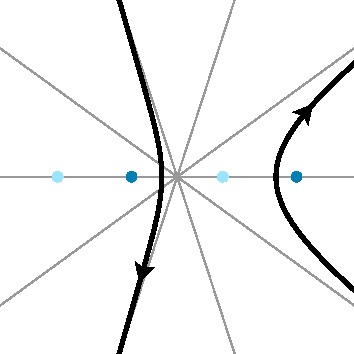
\includegraphics[scale=0.7]{figures/u_contour_5.pdf}
    \hspace{1cm}
    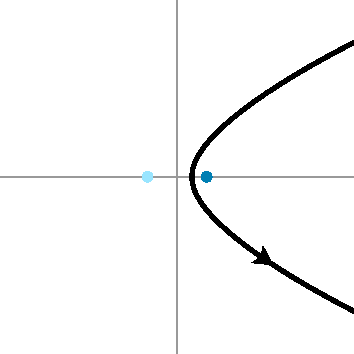
\includegraphics[scale=0.7]{figures/zeta_contour_5.pdf}
    \caption{\textcolor{orange}{Change the pictures with the one centered at the critical values/points respectively}The preimage of a ray departing from the critical value and going to infinity along the positive real axis.}
    \label{fig:thimble_vs_rays}
\end{figure}
Choose $a$ a ciritcal point of $f$ and $\alpha=f(a)$, let $I$ be the thimble integral through the thimble $\Lambda_a^\theta$,
\begin{equation}
I(z)\defeq\int_{\Lambda_a^\theta}e^{-zf}\nu
\end{equation}
our main results show that $I$ is Borel regular as a conseuqence of the fact that thimble integrals can be turned into Laplace transforms. We recall the well-known result
\begin{lemma}[see Lemma \ref{lem:thimble_proj_formula-proof}]\label{lem:thimble_proj_formula}
A function $\iota$ with $I = \laplace_{\zeta, \alpha}^\theta \iota$ is given by the {\em thimble projection formula}
\begin{equation}\label{eqn:formula}
\iota = \frac{\partial}{\partial \zeta} \left( \int_{\Lambda^\theta(\zeta)}\nu \right),
\end{equation}
where $\Lambda^\theta(\zeta)$ is the part of $\Lambda_a^\theta$ that goes through $f^{-1}([\alpha,\zeta e^{i\theta}])$. Notice that $\Lambda(\zeta)$ starts and ends in $f^{-1}(\zeta)$. \textcolor{magenta}{[The thimble $\Lambda$ needs an orientation, but the orientation is arbitrary.]}
\end{lemma}
%\begin{remark}
%The operator $\fracderiv{1/2}{\zeta}{\alpha}$ is the fractional derivative based at $\zeta = \alpha$, as defined in Section~\ref{L-int-op}:
%\begin{align*}
%\partial^{1/2}_{\zeta, \alpha} & \defeq \tfrac{\partial}{\partial \zeta} \, \partial^{3/2}_{\zeta, %\alpha} \\[2mm]
%[\partial^{3/2}_{\zeta, \alpha} g](p) & \defeq \frac{1}{\Gamma(\tfrac{1}{2})} \int_{\zeta = \alpha}^p \big(\zeta(p)-\zeta\big)^{-1/2} g\,d\zeta.
%\end{align*}
%\begin{verify}
%\begin{align*}
%[\partial^{0+1/2}_{\zeta, \alpha} f](p) & = \left(\tfrac{\partial}{\partial \zeta}\right)^{0+1} \partial^{1/2-1}_{\zeta, \alpha} \\
%& = \left(\tfrac{\partial}{\partial \zeta(p)}\right)^{0+1} \frac{1}{\Gamma(1-1/2)} \int_{\zeta = \alpha}^p \big(\zeta(p)-\zeta\big)^{-1/2} f\,d\zeta
%\end{align*}
%\end{verify}
%\end{remark}
Then, Borel regularity for thimble integrals is stated in the following theorem: 
\begin{theorem}[see Theorem \ref{thm:maxim-proof}]\label{thm:maxim}
If the integral defining $I$ is absolutely convergent, then $I$ is Borel regular. More explicitly: 
\begin{enumerate}
\item\label{part-1} As $z \to \infty$ along the ray $z \in e^{-i\theta}\,\R_{>0}$, the function $I$ is asymptotic to a trans-monomial $\tilde{I}\in e^{-z \alpha} z^{-1/2} \C\llbracket z^{-1}\rrbracket$. Recall that $\theta$ is the direction of the ray $\Gamma^\theta_\alpha$.
\item\label{part-2} The series $\tilde{I}$ is $1$-Gevrey. In other words, $\tilde{\iota} \defeq \borel_\zeta \tilde{I}$ converges near $\zeta=\alpha$.
\item\label{part-3} If you continue the sum of $\tilde{\iota}$ along the ray $\Gamma_\alpha^\theta$, and take its Laplace transform along that ray, you'll recover $I$.
\end{enumerate}
\end{theorem}
\color{Goldenrod}
Then, our main result for thimble integrals is proving they are indeed Borel regular:
\begin{theorem}[see Theorem \ref{thm:maxim-dim}]
    Let $\tilde{I}_{j}(z)\in e^{-z \alpha_j} z^{-1/2} \C\llbracket z^{-1}\rrbracket$ be the asymptotic expansion of $I_j$ as $\Re z e^{i\theta}\to \infty$ for the generic direction $\theta$. Then:
\begin{enumerate}
\item The series $\tilde{\Phi}_j:=z^{1/2} \tilde{I}_j$ is $1$-Gevrey, thus $\tilde{\phi}_j(\zeta)\defeq\borel_\zeta(\tilde{\Phi}_j)$ converges near $\zeta=\alpha_j$
\item If you continue the sum of $\tilde{\phi}_j$ along the ray $ e^{i\theta}[\alpha_j,+\infty)$, and take its Laplace transform along that ray, you'll recover $z^{1/2} I_j$.
\item\label{part3} For any $\zeta$ on the ray going rightward from $\alpha_j$, we have a \textit{thimble projection formula}
\begin{multline}
\hat{\phi}_{j}(\zeta)=\fracderiv{3/2}{\zeta}{\alpha_j} \left( \int_{\Lambda_j(\zeta)}\nu \right)=\left(\tfrac{\partial}{\partial \zeta}\right)^2\,\frac{1}{\Gamma\big(\tfrac{1}{2}\big)} \int_{\alpha_j}^\zeta (\zeta-\zeta')^{-1/2}\left( \int_{\Lambda_j(\zeta')} \nu \right)\,d\zeta',
\end{multline}
where $\Lambda_j(\zeta)$ is the part of $\Lambda_j$ that goes through $f^{-1}([\alpha_j, \zeta])$. Notice that $\Lambda_j(\zeta)$ starts and ends in $f^{-1}(\zeta)$. \textcolor{magenta}{[The thimble $\Lambda_j$ needs an orientation, but the orientation is arbitrary.]}
\end{enumerate}
\end{theorem}
\color{black}
We sketch the proofs of the main results in the following diagram (for the rigorous ones see Section~\ref{borel-reg-thimble}):
\[
\begin{tikzcd}
{I} \arrow[rrr,"\aexp^{\theta}"]\arrow[dd, swap,"\laplace^{-1} "] &  & & \tilde{I}\arrow[dd,"\borel"]\\
& & &\\
\iota \arrow[r,equal] & \hat{\iota} & &\tilde{\iota} \arrow[ll, "\text{sum}"]
\end{tikzcd}
\]
On the one hand, with a change of coordinates, the thimble integral $I$ can be written as a Laplace type integral, i.e. as the Laplace transform of a function $\iota$, written explicitly in equation~\eqref{eqn:formula}. 
On the other hand, we compute the asymptotic expansion of $I$ using the saddle point approximation, which turns out to be a formal $1$-Gevrey series in the frequency domain. Consequently, its Borel transform $\series{\iota}$ is a germ of holomorphic functions at $\zeta=\alpha$ in the position domain. Finally, we'll show that the Taylor expansion of $\iota$ at $\zeta=\alpha$ agrees with~$\tilde{\iota}$. 


%% the following remark has been moved to Section of the proof
%\begin{remark}\label{rmk:Pham formula}
%    Equation \eqref{eqn:formula} gives an explicit expression for $\phi_j$ in terms of $\nu$ and of the pre-image of the ray $e^{i\theta}[\alpha_j,\zeta)$ via $f$. When $f$ and $\nu$ are polynomials and $X$ is $N$-dimensional, a result of Pham \cite[Equation 2.4, II partie]{pham} allows to write $\hat{\iota}_j$ explicitly as 
%    \begin{equation}\label{eqn:Pham}
 %       (-1)^{\frac{N(N-1)}{2}}  \sum_{k=0}^\infty c_k\, \delta^{-\frac{N}{2}-k}+ \text{ hol. funct.}
 %   \end{equation}
%for some coefficients $c_k$ which depends on $f$ and $\nu$, and with $\delta^{-\alpha}$ be defined as
 %  \begin{equation*}
  %     \delta^{-\alpha}:=\begin{cases}
   %        \frac{\zeta^{\alpha-1}}{-2\pi i(\alpha-1)!}\log(\zeta) + \text{ hol. funct.} & \text{ if } \alpha\in\mathbb{N}^*\\
    %       & \\
     %      \frac{(-\zeta)^{\alpha-1}}{2\pi i \Gamma(-\alpha)}+ \text{ hol. funct.} & \text{ if } \alpha\notin \mathbb{N}^* 
      % \end{cases}
   %\end{equation*}
%In particular, if $N=1$, from equation \eqref{eqn:Pham} we deduce that $\hat{\phi}_j$ is the $1/2-$ derivative of $\hat{\iota}_j$, \textcolor{orange}{hence it has simple singularities \ref{simple-res-thimble}.} We expect this result to hold beyond the polynomial case. We also expect that equation \eqref{eqn:formula} can be generalized to the $N$-dimensional case replacing the $3/2$-derivative with the $(N+1)/2$ one. 
%\end{remark}
%     
\subsubsection{Other results}
%
As part of the treatment, we have made use of some new perspectives on the Laplace transform (see Section~\ref{sec:Laplace-Borel-general}). Indeed, the Laplace transform is often used to solve ODEs on the frequency domain by relating them to ODEs on the position domain. We find, however, that it is much easier and more natural to relate ODEs on the frequency domain to integral equations on the spatial domain. In particular, working with integral equations in the spatial domain will be our main strategy to prove Borel regularity for ODEs (see \cite[Theorem 4]{reg-sing-volterra}). 

Furthermore, we introduce a geometric picture where the position domain $B$ is a translation surface. If $b \in B$ is non-singular, the frequency domain for $\laplace_b^\theta$ is $T^* B_b$. If $b$ is a conical singularity, the frequency domain is more interesting, as we'll see in our main example (see Figure \ref{fig:different_fibres}). 

\begin{figure}[ht]
\centering
    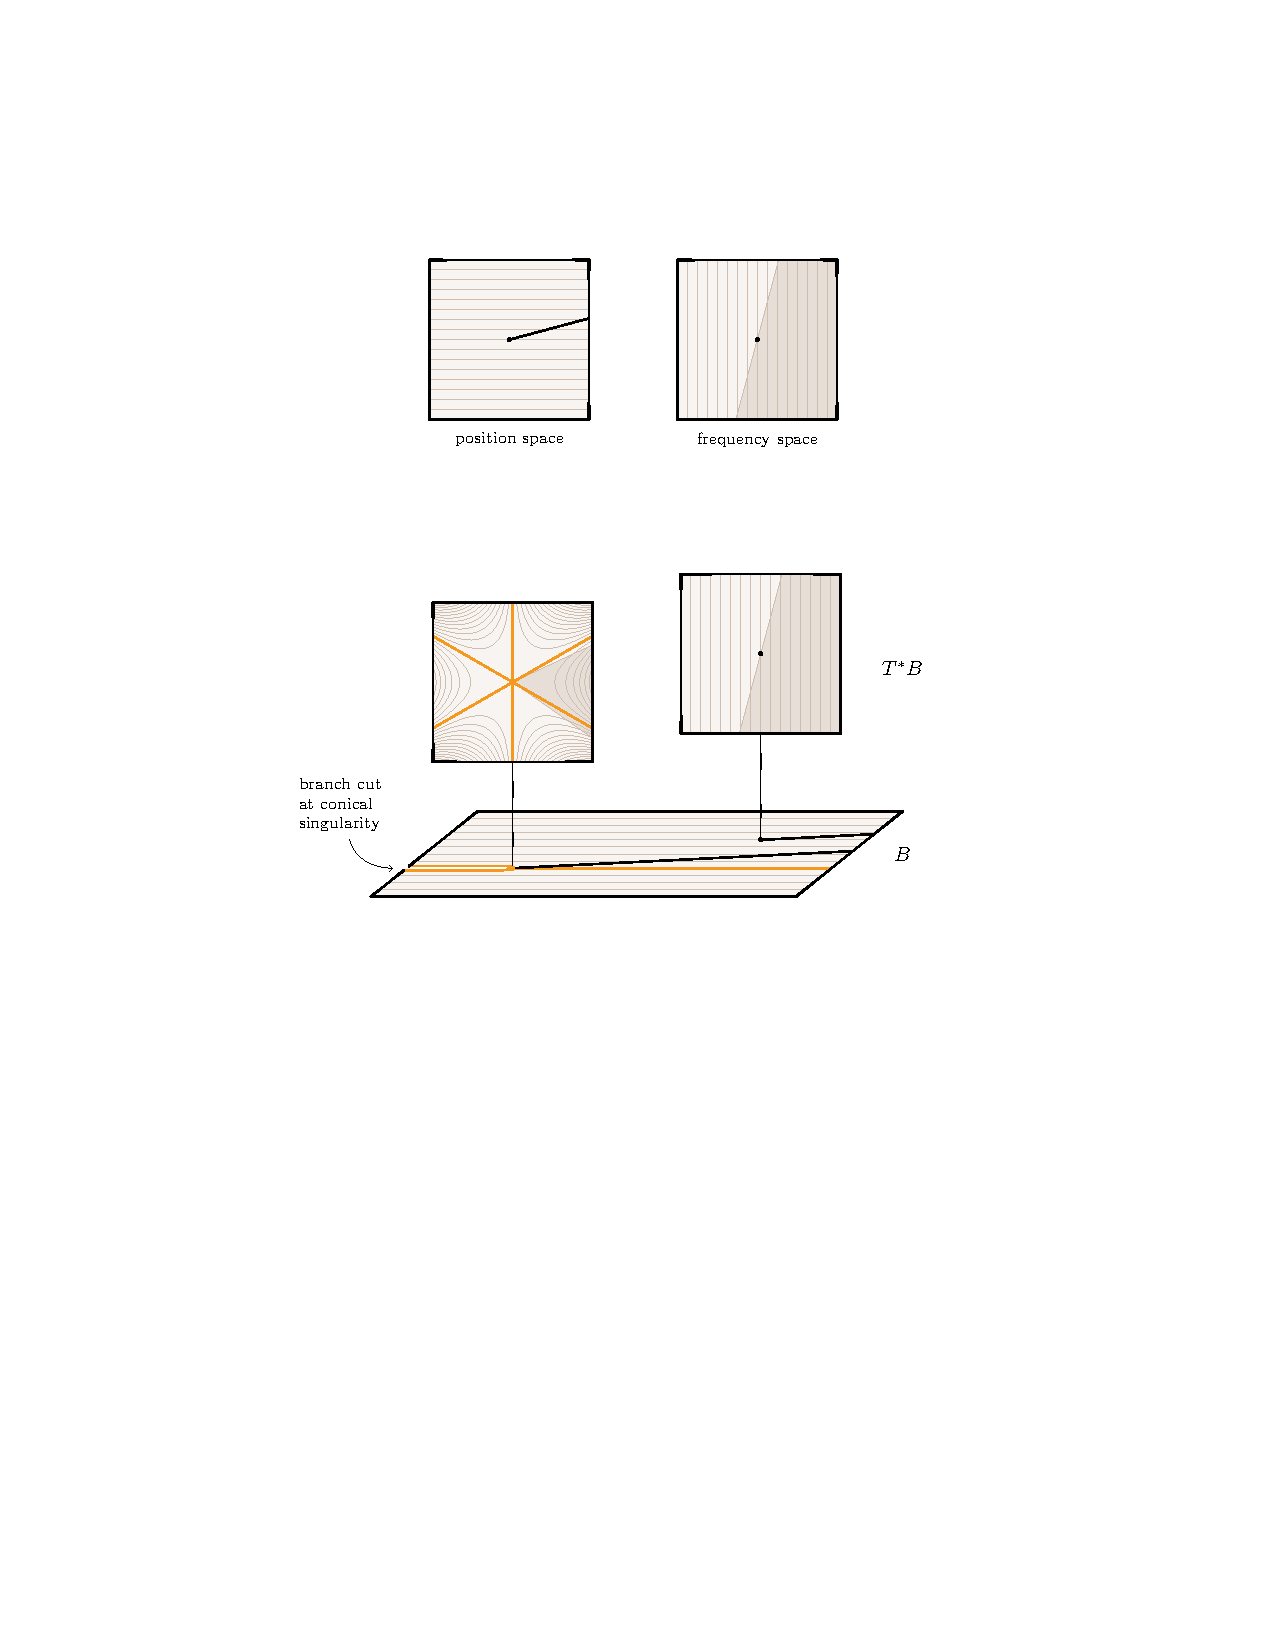
\includegraphics{testbed/testbed1.pdf}
    \caption{The fiber over an ordinary point of the translation surface $B$ is a copy of the complex plane. However, the fiber over a singular point of $B$ has an interesting structure. Here we represent the example of Airy functions, where the singularity as angle $6 \pi$.}
    \label{fig:different_fibres}
\end{figure}
We’ll illustrate our main results with detailed treatments of several examples: we’ll mostly focus on degree two ODEs that admit a frame of solutions expressed as thimble integrals: the Airy--Lucas functions (Section~\ref{example_AL}), modified Bessel function, Airy function (Appendix~\ref{airy-appendix}), \textcolor{red}{the anharmonic oscillator...).} 

On the one hand, we explicitly solve the integral equation associated with the ODE, building a frame of analytic solutions which are Laplace transforms. On the other hand, our \textit{thimble projection reasoning} shows how to rewrite explicitly thimble integrals as a Laplace transform and it makes Borel regularity evident directly from explicit computations. The thimble projection reasoning is the one we use in the proof of Theorem~\ref{thm:maxim} part~\ref{part3}. In the Airy example (see Section~\ref{airy-appendix}) we’ll compute the \textit{thimble projection formula} directly, and by numerical check we show $\hat{\phi}\defeq\fracderiv{-1/2}{\zeta}{\alpha}\iota$ is a simple resurgent function (see Section~\ref{apx:eye-res-airy}).

Among the examples we study, some of them have been discussed many times, using different approaches and conventions. We try to give an idea of how all these different treatments fit together. For instance, for the Airy function we’ll make a comparison with \cite[Section 2.2]{lectures-Marino}, \cite[Section 6.14]{diverg-resurg-i}, and \cite[Section 2.2]{kawai-takei}). \textcolor{red}{The anharmonic oscillator was also discussed in (\cite{bender-wu}, \cite[Appendix B]{aniceto2019primer} and \cite[Section 2.5.3]{sternin1995borel}).} Other examples haven't been discussed much, as for Airy--Lucas functions \cite[Equation 3.2]{charbonnier22}. 

Recently, resurgence theory (first developed by \'Ecalle in the '80) has attracted interest in mathematics and physics. The resurgence of linear ODEs have been intensively studied (see Costin slides for ReNewQuantum, \cite{EcalleIII,loday1994stokes,diverg-resurg--ii}) and many results are also known for non-linear ODEs (see \cite{schiappa-PI,costin-PI,diverg-resurg-iii} \textcolor{magenta}{[check also paper by \'Ecalle and Sauzin]}). For algebraic thimble integrals of the type we studied in this paper, the resurgence of their asymptotic expansion can be understood geometrically (see \cite{Maxim_slide_ERC}, \cite[Section 6.2]{kontsevich2022analyticity}), however for more general exponential integrals (see examples in \cite{Maxim_slide_ERC}) resurgence remains conjectural. Despite their simplicity, our examples of linear ODEs and of 1-dimensional integrals are toy-models that show some features of resurgent functions. 

%\color{gray}
%\begin{itemize}
%\item The central goal of this paper is to lay out two kinds of problems where we can prove that the Borel sum of a formal power series solution is always an actual solution.
%\begin{itemize}
%\item The first problem is evaluating a certain kind of exponential integral: a one-dimensional {\em thimble integral}.
%\item The second problem is solving a certain kind of ODE.
%\item These two problems are closely linked. By playing with derivatives of an exponential integral, you can often find a linear ODE that the integral satisfies. Conversely, for many classical ODEs, there are useful bases of exponential integral solutions.
%\item \textcolor{magenta}{(Does this touch the Picard-Lefshetz perspective? Betti / de Rham relationship: ODE is a connection, and exponential integrals give flat sections?)}
%\end{itemize}
%
%\item Clearly separate the parts of the theory that deal with holomorphic functions and formal power series.
%\begin{itemize}
%\item we can do that also for thimble integrals (this is part 4 of Thm 5.1 in {\tt draft2.pdf})
%\end{itemize}
%\item (Super-motivation: why do the zeroes of $\lambda$ play a special role?) As part of the treatment, we've made use of some new perspectives on the Laplace transform.
%\begin{itemize}
%\item \textbf{Geometric picture.} The spatial domain $B$ is a translation surface. If $b \in B$ is non-singular, the frequency domain for $\laplace_b^\theta$ is $T^* B_b$. If $b$ is a conical singularity, the frequency domain is more interesting, as we'll see in our main example.
%\item \textbf{A new dictionary for ODEs.} The Laplace transform is often used to solve ODEs on the frequency domain by relating them to ODEs on the spatial domain. We find, however, that it's much easier and more natural to relate ODEs on the frequency domain to integral equations on the spatial domain. 
%\begin{itemize}
%\item This clarifies why we take the Borel sums at zeroes of $\lambda$ when we're trying to solve an ODE.
%\end{itemize}
%\end{itemize}
%\item Our picture helps explain why it's useful to work on the Borel plane (the position domain).
%\begin{itemize}
%\item Integral equations are more regular than differential equations.
%\item A thimble integral in the frequency domain can be recast as the Laplace transform of a function in the position domain.
%\end{itemize}
%\item Illustrate with detailed treatments of several examples.
%\begin{itemize}
%\item Contour argument (thimble integrals)
%\item solving integral equation (ODE)
%\item How thimble integrals and ODE are related in our examples?
%\end{itemize}
%\begin{itemize}
%\item Some have been discussed many times, using different approaches and conventions. We'll try to give an idea of how all these different treatments fit together. $\bullet$ The Airy function (Marino, Sauzin). $\bullet$ The anharmonic oscillator (Bender--Wu, Schiappa).
%\item Others haven't been discussed much.
%\end{itemize}
%\item Recently, resurgence theory (first developed by \'Ecalle in the '80) has attracted interests in math and physics as a powerful alternative to Borel summability. Resurgence of lienar ODEs have been studied (see Costin slides for ReNewQuantum). Many results are also known for non linear ODEs (see Schiappa PI, Costin PI). For algebraic exponential integrals of the type we studied in this paper, resurgence of their asymptotic expansion can be understood geometrically (see Maxim's slides ReNewQuantum), however for more general exponential integrals (see examples in Maxim's talk) resurgence remains a conjecture. Despite their simplicity, our examples of linear ODEs and of exponential integrals show some features of resurgence and they are toy model to get a feeling on \'Ecalle formalism.       
%\item \textcolor{magenta}{The examples give a place to compare more complicated formalisms like the Picard-Lefshetz (Morse theory) or Ecalle formalisms? [How do we work this into the introduction?]}
%\begin{itemize}
%\item thimble integrals are geometric in the sense of being pairing between homology and cohomology 
%\item computation of Stokes constants via Picard--Lefschetz theory
%\end{itemize}
%\end{itemize}

%\subsection{Why does Borel resummation work?}
%
%\color{gray}
%
%Borel resummation is a way of turning a formal power series
%\[ \series{\varphi} = z^\sigma \left( \frac{\varphi_0}{z} + \frac{\varphi_1}{z^2} + \frac{\varphi_2}{z^3} + \frac{\varphi_3}{z^4} + \ldots \right), \]
%with $\sigma \in [0, 1)$, into a function which is asymptotic to $\series{\varphi}$ as $z \to \infty$. Different functions can be asymptotic to the same power series, and Borel resummation picks one of them, performing an implicit regularization~\textbf{[arXiv:1705.03071, or maybe arXiv:1412.6614]}. When a function matches the Borel sum of its asymptotic series, we'll say it's {\em Borel regular}. Several familiar kinds of regularity imply Borel regularity, and shed light on why it occurs.
%%%Knowing that a function is Borel regular gives us extra information about it---enough to reconstruct it from its asymptotic series. What's the nature of this extra information?
%%%Since different functions can be asymptotic to the same power series, Borel resummation must involve an {\em implicit regularization}, restricting its range to a class of functions which are uniquely determined by their formal power series.
%\begin{itemize}
%\item \textbf{Having a good asymptotic approximation}
%
%Let $R_N$ be the difference between a function and the partial sum
%\[ \frac{\varphi_0}{z} + \frac{\varphi_1}{z^2} + \frac{\varphi_2}{z^3} + \ldots + \frac{\varphi_{N-2}}{z^{N-1}} \]
%of its asymptotic series. Watson showed a century ago that the function is Borel regular whenever there's a constant $c \in (0, \infty)$ with
%\[ |R_N| \le \frac{c^{N+1} N!}{|z|^N} \]
%over all orders $N$ and all $z$ in a wide enough wedge around infinity (Sokal, ``An improvement of Watson's theorem on Borel summability''; Hardy, {\em Divergent Series}, Theorem~136; Watson, ``A theory of asymptotic series,'' \S 8?).
%\color{black}
%
%\item \textbf{Satisfying a singular differential equation}
%
%\begin{itemize}
%\item This is the setup. We restrict to ODEs with irregular singularity at $\infty$ and of Poincaré rank $1$: 
%\begin{equation}\label{eqn:standard ODE}
%\Big[ P(\partial_z)+\frac{1}{z}Q_1(\partial_z)+\sum_{j=2}^d z^{-j}R_j(\partial_z)\Big]\Psi=0
%\end{equation}
%where $P(\lambda)$ is a (monic) degree $d$ polynomial, $Q(\lambda)$ is a degree $d-1$ polynomial and $R_j$ is a degree $d-j$ polynomial. \textcolor{magenta}{[Looking at the existence theorem in {\tt airy-resurgence} 2.1.3, we could apply this reasoning on the analytic side for more general equations, but this particular case makes it easier to talk about the formal side as well.]} Furthermore we assume $P$ has simple zeros $P(\alpha_j)=0$, $j=1,...,d$ and $Q(\alpha_j)\neq 0$.
%\item \color{DarkTurquoise}
%I think we can go more general? If I'm not mistaken, \'{E}calle's equation form \cite[Equation~2.2.3, p.~105]{EcalleIII} covers operators like
%\[ P(\partial_z) + \frac{1}{z} Q_1(\partial_z) + \frac{1}{z^2}\big[ R_0(z^{-1}) + R_1(z^{-1})\,\partial_z + \ldots + R_d(z^{-1})\,\partial_z^d \b], \]
%where $P$ and $Q$ are as above, and $R_0, \ldots, R_d$ are holomorphic functions on $\C$.
%\color{black}
%\item (backgrounds) Under these assumptions, 
%\begin{itemize}
%\item \eqref{eqn:standard ODE} admits a basis of formal solutions: let $\tau_j:=Q(-\alpha_j)/P'(-\alpha_j)\in\mathbb{Q}^*$, then the formal solutions $\tilde{\Psi}_1,...,\tilde{\Psi}_d$ are of the form \cite{int-irreg} \cite[Proposition~2.2.7, p.~111]{EcalleIII}
%\begin{equation}
%\label{formal solution}
%\tilde{\Psi}_j(z)=e^{-\alpha_j z}z^{-\tau_j}\tilde{F}_j(z)\in e^{-\alpha_j z } z^{-\tau_j}\,\C \llbracket z^{-\tau_j} \rrbracket
%\end{equation}
%Notice that this basis is distinguished only up to scaling, so we have a distinguished frame in the space of formal solutions. 
%\item \eqref{formal solution} is Borel-Laplace summable and its Borel-Laplace sum $\Psi_j$ satisfies the original equation \eqref{eqn:standard ODE}
%\item as a consequence, the distinguished frame of formal solutions become a distinguished frame of analytic solutions $\Psi_1,...,\Psi_d$.  
%\end{itemize}
%\item Can we see there exists a distinguished basis in a purely analytic way? YES. [Thm 1]% The reason is the existence theorem gives for every $\alpha_j$ a unique solution in the $\zeta$-plane which blows-up in a certain way at $\alpha_j$: ${\phi}_j(\zeta_j)=\zeta_j^{-\tau_j}+\tilde{f}_j$, $\zeta_j=\zeta-\alpha_j$.
%\item why Borel summations of $\tilde{\Psi_1},...,\tilde{\Psi_d}$ finds this solutions? because they are an analytic frame of Borel regular functions. 
%\begin{itemize}
%\item {[Thm 1]}: for every $\alpha_j$ there exists a unique solution in the $\zeta$-plane which blows-up in a certain way at $\alpha_j$: ${\phi}_j(\zeta_j)=\zeta_j^{-\tau_j}+\tilde{f}_j$, $\zeta_j=\zeta-\alpha_j$. (proof based on existence theorem \ref{frac_int_exist})
%\item {[Thm 2]}: The Borel sum of the formal solutions $\tilde{\Psi}_j$ are the same as the Laplace transform of the solutions of Thm 1. 
%\item Cor of Thm 2: the Laplace transform of solutions of Thm 1 are Borel regular.   
%\end{itemize}
%\item Say there's a unique solution (up to scaling) that shrinks as you go right; everything else blows up exponentially. Then this is the only solution that can be expressed as a Laplace transform. [Follows from Aaron's argument in Airy resurgence, even if Aaron works with more general ODEs]
%
%\item Draw diagram showing formal vs. holomorphic solutions in time vs. frequency domains.
%
%\begin{center}
%\begin{tikzcd}
%& & ODE\arrow[dd,"\borel"]\arrow[dd,"\laplace^{-1}",swap] & & \\
%\Phi\arrow[rru,dotted, no head, tail] &\textcolor{red}{\hat{\Phi}}\arrow[ur,red, no head, tail] & & & \tilde{\Phi}\arrow[llu,"formal",swap, no head, tail]\arrow[dd,"\borel"]\\
%& & IE & & \\
%\phi\arrow[rru, no head, tail]\arrow[uu,"\laplace"]& \textcolor{red}{\hat{\phi}}\arrow[ur, no head, tail]\arrow[rrr,"sum",mapsfrom,red]\arrow[uu,"\laplace"]& & & \tilde{\phi}\arrow[llu, no head, tail]
%\end{tikzcd}
%\end{center}
%
%where the arrow in red are a consequence of multisummability. In addition, we can distinguish on the right hand side of the diagram the formal solutions and on the left hand side the holomorphic ones. On the upper part of the diagram the functions in the $z$-plane while on the lower part the functions in the Borel plane $\zeta$-plane.
%\item  
%there are many ways to see this problem have a distinguished base of solutions, Poincar\'e see it formally in the $z$-plane, \textcolor{red}{\'Ecalle figured it out how to see it formally in the Borel plane}, our results shows how to see it analytically in  the Borel plane.
%\item  M.A.E.T. says you can start in formal $z$-plane but it is not really constructive (see Balser chap 14); going from formal $\zeta$ to analytic is constructive and it's essentially Borel-Laplace summation. Our method uses just Laplace transform. 
%\item How do we know we are picking the same frame? from properties of Laplace transform we get solution asymptotics to Poincar\'e frame. From uniqueness result we get a frame equivalent to \'Ecalle's frame. 
%\item multi-summability is a regularity result starting form the formal solution in the $z$-plane. Borel regularity is instead based on the analytic solution in the $z$-plane. The argument we gave about getting the same frame is what proves Borel regularity of $\Psi_j$.   
%\end{itemize}
%
%\color{DarkBlue}
%
%\item \textbf{Being a thimble integral}
%
%\begin{itemize}
%\item This is the setup. Let $X$ be an algebraic variety of dimension $N$, $f\colon X\to \mathbb{C}$ be a holomorphic Morse function with only simple critical points and $\nu\in\Gamma(X,\Omega^N)$.
%\begin{itemize}
%\item recall theory of homology and cohomology to define the thimbles integrals. Pham has briefly discussed it, but apparently was introduced by Malgrange, Milnor and ?.  
%\end{itemize} 
%\item background: Pham prove Borel regularity for exponential integral in N-dimension and without assuming Morse critical points (but only isolated). His proof is geometric [it may be useful to add it in Appendix]. 
%\item \textcolor{red}{We give an analytic proof analogous of Pham.}
%\item I think we should separate what can we do in general for N-dimensional integral and what is special for the $1$-dimensional one. 
%\item {[Thm 4]} 1-dim thimbles integrals are Borel regular, namely let 
%\begin{equation}
%I_{\alpha}(z)\defeq\int_{\Lambda_\alpha}e^{-zf}\nu
%\end{equation}
%
%then the following diagram is commutative
%\begin{equation}
%\begin{tikzcd}
%I_{\alpha}(z) \arrow[r,"\ae^\theta"] & \tilde{I}_{\alpha}(z)\arrow[dd,"\borel"]\\
%& \\
%\hat{\iota}_\alpha(\zeta)\arrow[uu, "\laplace^\theta_\alpha "] & \tilde{\iota}_{\alpha}(\zeta) \arrow[l, "\text{sum}"]
%\end{tikzcd}
%\end{equation}
%\begin{itemize}
%\item on the one hand take asymptotic expansion of integral via saddle point approximation and then study the Borel Laplace sum of the divergent series [from left upper corners clockwise]
%\item on the other hand \textcolor{red}{see that the thimble integral is a generalized Laplace transform (which in certain cases can be rewritten as a usual Laplace transform).}
%\item A priori, the Laplace transform of $\hat{\iota}_\alpha(\zeta)$ and $I_{\alpha}(z)$ have the same asymptotic behaviour in a given sector (indeed taking the asymptotic of $I_\alpha(z)$ we \textit{loose} information); however Borel regularity guarantees that $I_{\alpha}(z)=\laplace^{\theta}\hat{\iota}_{\alpha}$ in a given sector.
%\item A corollary of [Thm 4] is the fractional derivative formula.
%\item Conjecturally, we expect $\hat{\varphi}_\alpha(\zeta)$ to have simple singularities. 
%\end{itemize}
%\item From the result of Pham we can deduce Stokes constants are always integers as they are intersection numbers (use same argument of Maxim). See also the argument of KS21 sec 6.2 in the framework of analytic WCFs. Prove integrality of Stokes constants using the fractional integral formula vs differential equation (see example in Appendix C) 
%\end{itemize}



%\subsection{Stokes phenomenon}
%\begin{itemize}
%\item For Bessel functions, we can see explicitly how solutions jump when the Laplace transform angle crosses a critical value.
%\item The jump comes from the branch cut difference identity for hypergeometric functions.
%\item Possible interpretation of the Stokes factors as intersections numbers in Morse--Novikov theory \textbf{[ask Maxim]}
%\end{itemize}
\subsection{Plan of the paper}
The paper is organized as follows: Section~\ref{sec:Laplace-Borel-general} is devoted to define the new geometric picture of the Borel and Laplace transform. The reader who is not familiar with the formalism of Borel and Laplace transforms might start with Sections \ref{sec:reg-decay}, the beginning of Section~\ref{sec:geometry_borel} and of Section~\ref{sec:borel-laplace-homom}. Then, Section~\ref{sec:proof_main_results} contains proofs of the main results: Theorem~\ref{thm2} and Theorem~\ref{thm:maxim}. Finally, in Section~\ref{sec:examples} we give a detailed treatment of different examples both from the ODE perspective and from the thimble integral one. 
We include two appendices: the first one (Appendix~\ref{airy-appendix}) contains a detailed treatment of the Airy example, and it is recommended for readers less familiar to the subject. The second one, Appendix~\ref{apx:generalities_ODEs}, reviews the main aspects of \cite{reg-sing-volterra}.  
%
\subsection{Acknowledgements}
This paper is a result of the ERC-SyG project, Recursive and Exact New Quantum Theory (ReNewQuantum) which received funding from the European Research Council (ERC) under the European Union's Horizon 2020 research and innovation programme under grant agreement No 810573. 

We thank Fondation Mathematique Jacques Hadamard for supporting the visit of the second author at IH\'ES, under the program \textit{Junior Scientific Visibility}. 

We thank Maxim Kontsevich, David Sauzin, Fr\'ed\'eric Fauvet, Andrew Neitzke, for fruitful discussions and suggestions. 
%
\section{Historical context}\label{sec:historical-context}
%
\subsection{Borel regularity as a good approximation condition}
Borel regular functions can be characterized as functions that are approximated well, asymptotically, by polynomials. Watson showed a century ago \cite[Part II, Section 9]{watson2} that a function $F$ is Borel regular whenever its asymptotic expansion for large $|z|$ is uniformly $1$-Gevrey-asymptotic in an obtuse-angled sector at infinity (see Definition~\ref{def:unif-gevrey-asymp}).

Watson's theorem was soon improved by Nevanlinna \cite{nevanlinna} (see a modern proof in \cite[Theorem~B.15]{nikolaev2023exact} and a generalization to power series with fractional power exponents in \cite{delabaere--rosoamanana}), and improved again later by Sokal \cite{sokal1980improvement}. These improvements tell us that the obtuse-angled sector around $\infty$ in the statement above can be replaced with an open disk whose boundary touches infinity---that is, an half-plane which doesn't contain $0$, and may be displaced from $0$ by some distance $c$.
\begin{center}
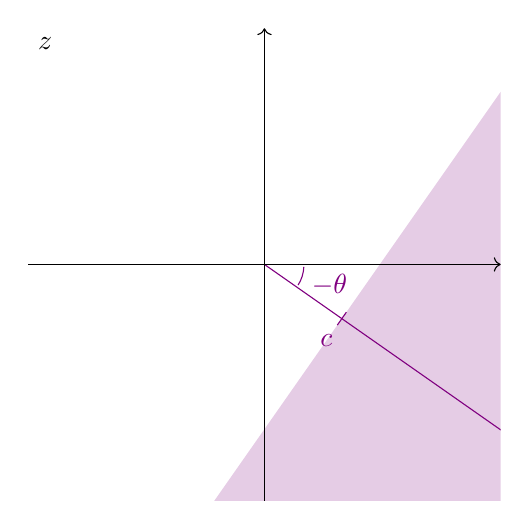
\begin{tikzpicture}
\newcommand{\size}{3}
\pgfmathsetmacro{\outsize}{sqrt(2)*\size}
\newcommand{\ang}{35}
\newcommand{\dis}{1.2}
\begin{scope}
  \clip (-\size, -\size) rectangle (\size, \size);
  \fill[violet!20, rotate=-\ang] (\dis, -\outsize) rectangle (\outsize, \outsize);
  \begin{scope}[violet]
    \draw (0, 0) -- (-\ang:\outsize);
    \draw[rotate=-\ang] (\dis, -0.1) -- (\dis, 0.1);
    \draw[shorten <=0.3mm, shorten >=0.3mm] (0:0.5) arc (0:-\ang:0.5) node[midway, anchor=180-\ang/2] {$-\theta$};
    \node[anchor=90-\ang, inner sep=2mm] at (-\ang:\dis) {$c$};
  \end{scope}
\end{scope}
%%\begin{scope}[violet]
%%  \draw (0, 0) -- (center);
%%  \fill (center) circle (0.05);
%%\end{scope}
\draw[->] (-\size, 0) -- (\size, 0);
\draw[->] (0, -\size) -- (0, \size);
\node[anchor=north west] at (-\size, \size) {$z$};
\end{tikzpicture}
\end{center}
When the half-plane extends along the $-\theta$ direction, the sum $\hat{f}$ of the Borel transform of $\aexp^{-\theta} F$ has an absolutely convergent Laplace transform along the $\theta$ direction. In fact, we have $|\hat{f}| \lesssim e^{c |\zeta|}$ uniformly over all $\zeta$ in a constant-radius neighborhood of the ray $e^{i\theta}[0, \infty)$. 
\begin{center}
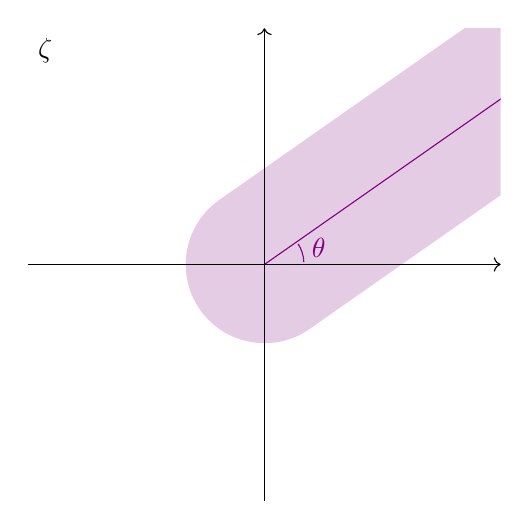
\begin{tikzpicture}
\newcommand{\size}{3}
\pgfmathsetmacro{\outsize}{sqrt(2)*\size}
\newcommand{\ang}{35}
\newcommand{\radius}{1}
\newcommand{\dis}{1.2}
\begin{scope}
  \clip (-\size, -\size) rectangle (\size, \size);
  \fill[violet!20, rotate=\ang] (\outsize, \radius) -- (0, \radius) arc (90:270:\radius) -- (0, -\radius) -- (\outsize, -\radius) -- cycle;
  \begin{scope}[violet]
    \draw (0, 0) -- (\ang:\outsize);
    \draw[shorten <=0.3mm, shorten >=0.3mm] (0:0.5) arc (0:\ang:0.5) node[midway, anchor=180+\ang/2] {$\theta$};
    %%\begin{scope}[rotate=\ang]
    %%  \draw[dotted] (0, 0) -- (0, -\radius) node[anchor=90+\ang] {$r$};
    %%  \draw (\radius, -0.1) -- (\radius, 0.1);
    %%\end{scope}
    %%\fill (mark) circle (0.05);
  \end{scope}
\end{scope}
%%\begin{scope}[violet]
%%  \draw (0, 0) -- (center);
%%  \fill (center) circle (0.05);
%%\end{scope}
\draw[->] (-\size, 0) -- (\size, 0);
\draw[->] (0, -\size) -- (0, \size);
\node[anchor=north west] at (-\size, \size) {$\zeta$};
\end{tikzpicture}
\end{center}

The Watson--Nevanlinna--Sokal characterization of Borel regular functions is totally general, which means it can't take advantage of any extra structure provided by the problem you're trying to solve. We take the opposite approach, showing that certain functions are Borel regular just because of the extra structure provided by the problems they solve. 

%%a function $\Phi$ holomorphic in a sectorial neighbourhood $\mathsf{A}_\theta:=\{z\in\C \vert \Re(e^{i\theta}z)\}$ is Borel regular. Indeed let $\series{\Phi}\in\C\llbracket z^{-1}\rrbracket$ be the ``Gevrey-asymptotics'' of $\Phi$ as $\Re(e^{i\theta}z)\to \infty$, then its Borel transform $\hat{\phi}\defeq\borel\series{\Phi}$ is a germ of holomorphic function at the origin and it can be analytically continued in a tubular neighbourhood of the ray $e^{i\theta}[0,\infty)$ with at most exponential growth at infinity. Hence $\Phi$ is Borel-regularizable. In addition, $\series{\phi}$ converges uniformly to a holomorphic function $\phi(\zeta)$ whose Laplace transform coincides with $\Phi(z)$. In particular, we learn that being ``Gevrey-asymptotic'' to a formal series is a sufficient condition for Borel regularity. 
\subsection{Borel regularity for level~$1$ ODEs}
%
From a formal perspective, the general theory of linear level~$1$ ODEs suggests to look for formal solutions $\tilde{\Psi}_\alpha$ of $\mathcal{P}\Phi=0$ in the transmonomial space $\tilde{\Psi}_\alpha\in e^{-\alpha z} z^{-\tau_\alpha}\C\llbracket z^{-1}\rrbracket$, where $\tau_\alpha=Q(-\alpha)/P’(-\alpha)$~\cite{int-irreg}\cite[Proposition~2.2.7, p.~111]{EcalleIII}. Since the cirtical values are distinct, the transmonomials $\tilde{\Psi}_\alpha$ determine a basis up to scaling, giving the space of formal solutions a distinguished frame. Then, the Main Asymptotic Existence Theorem (M.A.E.T.) guarantees the existence of an analytic frame of solutions asymptotic to the formal one, but it  does not give a way to construct that analytic frame (see~\cite[Chapter 14]{balser}). To get a constructive proof, a classical approach was to investigate Borel summability of the formal solutions~\cite{loday-Remy2011,diverg-resurg--ii,malgrange--fourier,malgrange1995sommation,malgrange92,ramis1991series}. For example, the Ramis Index Theorem shows that the $\tilde{\Psi}_\alpha$ are 1-Gevrey series---the first step in proving Borel~summability~\cite{ramis_index}. \textcolor{orange}{[Mention connection to index, in Loday-Richaud, and to the way orders get shifted?]}

At the same time, a natural question we can ask is whether we can build an analytic frame of solutions, without looking for a formal frame. This is possible, as we proved in~\cite{reg-sing-volterra}, and by our construction, these solutions turn out to be uniform 1-Gevrey asymptotic to the formal solutions $\tilde{\Psi}_\alpha$ (see Corollary~\ref{cor:borel_reg_ODE}). As briefly discussed in Section~\ref{sec:why_borel_ODE} in the sketch the proof of Theorem~\ref{thm:borel_reg_ODE} and Corollary~\ref{cor:borel_reg_ODE}, our result is based on going to the position domain and study solutions of an integral equation with a special behaviour at the singular points $\zeta=\alpha$. Although our approach and the classical one of Borel summability both focus on the importance of the position domain, we study different equations: on the one hand, we solve integral equations in the position domain; on the other hand, Malgrange~\cite{malgrange--fourier} solves differential equations analytically in the position domain, and in~\cite{loday-Remy2011}, Loday-Richaud and Remy solve perturbed integral equations formally in the position domain (following the approach of \'Ecalle~\cite{EcalleIII}). 

\begin{remark}
Our approach of solving regular singular Volterra equation---based on the contraction mapping theorem for suitable Banach spaces \cite{reg-sing-volterra}---is analogous to the one that Braaksma used to solve a different class of non-linear ODEs and difference equations whose coefficients are written as Laplace transforms~\cite{braaksma2006laplace}. What distinguishs our result from the one of Braaksma is to consider the Laplace transform of functions with integrable fractional power singuarities, and even if our result has been proved for linear level~1 ODEs, we allow holomorphic coefficents that are not necesserly Laplace transforms. 

We leave a possible generalization of our result to other classes of ODEs and difference equations for further pubblications. \textcolor{orange}{[Let's do more compare-and-contrast! Our problem space is sort of orthogonal to Braaksma's, but we use the same solution space, so it seems like there could be a cool interaction there.]}
\end{remark}

\begin{remark}
There are many ways to build a frame of solutions for these kinds of ODEs.
\begin{center}
\begin{tabular}{l|l|l}
& \textbf{Analytic} & \textbf{Formal} \\ \hline
\textbf{Frequency domain} &  & Poincar\'{e}: trans-monomial ansatz~\cite{int-irreg} \\ \hline
\textbf{Position domain} & \'{E}calle: resurgence \textcolor{orange}{$\longleftarrow$} & \'{E}calle: formal perturbation theory~\cite{EcalleIII,loday-Remy2011} \\
& Fixed-point iteration~\cite{reg-sing-volterra} \\
\end{tabular}
\end{center}
In the late 1800s, Poincar\'{e} did it formally in the frequency domain~\cite{int-irreg}. In the late 1900s, \'{E}calle and later authors did it formally in the position domain~\cite{EcalleIII,loday-Remy2011}. \'{E}calle also showed that each of his formal solutions sums to a resurgent analytic solution, from which a frame of analytic solutions can be extracted. Most recently, we directly constructed a frame of analytic solutions in the position domain~\cite{reg-sing-volterra}.

In Section~\ref{borel_reg-ODE}, we show that we're all finding the same frame. The uniqueness part of \cite[Theorem~4]{reg-sing-volterra} shows that \'{E}calle's formal solutions sum to our analytic ones, and the properties of the Laplace transform guarantee that our solutions, cast into in the frequency domain, are asymptotic to Poincar\'{e}'s.
\end{remark} 
%
%
%
\subsection{Borel regularity for thimble integrals}
%
Thimble integrals have been studied from different perspectives: in physics, they play an important technical role in quantum mechanics, where infinite-dimensional exponential integrals are supposed to give the expectation values of observable quantities \cite{dunne-unsal2,dunne-unsal,Fauvet_Menous_Queva,Tanizaki:2014tua}. In this context, physicists often use Borel summation, resurgence and related techniques to assign values to these integrals going beyond their pertubative expansion (see also \cite{Berry_Howls,Berry1991,costin_kruskal,Howls97,Howls,pham1988resurgence}). For instance, in complex Chern--Simons theory, one could decompose the path integral in thimble integrals and arguing as in the finite dimesional set-up to study the Witten--Reshetikhin--Turaev invariants of $3$ manifolds \cite{gukov-marino-purtrov-resurgence,Witten}. \textcolor{orange}{Take a look at Witten's paper on knots} More generally, we could think of a problem that is known to admit a thimble integral solution but that's hard to be defined explicitly. However, we know the perturbative expansion of the expected solution; then Borel regularity tells us that the Borel sum of the pertubative series is the solution we're looking for. In fact, the Laplace transform ray (namely the ray along which the Laplace trasnform is defined) is often a ``collapsed'' thimble.\textcolor{Maroon}{This is the bit about turning a perturbative series back into a thimble integral, taking advantage of the fact that the Laplace transform ray is often a ``collapsed'' thimble.}

In the algebraic geometric set-up, namely when $X$ is an $N$-dimensional alegbraic variety over $\C$ and $f$ is a proper map $f\colon X\to\C$, thimble integrals are known as period integrals \cite{deligne2007singularites,Maxim_lectures,pham}.\footnote{In particular, they find application in mirror symmetry for Fano varieties as they encode the Gromov--Witten invariants.\textcolor{orange}{add references---Maxim's mirror symmetry talk, Varchenko}.} In fact, the thimbles represent classes in the homology $H^{B,\theta}_N(X,f)$ which are relative to the preimage of $e^{i\theta}\infty$ under the funtion $f$, for a generic direction $\theta$.\footnote{The relative homology $H_i^{\theta}(X,f)$ is defined as the limit as $c\to e^{i\theta}\infty$, of $H_i^{\theta}(X,f^{-1}(S_c^+))$, where $S_c^+=\lbrace \zeta\in\C \vert \Re \zeta> c\rbrace$. Generic directions correspond to $\theta\neq \arg (\alpha-\beta)$. } Furthermore, if $f$ has non-degenerate critical points, they form a basis for $H_N^{B,\theta}(X,f)$. Then varying $\theta$, $H_N^{B,\theta}(X,f)$ forms a local system over $S^1=\R/2\pi \Z$ singular at $\theta=\arg(\alpha-\beta)$, and whose monodromy can be computed by Picard--Lefschetz formula (we refer to \cite[Section~1]{Arnold} and \cite[Section~3.3, Part II]{pham}). Equivalently, the monodromy data can be computed as the Stokes phenomena for Laplace transforms; indeed as a consequence of our Borel regularity result Theorem~\ref{thm:maxim}, thimble integrals can be turned into Laplace transforms.  

Classical examples of thimble integrals (with polynomial $f$) are special functions, thus the Borel summability properties of their asymptotics can be studied either analytically (through the \textit{thimble projection reasoning} see the discussion in Section~\ref{sec:examples}) or geometrically (in terms of a certain Riemann--Hilbert problem \cite{Maxim_slide_ERC}\cite[Section 6.2]{kontsevich2022analyticity}). 


In the $N$-dimensional analog of our set-up \ref{borel-reg:explanatory-power} the thimbles are actually steepest descent paths from the critical points; thus the asymptotic behaviour as $z\to e^{i\theta}\infty$ can be studied using the steepest descent method \cite{andersen2020resurgence,delabaere-howls,delabaere_dillinger_pham,Delabaere-Pham99,dingle1973asymptotic,Malgrange22,Pham83}.\footnote{In fact, analougus results hold when $f$ satisfies milder assumptions (see for instance~\cite[Section 1.2.2]{mistegard_phdthesis}).} However, the asymptotics of thimble integrals is typically a formal power series, and choosing a suitable resummation technique one should be able to recover the original function. This raises the question we address in this paper, namely to understand why Borel summation is effective for $1$-dimensional thimbles integrals. In a nutshell, our result follows from the fact that thimble integrals are generalized Laplace transforms, hence they are Borel regular functions. In addition, our approach wants to focus on the role of the position domain and it emphasizes how the geometry of the Laplace transform is the natural framework to describe Borel regularity for thimbles integrals (see Fenyes's lecture~\cite{Fenyes-ihes-lecture} and Section~\ref{sec:Laplace-Borel-general}).   

 %In addition, they typically come as \textcolor{orange}{[Stokes phenomena in one case ... in the other is ...]}   


%\textcolor{orange}{hyperasymptotics \cite{Berry_Howls,Berry1991,Howls97,Howls}}
%\color{DarkTurquoise}
%These questions have been classically addressed by Pham \cite[Section 3.3]{pham}, Malgrange \cite[Theorem 6]{Malgrange22}, Berry and Howls \cite{Berry_Howls} and Sternin and Shatalov \cite[Theorem 3.9 and 3.10]{sternin1995borel}. In addition, the study of thimble integrals plays an important technical role in quantum mechanics, where infinite-dimensional exponential integrals are supposed to give the expectation values of observable quantities. Physicists often use Borel summation, resurgence and related techniques to assign values to these integrals \cite{costin_kruskal,pham1988resurgence}.
%\color{black}
%%Our approach wants to focus on the role of the position domain and it emphasizes how the geometry of the Laplace transform is the natural framework to describe Borel regularity for thimbles integrals (see Fenyes's lecture \cite{Fenyes-ihes-lecture}). In a nutshell, we use that thimble integrals are generalized Laplace transforms, to show they are indeed Borel regular functions.  
%     
\section{The Laplace and Borel transforms}\label{sec:Laplace-Borel-general}
\subsection{The geometry of the Laplace transform}
Classically, the Laplace transform turns functions on the position domain into functions on the frequency domain. In the study of Borel summation and resurgence, it's useful to see the position domain as a {\em translation surface} $B$, and the frequency domain as one of its cotangent spaces. Roughly speaking, the Laplace transform lifts holomorphic functions on $B$ to holomorphic functions on $T^*B$.
%
\subsubsection{Translation surfaces, briefly}
%
A translation surface is a Riemann surface $B$ carrying a holomorphic $1$-form $\lambda$~\cite{zorich2006flat}. A translation chart is a local coordinate $\zeta$ with $d\zeta = \lambda$. The standard metric on $\C$ pulls back along translation charts to a flat metric on $B$, with a conical singularity of angle $2\pi n$ wherever $\lambda$ has a zero of order $n-1 > 0$. We'll require $B$ to be finite-type and $\lambda$ to have a pole at each puncture. This kind of translation surface has a ``cylindrical end'' (see Figure \ref{fig:translation_surface}) at each puncture where $\lambda$ has order $-1$, and a ``$|2n|$-planar end'' (see Figure \ref{fig:translation_surface}) at each puncture where $\lambda$ has order $n-1 < -1$~\cite[Section 2.5]{gupta2013meromorphic} \textcolor{orange}{(or cite Aaron's article, which will hopefully present the same background in the translation surface context)}.
\begin{figure}[ht]
    \centering
    %\includegraphics{}
    \caption{On the left an example of translation surface with ``cylindrical end''. On the right, an example of translation surface with  ``$|2n|$-planar end''. }
    \label{fig:translation_surface}
\end{figure}
%
\subsubsection{Direction}\label{transl:dir}
%
The translation structure gives $B$ a notion of direction as well as distance. Away from the zeros of $\lambda$, which we'll call {\em branch points}, we can talk about moving upward, rightward, or at any angle, just as we would on $\C$. At a branch point of cone angle $2\pi n$, we can also talk about moving upward, rightward, or at any angle in $\R/2\pi\Z$, but here there are $n$ directions that fit each description. To make this more concrete, note that around any point $b \in B$, there's a unique holomorphic function $\zeta_b$ that vanishes at $b$ and has $d\zeta_b = \lambda$. \textcolor{VioletRed}{[If we define ``translation parameter'' earlier, we can say:] there's a unique translation parameter $\zeta_b$ that vanishes at $b$.} This function is a translation chart when $b$ is an ordinary point, and an $n$-fold branched covering when $b$ is a branch point of cone angle $2\pi n$. In either case, $\zeta_b \in e^{i\theta} [0, \infty)$ is a ray or a set of rays leaving $b$ at angle $\theta \in \R/2\pi\Z$.
%

Near each branch point $b$, let's fix a coordinate $\omega_b$ with $\zeta_b = \tfrac{1}{n} \omega_b^n$, where $2\pi n$ is the cone angle at $b$. This lets us label each direction at $b$ with an ``extended angle'' in $\R/2\pi n\Z$. Of course, there are $n$ different choices for $\omega_b$.
%
\subsubsection{Frequency}\label{transl-freq}
%
The translation structure also gives us an isomorphism $z \maps T^*_bB \to \C$ when $b \in B$ is an ordinary point, and an isomorphism $z \maps T^*_bB^{\otimes n} \to \C$ when $b$ is a branch point of cone angle $2\pi n$ \textcolor{orange}{[make it clear that $z$ is an almost-global chart on $T^*B$---for example, writing $z\colon T^*B\to\C^2$]}. At an ordinary point, we can define $z$ simply as the map
\begin{align*}
z \maps T^*_bB & \to \C \\
\lambda\big|_b & \mapsto 1.
\end{align*}
To get a definition that generalizes to branch points, though, it's worth taking a fancier point of view. Recall that $T^*_bB = \van_b / \van_b^2$, where $\van_b$ is the ideal of holomorphic functions that vanish at $b$. Observing that $(f + \van_b)^n$ lies within $f^n + \van_b^{n+1}$ for any $f \in \van_b$, we can identify $T^*_bB^{\otimes n}$ with $\van_b^n / \van_b^{n+1}$ for $n \ge 1$. When $b$ is an ordinary point, the function $\zeta_b$ defined in Section~\ref{transl:dir} represents a nonzero element of $\van_b / \van_b^2$: the cotangent vector $\lambda\big|_b$. In general, $\zeta_b$ represents a nonzero element of $\van_b^n / \van_b^{n+1}$, where $2\pi n$ is the cone angle at $b$. We define $z$ as the isomorphism
\begin{align*}
z \maps \van_b^n / \van_b^{n+1} & \to \C \\
\zeta_b + \van^{n+1} & \mapsto 1.
\end{align*}
When $b$ is a branch point, the coordinate $\omega_b$ we chose in Section~\ref{transl:dir} gives us an isomorphism
\begin{align*}
w_b \maps T^*_bB & \to \C \\
\omega_b + \van^2 & \mapsto 1
\end{align*}
that makes the diagram
\begin{center}
\begin{tikzcd}
T^*_bB^{\otimes n} \arrow[r,"z"] & \C \\
T^*_bB \arrow[u,"\blankbox^n"] \arrow[r,"w"'] & \C \arrow[u,"\blankbox^n"']
\end{tikzcd}
\end{center}
commute.
\subsubsection{Boundary}
\textcolor{red}{\textbf{Discuss the visual boundary, citing Lemma~3.1 of Dankwart's thesis \textit{On the large-scale geometry of flat surfaces} for the description of geodesics.}}
%
\subsubsection{The Laplace transform over an ordinary point}\label{laplace:ordinary}
Pick a local holomorphic function $\zeta$ on $B$ with $d\zeta = \lambda$, and an extended angle $\theta \in \R$. \textcolor{VioletRed}{[If we define ``translation parameter'' earlier, we can say:] Pick a translation parameter $\zeta$.} The {\em Laplace transform} $\laplace_\zeta^\theta$ turns a local holomorphic function $f$ on $B$ into a local holomorphic function on $T^*B$. When $b \in B$ is an ordinary point, $\laplace_\zeta^\theta f$ is defined on $T_b^*B$ by the formula
\begin{equation}\label{laplace:int}
\laplace_{\zeta}^\theta f\big|_b = \int_{\Gamma_{b}^\theta} e^{-z\zeta} f\,d\zeta,
\end{equation}
where $z$ is the frequency function and $\Gamma_{b}^\theta$ is the ray that leaves $b$ at angle $\theta$. We’ll use the shorthand $\laplace_{\zeta, b}^\theta f := \laplace_\zeta^\theta f \big|_{\zeta = b}$ throughout this document.

To make sense of this formula, we ask for the following conditions.
\begin{itemize}
\item The base point $b$ is in the domain of $\zeta$. Once we have this, we can continue $\zeta$ along the whole ray $\Gamma_b^\theta$.
\item The ray $\Gamma_b^\theta$ avoids the branch points after leaving $b$.
\item The integral converges. We guarantee this by asking for a pair of simpler conditions.
%\color{RoyalBlue}
\begin{itemize}
\item With respect to the flat metric, $f$ is uniformly of exponential type $\Lambda$ along $\Gamma_b^\theta$, and is locally integrable throughout.\footnote{Recall that a function is of exponential type $\Lambda$ if for every $\varepsilon>0$ there is a constant $A_\varepsilon$ (which depends on $\varepsilon$) such that $|f(x)|\leq A_\varepsilon e^{\Lambda+\varepsilon} $. We instead require that there exists a uniform constant $A$ such that for every $\varepsilon>0$ the bound holds.} Following \cite{reg-sing-volterra}, we require $f\in\singexp{\sigma}{\Lambda}(\Omega_b)$ with $\sigma>-1$.\footnote{The condition $\sigma>-1$ guarantees the integrability at $\zeta=b$.} The set $\Omega_b$ is a tubular neighbourhood of $\Gamma_b^\theta$. 
\item The value of $z$ is in the half-plane $H_{\theta}$ centered around the ray $e^{-i\theta} [0, \infty)$.
\end{itemize}
\end{itemize}
\color{black}
\subsubsection{The Laplace transform over a branch point}
When $b$ is a branch point, we can still use formula~\eqref{laplace:int} to define $\laplace_\zeta^\theta f$ on $T_b^*B$, as long as we take care of a few subtleties. Thanks to the labeling choices we made at the end of Section~\ref{transl:dir}, the extended angle $\theta \in \R$ still picks out a ray $\Gamma_b^\theta$. The function $z$ is defined on $T_b^*B^{\otimes n}$, where $2\pi n$ is cone angle at $b$, so we pull it back to $T^*_bB$ along the $n$th-power map. This amounts to substituting $w_b^n$ for $z$ in formula~\eqref{laplace:int}. The half-plane $z \in H_{\theta}$ in $T_b^*B^{\otimes n}$ pulls back to $n$ sectors of angle $\pi/n$ in $T_b^*B$. We only define $\laplace_\zeta^\theta f$ on one of them: the one centered around the ray $w_b \in e^{-i\theta/n}[0, \infty)$.
%\color{gray}
%\subsection{The geometry of the Borel transform}
%\begin{itemize}
  %\item The Borel transform $\borel\textcolor{orange}{_\zeta}$ turns formal power series in $z^{-1}$---which represent functions defined all non-singular cotangent spaces---into formal power series in $\zeta$. It's a formal inverse of the $\laplace_{\zeta, 0}$.
  %\item Formalizing the change of variable identity that relates $\laplace_{\zeta, \alpha}$ to $\laplace_{\zeta_\alpha, 0}$, we can extend the Borel transform to trans-series, defining $\borel\textcolor{orange}{_\zeta} \maps e^{-\alpha z} \C\llbracket z^{-1} \rrbracket \to \C\llbracket \zeta \rrbracket$ as the formal inverse of $\laplace_{\zeta, \alpha}$.
  %\begin{itemize}
   % \item In other words, when $\borel_\zeta$ acts on formal power series, it formally inverts $\laplace_\zeta$ on the cotangent fiber over $0$. \textcolor{magenta}{When it acts on other trans-monomials, it formally inverts $\laplace_\zeta$ on other cotangent fibers. [Not quite\ldots figure out how to make this precise.] }
  %\end{itemize}
  %\item consequently, $\borel_{\zeta_\alpha}$ acts on trans-monomials $e^{z\alpha}\C\llbracket z^{-1}\rrbracket$ and it formally inverts $\laplace_{\zeta_\alpha}$ on the cotangent fibre over $0$. 
%\end{itemize}
%\color{black}
\subsubsection{Change of translation chart}\label{sec:change-translation}
Let $b \in B$ be an ordinary point, and let $\zeta_b$ be the coordinate on $B$ for which $\zeta = \zeta(b) + \zeta_b$. Then the Laplace transform $\laplace_{\zeta_b,0}$, which turns functions on $B$ into functions on $T^*_{b}B$, is compatible with $\laplace_{\zeta,b}$.  
\begin{lemma}\label{translation}
Let $\varphi\in\singexp{\sigma}{\Lambda}(\Omega_b)$ with $\sigma>-1$ and for some $\Lambda>0$, then
   \begin{equation}
    \label{change-chart}
    e^{-bz} \laplace_{\zeta_b, 0} \varphi = \laplace_{\zeta, b} \varphi.
\end{equation}
In other words, the diagram 
\begin{center}
\begin{tikzcd}
 \mathcal{O}_{T^*B}(H) \arrow[rr, "e^{bz}"]&  & e^{bz}\,\mathcal{O}_{T^*B}(H)\\
& \singexp{\sigma}{\Lambda}(\Omega_b) \arrow[ul, "\laplace_{\zeta_b,0}"]\arrow[ur,swap,"\laplace_{\zeta,b}"]  &  
\end{tikzcd}
\end{center}
commutes, where $H$ is the half-plane $\Re(z) > 0$ (\textcolor{orange}{the coordinate $z$ is a global coordinate on $T^*B$}).
\end{lemma}
\begin{proof}
With a change of variable in the integral that defines the Laplace transform, we see that
\begin{align*}
\laplace_{\zeta, b} \varphi & = \int_{\Gamma_{\zeta,b}} e^{-z \zeta}\,\varphi\;d\zeta \\
& = \int_{\Gamma_{\zeta_b,0}} e^{-z(b + \zeta_b)}\,\varphi\;d\zeta_b \\
& = e^{-b z} \int_{\Gamma_{\zeta_b,0}} e^{-z\zeta_b}\,\varphi\;d\zeta_b \\
& = e^{-b z} \laplace_{\zeta_b, 0} \varphi.
\end{align*}
\end{proof}
We now consider a rescale of the translation structure of $B$, expanding displacements by a factor of $\mu \in (0, \infty)$. The coordinate $\xi = \mu\zeta$ is a chart for the new translation structure. The corresponding frequency coordinate $x \maps T^*B \to B$ is given by $d\xi \mapsto 1$, so $x = \mu^{-1} z$. 
\begin{lemma}
Let $\varphi\in\singexp{\sigma}{\Lambda}(\Omega)$ with $\sigma>-1$ and for some $\Lambda>0$, then
    \[ \laplace_{\xi, 0} \varphi = \mu\,\laplace_{\zeta, 0} \varphi. \]
\end{lemma}
\begin{proof}
    From the computation 
    \begin{align*}
\laplace_{\xi, 0} \varphi & = \int_{\Gamma_{\xi, 0}} e^{-x\xi}\,\varphi\;d\xi \\
& = \int_{\Gamma_{\zeta, 0}} e^{-z \zeta}\,\varphi\;\mu\,d\zeta \\
& = \mu\,\laplace_{\zeta, 0} \varphi
\end{align*}
we get the desired result. 
\end{proof}
%
%Note that $\laplace_{\xi, 0}$ is defined in the new translation structure on $B$, while $\laplace_{\zeta, 0}$ is defined in the old translation structure. We can still compare them because they both turn complex-valued functions on $B$ into holomorphic functions on $T^*B$.
\subsection{Analysis of the Laplace transform}\label{sec:laplace_analytic}

\subsubsection{Regularity and decay properties}\label{sec:reg-decay}
%
Let $\Omega_b \subset B$ be an open, simply connected set that touches but does not contain $\zeta=b$ (see Figure \ref{Fig:domain}). Suppose $\Omega_b$ contains the ray $\Gamma_{\zeta,b}^\theta$. In \cite{reg-sing-volterra} we introduce the function space $\singexp{\sigma}{\Lambda}(\Omega_b)$ of holomorphic functions on $\Omega_b$ which are uniformly of exponential type $\Lambda$ and blow up like $|\zeta|^\sigma$ as $\zeta$ approaches $b$. When $\sigma>-1$, the singularity at $\zeta=b$ is integrable. Hence, the Laplace transform $\laplace_{\zeta, b}^\theta$ turns elements of $\singexp{\sigma}{\Lambda}(\Omega_b)$ into well-defined holomorphic functions on the half-plane $\Re(e^{i\theta} z) > 0$ in the fiber $T_{\zeta=b}^*B$~\cite[Section  5.6]{diverg-resurg-i}.
%Let's say a function $f$ is in $O_{\zeta, \alpha \leftarrow}(g)$ or $O_{\zeta, \alpha \rightarrow}(g)$, respectively, if $|f| \lesssim g$ on some neighborhood of the starting point or infinite end of $\Gamma_{\zeta, \alpha}$. A function is {\em subexponential} along $\Gamma_{\zeta, \alpha}$ if it's in $O_{\zeta, \alpha \rightarrow}(e^{c\zeta})$ for all $c > 0$ \textcolor{magenta}{[shall we write in formula?]}. Let $\mathcal{E}_{\zeta, \alpha}$ be the space of functions that are subexponential on $\Gamma_{\zeta, \alpha}$, integrable at the starting point, and locally integrable throughout. If $f$ is in $\mathcal{E}_{\zeta, \alpha}$, then $\laplace_{\zeta, \alpha} f$ is well-defined and holomorphic for $\Re(z) > 0$ on the part of $T^*B$ that lies over $\Gamma_{\zeta, \alpha}$~\cite[Section  5.6]{diverg-resurg-i}.

\color{RoyalBlue}{$\singexpalg{\sigma}(\Omega_\alpha^\Lambda)$}
\color{Maroon}
Suppose $\Omega_\alpha$ is an open sector with $\zeta = \alpha$ at its tip, and an opening angle of $\pi$ or less. In this case, for any $\Lambda \in \R$, let \textcolor{magenta}{$\widehat{\Omega}_\alpha^\Lambda$} $\dualsector{\alpha}{\Lambda}$ be the union of the half-planes $\Re(e^{i\theta} z) > \Lambda$ over all angles $\theta$ in the opening of $\Omega_\alpha$. Then, let $\dualsingexp{\sigma}{\Lambda}(\Omega_\alpha)$ be the space of holomorphic functions $F$ on $\widehat{\Omega}_\alpha^\Lambda$ with $|F| \lesssim \Delta^\sigma$, where $\Delta$ is the distance to the boundary of $\widehat{\Omega}_\alpha^\Lambda$. The norm $\|F\|_{\sigma, \Lambda} = \sup_{\widehat{\Omega}_\alpha^\Lambda} \Delta^{-\sigma} |F|$ turns $\dualsingexp{\sigma}{\Lambda}(\Omega_\alpha)$ into a Banach space. \textcolor{orange}{Cite \cite{sternin1995borel} better for the theorem.}
\begin{prop}[following~\cite{sternin1995borel}]\label{prop:laplace-cont}
Let $\Omega_\alpha$ be an open sector with $\zeta = \alpha$ at its tip, and an opening angle of $\pi$ or less. For any $\sigma > 0$ and $\Lambda \ge 0$, and any angle $\theta$ in the opening of $\Omega_\alpha$, the Laplace transform $\laplace_{\zeta_\alpha, 0}^\theta$ is a continuous map $\singexp{\sigma-1}{\Lambda}(\Omega_\alpha) \to \dualsingexp{-\sigma}{\Lambda}(\Omega_\alpha)$, with a norm of at most $\Gamma(\sigma)$.
\end{prop}
\begin{proof}
Given some $f \in \singexp{\sigma-1}{\Lambda}(\Omega_\alpha)$, we compute
\begin{align*}
|\laplace_{\zeta_\alpha, 0}^\theta f| & = \left| \int_{\Gamma_{\zeta, \alpha}^\theta} e^{-z\zeta_\alpha} f\,d\zeta_\alpha \right| \\
& \le \int_{\Gamma_{\zeta, \alpha}^\theta} e^{-\Re(z\zeta_\alpha)} |\zeta_\alpha|^{\sigma-1} e^{\Lambda |\zeta_\alpha|} \|f\|_{\sigma-1, \Lambda}\,|d\zeta_\alpha| \\
& \le \int_{\Gamma_{\zeta, \alpha}^\theta} e^{(\Lambda - c_{z, \theta}|z|)|\zeta_\alpha|} |\zeta_\alpha|^{\sigma-1} \|f\|_{\sigma-1, \Lambda}\,|d\zeta_\alpha|,
\end{align*}
where $c_{z, \theta}$ is the cosine of $\arg(z) + \theta$. When $|z|$ is large and $c_{z, \theta}$ is positive, the integrand shrinks exponentially as $|\zeta|$ grows. This shows that for each angle $\theta$ in the opening of $\Omega_\alpha$, the integral defining $\laplace_{\zeta_\alpha, 0}^\theta f$ converges in some region of $\widehat{\Omega}_\alpha^\Lambda$. It also shows that for different angles $\theta$, the functions $\laplace_{\zeta_\alpha, 0}^\theta f$ match where their domains overlap. We can therefore glue these functions together into one big Laplace transform of $f$, defined at large values of $|z|$ across the whole opening angle of $\widehat{\Omega}_\alpha^\Lambda$.

We can now simplify the calculation of $\laplace_{\zeta_\alpha, 0}^\theta f$ by looking at $\arg(z)$ and using the closest angle $\theta$ in the opening of $\Omega_\alpha$. This keeps $\Lambda - c_{z, \theta}|z|$ equal to $\Delta$, the distance to the boundary of $\widehat{\Omega}_\alpha^\Lambda$. It follows that
\begin{align*}
|\laplace_{\zeta_\alpha, 0}^\theta f| & \le \int_{\Gamma_{\zeta, \alpha}^{\arg(z)}} e^{-\Delta|\zeta_\alpha|} |\zeta_\alpha|^{\sigma-1} \|f\|_{\sigma-1, \Lambda}\,|d\zeta_\alpha| \\
& = \int_0^\infty e^{-\Delta t} t^{\sigma-1} \|f\|_{\sigma-1, \Lambda}\,dt.
\end{align*}
The integral on the last line converges throughout $\widehat{\Omega}_\alpha^\Lambda$. We can evaluate it by observing that this bound on the Laplace transform of $f$ is itself a Laplace transform:
\[ |\laplace_{\zeta_\alpha, 0}^\theta f| \le \Gamma(\sigma) \Delta^{-\sigma} \|f\|_{\sigma-1, \Lambda}. \]
In terms of the metric on $\dualsingexp{-\sigma}{\Lambda}(\Omega_\alpha)$ defined above, this bound says that
\[ \|\laplace_{\zeta_\alpha, 0}^\theta f\|_{\sigma, \Lambda} \le \Gamma(\sigma) \|f\|_{\sigma-1, \Lambda}, \]
which is what we wanted to show.
\end{proof}
\begin{prop}
Let $\Omega_\alpha$ be an open sector of the kind described in Proposition~\ref{prop:laplace-cont}, and let $\Omega_\alpha^\varepsilon \subset \Omega_\alpha$ be the open sector created by cutting a sector of angle $\varepsilon > 0$ off each edge of $\Omega_\alpha$. Choose any $\lambda' > \Lambda$. Under the conditions of Proposition~\ref{prop:laplace-cont}, the Laplace transform
\[ \laplace_{\zeta_\alpha, 0}^\theta \maps \singexp{\sigma-1}{\Lambda}(\Omega_\alpha) \to \dualsingexp{-\sigma}{\Lambda}(\Omega_\alpha) \]
has a continuous left inverse
\[ \left(\laplace_{\zeta_\alpha, 0}^\theta\right)^{-1} \maps \dualsingexp{-\sigma}{\Lambda}(\Omega_\alpha) \to \singexp{\sigma-1}{\lambda'}(\Omega_\alpha^\varepsilon), \]
with a norm of at most
\[ \frac{\Gamma(1-\sigma)}{\pi\,\sin(\varepsilon/2)}. \]
\end{prop}
\begin{proof}
Define the sector $\Omega_\alpha^{\varepsilon/2} \subset \Omega_\alpha$ similarly to $\Omega_\alpha^\varepsilon$. Choosing some $\lambda' > \Lambda$, let $\widehat{\Omega}_\alpha^{\varepsilon/2, \lambda'} \subset \widehat{\Omega}_\alpha^\Lambda$ be the union of the half-planes $\Re(e^{i\theta} z) > \lambda'$ over all angles $\theta$ in the opening of $\Omega_\alpha^{\varepsilon/2}$. The boundary of $\widehat{\Omega}_\alpha^{\varepsilon/2, \lambda'}$ forms a path $\textcolor{magenta}{\Lambda}$, which we orient so that the boundary of $\widehat{\Omega}_\alpha^\Lambda$ is on its left. Parameterize $\textcolor{magenta}{\Lambda}$ using the arc length parameter $t$ which is zero at the midpoint of the circular arc part of $\textcolor{magenta}{\Lambda}$. Along $\Lambda$, we have
\[ \Delta \ge \mu + \sin(\varepsilon/2)\,|t|, \]
for some $\mu \in (\lambda, \lambda')$, where $\Delta$ is still the distance to the boundary of $\widehat{\Omega}_\alpha^\Lambda$. On $\Omega_\alpha^\varepsilon \times \textcolor{magenta}{\Lambda}$, we have
\[ \Re(z\zeta_\alpha) \le |\zeta_\alpha| \big(\lambda' - \sin(\varepsilon/2)\,|t|\big). \]

%%Choose a path $\textcolor{magenta}{\Lambda}$ through $\widehat{\Omega}_\alpha^\Lambda$ on which
%%\[ \Delta = m + \sin(\varepsilon)\,|t|, \]
%%where $t$ is an arc length parameter.

%Choose any path $\textcolor{magenta}{\Lambda}$ that runs through $\widehat{\Omega}_\alpha^\Lambda$ at a constant distance from the boundary, oriented so that the boundary is on its left. The inverse Laplace transform is given by the formula

The inverse Laplace transform is given by the formula
\[ \big(\laplace_{\zeta_\alpha, 0}^\theta\big)^{-1} F = \frac{1}{2 \pi i} \int_{\textcolor{magenta}{\Lambda}} e^{z\zeta_\alpha} F\,dz. \]
When $F$ is in $\dualsingexp{-\sigma}{\Lambda}(\Omega_\alpha)$, we have the bound
\begin{align*}
\left|\big(\laplace_{\zeta_\alpha, 0}^\theta\big)^{-1} F\right| & \le \frac{1}{2 \pi} \int_{\textcolor{magenta}{\Lambda}} e^{\Re(z\zeta_\alpha)} \Delta^{-\sigma} \|F\|_{\sigma, \Lambda}\,dz \\
& \le \frac{1}{2 \pi} \int_{-\infty}^\infty e^{|\zeta_\alpha| \left(\lambda' - \sin(\varepsilon/2)\,|t|\right)} \big(\mu + \sin(\varepsilon/2)\,|t|\big)^{-\sigma} \|F\|_{\sigma, \Lambda}\,dt \\
& = e^{|\zeta_\alpha| \lambda'} \|F\|_{\sigma, \Lambda}\,\frac{1}{2 \pi} \int_{-\infty}^\infty e^{-|\zeta_\alpha| \sin(\varepsilon/2)\,|t|} \big(\mu + \sin(\varepsilon/2)\,|t|\big)^{-\sigma}\,dt,
\end{align*}
which we can rewrite as
\begin{align*}
\left|\big(\laplace_{\zeta_\alpha, 0}^\theta\big)^{-1} F\right| & \le e^{|\zeta_\alpha| \lambda'} \|F\|_{\sigma, \Lambda}\,\frac{1}{2 \pi} \int_{-\infty}^\infty e^{-|\zeta_\alpha| \,|s|} \big(\mu + |s|\big)^{-\sigma}\,\frac{ds}{\sin(\varepsilon/2)} \\
& = e^{|\zeta_\alpha| \lambda'} \|F\|_{\sigma, \Lambda}\,\frac{1}{\pi\,\sin(\varepsilon/2)} \int_0^\infty e^{-|\zeta_\alpha|s} \big(\mu + s\big)^{-\sigma}\,ds \\
& \le e^{|\zeta_\alpha| \lambda'} \|F\|_{\sigma, \Lambda}\,\frac{1}{\pi\,\sin(\varepsilon/2)} \int_0^\infty e^{-|\zeta_\alpha|s} s^{-\sigma}\,ds
\end{align*}
using the new parameter $s = \sin(\varepsilon/2)\,t$. Recognizing the integral in the last line as itself a Laplace transform, we have
\[ \left|\big(\laplace_{\zeta_\alpha, 0}^\theta\big)^{-1} F\right| \le e^{|\zeta_\alpha| \lambda'} \|F\|_{\sigma, \Lambda}\,\frac{\Gamma(1-\sigma)}{\pi\,\sin(\varepsilon/2)} |\zeta_\alpha|^{\sigma-1}, \]
which is what we wanted to show.

%%On $\Omega_\alpha^\varepsilon$, by construction, the angle $\arg(\zeta)$ is more than $\pi + \varepsilon/2$ away from the asymptotic directions of $\textcolor{magenta}{\Lambda}$. Hence, on $\Omega_\alpha^\varepsilon \times \textcolor{magenta}{\Lambda}$, we have
%%\[ \Re(z\zeta_\alpha) \le |\zeta_\alpha| \big(\lambda' - \sin(\varepsilon/2)\,|t|\big) \]
%%for some constant $\lambda' \in \R$. It follows that
%%\begin{align*}
%%\left|\big(\laplace_{\zeta_\alpha, 0}^\theta\big)^{-1} F\right| & \le \frac{1}{2 \pi} \int_{-\infty}^\infty e^{|\zeta_\alpha| \left(\lambda' - \sin(\varepsilon)\,|t|\right)} \Delta_{\textcolor{magenta}{\Lambda}}^{-\sigma} \|F\|_{\sigma, \Lambda}\,dt \\
%%& = e^{|\zeta_\alpha| \lambda'} \|F\|_{\sigma, \Lambda}\,\frac{\Delta_{\textcolor{magenta}{\Lambda}}^{-\sigma}}{2 \pi} \int_{-\infty}^\infty e^{-|\zeta_\alpha| \sin(\varepsilon)\,t}\,dt \\
%%& = e^{|\zeta_\alpha| \lambda'} \|F\|_{\sigma, \Lambda}\,\frac{\Delta_{\textcolor{magenta}{\Lambda}}^{-\sigma}}{2 \pi}\,\frac{2}{|\zeta_\alpha| \sin(\varepsilon)}
%%\end{align*}
\textcolor{orange}{[Oops, looks like we can't keep $\Delta$ constant along the integration path if we want to recover something with a $|\zeta_\alpha|^{\sigma-1}$ singularity.]}
\end{proof}
\color{RoyalBlue}
\textcolor{orange}{[We might be able to remove the decay properties completely!]} The asymptotics of $f$ at the starting point of $\Gamma_{\zeta, \alpha}^\theta$ control the asymptotics of $\laplace_{\zeta, \alpha}^\theta f$ at the infinite end of $\Gamma_{z, 0}$. Once we see how this works for $\alpha = 0$, Section~\ref{translation} will do the rest. In addition, we'll set $\theta=0$ to keep the notation simpler, but the results hold for every angle $\theta$. Let $F = \laplace_{\zeta, 0} f$. Equation~1.8 of \cite{laplace-tfm} shows\footnote{The argument cited still works in our generality. For holomorphic $f$, one can also use \cite[Equation 1.5]{sternin1995borel}.} that
\[ f \in O_{\zeta, 0 \leftarrow}(1) \quad\Longrightarrow\quad F \in O_{z, 0 \rightarrow}\left(\frac{1}{z}\right). \]
More generally, for $\sigma > -1$ \textcolor{magenta}{[prove or cite]},
\[ f \in O_{\zeta, 0 \leftarrow}(\zeta^\sigma) \quad\Longrightarrow\quad F \in O_{z, 0 \rightarrow}\left(\frac{1}{z^{1 + \sigma}}\right). \]
Exact power law asymptotics relate similarly \textcolor{magenta}{[prove or cite]}:
\[ f \sim \zeta^\tau \text{ at the start of } \Gamma_{\zeta, 0} \quad\Longrightarrow\quad F \sim \frac{\Gamma(1+\tau)}{z^{1+\tau}} \text{ at the end of } \Gamma_{z, 0}. \]
\textcolor{magenta}{[The big-$O$ asymptotics dictionary is interesting, but we might not need it. Consider dropping.]}
\color{black}
%
%
%
\subsection{The geometry of the Borel transform}\label{sec:geometry_borel}
The Laplace transform $\laplace_{\zeta, 0}$ acts in an especially simple way on powers of the coordinate $\zeta$:
\[ \laplace_{\zeta, 0}\left[\frac{\zeta^n}{n!}\right] = z^{-n-1}. \]
Here, we're thinking of $z$ as the standard coordinate on $T^*_{\zeta = 0}B$, as described in Section~\ref{transl-freq}. We can get a function on $T^*_{\zeta = b}B$ instead by taking the Laplace transform with respect to the coordinate $\zeta_b$ defined by $\zeta = \zeta_b + b$:
\[ \laplace_{\zeta_b, 0}\left[\frac{\zeta_b^n}{n!}\right] = z^{-n-1}. \]
On each cotangent space, we can define a formal inverse of the Laplace transform by turning negative powers of $z$ back into powers of the appropriate translation coordinate. This formal inverse is called the {\em Borel transform}. To be more precise, the Borel transform $\borel_\zeta$ on $T^*_{\zeta = 0}B$ is the inverse of $\laplace_{\zeta,0}$ on monomials 
\begin{center}
\begin{tikzcd}[every arrow/.append style={shift left}]
 \{z^{-1}, z^{-2}, z^{-3}, z^{-4}, \ldots \} \arrow{d}{\borel_{\zeta}} \\ \left\{1, \zeta, \frac{1}{2!} \zeta^2, \frac{1}{3!} \zeta^3, \ldots\right\} \arrow{u}{\laplace_{\zeta, 0}}
\end{tikzcd}
\end{center}
and it extends to formal power series by linearity 
\begin{align*}
\borel_\zeta \maps z^{-1} \C \llbracket z^{-1} \rrbracket & \to \C \llbracket \zeta \rrbracket \\
\sum_{n=0}a_n z^{-n-1} & \mapsto \sum_{n=0}^\infty a_n \frac{\zeta^n}{n!}.
\end{align*}
\begin{remark}
The definition of the Borel transform can be easily extended to fractional power of $z$: indeed notice that   
\[\laplace_{\zeta,0}\big[\zeta^\sigma\big]=\Gamma(\sigma+1)z^{-\sigma-1}\]
for every $\sigma\in\R\setminus\Z_{\leq 0}$. Thus 
\begin{align*}
\borel_\zeta(z^{-\sigma-1})\defeq \frac{\zeta^{\sigma}}{\Gamma(\sigma+1)} 
\end{align*}
and then extended by linearity to $z^{-\sigma}\C\llbracket z^{-1}\rrbracket$. 
\end{remark}
%\textcolor{orange}{[Parallel ``algebraic'' formula is the simplest definition, but the geometry is there, and the second formula captures the geometry.]}

%The Borel transform on $T^*B_{\zeta = 0}$ is the $\C$-linear map
%\begin{align*}
%\borel_\zeta \maps z^{-1} \C \llbracket z^{-1} \rrbracket & \to \C \llbracket \zeta \rrbracket \\
%z^{-n-1} & \mapsto \frac{\zeta^n}{n!}.
%\end{align*}
%In general, by linearity,
%\begin{align*}
%\borel_\zeta\big[a_1 z^{-1} + a_2 z^{-2} + a_3 z^{-3} + a_4 z^{-4} + \ldots \big] = a_1 + a_2 \zeta + a_3 \frac{\zeta^2}{2!} + a_4 \frac{\zeta^3}{3!} + \ldots.
%\end{align*}
If a function $\varphi$ belongs to $\singexpalg{0}(\Omega)$, and its Taylor series
\[ \series{\varphi} = a_1 + a_2 \zeta + a_3 \frac{\zeta^2}{2!} + a_4 \frac{\zeta^3}{3!} + \ldots \]
has an infinite radius of convergence, then the Taylor coefficients decay fast enough for us to take the Laplace transform term by term~\cite[Theorem 5.20]{diverg-resurg-i}:
\begin{align*}
  \laplace_{\zeta, 0}\varphi&=\laplace_{\zeta,0}\left[\sum_{n=0}^\infty a_{n+1}\frac{\zeta^n}{n!}\right]\\
  &=\sum_{n=0}^\infty a_{n+1}\,\laplace_{\zeta,0}\left[\frac{\zeta^n}{n!}\right]\\
  &=\sum_{n=0}^\infty a_{n+1}z^{-n-1}
\end{align*}
As a result, we can recover the Taylor series $\series{\varphi}$ from the series
\[ \series{\Phi} = a_1 z^{-1} + a_2 z^{-2} + a_3 z^{-3} + a_4 z^{-4} + \ldots \]
using the Borel transform:
\begin{align*}
\borel_\zeta \series{\Phi}&=\borel_\zeta\left[\sum_{n=0}^\infty a_{n+1}z^{-n-1}\right]\\
&=\sum_{n=0}^\infty a_{n+1}\frac{\zeta^n}{n!}.
\end{align*}
We took the Borel transform with respect to the coordinate $\zeta$ because $\series{\Phi}$ represents a holomorphic function on the cotangent space $T^*_{\zeta = 0}B$.

If we'd expanded $\varphi$ as a Taylor series ${\varphi}_b$ in the translated coordinate $\zeta_b$ from above, we could have taken the Laplace transform $\laplace_{\zeta_b,0}$ instead, giving a power series in $z^{-1}$ that represents a function on $T^*_{\zeta = b}B$. Using the Borel transform with respect to $\zeta_b$, defined like the formal inverse of $\laplace_{\zeta_b,0}$
\begin{center}
\begin{tikzcd}[every arrow/.append style={shift left}]
 \{z^{-1}, z^{-2}, z^{-3}, z^{-4}, \ldots \} \arrow{d}{\borel_{\zeta_b}} \\ \{1, \zeta_b, \frac{1}{2!} \zeta_b^2, \frac{1}{3!} \zeta_b^3, \ldots\} \arrow{u}{\laplace_{\zeta_b, 0}}
\end{tikzcd}
\end{center}
and extended to formal power series by linearity $\borel_{\zeta_b} \maps z^{-1} \C \llbracket z^{-1} \rrbracket  \to \C \llbracket \zeta_b \rrbracket$,
%\begin{align*}
%\borel_{\zeta_b} \maps z^{-1} \C \llbracket z^{-1} \rrbracket & \to \C %\llbracket \zeta_b \rrbracket \\
%\sum_{n=0}a_n z^{-n-1} & \mapsto \sum_{n=0}^\infty a_n \frac{\zeta_b^n}{n!},
%\end{align*}
%%\begin{align*}
 %%    \borel_{\zeta_b}\colon z^{-1}\C\llbracket z^{-1}\rrbracket &\to \C\llbracket \zeta_b \rrbracket  \\
  %%   z^{-n-1}& \mapsto \frac{\zeta_\alpha^n}{n!} \qquad \text{ when } n\geq 0
 %%\end{align*}
we could again recover ${\varphi}_b$. 

%Summarizing, we can describe the geometry of Borel and Laplace transforms by drawing the following diagram
%\begin{center}
%\begin{tikzcd}[every arrow/.append style={shift left}]
 %\text{functions on } T^*_{\zeta=0}B \arrow{d}{\borel_{\zeta}} & & \text{functions on } T^*_{\zeta=b}B \arrow{d}{\borel_{\zeta_b}}\arrow[ll,swap,"\mathsf{T}_b^*"] \\ 
 %\text{functions of } \zeta \arrow{u}{\laplace_{\zeta, 0}}\arrow[rr,"\mathsf{T}_b"'] & & \text{functions of } \zeta_b \arrow{u}{\laplace_{\zeta_b, 0}}
%\end{tikzcd}
%\end{center}
%where $\mathsf{T}_b$ denotes the translation map $\mathsf{T}_b(\zeta)=\zeta_b$. \textcolor{orange}{I don't like much the word function and the map $\mathsf{T}_b$, but we could change later.}

%%It's also possible to recover the definition of $\mathcal{B}_{\zeta,\alpha}$ from the properties of $\laplace_{\zeta_\alpha,0}$, as discussed in Section~\ref{transl-borel}.

%%%We then could've recovered the Taylor series of $\varphi$ using the Borel transform on $T^*B_{\zeta = \alpha}$, which is defined as
%%%\begin{align*}
%%%\borel_{\zeta_\alpha} \maps z^{-1} \C \llbracket z^{-1} \rrbracket & \to \C \llbracket \zeta_\alpha \rrbracket \\
%%z^{-n-1} & \mapsto \frac{\zeta_\alpha^n}{n!}.
%%\end{align*}

%%%working in a different cotangent space $T^*B_{\zeta = \alpha}$, we'd take the Borel transform with respect to $\zeta_\alpha$ instead, as described in Section~\ref{transl-borel}.

%\color{Peru}
%\textbf{[Draft version]} The Borel transform $\borel\textcolor{orange}{_\zeta}$ turns formal power series in $z^{-1}$---which represent functions defined all non-singular cotangent spaces---into formal power series in $\zeta$. More precisely, $\borel_\zeta$ is a $\C$-linear map 
%\begin{align*}
%\borel\textcolor{orange}{_\zeta} \maps \C \llbracket z^{-1} \rrbracket & \to \C\delta \oplus \C \llbracket \zeta \rrbracket \\
%1 & \mapsto \delta\vphantom{\frac{1}{1}} \\
%z^{-n-1} & \mapsto \frac{\zeta^n}{n!}\qquad\text{when } n \ge 0
%\end{align*}
%where $\delta$ is a ``convolution unit'', namely $\phi\ast \delta= \delta\ast \phi= \phi$ (see convolution below \textcolor{magenta}{[add convolution]}).


%%It follows that $\borel_\zeta$ is a formal inverse of the $\laplace_{\zeta, 0}$: let $\varphi=\sum_{n=0}^{\infty}a_n \zeta^n$
%\begin{align*}
 %   \borel_\zeta \laplace_{\zeta}\varphi&=\borel_\zeta \left[\int_{\Gamma_{\zeta,0}}e^{-z\zeta} \varphi d\zeta\right]\\
  %  &=\borel_\zeta\left[\sum_{n=0}^{\infty}a_n \int_{\Gamma_{\zeta,0}} e^{-z\zeta}\zeta^n d\zeta\right]\\
  %  &=\borel_\zeta\left[\sum_{n=0}^{\infty}a_n z^{-n-1}n! \right]\\
  %  &=\sum_{n=0}^{\infty}a_n \frac{\zeta^n}{n!}
%\end{align*}
%where in the second step we formally interchange the integral and the sum. 
%\color{black}
\subsubsection{Action on transseries}\label{sec:action_transseries}

A transseries is a generalization of usual power series, whose building blocks (called trans-monomials) are of the form $e^{\alpha_n z}\varphi_n$ where $\alpha_n$ is a sequence of complex numbers such that $0=\alpha_0 e^{-i\theta}< \alpha_1 e^{-i\theta}<...<\alpha_n e^{-i\theta}<...$ and $\varphi_n\in\C\llbracket z^{-1}\rrbracket$ for every $n$: 

\[T_{\alpha,\varphi}:=\sum_{n=0}^{\infty} e^{\alpha_n z} \varphi_n(z) \]

The main feature of $T_{\alpha,\varphi}$ is that its asymptotics as $\text{ Re } e^{i\theta}z \to +\infty$ is $\varphi_0$. In fact, they play a crucial role in the theory of ODEs with irregular singularities. 

It's natural to ask whether we can extend the definition of $\borel_\zeta$ to transseries, and we'll achieve it using the relationship between $\laplace_{\zeta, \alpha}$ and $\laplace_{\zeta_\alpha, 0}$ in identity~\eqref{change-chart}. 
\begin{definition}
    The action of $\borel_\zeta$ on trans-monomials is the formal inverse of $\laplace_{\zeta,\alpha}$
    \[\laplace_{\zeta,\alpha}\borel_\zeta\big[e^{-z\alpha}z^{-n-1}\big]=e^{-z\alpha}z^{-n-1}\]
    %\begin{center}
%\begin{tikzcd}[every arrow/.append style={shift left}]
 %e^{-z\alpha}\{z^{-1}, z^{-2}, z^{-3}, z^{-4}, \ldots \} \arrow{d}{\borel_{\zeta}} \\ \{1, \zeta_\alpha, \zeta_\alpha^2, \zeta_\alpha^3, \ldots\} \arrow{u}{\laplace_{\zeta,\alpha}}
%\end{tikzcd}
%\end{center}
    and it extends by linearity to transseries. 
\end{definition}
In particular, from identity~\eqref{change-chart} we deduce 
\begin{align*}
    e^{-z\alpha}z^{-n-1}&=e^{-z\alpha}\laplace_{\zeta_\alpha,0}\borel_\zeta\big[e^{-\zeta\alpha}z^{-n-1}\big]\\
     z^{-n-1}&=\laplace_{\zeta_\alpha,0}\borel_\zeta\big[e^{-\zeta\alpha}z^{-n-1}\big]
\end{align*}
and taking the inverse of $\laplace_{\zeta_\alpha,0}$ we find
%Indeed it is possible by formalizing the change of variable identity that relates $\laplace_{\zeta, \alpha}$ to $\laplace_{\zeta_\alpha, 0}$ (see Section \ref{translation} identity \eqref{change-chart}). 

%We extend the Borel transform to transseries, defining \[\borel_\zeta \maps e^{-\alpha z} \C\llbracket z^{-1} \rrbracket \to \C\llbracket \zeta_\alpha \rrbracket\] as the formal inverse of $\laplace_{\zeta, \alpha}$. To be more precise, we define the action on trans-monomial so that the diagram
%%\begin{center}
%%\begin{tikzcd}
%%& e^{-\alpha z} \C\llbracket z^{-1} \rrbracket \arrow[rd, "\borel_\zeta"] \\
%%\C\llbracket \zeta \rrbracket \arrow[ru, "\laplace_{\zeta, \alpha}"] \arrow[rr, "\text{change of variable}"'] & & \C\llbracket \zeta_\alpha \rrbracket
%%\end{tikzcd}
%%\end{center}
%\begin{lemma}
    \[\borel_{\zeta}\big[e^{-z\alpha}z^{-n-1}\big]=\frac{\zeta_\alpha^n}{n!}.\]
In other words, the following diagram 
    \begin{center}
\begin{tikzcd}[every arrow/.append style={shift left}]
\{z^{-1}, z^{-2}, z^{-3}, z^{-4}, \ldots \} \arrow[dd,"\borel_\zeta"']\arrow[rr,"e^{-z\alpha}"]& & e^{-\alpha z} \{z^{-1}, z^{-2}, z^{-3}, z^{-4}, \ldots \} \arrow[dd, "\borel_\zeta"]    \\
& & \\
\{1, \zeta, \zeta^2, \zeta^3, \ldots\} \arrow[rr, "\mathsf{T}_{-\alpha}^*"']      &  & \{1, \zeta_\alpha, \zeta_\alpha^2, \zeta_\alpha^3, \ldots\}\arrow[lluu,"\laplace_{\zeta_\alpha,0}"]\arrow{uu}{\laplace_{\zeta,\alpha}}
\end{tikzcd}
\end{center}
commutes, where $\mathsf{T}_{-\alpha}$ denotes traslation by $-\alpha$. Notice that the functions of the varible $z$ are meant to be on the fiber $T^*_{\zeta=0}B$. 
%\end{lemma} 
\subsubsection{Change of translation chart}\label{transl-borel}
We'll show that the Borel transform is compatible with the change of translation chart for the Laplace transform in Section~\ref{sec:change-translation}. To be more precise, we'll show that the diagram
\begin{center}
\begin{tikzcd}
e^{-zb}\{z^{-1}, z^{-2}, z^{-3}, z^{-4}, \ldots \}  \arrow[r,"e^{zb}"]  & \{z^{-1}, z^{-2}, z^{-3}, z^{-4}, \ldots \}\arrow[d, "\borel_{\zeta_b}"] \\
\{1, \zeta, \zeta^2, \zeta^3, \ldots\}\arrow[u,"\laplace_{\zeta,b}"]\arrow[r,"\text{change chart}"'] &  \{1, \zeta_b, \zeta_b^2, \zeta_b^3, \ldots\}  
\end{tikzcd}
\end{center}
commutes, where the functions of $z$ are functions on the fiber $T^*_{\zeta=b}B$. 
\begin{proof}
We want to show that 
\[\borel_{\zeta_b}\left[e^{zb} \laplace_{\zeta,b}\big[\zeta^n\big]\right]=\zeta^n.\]
Recall that $\borel_{\zeta_b}$
is the formal inverse of $\laplace_{\zeta_b,0}$ on the cotangent fibre over $b$. Thus, taking the Borel transform on both side of the identity~\eqref{change-chart} we find
  \begin{align*}
      \borel_{\zeta_b}\left[e^{zb} \laplace_{\zeta,b}\big[\zeta^n\big]\right]&=\borel_{\zeta_b}\laplace_{\zeta_b,0}\big[\zeta^n\big]\\
      &=\borel_{\zeta_b}\laplace_{\zeta_b,0}\left[\sum_{k=0}^n{n\choose k}\zeta_b^k b^{n-k}\right]\\
      &=\sum_{k=0}^n{n\choose k} b^{n-k}\borel_{\zeta_b}\laplace_{\zeta_b,0}\big[\zeta_b^k \big]\\
      &=\sum_{k=0}^n{n\choose k} b^{n-k}\zeta_b^k\\
      &=\zeta^n.
  \end{align*}
\end{proof}
 %Therefore, we learn that $\borel_{\zeta_\alpha}$ is a $\C$-linear map from formal power series in the frequency variable $z$ to formal power series in the position variable $\zeta_\alpha$, it is defined by 
 %\begin{align*}
    % \borel_{\zeta_\alpha}\colon z^{-1}\C\llbracket z^{-1}\rrbracket &\to \C\llbracket \zeta_\alpha \rrbracket  \\
    % z^{-n-1}& \mapsto \frac{\zeta_\alpha^n}{n!} \qquad \text{ when } n\geq 0
 %\end{align*}
%\textcolor{orange}{[Move to beginning?]} Furthermore, we learn that the action of $\borel_{\zeta_\alpha}$ extends to trans-monomials: $\borel_{\zeta_\alpha}\colon e^{z\alpha}\C\llbracket z^{-1}\rrbracket\to \C\llbracket \zeta  \rrbracket$ as the formal inverse of $\laplace_{\zeta_\alpha,-\alpha}$. 
\subsubsection{Action on translations in the frequency domain}
Since $\borel_\zeta$ is the formal inverse of $\laplace_{\zeta,0}$, we can deduce how $\borel_\zeta$ acts on translations in the frequency domain, namely we can show that for $\varphi=\sum_{n=0}^\infty a_n z^{-n-1}$
\[\borel_\zeta \mathsf{T}_{-c}^* \varphi=e^{-c\zeta }\borel_\zeta\varphi.\]
Indeed, the following diagram
\begin{center}
\begin{tikzcd}[every arrow/.append style={shift left}]
\{z^{-1}, z^{-2}, z^{-3}, z^{-4}, \ldots \} \arrow{dd}{\borel_\zeta}\arrow[rr,"\mathsf{T}_{-c}^*"]& &  \{(z+c)^{-1}, (z+c)^{-2}, (z+c)^{-3}, (z+c)^{-4}, \ldots \} \arrow{dd}{\borel_\zeta}    \\
& & \\
\{1, \zeta, \zeta^2, \zeta^3, \ldots\} \arrow[rr, "e^{-c\zeta}"'] \arrow{uu}{\laplace_{\zeta,0}}     &  & e^{-c\zeta}\{1, \zeta, \zeta^2, \zeta^3, \ldots\}\arrow{uu}{\laplace_{\zeta,0}}
\end{tikzcd}
\end{center}
commutes, where the functions of the variable $z$ belong to the fiber $T^*_{\zeta=0}B$. If $z$ is a function on the fiber over $\zeta=b$, then it's enough to replace $\borel_\zeta$ with $\borel_{\zeta_b}$ and to use  $\laplace_{\zeta_b,0}$ as the inverse. 
%\color{orange}
%\subsubsection{Action on power series with fractional exponents}
%\color{black}
\subsection{Borel and Laplace transforms as algebra homomorphisms}\label{sec:borel-laplace-homom}
The space of formal power series $\C\llbracket z^{-1}\rrbracket$ is a $\C$-algebra with unit $1$, thus by definition the Borel transform is a $\C$-algebra homomorphisms between $\C\llbracket z^{-1}\rrbracket$ and $\C\delta +\C\llbracket\zeta\rrbracket$, where $\delta:=\borel_\zeta (1)$ denotes the formal unit on $\C\llbracket\zeta\rrbracket$. 

In fact, since $\borel_\zeta$ is deifned as the formal inverse of $\laplace_{\zeta,0}$ we can introduce the \textit{formal Laplace transform} as the map from $\C\llbracket \zeta\rrbracket$ to $z^{-1}\C\llbracket z^{-1}\rrbracket$ which acts as $\laplace_{\zeta,0}$ on monomials $\zeta^k$ and then it extends by linearity. As a result, we find that the \[\borel_\zeta\colon\C\llbracket z^{-1}\rrbracket\to\C\delta + \C\llbracket\zeta\rrbracket\] 
is a $\C$-algebra isomorphism whose inverse is the formal Laplace transform.

However, as we discussed in Section~\ref{sec:reg-decay}, the Laplace transform $\laplace_{\zeta,0}$ is naturally defined on the space of integrable, holomorphic functions, namely $\singexpalg{\sigma}(\Omega)\subset \zeta^{\sigma}\C\lbrace\zeta\rbrace$ for $\sigma>-1$, hence we might expect it extends to a $\C$-algebra homomorphism from $\singexpalg{\sigma}(\Omega)$ to $\mathcal{O}(H)$. Indeed, that's the case, but it requires to introduce the convolution product on the space of analytic functions $\zeta^{\sigma-1}\C\lbrace\zeta\rbrace$. We'll discuss it in Section~\ref{convolution}. 

Consequently, also at the formal level we can restric to a subalgebra of $\C\llbracket z^{-1}\rrbracket$ whose image under $\borel_\zeta$ lies in $\C\lbrace\zeta\rbrace$. This subalgebra is the so called space of $1$-Gevrey series $\C\llbracket z^{-1}\rrbracket_1\subset\C\llbracket z^{-1}\rrbracket$ and $\borel_\zeta\colon \C\llbracket z^{-1}\rrbracket_1\to\C\delta+\C\lbrace\zeta\rbrace$ is a $\C$-algebra homomorphism (see Section~\ref{sec:Borel-gevrey}). 

Finally in Section~\ref{sec:frac-diff-laplace}, we'll consider the action of $\borel_\zeta$ and $\laplace_{\zeta,0}$ with respect to the action of derivatives both in the frequency and the position domain, and fractional integrals/derivatives $\fracderiv{\lambda}{\zeta}{0}$ in the position domain. %We'll see that the Borel transform and formal Laplace transform commutes with the action of derivatives and moltiplication. %from the space of Puiseux series in the frequency domain to  $\C\llbracket z^{-1}\rrbracket$

We end this paragraph introducing the notation we'll be using in the following. 
\begin{notation*}
We want to distinguish between formal series and holomorphic functions, as well as between the spatial domain (Borel plane) and the frequency domain ($z$-plane). Therefore we adopt the following notation:
\begin{itemize}
\item $\Phi$: upper-case letters are holomorphic functions on the frequency domain;
\item $\tilde{\Phi}$: \textit{tilde} stands for formal series, so an upper-case letter with \textit{tilde} is a formal series in the frequency domain;
\item $\phi$: lower-case letters are holomorphic functions on the frequency domain. Since the Laplace transform $\laplace_{\zeta, 0}$ turns functions on the spatial domain into functions on the frequency domain, we might write $\laplace_{\zeta,0}\phi=\Phi$.
\item $\tilde{\phi}$: lower-case letter with \textit{tilde} are formal series in the Borel plane. As we’ll see, the Borel transform of $\tilde{\Phi}$ is $\borel_\zeta \tilde{\Phi}=:\tilde{\phi}$; 
\item $\hat{\phi}$: lower-case letters with \textit{hat} are the sum of the formal series $\tilde{\phi}$, when it exists.  
\end{itemize}
\end{notation*}  
%between $\C\llbracket z^{-1}\rrbracket_1$ and $\C\lbrace\zeta\rbrace$ we should endow $\C\lbrace\zeta\rbrace$ with th
%In fact, we deduce that the Borel transform is an isomorphism between $1$-Gevrey series $z^{-1}\C\llbracket z^{-1}\rrbracket_1$ and $\C\lbrace\zeta\rbrace$. \textcolor{orange}{[Why not say this more generally, with $\C\llbracket z^{-1} \rrbracket$ and $\C\llbracket\zeta\rrbracket$?]} The inverse of $\borel_\zeta$ is what we call a \textit{formal Laplace transform}. \textcolor{orange}{[This seems a little weird to me, since we define the Borel transform as a formal inverse to the Laplace transform. Wouldn't it be easier to define the formal Laplace transform as a formal version of the Laplace transform, and then define the Borel transform as its inverse?]} In addition, in Section \ref{convolution} we’ll prove that the Borel transform is an algebra homomoprhism.

\subsubsection{The convolution product}\label{convolution}
%
Let $\series{\phi},\series{\psi}\in\C\lbrace\zeta\rbrace$ be two convergent formal series in a neighbourhood of $\zeta=0$, and let $\hat{\phi}$ and $\hat{\psi}$ be respectively their sum in a common region of convergence, say $|\zeta|<R$. Then the convolution product $\hat{\phi}\ast\hat{\phi}$ is defined as
\begin{equation}\label{eq:convolution}
    \hat{\phi}\ast\hat{\psi}:=\int_0^{\zeta}\hat{\phi}(\zeta-\zeta')\hat{\psi}(\zeta')\, d\zeta'
\end{equation}
and it admits a convergent power series expansion for $|\zeta|<R$ (see \cite[Lemma 5.14]{diverg-resurg-i}).

In addition, we can relax the assumption on $\series{\phi},\series{\psi}$ by allowing integrable singularties at $\zeta=0$, namely  $\series{\phi}\in\zeta^{\sigma}\C\lbrace\zeta\rbrace$ and $\series{\psi}\in\zeta^{\tau}\C\lbrace\zeta\rbrace$ with $\sigma,\tau>-1$. In this case, $\hat{\phi}$ and $\hat{\psi}$ will be respectively the sum of the series $\series{\phi}$ and $\series{\psi}$ in an open domain $\Omega\cap \lbrace |\zeta|<R\rbrace$ (that may not contain $\zeta=0$). In fact, this leads to the definition of the convolution product for functions in $\singexp{\sigma}{\Lambda}(\Omega)$: 
\begin{lemma}
    Let $\phi,\psi\in\singexp{\sigma}{\Lambda}(\Omega)$ for $\sigma>-1$, then $\phi\ast\psi\in\singexp{\sigma}{\Lambda}(\Omega)$.
\end{lemma}
\begin{verify}
\begin{proof}
    \begin{align*}
        | \tilde{\phi}\ast\tilde{\psi}|&=\left|\int_0^\zeta\tilde{\phi}(\zeta-\zeta')\tilde{\psi}(\zeta')\, d\zeta'\right|\\
        &\le \int_0^\zeta |\tilde{\phi}(\zeta-\zeta')||\tilde{\psi}(\zeta')|\, d\zeta'\\
        &\le ||\tilde{\psi}||_{\sigma,\Lambda} \int_0^\zeta\tilde{\phi}(\zeta-\zeta')|\zeta'|^{\sigma}e^{\Lambda|\zeta'|}\, d\zeta'\\
        &\le ||\tilde{\psi}||_{\sigma,\Lambda} |\zeta|^{\sigma}e^{\Lambda|\zeta|} \int_0^\zeta\tilde{\phi}(\zeta-\zeta')|\zeta-\zeta'|^{\sigma}e^{\Lambda|\zeta-\zeta'|}\, d\zeta'\\
        &\le |\zeta|^{\sigma}e^{\Lambda|\zeta|} ||\tilde{\psi}||_{\sigma,\Lambda} ||\tilde{\phi}||_{\sigma,\Lambda}. 
    \end{align*}
\end{proof}
\end{verify}
In addition, we can show that $\laplace_{\zeta,0}$ is a $\C$-algebra homomorphism from $\singexp{\sigma}{\Lambda}(\Omega)$ to the space of holomorphic functions on the right-half-plane $\Re z>0$. 
\begin{prop}
    Let $\sigma>-1$ and $\Lambda>0$. The Laplace transform $\laplace_{\zeta,0}$ is $\C$-algebra homomorphism from $(\singexp{\sigma}{\Lambda}(\Omega),\ast)$ to to the space of holomorphic functions on the right-half-plane $\Re z>0$ with the standard multiplication of functions. 
\end{prop}
\begin{proof}
It is enough to show that
\[\laplace_{\zeta,0}\big[{\phi}\ast{\psi}\big]=\laplace_{\zeta,0}\big[{\phi}\big]\laplace_{\zeta,0}\big[{\psi}\big],\]
which indeed follows from simple integral computations (see for instance ~\cite[Theorem 2.39]{laplace-tfm}). 
\end{proof}
\begin{remark}
    it is possible to define an inverse Laplace transform, so that $\laplace_{\zeta,0}$ becomes an algebra isomorphisms. However we'll refer to \textcolor{magenta}{[standard reference]} for details. \textcolor{magenta}{[see also section on Regularity for Laplace]}  
\end{remark}
%The space of $1$-Gevrey formal series is a $\C$-algebra with unit $1$, thus in order to prove that $\borel_\zeta$ is an algebra homomorphism between $\C\llbracket z^{-1}\rrbracket_1$ and $\C\lbrace\zeta\rbrace$ we should endow $\C\lbrace\zeta\rbrace$ with the convolution product and with the formal unit $\delta\defeq\borel_\zeta 1$. 

%Let $\tilde{\Phi}, \tilde{\Psi}\in \C \llbracket z^{-1} \rrbracket_1$ (where we assume they are series on the fiber over $\zeta=0$), then 
%\[\borel_\zeta(\tilde{\Psi}\tilde{\Phi})=:\tilde{\psi}\ast\tilde{\phi}.\]
%In addition, as proved in \cite[Definition 5.12 and Lemma 5.14]{diverg-resurg-i}, the convolution product $\ast$ can be explicitly characterized as \textcolor{orange}{[maybe just define it on holomorphic functions first, and then extend to all formal series by linearity via Taylor series]}
%\[
 %   \series{\psi}\ast\series{\phi}=\int_0^{\zeta}d\zeta' \series{\psi}(\zeta-\zeta')\series{\phi}(\zeta').
%\]
%\begin{lemma}
%The convolution product induces an algebra structure on the space $\singexp{\sigma}{\Lambda}(\Omega)$.
%\end{lemma}
%\begin{proof}
%    Let $\tilde{\phi},\tilde{\psi}\in\singexp{\sigma}{\Lambda}(\Omega)$, then a simple computation shows $\tilde{\phi}\ast\tilde{\psi}\in\singexp{\sigma}{\Lambda}(\Omega)$.
%\begin{verify}
 %   \begin{align*}
  %      | \tilde{\phi}\ast\tilde{\psi}|&=\left|\int_0^\zeta\tilde{\phi}(\zeta-\zeta')\tilde{\psi}(\zeta')\, d\zeta'\right|\\
   %     &\le \int_0^\zeta |\tilde{\phi}(\zeta-\zeta')||\tilde{\psi}(\zeta')|\, d\zeta'\\
    %    &\le ||\tilde{\psi}||_{\sigma,\Lambda} \int_0^\zeta\tilde{\phi}(\zeta-\zeta')|\zeta'|^{\sigma}e^{\Lambda|\zeta'|}\, d\zeta'\\
    %    &\le ||\tilde{\psi}||_{\sigma,\Lambda} |\zeta|^{\sigma}e^{\Lambda|\zeta|} \int_0^\zeta\tilde{\phi}(\zeta-\zeta')|\zeta-\zeta'|^{\sigma}e^{\Lambda|\zeta-\zeta'|}\, d\zeta'\\
    %    &\le |\zeta|^{\sigma}e^{\Lambda|\zeta|} ||\tilde{\psi}||_{\sigma,\Lambda} ||\tilde{\phi}||_{\sigma,\Lambda}. 
    %\end{align*}
%\end{verify}
%\end{proof}
%We deduce that also the Laplace transform is a $\C$-algebra homomorphism from $\singexp{\sigma}{\Lambda}(\Omega)$ to the space of holomorphic functions on $H_\theta$.  
%\begin{prop}
 %   Let $\sigma>-1$, $\Lambda>0$ and $\theta\in [0,2\pi)$. Then the Laplace transform $\laplace_{\zeta,0}^\theta$ is $\C$-algebra homomorphism from $\singexp{\sigma}{\Lambda}(\Omega)$ to $\mathcal{O}(H_\theta)$. 
%\end{prop}
%\begin{proof}
%First of all, from the properties of $\laplace_{\zeta,0}^\theta$ we know that if $\phi, \psi\in\singexp{\sigma}{\Lambda}(\Omega)$, then
%\[\laplace_{\zeta,0}^\theta\big[{\phi}\ast{\psi}\big]=\laplace_{\zeta,0}^\theta\big[{\phi}\big]\laplace_{\zeta,0}^\theta\big[{\psi}\big],\]
%see for instance \cite[Theorem 2.39]{laplace-tfm}. Then we should prove that $\delta$ is a unit: from its definition and the fact that $\borel_\zeta$ is the formal inverse of $\laplace_{\zeta,0}$, we deduce that 
 %   \[
%\laplace_{\zeta,0}^\theta\big[\delta\big]:=\laplace_{\zeta,0}^\theta\big[\borel_\zeta(1)\big]=1.
 %   \]
%Thus, $\delta$ behaves as a Dirac delta distribution acting on $\singexpalg{\sigma}(\Omega)$. Then, if ${\phi}\in\singexp{\sigma}{\Lambda}(\Omega)$
  %   \begin{align*}
%\big[\delta\ast\phi\big](p)&=\int_0^{\zeta(p)} \delta(\zeta(p)-\zeta)\phi(\zeta) \, d\zeta=\phi(p)
 %   \end{align*}
%\end{proof}
\subsubsection{Borel transforms on $1$-Gevrey series}\label{sec:Borel-gevrey}
So far, our discussion on the Borel transform was at the level of formal series, however there is a special class of formal series that behaves well under Borel transform, meaning that their Borel transform gives a germ of holomorphic functions at $\zeta=0$. These formal series are the so-called $1$-Gevrey series:
\[\tilde{\Phi}=\sum_{n\geq 0}a_nz^{-n}\in\C \llbracket z^{-1} \rrbracket_1\]
is $1$-Gevrey if there exists $A>0$ such that $|a_n|\lesssim A^n n!$ for all $n\geq 0$.\footnote{In asymptotic analysis $k$-Gevrey series $\sum_{n\geq 0}a_nz^{-n}$ have coefficients that grow as $(n!)^{k}$, i.e. there exists $A>0$ such that $|a_n|\leq A^n (n!)^k$ for every $n\geq 0$. The Borel transform can be generalized in order to obtain germs of holomorphic function for higher Gevrey series. }  
\begin{lemma}
Let $\tilde{\Phi}\in\C \llbracket z^{-1} \rrbracket$. Then, $\tilde{\Phi}\in\C \llbracket z^{-1} \rrbracket_1$ is $1$-Gevrey if and only if $\borel_\zeta\tilde{\Phi}\in\C\lbrace\zeta\rbrace$ is a germ of holomorphic functions. 
\end{lemma}
Let $\tilde{\Phi}, \tilde{\Psi}\in \C \llbracket z^{-1} \rrbracket_1$ (assuming they are series of $z$ on the fiber over $\zeta=0$), then following \cite[Definition 5.12]{diverg-resurg-i}, the convolution product $*$ of $\tilde{\phi}:=\borel_\zeta\tilde{\Phi}$ and $\tilde{\psi}:=\borel_\zeta\tilde{\Psi}$ is defined as
\[\borel_\zeta(\tilde{\Psi}\tilde{\Phi})=:\tilde{\psi}\ast\tilde{\phi}.\]
Furthermore, since $\tilde{\phi}$ and $\tilde{\psi}$ are convergent formal series, it follows that the sum of $\tilde{\psi}\ast\tilde{\phi}$ is $\hat{\psi}\ast\hat{\phi}$ (see the discussion in Section~\ref{convolution}).   %It's not accidentely that we use the same symbol $*$ that denotes the convolution product to denote the product of two convergent series; indeed, as proved in , %the convolution product $\ast$ can be explicitly characterized as \textcolor{orange}{[maybe just define it on holomorphic functions first, and then extend to all formal series by linearity via Taylor series]}
%\[
 %   \hat{\psi}\ast\hat{\phi}=\int_0^{\zeta}d\zeta' \hat{\psi}(\zeta-\zeta')\hat{\phi}(\zeta'),
%\]
%and we refer to \cite[Definition 5.12 and Lemma 5.14]{diverg-resurg-i} for a proof. 
%\textcolor{orange}{check Lemma 5.14}{where $\hat{\phi}$ and $\hat{\psi}$ are the sum of $\series{\phi}$ and $\series{\psi}$, respectively. }
%\begin{prop}
 %   Let $\tau\in\mathbb{R}\setminus\Z_{<0}$, then $\borel_\zeta$ is a $\C$-algebra homomorphism from $1$-Gevrey formal power series $z^{-\tau} \C\llbracket z^{-1} \rrbracket$ to the germs of holomorphic functions $\zeta^{\tau-1} \C\{ z^{-1} \}$.
%\end{prop}
%\begin{proof}
 %   Let $\tilde{\Phi}(z)=\sum_{n\geq 0}a_nz^{-n}\in\C \llbracket z^{-1} \rrbracket_1$ %with $|a_n|\leq A^n n!$ and $A>0$ then  
%\begin{align*}
%\borel_\zeta (z^{-\tau}\tilde{\Phi})&=\frac{\zeta^{\tau-1}}{\Gamma(\tau)}\ast\left(a_0\delta+\sum_{n\geq 0}a_{n+1}\frac{\zeta^n}{n!}\right)\\
%&=a_0\frac{\zeta^{\tau-1}}{\Gamma(\tau)}+\frac{1}{\Gamma(\tau)}\int_0^\zeta\sum_{n\geq 0}\frac{a_{n+1}}{n!}(\zeta-\zeta')^{\tau-1}(\zeta')^n\, d\zeta'\\
%&=a_0\frac{\zeta^{\tau-1}}{\Gamma(\tau)}+\frac{1}{\Gamma(\tau)}\sum_{n\geq 0} \frac{a_{n+1}}{n!} \int_0^\zeta (\zeta-\zeta')^{\tau-1}(\zeta')^n\, d\zeta'\\
%&=a_0\frac{\zeta^{\tau-1}}{\Gamma(\tau)}+\sum_{n\geq 0}a_{n+1} \frac{\zeta^{n+\tau}}{\Gamma(1+n+\tau)}
%\end{align*}  
%where in the third step we use that the Borel transform of $\tilde{\Phi}$ is convergent in a neighbourhood of $\zeta=0$. and \[\left|\frac{a_{n+1}}{\Gamma(1+n+\tau)}\right|\leq A^{n+1}\frac{\Gamma(n+2)}{|\Gamma(n+1+\tau)|} \]
%which grows as $n(n+1)^{-\tau} A^{n+1}$.
%\begin{verify}
 %   we use $\Gamma(n+1+\tau)\sim \Gamma(n+1) (n+1)^\tau$ as $n\to\infty$. 
%\end{verify}
%\end{proof}

%
\subsubsection{Action on fractional derivatives and fractional integrals}\label{sec:frac-diff-laplace}
As we'll see in Section~\ref{sec:examples}, it is useful to study the action of the Laplace and Borel transform on both fractional integral and fractional derivative operators.
\begin{defn}
    Let $\nu \in (-\infty, 1)$, the \textit{fractional integral} $\partial^{\nu-1}_{\zeta, b}$ is defined by
\[ [\partial^{\nu-1}_{\zeta, b} f](p) \defeq \frac{1}{\Gamma(1-\nu)} \int_{\zeta =b}^p \big(\zeta(p)-\zeta\big)^{-\nu} f\,d\zeta, \]
where $p$ is any point on the position domain $B$.\footnote{For completeness we also give the definition of the fractional integral $\partial_{\zeta_b,0}^{-\lambda}$: 
%
\begin{equation*}
    \partial_{\zeta_b,0}^{-\lambda}\varphi(p)\defeq\frac{1}{\Gamma(\lambda)}\int_{\zeta_b=0}^{p}(\zeta_b(p)-\zeta_b)^{\lambda-1} \varphi(\zeta_b+b)\, d\zeta_b.
\end{equation*}} 
\end{defn}
Notice that the fractional integral obeys the expected semigroup law \cite[Section  1.3]{mladenov2014advanced}
\begin{align*}
\fracderiv{\lambda}{\zeta}{b}\,\fracderiv{\mu}{\zeta}{b} & = \fracderiv{\lambda+\mu}{\zeta}{b} \qquad \lambda, \mu \in (-\infty, 0),
\end{align*}
and agrees with ordinary repeated integration when $\nu$ is an integer (see \cite[Equation 35]{mladenov2014advanced}).

For $\alpha \in (0, 1)$ and integers $n \ge 0$, fractional derivatives $\fracderiv{n+\alpha}{\zeta}{0}$ are defined by composing $\fracderiv{\alpha-1}{\zeta}{0}$ with powers of $\tfrac{\partial}{\partial \zeta}$. However, $\fracderiv{\alpha-1}{\zeta}{0}$ and $\tfrac{\partial}{\partial \zeta}$ don't commute~\cite[equation 54]{mladenov2014advanced}. Various ordering conventions give various definitions of $\fracderiv{n+\alpha}{\zeta}{0} f$, which differ by operators that act on the germ of $f$ at zero (see \cite[Section 1.3]{mladenov2014advanced}---original source \cite{podlubny}). We'll use the {\em Riemann-Liouville} convention.
\begin{definition}\label{defn:frac_driv}
For $\alpha \in (0, 1)$ and integers $n \ge 0$, the {\em Riemann-Liouville fractional derivative} $\fracderiv{n+\alpha}{\zeta}{0}$ is defined by
\[ \fracderiv{n+\alpha}{\zeta}{0} \defeq \left(\tfrac{\partial}{\partial \zeta}\right)^{n+1} \fracderiv{\alpha-1}{\zeta}{0}. \]
\end{definition}
The symbol $\fracderiv{\mu}{\zeta}{0}$ is now defined for any $\mu \in \R \smallsetminus \{0, 1, 2, 3, \ldots\}$. It denotes a fractional integral when $\mu$ is negative, and a fractional derivative when $\mu$ is a positive non-integer.

The Riemann-Liouville fractional derivative is a left inverse of the fractional integral, in the sense that $\fracderiv{\lambda}{\zeta}{ 0}\,\fracderiv{-\lambda}{\zeta}{0}=\text{Id}$ for all $\lambda \in (0, \infty)$. This extends the semigroup law:
\begin{align*}
\fracderiv{\lambda}{\zeta}{0}\,\fracderiv{\mu}{\zeta}{0} & = \fracderiv{\lambda+\mu}{\zeta}{0} & \lambda \in \R \smallsetminus \{0, 1, 2, 3, \ldots\},\quad\mu \in (-\infty, 0).
\end{align*}
\begin{prop}\label{prop:L-int-op}
    Let $\phi\in\singexp{\sigma}{\Lambda}(\Omega)$ with $\sigma>-1$ and $\Lambda>0$, then
    \begin{itemize}
        \item[(i)] \emph{[fractional derivative]} for every $\mu\in(0,1)$, $\laplace_{\zeta,0} \big[\fracderiv{\mu}{\zeta}{0} \phi\big] = z^{\mu} \laplace_{\zeta,0} \phi$;
         \item[(ii)] \emph{[fractional integral]} $\laplace_{\zeta,0} \big[\fracderiv{\lambda}{\zeta}{0} \phi\big] = z^{\lambda} \laplace_{\zeta,0} \phi$,
        for every $\lambda\in\R_{<0}$;
        \item[(iii)] \emph{[derivative]} let $n\in\Z_{>0}$ and assume that $ \phi^{(k)}(0)=0$ for every $k=0,\ldots,n$. Then $\laplace_{\zeta,0} \big[\big(\frac{\partial}{\partial\zeta}\big)^n \phi\big] = z^{n} \laplace_{\zeta,0} \phi$;
         \item[(iv)] $\laplace_{\zeta,0} \big[\zeta^n \phi\big] = \big(-\frac{\partial}{\partial z}\big)^n \laplace_{\zeta,0} \phi$, 
        for every $n\in\Z_{\geq 0}$.
    \end{itemize}
\end{prop}
\begin{proof}
%where in the last step we repetedly use integration by part and the fact that boundary terms vanish. %Then we deduce that   
%\begin{align*}
 %   z^\mu\laplace_{\zeta,0}\phi&= \laplace_{\zeta,0}\Big[\frac{\zeta^{-\alpha-1}}{\Gamma(-\alpha)}\Big] \laplace_{\zeta,0}\big[\partial_\zeta^n \phi\big]\\
  %  &=\laplace_{\zeta,0}\Big[\frac{\zeta^{-\alpha-1}}{\Gamma(-\alpha)}\ast \partial_\zeta^n\phi\Big]\\
   % &=z^n\laplace_{\zeta,0}\Big[\fracderiv{\lambda}{\zeta}{0}\partial_\zeta^n \phi\Big]
%\end{align*}
   
   The result of \emph{(i)} and \emph{(ii)} follow from the properties of the Laplace transform with respect to the convolution product: for every $\tau\in\R_{<0}\cup(0,1)$
    \begin{align*}
        z^\tau\laplace_{\zeta,0}\phi&=\laplace_{\zeta,0}\Big[\frac{\zeta^{-\tau-1}}{\Gamma(-\tau)}\Big] \laplace_{\zeta,0}\phi\\
        &=\laplace_{\zeta,0}\Big[\frac{\zeta^{-\tau-1}}{\Gamma(-\tau)}\ast \phi\Big]\\
        &=\laplace_{\zeta,0} \int_0^{\zeta}\frac{(\zeta-\zeta')^{-\tau-1}}{\Gamma(-\tau)} \phi(\zeta') d\zeta'\\
        &=\laplace_{\zeta,0}\fracderiv{\tau}{\zeta}{0}\phi
        \end{align*}
        The result of $(iii)$ follows by repetedly using integration by part and the fact that boundary terms vanish:
\begin{align*}
    z^n\laplace_{\zeta,0}\phi&=\int_0^\infty e^{-z\zeta} z^n \phi \, d\zeta\\
    &=(-1)^n\int_0^\infty \partial_\zeta^n \big[e^{-z\zeta}\big]  \phi\, d\zeta\\
    &=\laplace_{\zeta,0}\big[\partial_\zeta^n \phi\big].
\end{align*}
     Finally, the proof of $(iv)$ follows by integration by parts and the fact that $\zeta^n\phi\in\singexp{\sigma}{\Lambda}(\Omega)$.   
        %from a 2d integration argument, akin to the one in \cite[Theorem~2.39]{laplace-tfm}. This generalizes the Laplace transform's action on derivatives: using differentiation under the integral we prove \emph{ii)} (see also \cite[Theorem~1.34]{laplace-tfm}). Similarly, one can prove \emph{iii)}.  
\end{proof}
\begin{lemma}\label{lem:frac-deriv-Borel}
For any non-integer $\mu \in (0, \infty)$ and any integer $k \ge 0$,
\[ \partial^\mu_{\zeta } \left[ \borel_\zeta \left(z^{-(k+1)}\right) \right] =  \borel_\zeta \left(z^\mu z^{-(k+1)}\right). \]
\end{lemma}
\begin{proof}
We'll show that for any $\alpha \in (0, 1)$ and any integer $n \ge 0$, the claim holds with $\mu = n + \alpha$. First, evaluate
\begin{align*}
\partial^{\alpha-1}_{\zeta} \left[ \borel_\zeta \left(z^{-(k+1)}\right) \right] & = \frac{1}{\Gamma(1-\alpha)} \int_0^\zeta (\zeta-\zeta')^{-\alpha} \frac{{\zeta'}^k}{\Gamma(k+1)}\,d\zeta' \\
& = \frac{1}{\Gamma(1-\alpha)\,\Gamma(k+1)} \int_0^1 (\zeta-\zeta t)^{-\alpha} (\zeta t)^k\,\zeta\,dt \\
& = \frac{\zeta^{k-(\alpha-1)}}{\Gamma(1-\alpha)\,\Gamma(k+1)} \int_0^1 (1-t)^{-\alpha} t^k\,dt \\
& = \frac{\zeta^{k-(\alpha-1)}}{\Gamma\big(k-(\alpha-1)+1\big)}
\end{align*}
by reducing the integral to Euler's beta function (see \cite[Identity 5.12.1]{dlmf}). This establishes that
\begin{equation}\label{frac-diff-laplace}
\left(\tfrac{\partial}{\partial \zeta}\right)^{n+1}\,\partial^{\alpha-1}_{\zeta } \left[ \borel_\zeta \left(z^{-(k+1)}\right)(\zeta) \right] = \frac{\zeta^{k-(n+\alpha)}}{\Gamma\big(k-(n+\alpha)+1\big)}
\end{equation}
for $n = -1$. If \eqref{frac-diff-laplace} holds for $n = m$, it also holds for $n = m+1$, because
\begin{align*}
\tfrac{\partial}{\partial \zeta} \left(\tfrac{\partial}{\partial \zeta}\right)^{m+1}\,\partial^{\alpha-1}_{\zeta} \left[ \borel_\zeta \left(z^{-(k+1)}\right)(\zeta) \right] & = \tfrac{\partial}{\partial \zeta} \left( \frac{\zeta^{k-(m+\alpha)}}{\big(k-(m+\alpha)\big)\,\Gamma\big(k-(m+\alpha)\big)} \right) \\
& = \frac{\zeta^{k-(m+1+\alpha)}}{\Gamma\big(k-(m+\alpha)\big)}
\end{align*}
Hence, \eqref{frac-diff-laplace} holds for all $n \ge -1$, and the desired result quickly follows. The condition $\alpha \in (0, 1)$ saves us from the trouble we'd run into if $k-(m+\alpha)$ were in $\Z_{\le 0}$. This is how we avoid the initial value corrections that appear in ordinary derivatives of Borel transforms.
\end{proof}
We can now prove the properties of the Borel transform analogous to the one of the Laplace transform from Proposition~\ref{prop:L-int-op}.
\begin{prop}\label{prop:frac-der-int-borel}
Let $\tilde{\Phi}\in\C\llbracket z^{-1}\rrbracket_1$ %and let $\hat{\phi}$ be the sum of $\borel_\zeta\tilde{\Phi}$, then %and $\tilde{\phi}\defeq\borel_\zeta\tilde{\Phi}$
\begin{itemize}
\item[(i)] \emph{[fractional derivative]} $\borel_\zeta\big[ z^\mu \, \tilde{\Phi}\big]=\fracderiv{\mu}{\zeta}{0}\, \borel_\zeta\series{\Phi}$, for every $\mu\in\R_{> 0}$;
\item[(ii)] \emph{[fractional integral]} $\borel_\zeta\big[z^\lambda\, \tilde{\Phi}\big]=\fracderiv{\lambda}{\zeta}{0}\,\borel_\zeta\series{\Phi}$, for every $\lambda\in\R_{<0}$; 
\item[(iii)] let $k\in\Z_{\ge 0}$ and $\tilde{\Phi}\in z^{-k-1}\llbracket z^{-1}\rrbracket_1$, then $\borel_\zeta\big[\partial_z^{k} \tilde{\Phi}\big]=(-\zeta)^k\borel_\zeta\tilde{\Phi}$.\footnote{This property holds more generally for $\tilde{\Phi}\in\C\llbracket z^{-1}\rrbracket$, without restricting to $1$-Gevrey series.}
\end{itemize} 
\end{prop}
\begin{proof} 
The proof of $(i)$ follows from Lemma \ref{lem:frac-deriv-Borel}. 

Then, to prove $(ii)$, first notice that for $\lambda\in\R_{< 0}$  
\[\fracderiv{\lambda}{\zeta}{0}\zeta^{k}=\zeta^{k-\lambda}\frac{k!}{\Gamma(k-\lambda+1)}.\] 
Hence, if $\tilde{\Phi}=\sum_{n\geq 0}a_n z^{-n}$ %and $\hat{\phi}$ denotes the sum of $\borel_\zeta\tilde{\Phi}$
\[\borel_\zeta \big[z^\lambda \tilde{\Phi}\big]=\sum_{n\geq 0}a_n\frac{\zeta^{n-\lambda}}{\Gamma(n-\lambda+1)}=\sum_{n\geq 0}a_n\frac{\zeta^{n-\lambda}}{n!}\frac{n!}{\Gamma(n-\lambda+1)}=\sum_{n\geq 0} \frac{a_n}{n!}\,\fracderiv{\lambda}{\zeta}{0}\zeta^n=\partial_\zeta^\lambda\borel_\zeta\series{\Phi}\]
where in the last step, we use that $\borel_\zeta\tilde{\Phi}$ is convergent. 

Finally, $(iii)$ follows from a simple computation: 
\begin{align*}
\borel_\zeta\big[\partial_z^k\tilde{\Phi}\big]&=\borel_\zeta\left[\sum_{n=k+1}^\infty a_n \frac{(n+k-1)!}{(n-1)!} (-1)^{k} z^{-n-k}\right]\\
&=(-1)^k \sum_{n=k+1}^\infty a_n \frac{(n+k-1)!}{(n-1)!}\frac{\zeta^{n+k-1}}{(n+k-1)!}\\
&=(-\zeta)^k\sum_{n=k+1}^\infty a_n \frac{\zeta^{n-1}}{(n-1)!}\\
&=(-\zeta)^k\borel_\zeta \tilde{\Phi}
\end{align*}
\end{proof}
\begin{remark}
We notice that properties $(i)$ and $(ii)$ of Proposition~\ref{prop:frac-der-int-borel} are special cases of the convolution product: for every $\tau\in\R\setminus\Z_{>0}$ 
\[\fracderiv{\tau}{\zeta}{0}\big[\borel_\zeta\tilde{\Phi}\big]=\borel_\zeta \big[z^\tau \tilde{\Phi}\big]=\borel_\zeta (z^\tau)\ast \borel_\zeta\tilde{\Phi}.\]
\begin{verify}
\begin{align*}
\fracderiv{\tau}{\zeta}{0}\borel_\zeta\tilde{\Phi}=\borel_\zeta (z^\tau \tilde{\Phi})&=\borel_\zeta (z^\tau)\ast \borel_\zeta\tilde{\Phi}\\
&=\frac{\zeta^{-\tau-1}}{\Gamma(-\tau)}\ast\sum_{n=0}^\infty a_n \frac{\zeta^n}{n!}\\
&=\int_0^\zeta \frac{(\zeta')^{-\tau-1}}{\Gamma(-\tau)}\sum_{n= 0}^\infty a_n\frac{(\zeta-\zeta')^n}{n!}d\zeta'\\
&=\sum_{n= 0}^\infty\frac{a_n}{n!}\frac{1}{\Gamma(-\tau)}\zeta^{n-\tau}\frac{\Gamma(n+1)\Gamma(-\tau)}{\Gamma(n-\tau+1)}
\end{align*}
Recall from Lemma~\ref{lem:frac-deriv-Borel} that for every 
$\tau>0$ and $\tau\notin\Z_{>0}$, 
\[\frac{\zeta^{n-\tau}}{\Gamma(n-\tau+1)}=\fracderiv{\tau}{\zeta}{0}\Big[\frac{\zeta^n}{n!}\Big]
\]
and if $\tau<0$, by definition 
\[\fracderiv{\tau}{\zeta}{0}\Big[\frac{\zeta^n}{n!}\Big]=\frac{1}{\Gamma(-\tau)}\int_0^\zeta (\zeta')\frac{(\zeta-\zeta')^n}{n!}d\zeta'\]
therefore, we deduce $\fracderiv{\tau}{\zeta}{0}\borel_\zeta\tilde{\Phi}=\frac{\zeta^{\tau-1}}{\Gamma(-\tau)}\ast\borel_\zeta\tilde{\Phi}$. 
\end{verify}
\end{remark}
\subsubsection{Compatibility of the convolution product with the geometry}\label{sec:convolution-compatible}
The convolution product is compatible with the change of translation chart: if $\tilde{\Phi}, \tilde{\Psi}\in \C \llbracket z^{-1} \rrbracket_1$ be series on $T^*_{\zeta=b}B$ and let $\series{\psi}:=\borel_{\zeta_b}\series{\Psi}$ and $\series{\phi}:=\borel_{\zeta_b}\series{\Phi}$
\[\borel_{\zeta_b}(\series{\Psi}\series{\Phi})=\hat{\psi}\ast \hat{\phi}=\int_{0}^{\zeta_b}\hat{\psi}(\zeta_b-\zeta')\hat{\phi}(\zeta')d\zeta'\]
Furthermore, we can extend the previous definition to trans-series: let $\tilde{\Phi}, \tilde{\Psi}\in e^{-z\alpha}\C \llbracket z^{-1} \rrbracket_1$ be series on $T^*_{\zeta=0} B$, we define \[\borel_{\zeta}(\series{\Psi}\series{\Phi})=:\series{\psi}\ast_\alpha\series{\phi}.\]
Then the sum of $\series{\psi}\ast_\alpha\series{\phi}$ can be explicitly written as 
\begin{equation}
    \hat{\psi}\ast_\alpha\hat{\phi}=\int_\alpha^{\zeta}d\zeta' \hat{\psi}(\zeta-\zeta')\hat{\phi}(\zeta')
\end{equation}
where $\hat{\phi}$ and $\hat{\psi}$ denote respectively the sum of $\tilde{\phi}$ and $\tilde{\psi}$ in a neighbourhood of $\zeta=\alpha$. 

We also introduce $\delta_\alpha$ as the unit for the product $\ast_\alpha$
\[\delta_\alpha\ast_\alpha\borel_\zeta(e^{-\alpha z}z^{-n-1}):=\borel_\zeta(1\cdot e^{-\alpha z} z^{-n-1})=\borel_\zeta\laplace_{\zeta,\alpha}\frac{\zeta_\alpha^n}{n!}=\frac{\zeta_\alpha^n}{n!},\]
where in the last step we used the properties of $\borel_\zeta$ acting on transseries (see Section~\ref{sec:action_transseries}).
More generally, if $\borel_\zeta\tilde{\Phi}$ extends to an analytic function $\hat{\phi}\in\singexpalg{\sigma}(\Omega_\alpha)$ for $\sigma>-1$, we deduce that $\delta_\alpha\ast_\alpha\hat{\phi}=\hat{\phi}\ast_\alpha\delta_\alpha=\hat{\phi}$. 
\begin{remark}
We can express the fractional integrals/derivatives $\fracderiv{\lambda}{\zeta}{\alpha}$ and $\fracderiv{\lambda}{\zeta_\alpha}{0}$ as convolution products, and we’ll see how the definitions vary depending on the fibers of $T^*B$ in consideration. 

We first assume $\Phi=\laplace_{\zeta,\alpha}\phi$ for $\phi\in\singexpalg{\sigma}(\Omega_\alpha)$, and assume $z$ is a function on $T^*_{\zeta=0}B$. Then, for every $\lambda\in (-1,\infty)$
\begin{align*}
    \borel_\zeta(z^{-\lambda}{\Phi})=\borel_\zeta(z^{-\lambda}\laplace_{\zeta,\alpha}\phi)&=\borel_\zeta(\laplace_{\zeta,\alpha}\partial_{\zeta,\alpha}^{-\lambda}\phi)=\partial_{\zeta,\alpha}^{-\lambda}\phi=\frac{1}{\Gamma(\lambda)}\int_{\alpha}^\zeta (\zeta-t)^{\lambda-1}\phi(t)dt=\borel_\zeta z^{-\lambda}\ast_\alpha\phi
\end{align*}
where we use the identity $\laplace_{\zeta, \alpha}\,\fracderiv{-\lambda}{\zeta}{\alpha} \varphi = z^{-\lambda} \laplace_{\zeta, \alpha} \varphi$, that generalizes properties $(i)$ and $(ii)$ in Proposition~\ref{prop:L-int-op}. Hence \[\borel_\zeta (z^{-\lambda})\ast_\alpha\borel_\zeta{\Phi}=\fracderiv{-\lambda}{\zeta}{\alpha}\big[\borel_\zeta\Phi\big].\]
%However, if we consider a different fiber on $T^*B$, we have to modify the definition of convolution product in order to generalize properties (i) and (ii): indeed assuming $\series{\Phi}=\laplace_{\zeta_\alpha,0}\phi$ we have for every $\lambda\in (0,\infty)$
Then, we study the case when $\Phi$ and $z$ are functions on the fiber over $\zeta=b$, and we assume $\Phi=\laplace_{\zeta_b,0}\phi$ for $\phi\in\singexpalg{\sigma}(\Omega_b)$. For every $\lambda\in (-1,\infty)$
\begin{multline*}
    \borel_{\zeta_b}\big[z^{-\lambda}\Phi\big]=\borel_{\zeta_b}\big[z^{-\lambda}\laplace_{\zeta_b,0}\phi\big]=\borel_{\zeta_b}\big[\laplace_{\zeta_b,0}\partial_{\zeta_b,0}^{-\lambda}\phi\big]=\partial_{\zeta_b,0}^{-\lambda}\phi=\frac{1}{\Gamma(\lambda)}\int_{0}^{\zeta_b} (\zeta_b-t)^{\lambda-1}\phi(t)dt\\
    =\borel_{\zeta_b}(z^{-\lambda})\ast\phi
\end{multline*}
hence,  \[\partial_{\zeta_b,0}^{-\lambda}\big[\borel_{\zeta_b}\Phi\big]=\borel_{\zeta_b} (z^{-\lambda})\ast\borel_{\zeta_b}{\Phi}.\]
%Finally, recall that for every holomorphic function $\Phi$ regareded as a function on $T^*_{\zeta=b}B$, the Borel transform  the fractional integrals $\fracderiv{-\lambda}{\zeta}{b}\varphi$ and 
%$\fracderiv{-\lambda}{\zeta_b}{0}\varphi$ coincide, therefore 
%\begin{align}\label{change_chart_convolution}
 %   \borel_{\zeta_b} (z^{-\lambda})\ast\borel_{\zeta_b}\series{\Phi}=\borel_\zeta (z^{-\lambda})\ast_b\borel_\zeta\series{\Phi}
%\end{align}
%in fact equation \eqref{change_chart_convolution} can be regarded as a compatibility condition for the convolution product when different coordinate charts are chosen in a neighborhood of a smooth point $b\in B$.  
\end{remark}

%\subsection{Differential equation}
%\textcolor{orange}{Should we keep this section?}
%If $\zeta$ is a translation chart for $B$, the functions $\zeta, z$ are Darboux coordinates on the part of $T^*B$ that lies over the domain of $\zeta$. In these coordinates, we can write down the partial differential operator
%\begin{equation}%%\label{laplace:op}
%\laplacepde_\zeta = \left(\frac{\partial}{\partial z} - \zeta\right) \frac{\partial}{\partial \zeta}.
%\end{equation}
%The multiplication by $\zeta$ is the only part of $\laplacepde_\zeta$ that depends on which $\zeta$ we choose.

%Now we can pose a boundary value problem for each angle $\theta \in \R/2\pi\Z$: find a local holomorphic function $F$ on $T^*B$ that satisfies the equation $\laplacepde_\zeta F = 0$ and approaches zero when continued at fixed $z$ along rays of angle $\theta$.
%\end{problem}
%The Laplace transform $\laplace_\zeta^\theta$ turns local holomorphic functions on $B$ into solutions of this problem. \textcolor{orange}{In fact, it produces all the solutions \textbf{[check argument]}.[Veronica: I don't understand--why it produces all the solutions?]}


\section{Proof of main results}\label{sec:proof_main_results}
\subsection{Borel regularity for ODEs}\label{borel_reg-ODE}
\subsubsection{Proof of main results}
Let's recall the setting from Section~\ref{borel-reg:explanatory-power}. Let $\mathcal{P}$ be a linear differential operator of the form
%%\footnote{We follow Delabaere, rather than \'{E}calle, in only going on up to degree $d-1$; see \cite[Footnote~1 in Section 5.2.2.1]{diverg-resurg-iii}}
\[ \mathcal{P} = P(\partial_z) + \frac{1}{z} Q(\partial_z) + \frac{1}{z^2} R(z^{-1}), \]
where
\begin{enumerate}
\item[$\bullet$] $P$ is a monic degree-$d$ polynomial whose roots are all simple; 
\item[$\bullet$] $Q$ is a degree-$(d-1)$ polynomial that's non-zero at every root of $P$;
\item[$\bullet$] $R(z^{-1})$ is holomorphic in some disk $|z| > A$ around $z = \infty$. In particular, the power series
\[ R(z^{-1}) = \sum_{j=0}^\infty R_j z^{-j} \]
converges in the region $|z| > A$.
\end{enumerate}
%%For each root $-\alpha$ of $P$, choose an open sector $\Omega_\alpha \subset \C$ that has $\zeta = \alpha$ at its tip, doesn't touch any other root of $P(-\zeta)$, and has an opening angle of $\pi$ or less.
\textcolor{orange}{[Discuss terminology, like in \tt{reg-sing-volterra}?]}
%%%\begin{itemize}
%%%\item The set $\Omega_\alpha$ is star-shaped around $\zeta = \alpha$. In other words, for any $a \in \Omega_\alpha$, a straight path from $\zeta = \alpha$ to $a$ stays in $\Omega_\alpha$. Since $\Omega_\alpha$ doesn't contain $\zeta = \alpha$, we'll always leave that starting point out of the path.
%%%\item The set $\Omega_\alpha$ does not contain the tubular neighborhood of the other critical points, as shown in Figure \ref{Fig:domain}. \textcolor{orange}{[In ``Regular singular Volterra,'' we assume that $\Omega_\alpha$ doesn't touch any other critical point (that is, doesn't contain any other critical point in its closure). Under the star-shaped assumption, I think that implies avoiding tubular neighborhoods of the shadow rays.]}
%%%\end{itemize}

\begin{figure}
\center
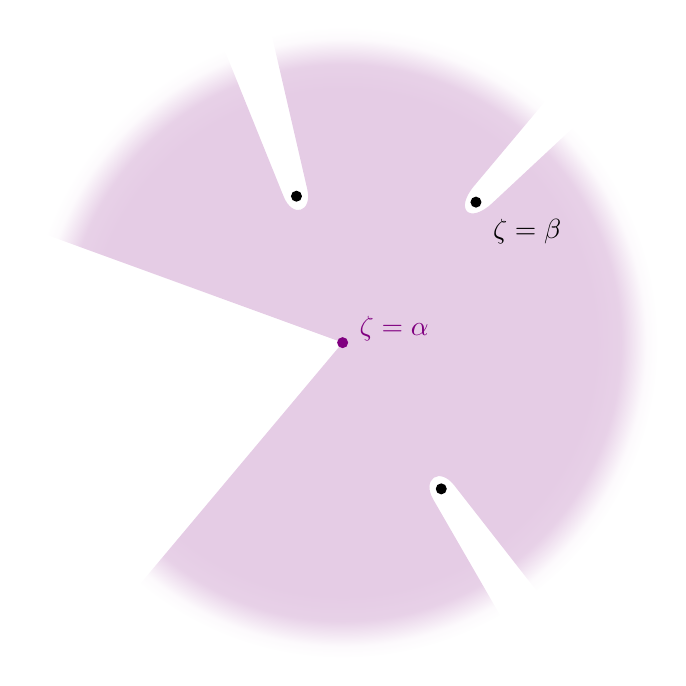
\begin{tikzpicture}
\newcommand{\spill}{4}
\fill[violet!20, bezier bounding box, path fading=radial edge]
  (-\spill, -\spill) (\spill, \spill)
  (0, 0) -- (160:\spill)
  arc (160:112:\spill) -- (112:2) .. controls (112:1.7) and (103:1.7) .. (103:2) -- (103:\spill)
  arc (103:50:\spill) -- (50:2.6) .. controls (50:2.2) and (43:2.2) .. (43:2.6) -- (43:\spill)
  arc (43:-52:\spill) -- (-52:2.3) .. controls (-52:2) and (-60:2) .. (-60:2.3) -- (-60:\spill)
  arc (-60:-130:\spill) -- (0, 0);
\fill[violet] circle (0.7mm) node[anchor=195, outer sep=1mm] {$\zeta = \alpha$};
\node[anchor=north west, outer sep=1mm] at (46.5:2.46) {$\zeta=\beta$};
\foreach \p in {(107.5:1.95), (46.5:2.46), (-56:2.24)} {
  \fill \p circle (0.7mm);
}
\end{tikzpicture}
\caption{The domain $\Omega_\alpha$ \textcolor{orange}{[Revise to show asector]}}\label{Fig:domain}
\end{figure}
\color{Maroon}
\begin{theorem}[restatement of \ref{thm:borel_reg_ODE}]
Choose a root $-\alpha$ of $P$. Choose an open sector $\Omega_\alpha$ which has an opening angle of $\pi$ or less, has $\zeta = \alpha$ at its tip, and doesn't touch any other root of $P(-\zeta)$. Equation~\eqref{eqn:standard ODE} has a unique solution $\Psi_\alpha$ in the affine subspace
\[ z^{-\tau_\alpha} + \dualsingexpalg{-\tau_\alpha-1}(\Omega_\alpha) \]
of the space $\dualsingexpalg{-\tau_\alpha}(\Omega_\alpha)$ from Section~\textcolor{orange}{[figure out where to put definition]}. That solution is Borel regular.
\end{theorem}
The key to our proof is recasting Equation~\eqref{eqn:standard ODE} as an integral equation in the position domain. This integral equation belongs to a well-behaved class of regular singular Volterra equations, which we study in~\cite{reg-sing-volterra}. In particular, it can be solved using Picard iteration, which refines an initial guess toward the unique solution in its basin of attraction. We'll use \textcolor{magenta}{the guess $\frac{1}{\Gamma(\tau_\alpha)} \zeta^{\tau_\alpha - 1}$ [actually, use prototype solution instead]} to find a solution $\psi_\alpha$ with the same singularity at $\zeta_\alpha = 0$.
%%\begin{theorem}[Theorem~4 from \cite{reg-sing-volterra}]\label{thm:sing-soln}
%%The equation $\hat{\mathcal{P}}_\alpha \psi_\alpha = 0$ has a unique solution $\psi_\alpha$ in the affine subspace
%%\[ \zeta_\alpha^{\tau_\alpha-1} + \singexpalg{\tau_\alpha}(\Omega_\alpha) \]
of the space $\singexpalg{\tau_\alpha-1}(\Omega_\alpha)$.
%%\end{theorem}

For the Borel regularity part of the proof, we need to make a connection between the analytic and formal worlds. To do this in the position domain, we again use Picard iteration. \textcolor{orange}{[This does seem to generalize Delabaere's argument! We should confirm and mention that.]}
\begin{lemma}\label{lem:picard-power}
In Theorem~4 of \cite{reg-sing-volterra}, the solution $\psi_\alpha$ can be expressed as the sum of a power series in $\zeta_\alpha^{\tau_\alpha - 1} \C\{\zeta_\alpha\}$.
%%can be expressed as a convergent power series of the form
%%\[ c_1 \zeta_\alpha^{\tau_\alpha - 1} + c_2 \zeta_\alpha^{\tau_\alpha} + c_3 \zeta_\alpha^{\tau_\alpha + 1} + c_4 \zeta_\alpha^{\tau_\alpha + 2} + \ldots. \]
\end{lemma}
\begin{proof}
%%Theorem~\ref{thm:sing-soln} is a corollary of Theorem~\ref{thm:general_volterra} of \cite{reg-sing-volterra}.
The ring of formal power series $\C\{\zeta_\alpha\}$ is isomorphic to the ring of germs of holomorphic functions at $\zeta = \alpha$. This isomorphism identifies the analytic and formal versions of the integration operator $\partial^{-1}_{\zeta, \alpha}$. In the argument that follows, we'll only distinguish the analytic and formal interpretations of $\C\{\zeta_\alpha\}$ when we need to.

For convenience, let $p = P(-\zeta)$ and $q = Q(-\zeta)$. In \cite{reg-sing-volterra}, to prove Theorem~4, we rewrite the equation $\hat{\mathcal{P}}_\alpha \solwhole = 0$ as a regular singular Volterra equation $\solwhole = \volterra^\alpha \solwhole$ that satisfies the conditions of Theorem~3. The operator $\volterra^\alpha$ is the sum of the ``prototypical'' part
%%\[ \hardpart^\alpha = -\tfrac{1}{P(-\zeta)} \circ \partial^{-1}_{\zeta, \alpha} \circ Q(-\zeta) \]
\[ \hardpart^\alpha = -\tfrac{1}{p} \circ \partial^{-1}_{\zeta, \alpha} \circ q \]
and the perturbation
%%\[ \softpart^\alpha = \tfrac{1}{P(-\zeta)} \circ \partial^{-2}_{\zeta, \alpha} \circ R(\partial^{-1}_{\zeta, \alpha}) \]
\[ \softpart^\alpha = \tfrac{1}{p} \circ \partial^{-2}_{\zeta, \alpha} \circ R(\partial^{-1}_{\zeta, \alpha}). \]

Let's run through the proof of Theorem~3, specialized to the case we consider in Theorem~4. First, picking an arbitrary point $b \in \Omega_\alpha$, we show that the {\em prototype solution}
\[ \solproto(a) = \frac{1}{p(a)} \exp\left(-\int_{b}^{a}\frac{q}{p}\;d\zeta\right) \]
satisfies the equation $\solproto = \hardpart^\alpha \solproto$. We then look for a perturbation $\solptb$ that makes $\solwhole = \solproto + \solptb$ a solution of the Volterra equation we're trying to solve. This is equivalent to solving the inhomogeneous equation
\begin{equation}\label{eqn:inhomog-volterra}
\solptb = \softpart^\alpha \solproto + \volterra^\alpha \solptb
\end{equation}

The central idea of the proof is to show that $\solproto$ lies in $\singexpalg{\tau_\alpha - 1}(\Omega_\alpha)$, that $\softpart^\alpha$ maps $\singexpalg{\tau_\alpha - 1}(\Omega_\alpha)$ into $\singexpalg{\tau_\alpha}(\Omega_\alpha)$ \textcolor{orange}{[check]}, and that $\volterra^\alpha$ is a contraction of $\singexp{\tau_\alpha}{\Lambda}(\Omega_\alpha)$ when $\Lambda$ is large enough. It follows, by the Banach fixed point theorem, equation~\eqref{eqn:inhomog-volterra} has a unique solution $\solptb$ in $\singexp{\tau_\alpha}{\Lambda}(\Omega_\alpha)$. More explicitly, we can solve equation~\eqref{eqn:inhomog-volterra} by Picard iteration. Starting with any initial guess $\solptb^{(0)} \in \singexp{\tau_\alpha}{\Lambda}(\Omega_\alpha)$ and defining
\begin{align*}
\solptb^{(1)} & = \volterra^\alpha \solptb^{(0)} \\
\solptb^{(2)} & = \volterra^\alpha \solptb^{(1)} \\
\solptb^{(3)} & = \volterra^\alpha \solptb^{(2)} \\
& \;\;\vdots
\end{align*}
we get a sequence of functions that converges in $\singexp{\tau_\alpha}{\Lambda}(\Omega_\alpha)$ to a solution.

\textcolor{orange}{[\ldots]}

%%Let's recall some notation from the proof. For convenience, we let $p = P(-\zeta)$ and $q = Q(-\zeta)$.

%%For convenience, let $p = P(-\zeta_\alpha)$ and $q = Q(-\zeta_\alpha)$. In \cite{reg-sing-volterra}, we observed that the Volterra operator $\hardpart^\alpha$ with kernel
%%Let $\hardpart^\alpha$ be the Volterra operator with kernel
%%\[ \hardker^\alpha(a,a') = -\frac{q(a')}{p(a)} \]
%%and let $\softpart^\alpha$ be the Volterra operator with kernel
%%\[ \softker^\alpha(a,a') = -\frac{k_R(a,a')}{p(a)}. \]

%%For convenience, let $p = P(-\zeta)$ and $q = Q(-\zeta)$.

%%As we did in the proof of Theorem~\ref{thm:sing-soln} from \cite{reg-sing-volterra}, let

%%\[ \hardker^\alpha(a,a') = -\frac{q(a')}{p(a)}, \]

%%\[ k_R(a,a')=\sum_{j=0}^\infty \frac{R_{j}}{j!} \, \big(\zeta(a)-\zeta(a')\big)^{j+1} . \]

Since $p$ has a simple root at $\zeta = \alpha$, the prototypical part $\hardpart^\alpha$ sends $\C\{\zeta_\alpha\}$ to itself. In fact, for any real number $\sigma$ that's not a negative integer, $\hardpart^\alpha$ maps $\zeta^\sigma \C\{\zeta_\alpha\}$ to itself. Under the same condition on $\sigma$, the operator $R(\partial^{-1}_{\zeta, \alpha})$ is well-defined as a map from $\zeta_\alpha^\sigma \C\{\zeta_\alpha\}$ to itself,\footnote{This is easiest to see from the formal point of view. Multiplication by $R(\zeta)$ sends convergent series to convergent series, and $\partial^{-1}_{\zeta, \alpha}$ acts like multiplication by $\zeta$ followed by the map $\zeta^\rho \mapsto \tfrac{1}{\Gamma(\rho+1)} \zeta^\rho$. A convergent series stays convergent under any operation that leaves its coefficients the same or smaller. \textcolor{orange}{[Discuss convergence of the operator series from the analytic point of view?]}.} so the perturbation can be seen as a map $\softpart^\alpha \maps \zeta_\alpha^\sigma \C\{\zeta_\alpha\} \to \zeta_\alpha^{\sigma + 1} \C\{\zeta_\alpha\}$.

\textcolor{orange}{[\ldots]}

\end{proof}
\begin{lemma}\label{lem:formal-general-volterra}
The equation $\hat{\mathcal{P}}_\alpha \series{\psi}_\alpha = 0$ has a unique formal solution $\series{\psi}_\alpha$ in the affine subspace
\[ \frac{\zeta_\alpha^{\tau_\alpha-1}}{\Gamma(\tau_\alpha)} + \zeta_\alpha^{\tau_\alpha} \C\llbracket \zeta_\alpha \rrbracket \]
of the space $\zeta_\alpha^{\tau_\alpha - 1} \C\llbracket \zeta_\alpha \rrbracket$.
\end{lemma}
\begin{proof}
\textcolor{orange}{[Argument of Loday-Richaud\ldots]}
\end{proof}
\begin{proof}
Let $\hat{\mathcal{P}}_\alpha$ be the Volterra operator defined in Section~4.5 of \cite{reg-sing-volterra}. Take any holomorphic function $\phi$ on $\Omega_\alpha$ with a well-defined Laplace transform $\Phi = \laplace_{\zeta,\alpha}^{\theta} \phi$ \textcolor{magenta}{[choose $\theta$]}. Lemma~2 of \cite{reg-sing-volterra} shows that $\hat{\mathcal{P}}_\alpha \phi = 0$ if and only if $\mathcal{P}\Phi = 0$ \textcolor{magenta}{[the lemma only states one direction; change it before publication to state both directions]}.

As a consequence of Theorem~\ref{thm:sing-soln}, the equation $\hat{\mathcal{P}}_\alpha \psi_\alpha = 0$ has a unique solution $\psi_\alpha$ in the affine subspace
\[ \frac{\zeta^{\tau_\alpha-1}}{\Gamma(\tau_\alpha)} + \singexpalg{\tau_\alpha}(\Omega_\alpha) \]
of the space $\singexpalg{\tau_\alpha-1}(\Omega_\alpha)$. The same is true on any smaller sector created by shaving a sector off each edge of $\Omega_\alpha$. It follows, by the results of Section~\ref{sec:reg-decay} \textcolor{magenta}{[the domain $\Omega_\alpha$ needs to be a sector for this]}, that the equation $\mathcal{P}\Psi_\alpha = 0$ has a unique solution $\Psi_\alpha$ in the affine subspace
\[ z^{-\tau_\alpha} + \dualsingexpalg{-\tau_\alpha-1}(\Omega_\alpha) \]
of the space $\dualsingexpalg{-\tau_\alpha}(\Omega_\alpha)$.

To show that $\Psi_\alpha$ is Borel regular, first observe that by \textcolor{orange}{[Erdelyi \S 1.6---cite in appdendix; to get uniformity, we might need a constant-width strip, rather than a sector]}, the asymptotic expansion $\series{\Psi}_\alpha = \aexp^\theta \Psi_\alpha$ satisfies the same differential equation that $\Psi_\alpha$ does. In addition, the leadeing term of $\series{\Psi}_\alpha$ is $z^{-\tau_\alpha}$. Thus, $\series{\psi}_\alpha = \borel_\zeta \series{\Psi}_\alpha$ satisfies the same intergral equation that $\psi_\alpha$ does, and its leading term is $\frac{1}{\Gamma(\tau_\alpha)} \zeta^{\tau_\alpha - 1}$.
\end{proof}
\color{black}

%As a consequence of Theorem 4 in {\tt reg-volterra} we get 
%
%\begin{theorem}\label{thm1-dim}
%In the previous set-up, there exists a unique solution of $\hat{P}_j\psi_j=0$ with $\zeta_j=\zeta-\alpha_j$ and
%\begin{equation}\label{P-hat_j}
%\hat{P}_j:=P(-\alpha_j-\zeta_j)+\partial_{\zeta,\alpha_j}^{-1}\circ Q(-\alpha_j-\zeta_j)+\partial_{\zeta,\alpha_j}^{-2}\circ\sum_{r=0}^{d-1}R_r(\partial_{\zeta,\alpha_j}^{-1})\circ (-\alpha_j-\zeta_j)^r
%\end{equation}
%such that $\psi_j$ blows up as $\zeta^{\tau_j-1}$ at $\alpha_j$:
%${\psi}_j(\zeta_j)=\zeta_j^{\tau_j-1}+f_j$ and $f_j\in\mathcal{HL}^{\infty,-\tau_j}(\Omega_j)$ with $\Omega_j$.
%\end{theorem}
\begin{theorem}\label{thm2-dim}
%For every $j=1,...,d$ let $\psi_j(\zeta_j)$ be the unique solution of $\hat{P}_j\psi_j=0$ as in in Theorem \ref{thm1-dim}. Then $\psi_j(\zeta_j)$ admits a well defined Laplace transform $\Psi_j:=\laplace_{\zeta_j,-\alpha_j}^{\theta_j}$ for some direction $\theta_j$.
For each root $\alpha$ of $P$, let $\tilde{\Psi}_\alpha(z)=e^{-\alpha z}z^{-\tau_\alpha}\sum_{n=0}^{\infty}a_{\alpha,n}z^{-n}$ be the formal solution of $\mathcal{P}\Psi=0$ with $a_{\alpha,0}=1$. Then $\series{\Psi}_\alpha(z)$ is Borel summable and its Borel sum is proportional to $\Psi_\alpha$. 
\end{theorem}
\begin{proof}
We divide the proof into the following steps:
\begin{itemize}
\item[$(a)$] let $\series{\psi}_\alpha:=\borel_{\zeta}\series{\Psi}_\alpha$, then $\hat{P}_\alpha\series{\psi}_\alpha=0$.
\item[$(b)$] prove that $\laplace_{\zeta,\alpha}^{\theta}\circ\borel_\zeta\series{\Psi}_\alpha\propto \Psi_\alpha $. 
\end{itemize}

Step $(b)$ clearly follows from \cite[Theorem 4]{reg-sing-volterra} and step $(a)$. In fact, $\Tilde{\psi}_\alpha$ and ${\psi}_\alpha$ are both solutions of $\hat{P}_\alpha\psi=0$ and \textcolor{magenta}{by uniqueness}\footnote{\color{magenta} One possibility: show that a solution of a formal Volterra equation of the type we have is determined by the $z^{-\tau_\alpha}$ asymptotics somehow? Not enough in general. Another possibility: [\ldots]} they are proportional in a neighbourhood of $\alpha_j$. Then, we can Laplace transform ${\psi}_\alpha$ along a ray $\Gamma_{\alpha}^\theta$ in $\Omega_\alpha$. Hence if $\hat{\psi}_\alpha$ denotes the analytic continuation of $\tilde{\psi}_\alpha$ which agrees with $\psi_\alpha$, we can Laplace transform $\hat{\psi}_\alpha$ along $\Gamma_{\alpha}^\theta$, too. 

We now prove step $(a)$: we want to show that $\series{\psi}_\alpha=\borel_{\zeta}\series{\Psi}_\alpha$ is a solution of $\hat{\mathcal{P}}_\alpha\series{\psi}_\alpha=0$. Recall that $\tilde{\Psi}_\alpha$ is a trans-series, thus the Borel transform of $z^{-\lambda}\tilde{\Psi}_\alpha$ is written in terms of the convolution product $\ast_{\alpha}$.   

%First notice that if $\series{\Psi}_j=e^{-\alpha_jz}\sum_{n=0}^{\infty}a_{j,n}z^{-n-\tau_j}$ solves $\mathcal{P}\Psi=0$ then $\sum_{n=0}^{\infty}a_{j,n}z^{-n-\tau_j}$ is a solution of $\mathcal{P}_j\Psi=0$ with

%\begin{equation}
%\mathcal{P}_j:=P(-\alpha_j+\partial_z)+\frac{1}{z}Q(-\alpha_j+\partial_z)+\frac{1}{z^2}\sum_{r=0}^dR_r(z^{-1})(-\alpha_j+\partial_z)^r
%\end{equation} 

%Hence 

%\begin{

%Then we take the (formal) Borel transform $\borel_\zeta$ of  $\mathcal{P}_j \sum_{n=0}^{\infty}a_{j,n}z^{-n-\tau_j}$


\begin{align*}
  \borel_{\zeta}\left(\mathcal{P}\series{\Psi}_\alpha\right)&= \left[P(-\zeta)+1\ast_{\alpha} Q(-\zeta)+\zeta \ast_{\alpha} \left(\sum_{r=0}^{d-1}\borel_\zeta(R_r(z^{-1}))\ast_{\alpha}(-\zeta)^r\right)\right]\series{\psi}_\alpha(\zeta_\alpha)\\
  &=\left[P(-\zeta)+\partial_{\zeta,\alpha}^{-1}\circ Q(-\zeta)+\fracderiv{-2}{\zeta}{\alpha} \left(\sum_{r=0}^{d-1}R_r(\fracderiv{-1}{\zeta}{\alpha} )(-\zeta)^r\right)\right]\series{\psi}_\alpha(\zeta_j)\\&=\hat{P}_\alpha\tilde{\psi}_\alpha(\zeta_\alpha)
\end{align*}
%\begin{multline*}
%\borel_\zeta\left(\mathcal{P}\series{\Psi}_j\right)=\borel_\zeta\left[e^{-\alpha_j z}\mathcal{P}_j\sum_{n=0}^{\infty}a_{j,n}z^{-n-\tau_j}\right]=\\
%\left[P(-\alpha_j-\zeta_j)+\partial_{\zeta_j,0}^{-1}\circ Q(-\alpha_j-\zeta_j)+\partial_{\zeta_j,0}^{-2}\circ \sum_{r=0}^dR_r(\partial_{\zeta_j,0}^{-1})\circ (-\alpha_j-\zeta_j)^r\right]\sum_{n=0}^{\infty}\frac{a_{j,n}}{\Gamma(n+\tau_j)}\zeta_j^{n+\tau_j-1}\\
%\left[P(-\zeta)+\partial_{\zeta_j,0}^{-1}\circ Q(-\zeta)+\partial_{\zeta_j,0}^{-2}\circ \sum_{r=0}^dR_r(\partial_{\zeta_j,0}^{-1})\circ (-\zeta)^r\right]\sum_{n=0}^{\infty}\frac{a_{j,n}}{\Gamma(n+\tau_j)}\zeta_j^{n+\tau_j-1}
%\end{multline*}
%where 
%
%\begin{align*}
%\series{\psi}_j(\zeta_j):=\borel\series{\Psi}_j(\zeta_j)&=\borel\left(e^{-\alpha_j z}z^{-\tau_j}\sum_{n=0}^{\infty}a_{j,n}z^{-n}\right)(\zeta_j)=\borel\left(z^{-\tau_j}\sum_{n=0}^{\infty}a_{j,n}z^{-n}\right)(\zeta-\alpha_j)\\
%&=\sum_{n=0}^{\infty}\frac{a_{j,n}}{\Gamma(n+\tau_j)}(\zeta-\alpha_j)^{n+\tau_j-1}
%\end{align*}

Hence, the Borel transform of $\series{\Psi}_\alpha$ is a solution of $\hat{P}_\alpha\series{\psi}_\alpha$=0. 
\end{proof}

%\color{Turquoise}
%\begin{lemma}\label{step a}
%    Let $\hat{\psi}_j$ be the unique solution of $\hat{P}_j\hat{\psi}_j=0$, then it admits a Laplace transform. 
%\end{lemma}

%\begin{proof}
 %   We’ll prove the following: 
  %  \begin{itemize}
   %     \item there are only a finite number of singularities in the Borel plane, hence there is a direction which avoids all the singularities;
    %    \item the analytic continuation of $\hat{\psi}_j$ along that direction grows sub-exponentially. 
    %\end{itemize}
    %The singularities of $\hat{P}_j$ are at $P(-\alpha_j-\zeta_j)=0$, hence at $\zeta_j=\alpha_k-\alpha_j$ for every $k=1,...,d$. In fact, we can prove this statement using a perturbative method that goes back to \'Ecalle (see \cite{EcalleIII}, \cite[Section 2.5]{loday-Remy2011}). Let $\epsilon$ be a parameter and let $f_j(\zeta,\epsilon):=\sum_{k\geq 0}f_{j,k}(\zeta)\epsilon^k$ be a solution of  
   % \[\left[P(-\zeta)+\fracderiv{-1}{\zeta}{\alpha_j}\circ Q(-\zeta)+\epsilon\fracderiv{-2}{\zeta}{\alpha_j}\circ\sum_{r=0}^{d-1}R_r(\fracderiv{-1}{\zeta}{\alpha_j})\circ(-\zeta)^r\right]f_j=0\]
   % \textcolor{red}{such that $f_j(\zeta,1)=\hat{\psi}_j(\zeta)$}. We solve order by order in $\epsilon$: at order zero

    %\begin{align*}
     %   &P(-\zeta)f_{j,0}+\fracderiv{-1}{\zeta}{\alpha_j}\circ Q(-\zeta)f_{j,0}=0\\
      %  &-P'(-\zeta)f_{j,0}+P(-\zeta)\partial_\zeta f_{j,0}+Q(-\zeta)f_{j,0}=0\\
       % &P(-\zeta)\partial_\zeta f_{j,0}=P'(-\zeta)f_{j,0}-Q(-\zeta)f_{j,0}
    %\end{align*}
    %If $\zeta\neq\alpha_k$ for $k=1,...,d$ we can solve the first order equation and for $a\neq\alpha_k$
    %\begin{align*}
     %   f_{j,0}&=f_{j,0}(a)\cdot \exp\left(\int_a^{\zeta}\frac{P'(-t)-Q(-t)}{P(-t)}dt\right)\\
      %  &=f_{j,0}(a)\cdot \frac{P(-a)}{P(-\zeta)}\exp\left(-\int_a^{\zeta}\frac{Q(-t)}{P(-t)}dt\right)
    %\end{align*}
    %Therefore, $f_{j,0}$ is singular at $\zeta=\alpha_k$ for every $k=1,...,d$ (or equivalently, at $\zeta_j=\alpha_k-\alpha_j$). Then, for $n\geq 1$

    %\begin{align*}
     %   \left[P(-\zeta)+\fracderiv{-1}{\zeta}{\alpha_j}\circ Q(-\zeta)\right]f_{j,n}=-\fracderiv{-2}{\zeta}{\alpha_j}\circ\sum_{r=0}^{d-1}R_r(\fracderiv{-1}{\zeta}{\alpha_j})\circ(-\zeta)^r f_{j,n-1}
    %\end{align*}
    %and since $R_r$ is entire, the right-hand side is an infinite sum of the convolution product of an entire function with $f_{j,n-1}$, hence it  has the same singularities as $f_{j,n-1}$ (see Lemma 6.15 \cite{diverg-resurg-i}). Therefore, we deduce $f_{j,1}$ is singular at $\zeta=\alpha_k$ for $k=1,...,d$ and inductively, $f_{j,n}$ is singular at $\zeta=\alpha_k$ for $k=1,...,d$. 

    %Let $\theta$ be the direction that avoids all the singularities, we now prove that the analytic continuation of $\hat{\psi}_j$ grows sub-exponentially. In fact, it is enough to adapt the Gr\"onwall lemma to integral equations (see Lemma 3.9 \cite{diverg-resurg-iii}]). 
   %Let $\Omega$ be the open domain where $\hat{\psi}_j$ is analytic and let $p$ be a point in $\Omega$ such that $\Omega':=\Omega\setminus B_{r}(\alpha_j)$ is star-shaped from $p$ ($B_r(\alpha_j)$ is the ball of radius $r$ and center in $\alpha_j$). By assumption on the coefficients of the ODE \eqref{eqn:standard ODE} 
   %\begin{align*}
    %   a:=\sup_{\zeta\in\Omega'}\frac{|Q|(|\zeta|)}{|P(-\zeta)|}<\infty\, \qquad b:=\sup_{\zeta\in\Omega'}\frac{1}{|P(-\zeta)|}<\infty
   %\end{align*}
   %hence, for every $\zeta\in\Omega'$, writing $\xi=|\zeta|$ and $\zeta=p+\xi e^{i\eta}$
   %\begin{align*}
    %|\hat{\psi}_j(\zeta)|&\leq \frac{1}{|P(-\zeta)|}\left[\int_{|\alpha_j|}^\xi|Q|(\rho) |\hat{\psi}_j(\rho e^{i\theta})|d\rho+\int_{|\alpha_j|}^\xi \sum_{r=0}^{d-1}|\hat{R}_r(\xi-\rho)|\cdot \rho^r |\hat{\psi}_j(\rho e^{i\theta})| d\rho\right]\\
     %  &\leq \frac{1}{|P(-\zeta)|}\left[\int_{|\alpha_j|}^{|p|}+\int_{|p|}^\xi|Q|(\rho) |\hat{\psi}_j(\rho e^{i\theta})|d\rho+\int_{|\alpha_j|}^{|p|}+\int_{|p|}^\xi \sum_{r=0}^{d-1}|\hat{R}_r(\xi-\rho)|\cdot \rho^r |\hat{\psi}_j(\rho e^{i\theta})| d\rho\right]\\
      % &\leq a \int_{|p|}^\xi  |\hat{\psi}_j(\rho e^{i\theta})|d\rho +c \sum_{r=0}^{d-1}\int_{|p|}^\xi|\hat{R}_r(\xi-\rho)|\cdot \rho^r|\hat{\psi}_j(\rho e^{i\theta})| d\rho +\\
      % &\qquad +c\left[\int_{|\alpha_j|}^{|p|}|Q|(\rho) |\hat{\psi}_j(\rho e^{i\theta})|d\rho+\int_{|\alpha_j|}^{|p|} \sum_{r=0}^{d-1}|\hat{R}_r(\xi-\rho)|\cdot \rho^r |\hat{\psi}_j(\rho e^{i\theta})| d\rho\right]\\
      % &\leq a \int_{|p|}^\xi  |\hat{\psi}_j(\rho e^{i\theta})|d\rho +c \sum_{r=0}^{d-1}\int_{|p|}^\xi|\hat{R}_r(\xi-\rho)|\cdot \rho^r|\hat{\psi}_j(\rho e^{i\theta})| d\rho +\\
      % &\qquad + a'\int_{|\alpha_j|}^{|p|}|\hat{\psi}_j(\rho e^{i\theta})|d\rho+ c\sum_{r=0}^{d-1}\int_{|\alpha_j|}^{|p|} |\hat{R}_r(\xi-\rho)|\cdot  \rho^r|\hat{\psi}_j(\rho e^{i\theta})| d\rho%\\
      % %&\leq a \int_{|\alpha_j|}^\xi  |\hat{\psi}_j(\rho e^{i\theta})|d\rho +c  \sum_{r=0}^{d-1} \xi^{r} \int_{|\alpha_j|}^\xi |\hat{R}_r(\xi-\rho)|\cdot|\hat{\psi}_j(\rho e^{i\theta})| d\rho \\
      % %&=a \int_{|p|}^\xi  |\hat{\psi}_j(\rho e^{i\theta})|d\rho +c  \sum_{r=0}^{d-1} \xi^{r} \int_{|p|}^\xi |\hat{R}_r(\xi-\rho)|\cdot|\hat{\psi}_j(\rho e^{i\theta})| d\rho+\\
      % %&\qquad + a \int_{|\alpha_j|}^{|p|}  |\hat{\psi}_j(\rho e^{i\theta})|d\rho +c  \sum_{r=0}^{d-1} \xi^{r} \int_{|\alpha_j|}^{|p|} |\hat{R}_r(\xi-\rho)|\cdot|\hat{\psi}_j(\rho e^{i\theta})| d\rho
   %\end{align*}
   %where $\hat{R}_r=\borel(z^{-2}R_r)$, for every $r=0,...,d-1$. 
   %%For every $r=0,...,d-1$, we define $F_r(z)=R_r(z)$
   %We want to show that for every $m\geq 0$, $|\hat{\psi}_j(\zeta)|<\hat{W}_m(\xi)$ for $\zeta$ on the ray $\zeta=p+\xi e^{i\theta}\in\Omega'$, where $\hat{W}_m$ is the unique solution of 

   %\begin{equation}
    %   \hat{W}=m+a\ast_{|p|}\hat{W}+c\sum_{r=0}^{d-1}\hat{R}_r\ast_{|p|} (-\zeta^r\hat{W})
 %  \end{equation}

 %  \textcolor{red}{Be careful with derivatives: maybe rewrite Lemma 3.8 in such a way that includes them. This means that equation 27 is not anymore algebraic, but it will include terms of the form $R_r(z) \tilde{W}^{(r)}$.
  % There is also another problem, the reasoning of Delabere in Lemma 3.9 requires the existence of a point $p_0$ in $\Omega'$ such that $|\hat{\psi}_j(p_0)|\leq |\hat{W}_m(p_0)|$ for every $m\geq 0$. Can we argue that $|\hat{\psi}_j(\rho e^{i\theta})|$ is bounded for $\rho\in [|\alpha_j|,|p|]$? }
%\end{proof}
\color{violet}
\subsubsection{A new proof of the Borel summability of the Poincar\'{e} solutions}\label{sec:new-summability-proof}
\textcolor{orange}{[Mention that this is a component of the earlier Borel regularity proof.]}
\color{black}
\subsection{Borel regularity for thimble integrals}\label{borel-reg-thimble}

Recall the setting from Section~\ref{borel-reg:explanatory-power}: let $X$ be a $1$-dimensional complex manifold equipped with a volume form $\nu\in\Gamma(X,\Omega^1)$ and a holomorphic function $f\colon X\to\C$ with non--degenerate critical points. Let $I$ be the thimble integral 
\begin{equation}\label{exp-int}
I \defeq \int_{\Lambda_a^\theta} e^{-zf} \nu
\end{equation}
where $\Lambda_a^\theta$ is the thimble through the critical point $a$. In this section, we'll prove that thimble integrals of the form \eqref{exp-int} are Borel regular. The first step will be to rewrite $I$ as the Laplace transform of a function $\iota$ which is explicitly given by the\textit{thimble projection formula}.% \eqref{eqn:formula-proof}.   
\begin{lemma}\label{lem:thimble_proj_formula-proof}
\textcolor{magenta}{[Well-known result---see, e.g., \S 3.3 of \cite{pham}, which uses the variation $\nu/df$ instead of derivative of integral.]} A function $\iota$ with $I = \laplace_{\zeta, \alpha}^\theta \iota$ is given by the {\em thimble projection formula}
\begin{equation}\label{eqn:formula-proof}
    \iota = \frac{\partial}{\partial \zeta} \left( \int_{\Lambda_\alpha^\theta(\zeta)}\nu \right),
\end{equation}
where $\Lambda_\alpha^\theta(\zeta)$ is the part of $\Lambda_a^\theta$ that goes through $f^{-1}([\alpha,\zeta e^{i\theta}])$. Notice that $\Lambda_\alpha^\theta(\zeta)$ starts and ends in $f^{-1}(\zeta)$. \textcolor{magenta}{[The thimble $\Lambda_a^\theta$ needs an orientation, but the orientation is arbitrary.]}
\end{lemma}
\begin{proof}
    Let us recast the integral $I$ into the position domain. As $\zeta$ goes rightward from $\alpha$ with angle $\theta$, the start and end points of $\Lambda_\alpha^\theta(\zeta)$ sweep backward along $\Lambda^-_\alpha(\zeta)$ and forward along $\Lambda^+_\alpha(\zeta)$, respectively. Hence, we have
\begin{align*}
I(z) & = \int_{\Lambda_a^\theta} e^{-zf} \nu \\
& = \int_{\alpha}^{e^{i\theta} \infty} e^{-z\zeta} \left[\frac{\nu}{df}\right]_{\operatorname{start} \Lambda_\alpha^\theta(\zeta)}^{\operatorname{end} \Lambda_\alpha^\theta(\zeta)}\,d\zeta.
\end{align*}
Noticing that the right-hand side is a Laplace transform, we learn that
\begin{equation}\label{thimble-difference}
{\iota}(\zeta) = \left[\frac{\nu}{df}\right]_{\operatorname{start} \Lambda_\alpha^\theta(\zeta)}^{\operatorname{end} \Lambda_\alpha^\theta(\zeta)}.
\end{equation}
\end{proof}
We'll now prove that $I$ is Borel regular:
\begin{theorem}\label{thm:maxim-proof}
If the integral defining $I$ is absolutely convergent, then $I$ is Borel regular. More explicitly: 
\begin{enumerate}
\item\label{part-1} As $z \to \infty$ along the ray $z \in e^{-i\theta}\,\R_{>0}$, the function $I$ is asymptotic to a trans-monomial $\tilde{I}\in e^{-z \alpha} z^{-1/2} \C\llbracket z^{-1}\rrbracket$.
\item\label{part-2} The series $\tilde{I}$ is $1$-Gevrey. In other words, $\tilde{\iota} \defeq \borel_\zeta \tilde{I}$ converges near $\zeta=\alpha$.
\item\label{part-3} If you continue the sum of $\tilde{\iota}$ along the ray $\Gamma_\alpha^\theta$, and take its Laplace transform along that ray, you'll recover $I$.
\end{enumerate}
\end{theorem}
\begin{proof}
Since $f$ has non--degenerate critical points, we can find a holomorphic chart $\tau$ around $a$ with $\tfrac{1}{2} \tau^2 = f - f(a)$. Let $\Lambda^-_\alpha$ and $\Lambda^+_\alpha$ be the parts of $\Lambda_a^\theta$ that go from the past ($-e^{-i\theta}\infty$) to $a$ and from $a$ to the future ($+e^{-i\theta}\infty$), respectively. We can arrange for $\tau$ to be valued in $(-\infty, 0]$ and $[0,\infty)$ on $\Lambda^-_\alpha$ and $\Lambda^+_\alpha$, respectively. \textcolor{magenta}{[Point out that we can always accomplish this by changing the sign of $\tau$.]} Since $\nu$ is holomorphic, we can express it as a Taylor series
\[ \nu = \sum_{m \ge 0} b_m^a \tau^m\,d\tau \]
that converges in some disk $|\tau| < \varepsilon$.

Let's write $\approx$ when two functions are asymptotic at all orders around the base point; by the steepest descent method,\footnote{The details can be found in \cite{miller2006applied}: follow the proof of Proposition~2.1 in through equation~(2.9).}
%%\[ e^{-z\zeta_\alpha} I_\alpha(z) \approx \int_{\tau \in [-\varepsilon, \varepsilon]} e^{-z\tau^2/2} \nu \]
\[ e^{z \alpha} I \approx \int_{\tau \in [-\varepsilon, \varepsilon]} e^{-z\tau^2/2} \nu \]
as $z \to \infty$. Plugging in the Taylor series for $\nu$, we get
\begin{align*}
e^{z \alpha} I & \approx \int_{-\varepsilon}^\varepsilon e^{-z\tau^2/2} \sum_{m \ge 0} b_m^a \tau^m\,d\tau \\
& = \int_{-\varepsilon}^\varepsilon e^{-z\tau^2/2} \sum_{n \ge 0} b_{2n}^a \tau^{2n}\,d\tau.
\end{align*}
By the dominated convergence theorem,\footnote{Notice that the sum over $k$ is empty when $n = 0$. Following convention, we extend the double factorial to all odd integers by its recurrence relation, giving $(-1)!! = 1$.}
\begin{align*}
e^{z \alpha} I & \approx \sum_{n \ge 0} b_{2n}^a \int_{-\varepsilon}^\varepsilon e^{-z\tau^2/2} \tau^{2n}\,d\tau \\
& = \sum_{n \ge 0} (2n-1)!!\,b_{2n}^a \left[ \sqrt{2\pi}\,z^{-(n+1/2)} \operatorname{erf}\big(\varepsilon \sqrt{z/2}\big) - 2e^{-z\varepsilon^2/2} \sum_{\substack{k \in \mathbb{N}_+ \\ k \le n}} \frac{\varepsilon^{2k-1}}{(2k-1)!!} z^{-n+k-1} \right].
\end{align*}

The annoying $e^{-z\varepsilon^2/2}$ correction terms are crucial for the convergence of the sum, but we can get rid of them and still have a formal series asymptotic to $e^{-z \alpha} I(z)$. In other words,
\[ e^{z \alpha} I(z) \sim \sqrt{2\pi} \sum_{n \ge 0} (2n-1)!!\,b_{2n}^a\,z^{-(n+1/2)} \operatorname{erf}\big(\varepsilon \sqrt{z/2}\big). \]
To see why, cut the sum off after $N$ terms, and observe that
\begin{align*}
  \Bigg | \sum_{n= 0}^N(2n-1)!! b_{2n}^a  2e^{-z\varepsilon^2/2} \sum_{\substack{k \in \mathbb{N}_+ \\ k \le n}} \frac{\varepsilon^{2k-1}}{(2k-1)!!} z^{-n+k-1} \Bigg | &\leq  2 e^{-\Re (z) \varepsilon^2/2} \sum_{n=0}^N(2n-1)!! b_{2n}^a n|z|^{-n}.
\end{align*}
The right-hand side goes to $0$ as $\Re(z)$ grows.
%Hence,
%\[ e^{-z\zeta_\alpha} I_\alpha(z) \sim \sqrt{2\pi} \sum_{n \ge 0} (2n-1)!!\,b_{2n}^\alpha\,z^{-(n+1/2)} \operatorname{erf}\big(\varepsilon \sqrt{z/2}\big). \]
The differences $1 - \operatorname{erf}\big(\varepsilon \sqrt{z/2}\big)$ shrink exponentially as $z$ grows \cite[inequality~(5)]{chiani-dardari-book}, allowing the simpler estimate
\[ e^{z\alpha} I(z) \sim \sqrt{2\pi} \sum_{n \ge 0} (2n-1)!!\, b_{2n}^a \,z^{-(n+1/2)}. \]
Hence, defining the formal series $\tilde{I}$
\[\tilde{I}(z):=e^{-z\alpha} z^{-1/2}\, \sqrt{2\pi} \sum_{n \ge 0} (2n-1)!!\, b_{2n}^a \,z^{-n}\]
we get $\tilde{I}\in e^{-z\alpha}z^{-1/2}\C\llbracket z^{-1}\rrbracket$. This ends the proof of part \ref{part-1}.

Using the porperties of the Borel tranform acting on trans-mononials \ref{sec:action_transseries} we get 
\begin{align*}
\tilde{\iota} & = \sqrt{2\pi} \sum_{n \ge 0} (2n - 1)!! \,b_{2n}^a\,\frac{\zeta_\alpha^{n+\tfrac{1}{2}}}{\Gamma(n+\tfrac{1}{2})} \\
&= \sqrt{2\pi} \sum_{n \ge 0} \frac{2^n}{\sqrt{\pi}} \,b_{2n}^a\,\zeta_\alpha^{n+\tfrac{1}{2}}
\end{align*}
We know from the definition of $\varepsilon$ that $\left|b_n^a\right| \varepsilon^n \lesssim 1$, thus we deduce that $\tilde{\iota}$ has a finite radius of convergence. This ends the proof of part \ref{part-2}. %$|a_{j,n}| \lesssim \left(\tfrac{2}{\varepsilon^2}\right)^n\,n!\,$, showing that $\tilde{I}_j$ is $1$-Gevrey.

\textcolor{RoyalBlue}{[Analytic/position version starts here.]} The proof of part \ref{part-3} relies on the thimble projection formula \eqref{eqn:formula-proof}; \textcolor{pink}{in fact, we'll show that the Taylor expansion of $\iota$ near $\zeta=\alpha$ agrees with $\tilde{\iota}$.}

We can rewrite the Taylor series for $\nu$ as
\begin{align*}
\nu & = \sum_{n \ge 0} b_n^a [2(f - \alpha)]^{(n - 1)/2}\,df,
\end{align*}
taking the positive branch of the square root on $\Lambda^+_a$ and the negative branch on $\Lambda^-_a$. Plugging this into our expression for $\iota$ (in Theorem \ref{lem:thimble_proj_formula-proof}), we learn that
\begin{align*}
\iota & = \left[ \sum_{m \ge 0} b_m^a [2(f - \alpha)]^{(m - 1)/2} \right]_{\operatorname{start} \Lambda_a(\zeta)}^{\operatorname{end} \Lambda_a(\zeta)} \\
& = \sum_{m \ge 0} b_m^a \Big( [2\zeta_\alpha]^{(m - 1)/2} - (-1)^{m-1}[2\zeta_\alpha]^{(m - 1)/2} \Big) \\
& = \sum_{n \ge 0} 2 b_{2n}^a [2\zeta_\alpha]^{n - 1/2} \\
& = \sum_{n \ge 0} 2^{n+1/2} b_{2n}^a \zeta_\alpha^{n - 1/2}
\end{align*}
In particular, $\tilde{\iota}$ can be analytically continued along $\Gamma_\alpha^\theta$ and its sum is given by $\iota$. %Thus, we can take the Laplace transform of $\phi_j$ and we find
%\begin{align*}
 %   \laplace_{\zeta,\alpha_j}^\theta \phi_j &= \laplace_{\zeta,\alpha_j}^\theta \fracderiv{-1/2}{\zeta}{\alpha_j} \iota_j \\
 %   &= z^{-1/2} \laplace_{\zeta,\alpha_j}^\theta  \iota_j \\
 %   &= z^{-1/2} I_j
%\end{align*}

\color{RoyalBlue}
Lemma~\ref{lem:thimble_proj_formula-proof} tells us that
\begin{align*}
I_j & = \laplace_{\zeta, \alpha_j}^\theta \iota_j \\
e^{z\alpha_j} I_j & = \laplace_{\zeta_j, 0}^\theta \iota_j \\
& = \laplace_{\zeta_j, 0}^\theta \left( \sum_{n = 0}^N 2^{n+1/2} b_{2n}^j \zeta_j^{n - 1/2} + \textcolor{orange}{\zeta^{N+1/2} f}\right) \\
& \color{magenta} = \laplace_{\zeta_j, 0}^\theta \left( \sum_{n = 0}^\infty 2^{n+1/2} b_{2n}^j \zeta_j^{n - 1/2} \right).
%%& = \int_{\Gamma_j^\theta} e^{-z\zeta_j} \iota_j\,d\zeta_j \\
%%& = \int_{\Gamma_j^\theta} e^{-z\zeta_j} \left( \sum_{n \ge 0} 2^{n+1/2} b_{2n}^j \zeta_j^{n - 1/2} \right) d\zeta_j
\end{align*}
Over any finite number of terms, we can exchange the sum with the Laplace transform, giving
\begin{align*}
e^{z\alpha_j} I_j & = \Delta_n + \sum_{n = 0}^N 2^{n+1/2} b_{2n}^j\,\laplace_{\zeta_j, 0}^\theta \zeta_j^{n - 1/2} \\
& = \Delta_n + \sum_{n = 0}^N 2^{n+1/2} b_{2n}^j \Gamma(n + \tfrac{1}{2})\,z^{-n - 1/2} \\
& = \Delta_n + \sum_{n = 0}^N \sqrt{2\pi}\,(2n - 1)!!\,b_{2n}^j\,z^{-n - 1/2},
\end{align*}
where
\[ \Delta_n = \laplace_{\zeta_j, 0}^\theta \left( \sum_{n = N+1}^\infty 2^{n+1/2} b_{2n}^j \zeta_j^{n - 1/2} \right). \]
\begin{verify}
\begin{align*}
2^n \Gamma(n + \tfrac{1}{2}) & = \sqrt{\pi}\,(2n - 1)!! \\
2^{n + 1/2} \Gamma(n + \tfrac{1}{2}) & = \sqrt{2\pi}\,(2n - 1)!!
\end{align*}
\end{verify}

\begin{prop}
Consider a function
\[ \varphi = \sum_{\kappa \in K} a_\kappa \zeta^\kappa \]
defined by a power series with real exponents $K \subset (-1, \infty)$, with a positive lower bound on the distances between the exponents. If the series converges throughout the disk $|\zeta| < \varepsilon$, then
\[ \partial_{\zeta, 0}^{-\nu} \varphi = \sum_{\kappa \in K} \tfrac{\Gamma(\kappa+1)}{\Gamma(\kappa+\nu+1)} \zeta^{\kappa + \nu} \]
on that disk.
\end{prop}
\begin{proof}
The convergence of the series for $\varphi$ in the disk $|\zeta| < \varepsilon$ implies that for each $\eta \in (0, \varepsilon)$, we have $|a_\kappa| \lesssim \eta^{-\kappa}$ over all $\kappa \in K$. The
\end{proof}
\begin{verify}
Reference for monomials: ``Evaluation of Fractional Integrals and Derivatives of Elementary Functions''

For convenience, think of $K$ as sequence, in increasing order. At any point $\zeta = \rho$ with $|\rho| < \varepsilon$, the series defining $\varphi$ converges, implying that
\begin{align*}
& \lim_{\kappa \in K} |a_\kappa \rho^\kappa| = 0 \\
& \lim_{\kappa \in K} |a_\kappa| |\rho|^\kappa = 0 \\
& |a_\kappa| |\rho|^\kappa \lesssim 1 \text{ over all } \kappa \in K \\
& |a_\kappa| \lesssim |\rho|^{-\kappa} \text{ over all } \kappa \in K.
\end{align*}
In other words, for every $r \in (0, \varepsilon)$, we have $|a_\kappa| \lesssim r^{-\kappa}$ over all $\kappa in K$.

Hence, on the region $|\zeta| < |\rho|$, we have
\begin{align*}
|\varphi| & \le \sum_{\kappa \in K} |a_n| |\zeta|^\kappa \\
& \lesssim \sum_{\kappa \in K} r^{-\kappa} |\zeta|^\kappa \\
& = \sum_{\kappa \in K} |\zeta/r|^\kappa.
\end{align*}
In the disk $|\zeta| < r$, the ratio $|\zeta/r|$ is smaller than $1$, so increasing its exponent always decreases the value.

Let $c > 0$ be the lower bound on the distances between the exponents. Choose some $\lambda \in (-1, \infty)$ so that $K \subset (\lambda, \infty)$. For each $n \in \mathbb{N}_{\ge 0}$, the $n$th element of $K$ must be greater than $\lambda + nc$, so
\begin{align*}
|\varphi| & \lesssim \sum_{n = 0}^\infty |\zeta/r|^{\lambda + nc} \\
& = |\zeta/r|^\lambda \sum_{n = 0}^\infty (|\zeta/r|^c)^n \\
& = \frac{|\zeta/r|^\lambda}{1 - |\zeta/r|^c} \\
& = \frac{1}{|\zeta/\rho| - |\zeta/r|^{1+c}}.
\end{align*}
We now see that the series defining $\varphi$ converges absolutely on $|\zeta| < |\rho|$.

The kernel of $\partial_{\zeta, 0}^{\nu-1}$ is $\big(\zeta(p) - \zeta\big)^{\nu-1}$. It has an integrable singularity at $p$, and it's non-singular at $\zeta = 0$.
\end{verify}

\begin{prop}
Suppose $f_0, f_1, f_2, \ldots$ is a sequence of holomorphic functions on some connected domain $\Omega$, and the series $\sum_{k=0}^\infty |f_k|$ converges at each point in $\Omega$. Then, for any $\nu > 0$,
\[ \partial_{\zeta, \alpha}^{-\nu} \left( \sum_{k=0}^\infty f_k \right) = \sum_{k=0}^\infty \partial_{\zeta, \alpha}^{-\nu} f_k \]
throughout $\Omega$.
\end{prop}
\begin{proof}
Given any point $p \in \Omega$, choose a path $\gamma$ that runs through $\Omega$ from $\zeta = \alpha$ to $p$. Since $\gamma$ is the continous image of a closed interval, it's compact, so $\zeta$ is bounded

Recalling that
\[ [\partial^{\nu-1}_{\zeta, \alpha} f](p) \defeq \frac{1}{\Gamma(1-\nu)} \int_{\zeta = \alpha}^p \big(\zeta(p)-\zeta\big)^{-\nu} f\,d\zeta, \]
\textcolor{orange}{[\ldots]}
\end{proof}

By the steepest descent method,\footnote{The details can be found in \cite{miller2006applied}: follow the proof of Proposition~2.1 in through equation~(2.9).} \textcolor{magenta}{[define $\approx$]}
%%\[ e^{-z\zeta_\alpha} I_\alpha(z) \approx \int_{\tau \in [-\varepsilon, \varepsilon]} e^{-z\tau^2/2} \nu \]
\[ e^{z \alpha_j} I_j \approx \int_{\tau \in [-\varepsilon, \varepsilon]} e^{-z\tau^2/2} \nu \]
as $z \to \infty$ along the ray $e^{-i\theta}\, \R_{> 0}$.
%%Since the Taylor series for $\nu$ converges in the disk $|\tau| < \varepsilon$, we know that $|b_m^j| \lesssim \varepsilon^{-m}$ over all $m \ge 0$, giving
%%\[ \left| e^{-z\zeta_j}\;2^{n+1/2} b_{2n}^j \zeta_j^{n - 1/2} \right| \lesssim 2^{n+1/2} \varepsilon^{-2n} e^{-\Re(z\zeta_j)} |\zeta_j|^{n - 1/2}. \]
%%When $z\zeta_j \in \R_{> 0}$, that implies
%%\begin{align*}
%%\left| e^{-z\zeta_j}\;2^{n+1/2} b_{2n}^j \zeta_j^{n - 1/2} \right| \lesssim 2^{n+1/2} \varepsilon^{-2n} e^{-|z||\zeta_j|} |\zeta_j|^{n - 1/2}.
%%\end{align*}
\color{black}
\end{proof}
\begin{remark}\label{rmk:1/2-deriv}
    \textcolor{orange}{[Spirit of the remark: if you want to run the argument above for $\Phi$, you can, but there's one subtlety you should be aware of\ldots]} For some applications, it might be more convenient to study Borel regularity of $\Phi=z^{-1/2}I$, as its asymptotics won't have fractional power singularities. The proof follows the same argument we chose for $I$, but there's one subtulty to be aware of when rewriting $\Phi$ as the Laplace transform of a function $\phi$. Indeed, first notice that \[\phi = \fracderiv{-1/2}{\zeta}{\alpha} \, \iota \]
    Then, we can take the $1/2$ fractional integral on both sides:
    \begin{align*}
        \fracderiv{-1/2}{\zeta}{\alpha} \phi &= \fracderiv{-1}{\zeta}{\alpha} \, \iota \\
        & = \fracderiv{-1}{\zeta}{\alpha} \partial_\zeta \left( \int_{\Lambda_a^\theta(\zeta)}\nu \right) \\
        & = \int_{\Lambda_\alpha^\theta(\zeta)}\nu - \int_{\Lambda_\alpha^\theta(\alpha)}\nu.
    \end{align*}
    The second term vanishes because $\Lambda_\alpha^\theta(\alpha)$ is a single point, leaving
    \[ \fracderiv{-1/2}{\zeta}{\alpha} \phi = \int_{\Lambda_\alpha^\theta(\zeta)}\nu. \]
    Finally, we apply the $1/2$ derivative of both sides, recalling that it's a left inverse of the $1/2$ integral:
    \begin{equation}\label{eqn:formula--1/2}\phi= \fracderiv{1/2}{\zeta}{\alpha} \left( \int_{\Lambda_\alpha^\theta(\zeta)}\nu \right).\end{equation}
    \textcolor{orange}{[This argument works for any function that vanishes at $\alpha$, so maybe we should instead prove it generally in the section on fractional calculus.]}
\end{remark}


\color{RoyalBlue}
The saddle point approximation\footnote{When $f$ is a polynomial see \cite{Malgrange22,pham}. More generally, if $f$ is holomorphic \textcolor{orange}{see \cite{Pham83}?}} gives the formal series 
\begin{equation}
{I}_{j}(z)\sim \tilde{I}_{j}\defeq e^{-z\alpha_j}(2\pi)^{1/2} z^{-1/2}\sum_{n\geq 0}a_{j,n}z^{-n} \qquad \text{ as } \Re z\to \infty. 
\end{equation}
%
Then our main result states that for every $j=1,\ldots,d$, the thimble integral $I_j$ is Borel regular:
\begin{theorem}\label{thm:maxim-dim} Let $\tilde{\Phi}_{j}(z)=z^{1/2}\,\tilde{I}_j(z)\in e^{-z\alpha_j}\C\llbracket z^{-1}\rrbracket$. Then:
\begin{enumerate}
\item\label{int:series-gevrey} The series $\tilde{\Phi}_j$ is $1$-Gevrey, thus $\series{\phi}_j(\zeta)\defeq\borel_\zeta(\tilde{\Phi}_j)$ converges near $\zeta=\alpha_j$
\item\label{int:resum-valid} If you continue the sum of $\tilde{\phi}_j$ along the ray going rightward from $\alpha_j$, and take its Laplace transform along that ray, you'll recover $z^{1/2} I_j$.
\item\label{int:deriv-formula} For any $\zeta$ on the ray going rightward from $\alpha_j$, we have
\begin{multline}\label{formula1}
\hat{\phi}_{j}(\zeta)=\fracderiv{{3/2}}{\zeta} {\alpha_j} \left( \int_{\Lambda_j(\zeta)}\nu \right)=\left(\tfrac{\partial}{\partial \zeta}\right)^2\,\frac{1}{\Gamma\big(\tfrac{1}{2}\big)} \int_{\alpha_j}^\zeta (\zeta-\zeta')^{-1/2} \left( \int_{\Lambda_j(\zeta')} \nu \right)\,d\zeta',
\end{multline}
where $\Lambda_j(\zeta)$ is the part of $\Lambda_j$ that goes through $f^{-1}([\alpha_j, \zeta])$. Notice that $\Lambda_j(\zeta)$ starts and ends in $f^{-1}(\zeta)$. \textcolor{magenta}{[The thimble $\Lambda_j$ needs an orientation, but the orientation is arbitrary.]}
\end{enumerate}
\end{theorem}

\begin{proof}

Part~\eqref{int:series-gevrey}: Let's write $\approx$ when two functions are asymptotic (at all orders around the base point \textbf{[is this the right condition?]}), and $\sim$ when a function is asymptotic to a formal power series (at the truncation order of each partial sum).

Since $f$ has non--degenerate critical points, we can find a holomorphic chart $\tau$ around $a_j$ with $\tfrac{1}{2} \tau^2 = f - f(a_j)$. Let $\Lambda^-_j$ and $\Lambda^+_j$ be the parts of $\Lambda_j$ that go from the past to $a_j$ and from $a_j$ to the future, respectively. We can arrange for $\tau$ to be valued in $(-\infty, 0]$ and $[0, \infty)$ on $\Lambda^-_j$ and $\Lambda^+_j$, respectively. \textcolor{magenta}{[Point out that we can always accomplish this by changing the sign of $\tau$.]} Since $\nu$ is holomorphic, we can express it as a Taylor series
\[ \nu = \sum_{n \ge 0} b_n^j \tau^n\,d\tau \]
that converges in some disk $|\tau| < \varepsilon$.

By the steepest descent method,
%%\[ e^{-z\zeta_\alpha} I_\alpha(z) \approx \int_{\tau \in [-\varepsilon, \varepsilon]} e^{-z\tau^2/2} \nu \]
\[ e^{\textcolor{magenta}{+}z \alpha_j} I_j(z) \approx \int_{\tau \in [-\varepsilon, \varepsilon]} e^{-z\tau^2/2} \nu \]
as $\Re z \to \infty$ (see, for example, \cite[Proposition 2.1]{miller2006applied}---the argument through equation~(2.9)). Plugging in the Taylor series above, we get
\begin{align*}
e^{-z f(\alpha_j)} I_j(z) & \approx \int_{-\varepsilon}^\varepsilon e^{-z\tau^2/2} \sum_{n \ge 0} b_n^j \tau^n\,d\tau \\
& = \int_{-\varepsilon}^\varepsilon e^{-z\tau^2/2} \sum_{n \ge 0} b_{2n}^j \tau^{2n}\,d\tau.
\end{align*}
By the dominated convergence theorem,\footnote{Notice that the sum over $k$ is empty when $n = 0$. Following convention, we extend the double factorial to all odd integers by its recurrence relation, giving $(-1)!! = 1$.}
\begin{align*}
e^{-z f(\alpha_j)} I_j(z) & \approx \sum_{n \ge 0} b_{2n}^j \int_{-\varepsilon}^\varepsilon e^{-z\tau^2/2} \tau^{2n}\,d\tau \\
& = \sum_{n \ge 0} (2n-1)!!\,b_{2n}^j \left[ \sqrt{2\pi}\,z^{-(n+1/2)} \operatorname{erf}\big(\varepsilon \sqrt{z/2}\big) - 2e^{-z\varepsilon^2/2} \sum_{\substack{k \in \mathbb{N}_+ \\ k \le n}} \frac{\varepsilon^{2k-1}}{(2k-1)!!} z^{-n+k-1} \right].
\end{align*}

The annoying $e^{-z\varepsilon^2/2}$ correction terms are crucial for the convergence of the sum, but we can get rid of them and still have a formal series asymptotic to $e^{-z \alpha_j} I_j(z)$. In other words,
\[ e^{-z \alpha_j} I_j(z) \sim \sqrt{2\pi} \sum_{n \ge 0} (2n-1)!!\,b_{2n}^j\,z^{-(n+1/2)} \operatorname{erf}\big(\varepsilon \sqrt{z/2}\big). \]
To see why, cut the sum off after $N$ terms, and observe that
\begin{align*}
  \Bigg | \sum_{n= 0}^N(2n-1)!! b_{2n}^j  2e^{-z\varepsilon^2/2} \sum_{\substack{k \in \mathbb{N}_+ \\ k \le n}} \frac{\varepsilon^{2k-1}}{(2k-1)!!} z^{-n+k-1} \Bigg | &\leq  2 e^{-\Re (z) \varepsilon^2/2} \sum_{n=0}^N(2n-1)!! b_{2n}^j n|z|^{-n}.
\end{align*}
The right-hand side goes to $0$ as $\Re(z)$ grows.
%Hence,
%\[ e^{-z\zeta_\alpha} I_\alpha(z) \sim \sqrt{2\pi} \sum_{n \ge 0} (2n-1)!!\,b_{2n}^\alpha\,z^{-(n+1/2)} \operatorname{erf}\big(\varepsilon \sqrt{z/2}\big). \]
The differences $1 - \operatorname{erf}\big(\varepsilon \sqrt{z/2}\big)$ shrink exponentially as $z$ grows \cite[inequality~(5)]{chiani-dardari-book}, allowing the simpler estimate
\[ e^{-z\alpha_j)} I_j(z) \sim \sqrt{2\pi} \sum_{n \ge 0} (2n-1)!!\, b_{2n}^j \,z^{-(n+1/2)}. \] 

Call the right-hand side $\tilde{I}_j$. We now see that $a_{j,n} = (2n-1)!!\,b_{2n}^j$ in the statement of the theorem. %\textbf{[Resolve discrepancy with previous calculation.]} 

Note that 
\begin{align*}
\borel_{\zeta} \tilde{I}_j & = \sqrt{2\pi} \sum_{n \ge 0} \frac{2^n}{\sqrt{\pi}} \Gamma\big(n+\tfrac{1}{2}\big)\,b_{2n}^j\,\frac{\zeta_j^{n-1/2}}{\Gamma\big(n+\tfrac{1}{2}\big)} \\
& = \sum_{n \ge 0} 2^{n+1/2}\,b_{2n}^j \,\zeta_j^{n-1/2}.
\end{align*}

We know from the definition of $\varepsilon$ that $\left|b_n^j\right| \varepsilon^n \lesssim 1$. Recalling that $(2n - 1)!! \approx (\pi n)^{-1/2}\,2^n\,n!$ as $n \to \infty$, we deduce that $|a_{j,n}| \lesssim \left(\tfrac{2}{\varepsilon^2}\right)^n\,n!\,$, showing that $\tilde{I}_j$ is $1$-Gevrey.

Part~\eqref{int:resum-valid}: Let us recast the integral $I_j$ into the $f$ plane. As $\zeta$ goes rightward from $\alpha_j$, the start and end points of $\Lambda_j(\zeta)$ sweep backward along $\Lambda^-_j(\zeta)$ and forward along $\Lambda^+_j(\zeta)$, respectively. Hence, we have
\begin{align*}
I_j(z) & = \int_{\Lambda_j} e^{-zf} \nu \\
& = \int_{\alpha_j}^\infty e^{-z\zeta} \left[\frac{\nu}{df}\right]_{\operatorname{start} \Lambda_j(\zeta)}^{\operatorname{end} \Lambda_j(\zeta)}\,d\zeta.
\end{align*}
Noticing that the right-hand side is a Laplace transform, we learn that
\begin{equation}\label{thimble-difference}
\hat{\iota}_j(\zeta) = \left[\frac{\nu}{df}\right]_{\operatorname{start} \Lambda_j(\zeta)}^{\operatorname{end} \Lambda_j(\zeta)}.
\end{equation}
%\color{Aquamarine}
%In \'Ecalle's formalism, $\frac{\nu}{df}$ and $\hat{\iota}_j$ are a major and a minor of the singularity $\overset{\triangledown}{I}_\alpha$. [Can we say: $\frac{\nu}{df}$ is a major representing the singularity $\overset{\triangledown}{I}_\alpha$? Or something even simpler?]
%\color{black}

We can rewrite our Taylor series for $\nu$ as
\begin{align*}
\nu & = \sum_{n \ge 0} b_n^j [2(f - f(a_j))]^{n/2}\,\frac{df}{[2(f - f(a_j))]^{1/2}} \\
& = \sum_{n \ge 0} b_n^j [2(f - f(a_j))]^{(n - 1)/2}\,df,
\end{align*}
taking the positive branch of the square root on $\Lambda^+_j$ and the negative branch on $\Lambda^-_j$. Plugging this into our expression for $\hat{\iota}_j$, we learn that
\begin{align*}
\hat{\iota}_j(\zeta) & = \left[ \sum_{n \ge 0} b_n^j [2(f - f(a_j))]^{(n - 1)/2} \right]_{\operatorname{start} \Lambda_j(\zeta)}^{\operatorname{end} \Lambda_j(\zeta)} \\
& = \sum_{n \ge 0} b_n^j \Big( [2\zeta_j]^{(n - 1)/2} - (-1)^{n-1}[2\zeta_j]^{(n - 1)/2} \Big) \\
& = \sum_{n \ge 0} 2 b_{2n}^j [2\zeta_j]^{n - 1/2} \\
& = \sum_{n \ge 0} 2^{n+1/2} b_{2n}^j \zeta_j^{n - 1/2} \\
& = \borel_{\zeta} \tilde{I}_j.
\end{align*}

We have now shown that the sum of $\borel_{\zeta} \tilde{I}_j$ is actually equal to $\hat{\iota}_j$.

%Let $\tilde{\Phi}_j\in\C[\![z^{-1}]\!]$ be such that $\tilde{I}_j(z)=e^{-z\alpha_j}z^{-1/2}\tilde{\Phi}_j(z)$,  
By the action of $\borel_\zeta$ on transseries (Section \ref{sec:action_transseries}) and the properties of convolution (Section \ref{convolution}) we know 
\begin{align*}
\borel_{\zeta} \tilde{I}_j & = \borel_{\zeta}( z^{-1/2} \tilde{\Phi}_j) \\
&=\borel_\zeta z^{-1/2}\ast_{\alpha_j}\borel_\zeta\tilde{\Phi}_j\\
& = \fracderiv{-1/2}{\zeta}{\alpha_j}  \tilde{\phi}_j \\
%& = \partial^{-1/2}_{\zeta \text{ from } \zeta_\alpha} \hat{\varphi}_\alpha.
\end{align*}
It follows, from our conclusion above, that
\begin{equation}\label{shifted-resum-valid}
\hat{\iota}_j(\zeta) = \fracderiv{-1/2}{\zeta}{\alpha_j} \hat{\phi}_j.
\end{equation}
Taking the Laplace transform of both sides and applying properties of the Borel transform (see Proposition~\ref{prop:frac-der-int-borel}), we see that
\begin{align*}
I_j(z) & = \laplace_{\zeta, \alpha_j} \left[ \partial^{-1/2}_{\zeta, \alpha_j}  \hat{\phi}_j \right] \\
& = z^{-1/2} \laplace_{\zeta, \alpha_j} \tilde{\phi}_j,
\end{align*}
as we claimed. 

Part~\eqref{int:deriv-formula}: Since fractional integrals form a semigroup, equation~\eqref{shifted-resum-valid} implies that
\[ \fracderiv{-1}{\zeta}{\alpha_j} \hat{\iota}_j(\zeta) = \fracderiv{-3/2}{\zeta}{\alpha_j} \hat{\phi}_j. \]

Rewriting equation~\eqref{thimble-difference} as
\[ \hat{\iota}_j(\zeta) = \partial_\zeta \left( \int_{\Lambda_j(\zeta)} \nu \right), \]
we can see that
\[ \fracderiv{-1}{\zeta}{\alpha_j} \hat{\iota}_j(\zeta) = \int_{\Lambda_j(\zeta)} \nu - \int_{\Lambda_j(\alpha_j)} \nu. \]
The initial value term vanishes because the path $\alpha_j$ is a point. Hence,
\[ \int_{\Lambda_j(\zeta)} \nu = \fracderiv{-3/2}{\zeta}{\alpha_j} \hat{\phi}_j(\zeta). \]
Recalling that the Riemann-Liouville fractional derivative is a left inverse of the fractional integral, we conclude that
\[ \fracderiv{3/2}{\zeta}{\alpha_j} \left( \int_{\Lambda_j(\zeta)} \nu \right) = \hat{\phi}_j(\zeta). \]
\end{proof}
\color{black}
\begin{remark}
We can use the $1/2$ derivative formula~\eqref{eqn:formula--1/2} to see that the functions $\phi$ are all resurgent, in the sense of \'{E}calle~\cite[\textcolor{orange}{section?}]{EcalleI}. Let's say $\Gamma_\alpha^\theta(\beta)$ is the straight path from $\zeta = \alpha$ to $\zeta = \beta$ in $\C$. As long as this path avoids the critical values of $f$, it lifts uniquely along $f$ to a path $\Lambda_\alpha^\theta(\beta)$ in $X$. This lets us analytically continue $\int_{\Lambda_\alpha^\theta(\zeta)} \nu$ to a star-shaped domain $\Omega_\alpha \subset \C$. Intuitively, $\Omega_\alpha$ is constructed by drawing rays from $\zeta = \alpha$ through all of the other critical values, and then cutting $\C$ along the parts of those rays that go from the other critical values to $\infty$ (see Figure~\ref{Fig:slit domain}).
\begin{figure}
\center
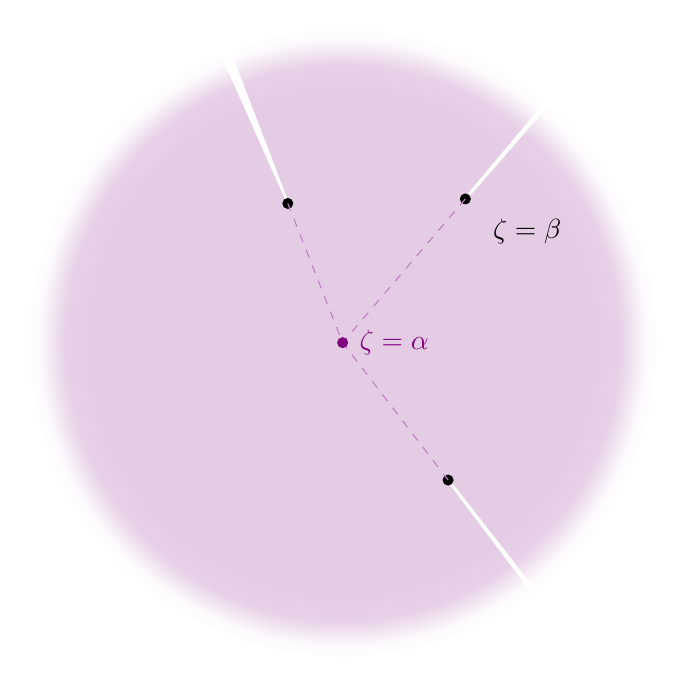
\begin{tikzpicture}
\newcommand{\spill}{4}
\fill[violet!20, bezier bounding box, path fading=radial edge]
  (-\spill, -\spill) (\spill, \spill)
  (0, 0) -- (180:\spill)
  arc (180:113:\spill) -- (112:2) .. controls (112:1.7) and (111:1.7) .. (111:2) -- (111:\spill)
  arc (111:50:\spill) -- (50:2.6) .. controls (50:2.2) and (49:2.2) .. (49:2.6) -- (49:\spill)
  arc (49:-52:\spill) -- (-52:2.3) .. controls (-52:2) and (-53:2) .. (-53:2.3) -- (-53:\spill)
  arc (-53:-180:\spill) -- (0, 0);
  \node[anchor=north west, outer sep=1mm] at (46.5:2.46) {$\zeta=\beta$};
\foreach \p in {(111.5:1.9), (49.5:2.4), (-52.5:2.2)} {
  \fill \p circle (0.7mm);
  \draw[dashed,violet!50] \p -- (0,0); 
  }
\fill[violet] circle (0.7mm) node[anchor=180, outer sep=1mm] {$\zeta = \alpha$};
\end{tikzpicture}
\caption{The domain $\Omega_\alpha$}\label{Fig:slit domain}
\end{figure}
Let's calculate the jump of $\int_{\Lambda_\alpha^\theta(\zeta)}\nu$ across the cut starting at $\zeta = \beta$. Write $\beta$ as $\alpha + re^{i\theta_\beta}$, and let $\beta^+$ and $\beta^-$ be the points we get by infinitesimally increasing or decreasing $\theta_\beta$. The jump is then given by $\int_{\Lambda_\alpha^\theta(\beta^+)} \nu - \int_{\Lambda_\alpha^\theta(\beta^-)} \nu$ which turns out to be proportional to $\tilde{\phi}_\beta$, namely to the germ of analytic functions at $\zeta_\alpha=\beta$. We'll see an example of this behaviour in Appendix~\ref{apx:eye-res-airy}. 


\textcolor{Navy}{Initially, the function $\int_{\Lambda_j(\zeta)} \nu$ is only defined for $\zeta$ on the ray $[\alpha_j, \infty)$, but it can be analytically continued to points off the ray by homotopy of the path $\Lambda_j(\zeta)$. Since $\nu$ is holomorphic, the only way for $\int_{\Lambda_j(\zeta)} \nu$ to be singular is for something to go wrong with the hotmotopy of $\Lambda_j(\zeta)$. At a critical point of $f$, the ends of the homotoped path $\Lambda_j(\zeta)$ come together, telling us that.}
\end{remark}
\color{DarkSeaGreen}
\begin{remark}
    The $3/2$ derivative formula~\eqref{formula1} allows us to compute the sum of the germ $\series{\phi}_j$, hence it is enough to use it to study the location of singularities in the position domain and its growth behavior at infinity\footnote{For instance in \cite{sauzin2021variations}, the analogous of formula~\eqref{formula1} is used to compute a close formula for the Borel sum of the Stirling approximation of the Gamma function.}. Furthermore, expanding $\hat{\phi}_j$ at its critical points, we recover the germs $\series{\phi}_k$ for $k\neq j$. This is an instance of resurgence, indeed according to the theory of \'{E}calle, $\hat{\phi}_j$ are all resurgent functions. We'll see an example in Appendix~\ref{apx:eye-res-airy}. 
\end{remark}
\color{black}
\textcolor{orange}{
\begin{corollary}\label{simple-res-thimble}
    If $f$ and $\nu$ are polynomials, the function $\hat{\phi}_j$ defined in \eqref{formula1} has simple resurgent singularities at $\zeta=\alpha_k$.  
\end{corollary}
\begin{proof}
    Recall $\hat{\iota}_j$ is the sum of the Borel transform of $z^{1/2}\tilde{I}_j$, namely 
    \[\hat{\iota}_j(\zeta)=\fracderiv{1/2}{\zeta}{\alpha_j}\hat{\iota}_j=\int_{\alpha_j}^\zeta(\zeta-s)^{-3/2}\hat{\iota}_j(s)\, ds\]
    Then by Pham's result (see \eqref{rmk:Pham formula}) we know 
    \[\hat{\iota}_j(\zeta_j)=\frac{(-\zeta_j)^{-1/2}}{2\pi i\Gamma(-\tfrac{1}{2})}\sum_{k=0}^\infty c_k (-\zeta_j)^{-k} + \text{ hol. funct. }\]
hence 
\[\hat{\iota}_j(\zeta)=\int_{\alpha_j}^\zeta(\zeta-s)^{-3/2}\frac{(-s+\alpha_j)^{-1/2}}{2\pi i\Gamma(-\tfrac{1}{2})}\sum_{k=0}^\infty c_k (-s+\alpha_j)^{-k} \, ds + \text{ hol. funct. }\]
\end{proof}
}
\begin{remark}\label{rmk:Pham formula}
    When $f$ and $\nu$ are polynomials and $X$ is $N$-dimensional, a result of Pham \cite[Equation 2.4, II partie]{pham} allows to write ${\iota}$ explicitly as 
    \begin{equation}\label{eqn:Pham}
        (-1)^{\frac{N(N-1)}{2}}  \sum_{k=0}^\infty c_k\, \delta^{-\frac{N}{2}-k}+ \text{ hol. funct.}
    \end{equation}
    for some coefficients $c_k$ which depends on $f$ and $\nu$, and with $\delta^{-\ell}$ be defined as
   \begin{equation*}
       \delta^{-\ell}:=\begin{cases}
           \frac{\zeta^{\ell-1}}{-2\pi i(\ell-1)!}\log(\zeta) + \text{ hol. funct.} & \text{ if } \ell\in\mathbb{N}^*\\
           & \\
           \frac{(-\zeta)^{\ell-1}}{2\pi i\, \Gamma(-\ell)}+ \text{ hol. funct.} & \text{ if } \ell\notin \mathbb{N}^* 
       \end{cases}
   \end{equation*}
In particular, if $N=1$, as computed in Remark~\ref{rmk:1/2-deriv} the inverse Laplace tranform of $z^{-1/2} I$ is the $1/2$-derivative of ${\iota}$, hence it has \textcolor{orange}{simple singularities (see Corollary~\ref{simple-res-thimble})}. \textcolor{magenta}{We expect this result to hold beyond the polynomial case.} We also expect that equation \eqref{eqn:formula-proof} can be generalized to the $N$-dimensional case replacing the $1/2$-derivative with the $N/2$ one. 
\end{remark}
\section{Examples}\label{sec:examples}

\subsection{Airy}

The Airy equation is
\begin{equation}\label{eqn:airy}
\left[\big(\tfrac{\partial}{\partial y}\big)^2 - y\right] \psi = 0.
\end{equation}
One solution is given by the Airy function,
\[ \Ai(y) = \frac{1}{2\pi i} \int_{\Gamma} \exp\left(\tfrac{1}{3}t^3 - yt\right)\,dt, \]
where $\Gamma$ is a path that comes from $\infty$ at $-60^\circ$ and goes to $\infty$ at $60^\circ$.

\begin{figure}[ht]
    \centering
    %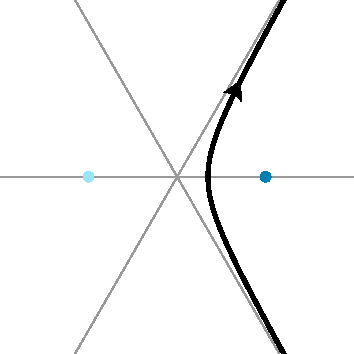
\includegraphics{figures/u_contour_3.pdf}
    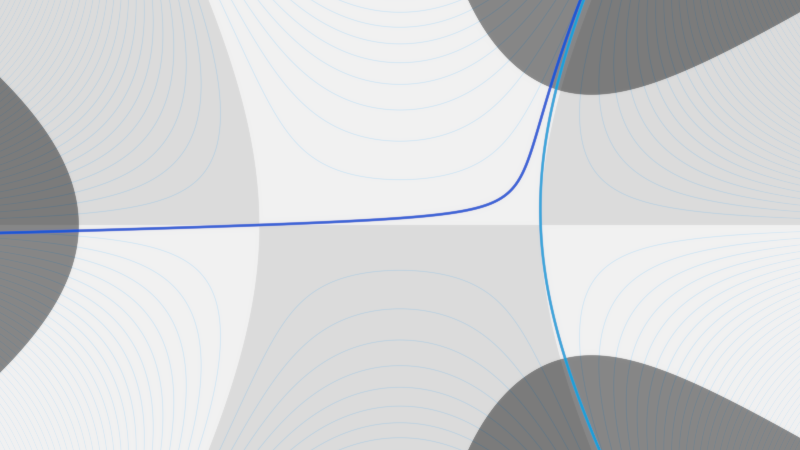
\includegraphics[scale=0.3]{figures/thimble_Airy.png}
    \caption{\small The contour $\Lambda_1$ in the $u$ plane is represented by the light blue path. More generally, the dark blue contour corresponds to the preimage of the ray $+1+e^{i\theta}\infty$ and $\theta=$. While the light blue contour corresponds to the preimage of the ray $-1+e^{i\theta}\infty$. The gray regions correspond to the preimage of $\Re \zeta> \textcolor{orange}{const}$. \textcolor{orange}{[for Aaron: could you please add the correct constant in the description of the figure, and explain what are the different colored regions? Thanks]}}
    \label{fig:path_Airy}
\end{figure}


With the substitution $t = 2uy^{1/2}$, we can rewrite the Airy integral as
\[ \Ai(y) = y^{1/2}\;\frac{1}{\pi i} \int_{y^{-1/2} \Lambda_1} \exp\left[\tfrac{2}{3}y^{3/2} \left(4u^3 - 3u\right)\right]\,du. \]
We have rescaled the contour by a factor of two, but it still approaches $\infty$ in the desired way. Note that $4u^3 - 3u$ is the third Chebyshev polynomial.

By considering other Chebyshev polynomials, we can situate the Airy function within the family of {\em Airy-Lucas functions}, so we’ll go straight to the general case. However, since the Airy function is a classic example in the study of Borel summation and resurgence, it may be useful to see it on its own. For this reason, in Appendix~\ref{airy-appendix} we give a detailed treatment of the Airy function, specializing the general argument of all Airy-Lucas functions.

\subsection{Airy--Lucas}\label{example_AL}
The Airy-Lucas equation is
\begin{equation}\label{eqn:airy-lucas}
\left[\big(\tfrac{\partial}{\partial y}\big)^2 - (m-1) y^{-1} \tfrac{\partial}{\partial y} - y^{n-2}\right] \psi = 0
\end{equation}
with $n \in \{3, 4, 5, \ldots\}$ and $m \in \{1, 2, \ldots, n-1\}$. A few solutions are given by the Airy-Lucas functions~\cite[equation~3.6]{charbonnier22}
\[ \widehat{\Ai}^{(k)}_{n, m-1}(y) = \left\{\begin{array}{ll}1 & j \text{ even} \\ i & j \text{ odd}\end{array}\right\} \frac{y^{m/2}}{\pi} \int_{\Lambda^{(j)}} \exp\left[\tfrac{2}{n} y^{n/2}\,T_n(u)\right]\,U_{m-1}(u)\,du, \]
where $\Lambda_{j}$ is the Lefschetz thimble through $u = \cos\big(\tfrac{j}{n}\pi\big)$ (see Figure \ref{fig:thimble_n_5}).

\begin{figure}[ht]
    \centering
   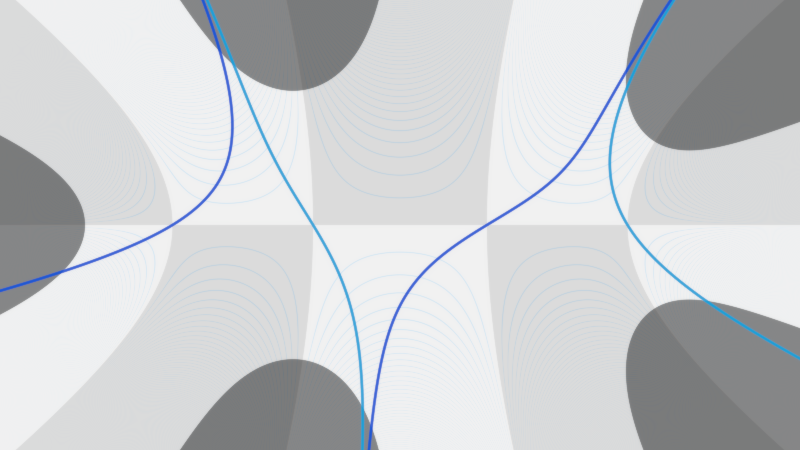
\includegraphics[scale=0.3]{figures/thimble-n5.png}
    \caption{Integration contour $\Lambda_j$ for the Airy--Lucas function with $n=5$. The dark blue contours correspond to the preimage of the ray $1+e^{i\theta}\infty$ and $\theta=???$. While the light blue contours correspond to the preimage of the ray $-1+e^{i\theta}\infty$.}
    \label{fig:thimble_n_5}
\end{figure}


\subsubsection{Rewriting as a modified Bessel $\frac{m}{n}$ equation}
We can distill the most interesting parts of the Airy-Lucas function by writing
\[ \widehat{\Ai}^{(k)}_{n, m-1}(y) = \textcolor{magenta}{\text{const.}}\,y^{{m/2}}\,K\big(\tfrac{2}{n} y^{n/2}\big), \]
where
\begin{equation}\label{integral:mod-bessel-rational-AL}
K_{m/n}(z) = \textcolor{magenta}{\text{const.}} \int_{z^{-{1/n}}\Lambda^{(k)}} \exp\left[z T_n(u)\right]\,U_{m-1}(u)\,du.
\end{equation}
Saying that $\widehat{\Ai}^{(k)}_{n, m-1}$ satisfies the Airy-Lucas equation is equivalent to saying that $K$ satisfies the modified Bessel $\frac{m}{n}$ equation \textcolor{orange}{[Why put the order $m/n$ in the name? Is that standard?]}
\begin{equation}\label{eqn:mod-bessel-AL}
\left[z^2 \big(\tfrac{\partial}{\partial z}\big)^2 + z \tfrac{\partial}{\partial z} - \big[\big(\tfrac{m}{n} \big)^2 + z^2\big]\right] K = 0.
\end{equation}
In fact, as we’ll see in Section~\ref{contour-argument-AL}, $K$ is the modified Bessel function $K_{{m/n}}$.

Let's put equation~\eqref{eqn:mod-bessel-AL} in the form \eqref{eqn:standard ODE}:
\begin{equation}\label{eqn:reg-mod-bessel-AL}
\left[ \big[ \big(\tfrac{\partial}{\partial z}\big)^2 - 1 \big] + z^{-1} \tfrac{\partial}{\partial z} - \big({\tfrac{m}{n}}\big)^2 z^{-2} \right] K = 0.
\end{equation}

\subsubsection{Asymptotic analysis}\label{sec:asympt-AL}

From the general theory of ODE of Poincar\'e rank $1$, we know that the space of trans-series solutions of ~\eqref{eqn:reg-mod-bessel-AL} has a basis of trans-monomials
\[ \{ e^{-\alpha z} z^{-\tau_\alpha}\,\series{W}_\alpha \mid \alpha^2 - 1 = 0 \} \]
where the $\series{W}_\alpha\in\C\llbracket z^{-1} \rrbracket$ are formal power series in $z^{-1}$ and $\tau_\alpha=1/2$. From \cite[Equations 10.40.2 and 10.17.1]{dlmf}, we learn that $K_{m/n}(z) \sim \left(\tfrac{\pi}{2}\right)^{1/2} e^{-z} z^{-1/2}\,\series{W}_1$, with
\begin{equation}\label{bessel-asymp-AL}
\series{W}_1 = 1 - \frac{(\tfrac{1}{2}-\tfrac{m}{n})_1 (\tfrac{1}{2}+\frac{m}{n})_1}{2^1 \cdot 1!}\;z^{-1} + \frac{(\tfrac{1}{2}-\tfrac{m}{n})_2 (\tfrac{1}{2}+\tfrac{m}{n})_2}{2^2 \cdot 2!}\;z^{-2} - \frac{(\tfrac{1}{2}+\tfrac{m}{n})_3 (\tfrac{1}{2}+\tfrac{m}{n})_3}{2^3 \cdot 3!}\;z^{-3} + \ldots
\end{equation}

The holomorphic analysis in Section~\ref{big-idea} will give us holomorphic solutions
\[ \{ e^{-\alpha z} z^{-\tau_\alpha}\,W_\alpha \mid \alpha^2 - 1 = 0 \}, \]
which seem analogous to the trans-monomials above. Borel summation makes the analogy precise. We’ll see in Section~\ref{bessel-regularity-AL} that each $z^{-\tau_\alpha}\,W_\alpha$ is proportional to the Borel sum of $z^{-\tau_\alpha}\,\series{W}_\alpha$. This is evidence of Theorem~4 from \cite{reg-sing-volterra}.
%\subsection{Going to the spatial domain}\label{spatial-AL}
\subsubsection{The big idea}\label{big-idea}
We're going to look for functions $v_\alpha$ whose Laplace transforms $\laplace_{\zeta, \alpha} v_\alpha$ satisfies equation~\eqref{eqn:reg-mod-bessel-AL}. We'll succeed when $\alpha^2 - 1 = 0$, and we'll see that $K_{m/n}$ is a scalar multiple of $\laplace_{\zeta, 1} v_1$.

We can see from Section~\ref{L-int-op} that $\laplace_{\zeta, \alpha} v$ satisfies the differential equation~\eqref{eqn:reg-mod-bessel-AL} if and only if $v$ satisfies the integral equation
\begin{equation}\label{int-eq:spatial-mod-bessel-AL}
\left[ \big[ \zeta^2 - 1 \big] - \fracderiv{-1}{\zeta}{\alpha} \circ \zeta - \big(\tfrac{m}{n}\big)^2 \fracderiv{-2}{\zeta}{\alpha} \right] v = 0.
\end{equation}
It's tempting to differentiate both sides of this equation until we get
\begin{equation}\label{diff-eq:spatial-mod-bessel-AL}
\left[ \big(\tfrac{\partial}{\partial \zeta}\big)^2 \circ \big[ \zeta^2 - 1 \big] - \tfrac{\partial}{\partial \zeta} \circ \zeta - \big(\tfrac{m}{n}\big)^2 \right] v = 0,
\end{equation}
which is easier to solve. Unfortunately, a solution of equation~\eqref{diff-eq:spatial-mod-bessel-AL} won't satisfy equation~\eqref{int-eq:spatial-mod-bessel-AL} in general. However, as we show in Section~\ref{shifting}, a solution of equation~\eqref{diff-eq:spatial-mod-bessel-AL} {\em will} satisfy equation~\eqref{int-eq:spatial-mod-bessel-AL} if it belongs to $\singexpalg{\sigma}(\Omega_j)$, for some $\sigma\in (0,1)$.

This is great news, because equation~\eqref{diff-eq:spatial-mod-bessel-AL} has a regular singularity at each root of $\zeta^2 - 1$, and the Frobenius method often gives a solution of order $\sigma=1/2$ at each regular singular point. We can see the regular singularities by moving the derivatives to the right:
\[ \left[ (\zeta^2 - 1) \big(\tfrac{\partial}{\partial \zeta}\big)^2 + 3\zeta \tfrac{\partial}{\partial \zeta} + \big[ 1 - \big(\tfrac{m}{n}\big)^2 \big] \right] v = 0. \]

In Sections \ref{pos-root-AL}\,--\,\ref{neg-root-AL}, we'll see this approach succeed. For each root $\alpha_j$, we'll find a solution $v_j$ of equation~\eqref{diff-eq:spatial-mod-bessel-AL} which is $\singexpalg{\sigma}(\Omega_j)$, for some $\sigma$, and $\Omega_j$ as in Figure \ref{Fig:domain}. We know the function $\laplace_{\zeta, \alpha} v_\alpha$ will satisfy equation~\eqref{eqn:reg-mod-bessel-AL}, and we can even find its asymptotics from the order $\tau_\alpha$ of $v_\alpha$. We learned in Section~\ref{translation} that
\[ \laplace_{\zeta, \alpha_j} v_j = e^{-\alpha_j z} V_j \]
where $V_j = \laplace_{\zeta_j, 0} v_\alpha$ and $\zeta = \alpha_j + \zeta_j$. We can see from Section~\ref{sec:reg-decay} that $V_j$ is asymptotic to a scalar multiple of $z^{-1 - \tau_j}$ at $z = \infty$, so the further decomposition
\[ \laplace_{\zeta, \alpha_j} v_j = e^{-\alpha_j z} z^{-\tau_j} W_j, \]
makes $W_j$ is asymptotic to a scalar multiple of $z^{-1}$ at $z = \infty$.
%\color{Peru}
%\begin{align*}
%\left[ \big(\tfrac{\partial}{\partial \zeta}\big)^2 \circ (\zeta - 1)(\zeta + 1) - \tfrac{\partial}{\partial \zeta} \circ \zeta - \big(\tfrac{1}{3}\big)^2 \right] v & = 0
%\end{align*}
%\color{Sienna}
%\begin{align*}
%\left[ \big[ 2 + 2(2\zeta) \tfrac{\partial}{\partial \zeta} + (\zeta^2 - 1) \big(\tfrac{\partial}{\partial \zeta}\big)^2 \big] - \big[ 1 + \zeta \tfrac{\partial}{\partial \zeta} \big] - \big(\tfrac{1}{3}\big)^2 \right] v & = 0 \\
%\left[ (\zeta^2 - 1) \big(\tfrac{\partial}{\partial \zeta}\big)^2 + 3\zeta \tfrac{\partial}{\partial \zeta} + \big[ 1 - \big(\tfrac{1}{3}\big)^2 \big] \right] v & = 0 \\
%\left[ (\zeta - 1)(\zeta + 1) \big(\tfrac{\partial}{\partial \zeta}\big)^2 + 3\zeta \tfrac{\partial}{\partial \zeta} + \big[ 1 - \big(\tfrac{1}{3}\big)^2 \big] \right] v & = 0
%\end{align*}
%\color{black}
%%In terms of the coordinate $\zeta_\alpha$ with $\zeta = \alpha + \zeta_\alpha$, this equation is written
%%\begin{equation}\label{eqn:centered-mod-bessel}
%%\[ \left[ \big[ \zeta_\alpha (\zeta_\alpha + 2\alpha) + \alpha^2 - 1 \big] + \fracderiv{-1}{\zeta_\alpha}{0} \circ \big[ \zeta_\alpha + \alpha \big] - \big(\tfrac{1}{3}\big)^2 \fracderiv{-2}{\zeta_\alpha}{0} \right] w = 0. \]
%%\end{equation}
\subsubsection{Focus on $\zeta = 1$}\label{pos-root-AL}
Let's find a solution of equation~\eqref{diff-eq:spatial-mod-bessel-AL} which belongs to $\singexpalg{\sigma}(\Omega_1)$. Define a new coordinate $\zeta_1$ on $\C$ so that $\zeta = 1 + \zeta_1$. In this coordinate, equation~\eqref{diff-eq:spatial-mod-bessel-AL} looks like
\begin{equation}\label{diff-eq:spatial-mod-bessel-pos-AL}
\left[\zeta_1(2 + \zeta_1) \big(\tfrac{\partial}{\partial \zeta_1}\big)^2 + 3(1 + \zeta_1) \tfrac{\partial}{\partial \zeta_1} + \big[1 - \big(\tfrac{m}{n}\big)^2\big]\right] v = 0.
\end{equation}
With another change of coordinate, given by $\zeta_1 = -2\xi_1$, we can rewrite equation~\eqref{diff-eq:spatial-mod-bessel-AL} as the hypergeometric equation
\begin{equation}\label{diff-eq:hypergeom-pos-AL}
\left[\xi_1 (1 - \xi_1) \big(\tfrac{\partial}{\partial \xi_1}\big)^2 + 3(\tfrac{1}{2} - \xi_1) \tfrac{\partial}{\partial \xi_1} - \big[1 - \big(\tfrac{m}{n}\big)^2\big]\right] v = 0.
\end{equation}
Looking through the twenty-four expressions for Kummer's six solutions, we find one \cite[formula~15.10.12]{dlmf} which belongs to $\singexpalg{1/2}$ at $\xi_1 = 0$:
\begin{alignat*}{2}
v_1 &=\;& \hphantom{-i\sqrt{2}}\,\xi_1^{-1/2} & {}_2F_1\big(\tfrac{1}{2}-\tfrac{m}{n}, \tfrac{1}{2}+\tfrac{m}{n}; \tfrac{1}{2}; \xi_1\big) \\
&=\;& -i\sqrt{2}\,\zeta_1^{-1/2} & {}_2F_1\big(\tfrac{1}{2}-\tfrac{m}{n}, \tfrac{1}{2}+\tfrac{m}{n}; \tfrac{1}{2}; -\tfrac{1}{2}\zeta_1\big)
\end{alignat*}
From the argument in Section~\ref{big-idea}, we know that $\laplace_{\zeta, 1} v_1$ satisfies equation~\eqref{eqn:mod-bessel-AL}, and can be written as $e^{-z} V_1$, where $V_1 = \laplace_{\zeta_1, 0} v_1$. Since $v_1$ has order $-1/2$, the decomposition $V_1 = z^{-1/2} W_1$ makes $W_1$ asymptotic to a scalar multiple of $1+O(z^{-1})$ at $z = \infty$.
\subsubsection{Focus on $\zeta = -1$}\label{neg-root-AL}
Let's find a solution of equation~\eqref{diff-eq:spatial-mod-bessel-AL} which belongs to $\singexpalg{\sigma}(\Omega_{-1})$. In the rescaled coordinate from Section~\ref{pos-root-AL}, this is the point $\xi_1 = 1$. Looking again through Kummer's table of solutions, we find another expression \cite[formula~15.10.14]{dlmf} which belongs to $\singexpalg{1/2}$ at $\xi_1 = 1$:
\begin{alignat*}{2}
v_{-1} &=\;& (1-\xi_1)^{-1/2} & {}_2F_1\big(\tfrac{1}{2}-\tfrac{m}{n}, \tfrac{1}{2}+\tfrac{m}{n}; \tfrac{1}{2}; 1-\xi_1\big) \\
&=\;& \sqrt{2}\,\zeta_{-1}^{-1/2} & {}_2F_1\big(\tfrac{1}{2}-\tfrac{m}{n}, \tfrac{1}{2}+\tfrac{m}{n}; \tfrac{1}{2}; \tfrac{1}{2}\zeta_{-1}\big)
\end{alignat*}
where $\zeta_{-1}$ is the coordinate with $\zeta = -1 + \zeta_{-1}$. From the argument in Section~\ref{big-idea}, we know that $\laplace_{\zeta, -1} v_{-1}$ satisfies equation~\eqref{eqn:mod-bessel-AL}, and can be written as $e^z V_{-1}$, where $V_{-1} = \laplace_{\zeta_{-1}, 0} v_{-1}$. Since $v_{-1}$, like our other solution, has order $-1/2$, the same decomposition $V_{-1} = z^{-1/2} W_{-1}$ makes $W_{-1}$ asymptotic to a scalar multiple of $1+O(z^{-1})$ at $z = \infty$.

In this example, $v_1$ and $v_{-1}$ happen to be related by a symmetry: the M\"{o}bius transformation that pulls $\zeta$ back to $-\zeta$. Kummer's solutions typically come from six different hypergeometric equations, which are related by the M\"{o}bius transformations that permute their singularities. In our case, though, exchanging $1$ with $-1$ keeps equation~\eqref{diff-eq:spatial-mod-bessel-AL} the same.
\subsubsection{Abstract argument for Borel regularity}\label{bessel-regularity-AL}
The analysis in Sections~\ref{big-idea}--\ref{neg-root-AL} picks out a frame in the space of analytic solutions of~\eqref{eqn:reg-mod-bessel-AL}. The frame is generated by solutions of the form $\laplace_{\zeta, 1} v_1$ and $\laplace_{\zeta, -1} v_{-1}$, with $v_j\in\singexpalg{1/2}(\Omega_j)$.
\begin{verify}
We get $v_j$ from the existence result in Section~\ref{borel_reg-ODE}, which gives $v_j = \zeta^{\tau-1} + v_j'$ with $\tau \in (0, \infty)$ and $v_j' \in \holoL{\infty, 1-\tau-\epsilon}(\Omega)$ \textcolor{magenta}{[What is this space? Doesn't match notation from {\tt reg-sing-volterra}]} for some $\epsilon \in (0, 1]$. Looking back at the definitions of our weighted $L^\infty$ spaces, we can see that
\begin{align*}
v_j' \in \holoL{\infty, 1-\tau-\epsilon}(\Omega) & \Longrightarrow \zeta_j^{1-\tau-\epsilon}\,v_j' \text{ is bounded near } \zeta_j = 0 \\
& \Longrightarrow \zeta_j^\epsilon\,\zeta_j^{1-\tau-\epsilon}\,v_j' \text{ goes to } 0 \text{ as } \zeta_j \text{ goes to } 0 \\
& \Longrightarrow \zeta_j^{1-\tau}\,v_j' \text{ goes to } 0 \text{ as } \zeta_j \text{ goes to } 0 \\
& \Longrightarrow v_j' / \zeta_j^{\tau-1} \text{ goes to } 0 \text{ as } \zeta_j \text{ goes to } 0 \\
& \Longleftrightarrow v_j' \in o\big(\zeta_j^{\tau-1}\big).
\end{align*}
In this case, $\tau = \tfrac{1}{2}$.
\end{verify}

The Poincar\'{e} algorithm, as we saw in Section~\ref{sec:asympt-AL}, picks out a frame in the space of formal trans-series solutions of equation~\eqref{eqn:reg-mod-bessel-AL}. The frame is generated by trans-monomial solutions of the form $e^{-z} z^{-1/2}\,\tilde{W}_1$ and $e^z z^{-1/2}\,\tilde{W}_{-1}$, with $\tilde{W}_j \in \C\llbracket z^{-1} \rrbracket$. We'll now show that if these solutions are Borel-summable, their Borel sums generate the same frame as $\laplace_{\zeta, 1} v_1$ and $\laplace_{\zeta, -1} v_{-1}$.

The Borel transform maps $e^{-\alpha_j z} z^{-1/2}\,\C\llbracket z^{-1} \rrbracket$ into $\zeta_j^{-1/2}\,\C\llbracket \zeta_j \rrbracket$ (see Section \ref{sec:action_transseries}), and it turns formal trans-monomial solutions of equation~\eqref{eqn:reg-mod-bessel-AL} into formal power series solutions of equation~\eqref{int-eq:spatial-mod-bessel-AL}. Summation sends convergent power series in $\zeta_j^{-1/2}\,\C\llbracket \zeta_j \rrbracket$ into $\zeta_j^{-1/2}+ o\big(\zeta_j^{-1/2}\big)$ \textcolor{orange}{[since the argument above is one-way, isn't this weaker than being in $\singexpalg{1/2}$?]}, and it turns convergent power series that satisfy a given fractional integral equation into holomorphic functions that satisfy the same equation \cite[Lemma 2]{reg-sing-volterra}. Thus, if $e^{-z} z^{-1/2}\,\tilde{W}_1$ and $e^z z^{-1/2}\,\tilde{W}_{-1}$ are $1$-Gevrey, their Borel transforms sum to solutions of equation~\eqref{int-eq:spatial-mod-bessel-AL}, which lie in $\singexpalg{1/2}$ \textcolor{orange}{[needs domain]} for $\alpha = 1$ and $\alpha = -1$, respectively.

When $\alpha$ is $1$ or $-1$, equation~\eqref{int-eq:spatial-mod-bessel-AL} becomes the kind of singular integral equation discussed in Section~\ref{borel_reg-ODE}. It therefore has exactly one solution in $\singexpalg{1/2}$ \textcolor{orange}{[needs domain]}, up to scaling. That means $\borel\big[ e^{-\alpha_j z} z^{-1/2}\,\tilde{W}_j \big]$ must sum to a scalar multiple of $v_j$. Thus, if $e^{-\alpha_j z} z^{-1/2}\,\tilde{W}_j$ is Borel-summable, its Borel sum is a scalar multiple of $\laplace_{\zeta, \alpha_j} v_j$.

\subsubsection{Confirmation of Borel regularity}\label{confirmation-borel-regularity}
We can confirm the conclusion of Section~\ref{bessel-regularity-AL} using our explicit expressions for the formal power series $\tilde{W}_\alpha$ and the functions $v_\alpha$. We found in Section~\ref{sec:asympt-AL} that
\begin{align*}
\tilde{W}_1 & = \sum_{k = 0}^{\infty} \frac{\left(\tfrac{1}{2}-\tfrac{m}{n}\right)_k \left(\tfrac{1}{2}+\tfrac{m}{n}\right)_k}{k!} \left(-\frac{1}{2}\right)^k z^{-k} \\
\tilde{W}_{-1} & = \sum_{k = 0}^{\infty} \frac{\left(\tfrac{1}{2}-\tfrac{m}{n}\right)_k \left(\tfrac{1}{2}+\tfrac{m}{n}\right)_k}{k!} \left(\frac{1}{2}\right)^k z^{-k}.
\end{align*}
Computing
\begin{align*}
\borel_\zeta \big[ e^{-z} z^{-1/2}\,\tilde{W}_1 \big] & = \borel_\zeta \left[ e^{-z} \sum_{k = 0}^{\infty} \frac{\left(\tfrac{1}{2}-\tfrac{m}{n}\right)_k \left(\tfrac{1}{2}+\tfrac{m}{n}\right)_k}{k!} \left(-\frac{1}{2}\right)^k z^{-k-\frac{1}{2}} \right] \\
& = \sum_{k = 0}^{\infty} \frac{\left(\tfrac{1}{2}-\tfrac{m}{n}\right)_k \left(\tfrac{1}{2}+\tfrac{m}{n}\right)_k}{k!} \left(-\frac{1}{2}\right)^k \frac{\zeta_1^{k-\frac{1}{2}}}{\Gamma\big(k+\frac{1}{2}\big)} \\
& = \sum_{k = 0}^{\infty} \frac{\left(\tfrac{1}{2}-\tfrac{m}{n}\right)_k \left(\tfrac{1}{2}+\tfrac{m}{n}\right)_k}{k!} \left(-\frac{1}{2}\right)^k \frac{\zeta_1^{k-\frac{1}{2}}}{\Gamma\big(\frac{1}{2}\big) \left(\frac{1}{2}\right)_k} \\
& = \frac{\zeta_1^{-\frac{1}{2}}}{\Gamma\big(\frac{1}{2}\big)} \sum_{k = 0}^{\infty} \frac{\left(\tfrac{1}{2}-\tfrac{m}{n}\right)_k \left(\tfrac{1}{2}+\tfrac{m}{n}\right)_k}{\left(\frac{1}{2}\right)_k} \left(-\frac{1}{2}\right)^k \frac{\zeta_1^k}{k!},
\end{align*}
we see that $\borel\big[ e^{-z} z^{-1/2}\,\tilde{W}_1 \big]$ sums to
\[ \tfrac{1}{\Gamma(1/2)}\,\zeta_1^{-1/2}\,{}_2F_1\big(\tfrac{1}{2}-\tfrac{m}{n}, \tfrac{1}{2}+\tfrac{m}{n}; \tfrac{1}{2}; -\tfrac{1}{2}\zeta_1\big). \]
Looking back at Section~\ref{pos-root-AL}, we recognize this as a scalar multiple of $v_1$. In fact, with the thimble projection reasoning, there is no ambiguity in the choice of the multiplicative constant. 


Through a similar calculation, we see that $\borel\big[ e^z z^{-1/2}\,\tilde{W}_{-1} \big]$ sums to
\[ \tfrac{1}{\Gamma(1/2)}\,\zeta_{-1}^{-1/2}\,{}_2F_1\big(\tfrac{1}{2}-\tfrac{m}{n}, \tfrac{1}{2}+\tfrac{m}{n}; \tfrac{1}{2}; \tfrac{1}{2}\zeta_{-1}\big). \]
Looking back at Section~\ref{neg-root-AL}, we recognize this as a scalar multiple of $v_{-1}$.



\subsubsection{Thimble projection reasoning for Airy-Lucas functions}\label{contour-argument-AL}
\textcolor{orange}{[\textbf{New phrasing for rewrite:} The critical point splits the thimble $\Lambda$ into two pieces: the {\em incoming} branch, where the orientation of the thimble runs toward the critical point, and the {\em outgoing} branch, where the orientation points away.]}
We follow the reasoning of the proof of Theorem~\ref{thm:maxim}.
We can recast integral~\eqref{integral:mod-bessel-rational-AL} into the $\zeta$ plane by setting $\textcolor{magenta}{-\zeta} = T_n(u)$, which implies that $-d\zeta = n U_{n-1}(u)\,du$. Projecting $z^{-1/n} \Lambda^{(k)}$ to a contour $\gamma_z$ in the $\zeta$ plane and choosing the branch of $u$ that lifts $\gamma_z$ back to $z^{-1/n} \Lambda^{(k)}$, we get \textcolor{magenta}{[sign flipped]} 

\begin{align*}%%\label{integral:mod-bessel-rational-zeta}
K_{m/n}(z) & = \frac{n}{2 \sinh\big(\tfrac{m}{n}\,i\pi\big)} \int_{z^{-\textcolor{DarkCyan}{1/n}}\Lambda^{(k)}} \exp\left[z T_n(u)\right]\,U_{m-1}(u)\,du \\
& = -\frac{1}{2  \sinh\big(\tfrac{m}{n}\,i\pi\big)} \int_{\gamma_z} e^{-z\zeta}\,\frac{U_{m-1}(u)}{U_{n-1}(u)}\,d\zeta %\\
%& = -\frac{1}{2\,\tfrac{n}{m} \sinh\big(\tfrac{m}{n}\,i\pi\big)} \int_{\gamma_z} e^{-z\zeta}\,F(1 - \tfrac{m}{n}, 1 + \tfrac{m}{n}, \tfrac{3}{2}, \tfrac{1}{2} \pm \tfrac{1}{2}\zeta)\,d\zeta.
\end{align*}


For $z \in (0, \infty)$, the contour $\gamma_z$ runs \textcolor{magenta}{counterclockwise} around $[1, \infty)$, as shown below\textcolor{DarkCyan}{, so we have to choose the negative sign above (?)}. Let's assume $z \in (0, \infty)$ for the rest of the section. \textcolor{magenta}{[Our conclusions should probably hold whenever $\operatorname{Re}(z) > 0$.]}


\begin{center}
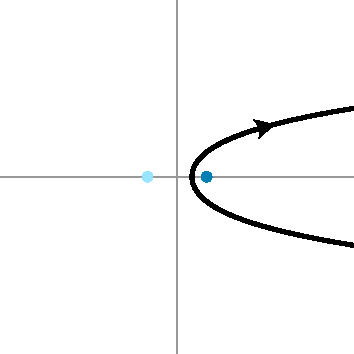
\includegraphics{figures/zeta_contour_3.pdf} \\[1em]
{\small The contour $\gamma_1$ \textcolor{magenta}{[reversed]} in the $\zeta$ plane, slightly off from the critical value $\zeta=1$.}
\end{center}

Now we observe, that by properties of Chebyshev polynomials the integrand can be written as an explicit function of $\zeta$: 

\begin{align*}
    \frac{U_{m-1}(\cos(\phi))}{U_{n-1}(\cos(\phi))}&=\frac{\sin(m\phi)}{\sin(\phi)}\frac{\sin(\phi)}{\sin(n \phi)}\\
    &=\frac{\sin(m\phi)}{\sin(n \phi)}\\
    &=\frac{m}{n}\,\, {}_2F_1\left(\frac{1}{2}-\frac{m}{2n},\frac{1}{2}+\frac{m}{2n};\frac{3}{2};\sin^2(n \phi)\right)\\
    &=\frac{m}{n}\,\, {}_2F_1\left(\frac{1}{2}-\frac{m}{2n},\frac{1}{2}+\frac{m}{2n};\frac{3}{2};1-\zeta^2\right) 
\end{align*}
where in the last step we use $-\zeta=T_n(u)=T_n(\cos\phi)=\cos(n\phi)$. Applying identity 15.8.4, 15.8.27 and 15.8.28 from \cite{dlmf}, 

\begin{align*}
    &{}_2F_1\left(\frac{1}{2}-\frac{m}{2n},\frac{1}{2}+\frac{m}{2n};\frac{3}{2};1-\zeta^2\right)=\\
    &\qquad = \frac{\pi}{\Gamma\left(1-\frac{m}{2n}\right)\Gamma\left(1+\frac{m}{2n}\right)} \,\,\, {}_2F_1\left(\frac{1}{2}-\frac{m}{2n},\frac{1}{2}+\frac{m}{2n};\frac{1}{2};\zeta^2\right)+\\
    &\qquad \qquad\qquad - \frac{\pi \zeta}{\Gamma\left(\frac{1}{2}-\frac{m}{2n}\right)\Gamma\left(\frac{1}{2}+\frac{m}{2n}\right)} \,\,\, {}_2F_1\left(1-\frac{m}{2n},1+\frac{m}{2n};\frac{3}{2};\zeta^2\right)\\
    &\qquad ={}_2F_1\left(1-\frac{m}{n},1+\frac{m}{n};\frac{3}{2};\frac{1}{2}-\frac{\zeta}{2}\right)+{}_2F_1\left(1-\frac{m}{n},1+\frac{m}{n};\frac{3}{2};\frac{1}{2}+\frac{\zeta}{2}\right)+\\
    &\qquad\qquad +\frac{1}{2} {}_2F_1\left(1-\frac{m}{n},1+\frac{m}{n};\frac{3}{2};\frac{1}{2}-\frac{\zeta}{2}\right)-\frac{1}{2}{}_2F_1\left(1-\frac{m}{n},1+\frac{m}{n};\frac{3}{2};\frac{1}{2}+\frac{\zeta}{2}\right)\\
    &\qquad =\frac{3}{2} {}_2F_1\left(1-\frac{m}{n},1+\frac{m}{n};\frac{3}{2};\frac{1}{2}-\frac{\zeta}{2}\right)+\frac{1}{2}{}_2F_1\left(1-\frac{m}{n},1+\frac{m}{n};\frac{3}{2};\frac{1}{2}+\frac{\zeta}{2}\right)
\end{align*}
In addition, recall that ${}_2F_1\left(1-\frac{m}{n},1+\frac{m}{n};\frac{3}{2};\frac{1}{2}-\frac{\zeta}{2}\right)$ has a branch cut singularity at $\zeta=-1$ while ${}_2F_1\left(1-\frac{m}{n},1+\frac{m}{n};\frac{3}{2};\frac{1}{2}+\frac{\zeta}{2}\right)$ has a branch cut at $\zeta=1$; hence 

\begin{align*}
    K_{m/n}(z)&=-\frac{m}{4 n\sinh(\tfrac{m}{n}i\pi)}\int_{\gamma_z}e^{-z\zeta} {}_2F_1\left(1-\frac{m}{n},1+\frac{m}{n};\frac{3}{2};\frac{1}{2}+\frac{\zeta}{2}\right) d\zeta\\
    &=-\frac{1}{2}\int_{1}^{+\infty}e^{-z\zeta} \left(-\frac{1}{2}+\frac{\zeta}{2}\right)^{-1/2} {}_2F_1\left(\frac{1}{2}-\frac{m}{n},\frac{1}{2}+\frac{m}{n};\frac{1}{2};\frac{1}{2}-\frac{\zeta}{2}\right) d\zeta
\end{align*}

where in the second step we use the analytic continuation of the hypergeometric function \cite[Equation 15.2.3]{dlmf}. 

Finally, comparing this expression for $K_{m/n}$ with the expression for $v_1$ computed in Section \ref{pos-root} we notice that 
\begin{align*}
    K_{m/n}(z)=\frac{i}{2}\laplace_{\zeta,1}v_1 .
\end{align*}

\subsubsection{A flavor of resurgence: the Stokes phenomena in the position domain}\label{resurgence-AL}

In the previous sections, we have seen how to compute the Borel transform of a formal frame of solutions of the modified Bessel equation with parameter $m/n$ (Section \ref{confirmation-borel-regularity}) or equivalently of the asymptotic expansion of thimble integrals $K_{m/n}$ (Section \ref{contour-argument-AL}). In both cases we find 
\begin{align*}
    v_1(\zeta)= i \left(-\frac{1}{2}+\frac{\zeta}{2}\right)^{-1/2} {}_2F_1\left(\frac{1}{2}-\frac{m}{n},\frac{1}{2}+\frac{m}{n};\frac{1}{2};\frac{1}{2}-\frac{\zeta}{2}\right)
\end{align*}
which has a fractional power singularity at $\zeta=1$. In addition, the hypergeometric function ${}_2F_1\left(\frac{1}{2}-\frac{m}{n},\frac{1}{2}+\frac{m}{n};\frac{1}{2};\frac{1}{2}-\frac{\zeta}{2}\right)$ is convergent at $\zeta=1$ therefore $v_1$ has the typical form of a \textit{singularity} in the formalism of \'Ecalle's resurgent functions. More precisely, we can consider ${}_2F_1\left(\frac{1}{2}-\frac{m}{n},\frac{1}{2}+\frac{m}{n};\frac{1}{2};\frac{1}{2}-\frac{\zeta}{2}\right)$ as a new holomorphic function (analytic continuation of a new germ at the origin), which has a branch cut singularity at $\zeta=-1$. Using equation \cite[15.2.3]{dlmf}, we can compute the analytic continuation of this germ at $\zeta=-1$: 
\begin{align*}
&{}_2F_1\left(\frac{1}{2}-\frac{m}{n},\frac{1}{2}+\frac{m}{n};\frac{1}{2};-\frac{\zeta_1}{2}+i\varepsilon\right)-{}_2F_1\left(\frac{1}{2}-\frac{m}{n},\frac{1}{2}+\frac{m}{n};\frac{1}{2};-\frac{\zeta_1}{2}-i\varepsilon\right)=\\
&=\frac{2\pi i}{\Gamma\big(\tfrac{1}{2}-\tfrac{m}{n}\big)\Gamma\big(\tfrac{1}{2}+\tfrac{m}{n}\big)} \left(-\frac{\zeta_{-1}}{2}\right)^{-1/2} {}_2F_1\left(\frac{m}{n},-\frac{m}{n};\frac{1}{2};\frac{\zeta_{-1}}{2}\right) \\
&=2 i\cos(\pi m/n) \left(-\frac{\zeta_{-1}}{2}\right)^{-1/2} {}_2F_1\left(\frac{m}{n},-\frac{m}{n};\frac{1}{2};\frac{\zeta_{-1}}{2}\right) \\
&=2\cos(\pi m/n) \left(\frac{\zeta_{-1}}{2}\right)^{-1/2} {}_2F_1\left(\frac{m}{n},-\frac{m}{n};\frac{1}{2};\frac{\zeta_{-1}}{2}\right) \\
&=2\cos(\pi m/n)\, \left(\frac{\zeta_{-1}}{2}\right)^{-1/2} \left(-\frac{\zeta_{1}}{2}\right)^{1/2}\, {}_2F_1\left(\frac{1}{2}-\frac{m}{n},\frac{1}{2}+\frac{m}{n};\frac{1}{2};\frac{\zeta_{-1}}{2}\right)
\end{align*}
Hence, we deduce  
\begin{equation}\label{resurgent-relation-1}
    v_1(\zeta+1+i\varepsilon)-v_1(\zeta+1+i\varepsilon)=2i \cos(\pi m/n)  v_{-1}(\zeta)
\end{equation}
namely, that the germ of the singularity at $\zeta=1$ knows about the germ of the singularity at $\zeta=-1$. This is an instance of \textit{resurgent functions}, introduced by \'Ecalle in \cite{EcalleI,EcalleII,EcalleIII}\footnote{If the reader is interested in resurgence, it may be useful to look at the following review \cite{diverg-resurg-i,Dorigoni,aniceto2019primer}.}. Although we’ll not discuss more about resurgence, we would like to point out that among the great advantages of resurgence (for instance compared to Borel summability) there are the \textit{formalism of singularities} and the \textit{Alien calculus} which allow to understand the Stokes phenomena working in the position domain. The same phenomena were described by Berry and Howls \cite{Berry_Howls} who noticed that divergent asymptotic expansions of thimble integrals encode the contribution of other critical values. 

We can repeat the same reasoning with $v_{-1}$:
\begin{align*}
    v_{-1}(\zeta)=  \left(\frac{1}{2}+\frac{\zeta}{2}\right)^{-1/2} {}_2F_1\left(\frac{1}{2}-\frac{m}{n},\frac{1}{2}+\frac{m}{n};\frac{1}{2};\frac{1}{2}+\frac{\zeta}{2}\right)
\end{align*}
and ${}_2F_1\left(\frac{1}{2}-\frac{m}{n},\frac{1}{2}+\frac{m}{n};\frac{1}{2};\frac{1}{2}+\frac{\zeta}{2}\right)$ is singular at $\zeta=1$. Hence
\begin{align*}
&{}_2F_1\left(\frac{1}{2}-\frac{m}{n},\frac{1}{2}+\frac{m}{n};\frac{1}{2};\frac{\zeta_{-1}}{2}+i\varepsilon\right)-{}_2F_1\left(\frac{1}{2}-\frac{m}{n},\frac{1}{2}+\frac{m}{n};\frac{1}{2};\frac{\zeta_{-1}}{2}-i\varepsilon\right)=\\
&=\frac{2\pi i}{\Gamma\big(\tfrac{1}{2}-\tfrac{m}{n}\big)\Gamma\big(\tfrac{1}{2}+\tfrac{m}{n}\big)} \left(\frac{\zeta_{1}}{2}\right)^{-1/2} {}_2F_1\left(\frac{m}{n},-\frac{m}{n};\frac{1}{2};-\frac{\zeta_{1}}{2}\right) \\
&=2 i\cos(\pi m/n) \left(\frac{\zeta_{1}}{2}\right)^{-1/2} {}_2F_1\left(\frac{m}{n},-\frac{m}{n};\frac{1}{2};-\frac{\zeta_{1}}{2}\right) \\
&=2i \cos(\pi m/n)\, \left(\frac{\zeta_{1}}{2}\right)^{-1/2} \left(\frac{\zeta_{-1}}{2}\right)^{1/2}\, {}_2F_1\left(\frac{1}{2}-\frac{m}{n},\frac{1}{2}+\frac{m}{n};\frac{1}{2};-\frac{\zeta_{1}}{2}\right)
\end{align*}
and the analogue of \eqref{resurgent-relation-1} is 
\begin{equation}\label{resurgent-realtion-2}
    v_{-1}(\zeta-1+i\varepsilon)-v_{-1}(\zeta-1-i\varepsilon)= -2i\cos(\pi m/n) v_1(\zeta).
\end{equation}
Equations \eqref{resurgent-relation-1} and \eqref{resurgent-realtion-2} are a manifestation of the Stokes phenomena, already in the position domain. Indeed, when we start varying the contour of integration for the Laplace transform, we know that $\laplace_{\zeta,1}^\pi$ and $\laplace_{\zeta,-1}^0$ are not well defined because the contour hits the other singularity (respectively at $\zeta=-1$ and $\zeta=1$). The Stokes phenomenon consists of comparing the Laplace transform below and above the critical direction and it quantifies the jump as a constant (the so-called Stokes constant) times another function. In our example:
\begin{align*}
    \laplace_{\zeta,1}^{\pi+\varepsilon} v_1-\laplace_{\zeta,1}^{\pi-\varepsilon} v_1 & = 2 i \cos(\pi m/n) \, e^{-z}\, \laplace_{\zeta,-1}^{\pi} v_{-1} \\
    \laplace_{\zeta,-1}^{\varepsilon} v_{-1}-\laplace_{\zeta,-1}^{-\varepsilon} v_{-1} & = - 2 i \cos(\pi m/n)  \, e^z \, \laplace_{\zeta,1} v_{1} 
\end{align*}
thus the Stokes constants are respectively $\pm 2i \cos(\pi m/n)$\footnote{If we think of the Laplace transforms of $v_1$ and $v_{-1}$ as a frame of solutions for the Airy--Lucas differential equation, the equations above define the so-called Stokes matrices for the ODE.}. 

It may be surprising that the Stokes constants depend on $\cos(\pi m/n)$, as the Stokes constants are the intersection number of \textit{dual pairs of thimbles}, according to Picard--Lefschetz formula (in particular, they are integers in a suitable normalization), see \cite[Section 5]{pham} and \cite[Chapter ??]{Arnold}. However, in the Airy--Lucas example, $f$ is not Morse (unless $n=3$), hence we have to interpret the $\cos(\pi m/n)$ as a consequence of the ambiguity on the lift of a path in the position domain. \textcolor{orange}{ I think we should argue we have the action of the permutation which leaves the base unchanged but gives a } 




%\textcolor{DarkCyan}{where the sign must be chosen so that $\pm\zeta$ stays in the left half-plane over the whole integration path (?)}.
%For $z \in (0, \infty)$, the contour $\gamma_z$ runs \textcolor{magenta}{counterclockwise} around $[1, \infty)$, as shown below\textcolor{DarkCyan}{, so we have to choose the negative sign above (?)}. Let's assume $z \in (0, \infty)$ for the rest of the section. \textcolor{magenta}{[Our conclusions should probably hold whenever $\operatorname{Re}(z) > 0$.]}


%The integrand is non-meromorphic at $\zeta = 1$. Along the branch cut $\zeta \in [1, \infty)$, its above-minus-below difference is
%\begin{align*}
%& -(2\pi i)\tfrac{n}{2\pi m} \sin(\tfrac{m}{n} \pi)\,(\pm\tfrac{1}{2}\zeta - \tfrac{1}{2})^{-1/2} {}_2F_1(\tfrac{1}{2} - \tfrac{m}{n}, \tfrac{1}{2} + \tfrac{m}{n}, \tfrac{1}{2}, \tfrac{1}{2} \mp \tfrac{1}{2}\zeta) \\
%= & -\tfrac{n}{m} \sinh(\tfrac{m}{n}\,i\pi)\,(\pm\tfrac{1}{2}\zeta - \tfrac{1}{2})^{-1/2} {}_2F_1(\tfrac{1}{2} - \tfrac{m}{n}, \tfrac{1}{2} + \tfrac{m}{n}, \tfrac{1}{2}, \tfrac{1}{2} \mp \tfrac{1}{2}\zeta),
%\end{align*}
%as given\footnote{Note that $\Gamma(\tfrac{3}{2}) \Gamma(\tfrac{1}{2})^{-1} = \tfrac{1}{2}$ and $\big[\Gamma(1 - \tfrac{m}{n})\Gamma(1 + \tfrac{m}{n})\big]^{-1} = \big[\Gamma(1 - \tfrac{m}{n})\,\tfrac{m}{n}\Gamma(\tfrac{m}{n})\big]^{-1} = \tfrac{n}{m\pi} \sin(\tfrac{m}{n} \pi)$.} by equation~15.2.3 from \cite{dlmf}. Hence, $K_{m/n}$ turns out to be the Laplace transform along $(1, \infty)$ of
%\[ \tfrac{1}{2}\,(-\tfrac{1}{2}\zeta - \tfrac{1}{2})^{-1/2} F(\tfrac{1}{2} - \tfrac{m}{n}, \tfrac{1}{2} + \tfrac{m}{n}, \tfrac{1}{2}, \tfrac{1}{2} + \tfrac{1}{2}\zeta). \]
%\color{DarkCyan}
%Guessing the branch of the square root for consistency with the numerically checked result in Section~\ref{contour-argument}, we get
%\[ \tfrac{i}{2}\,(\tfrac{1}{2} + \tfrac{1}{2}\zeta)^{-1/2} F(\tfrac{1}{2} - \tfrac{m}{n}, \tfrac{1}{2} + \tfrac{m}{n}, \tfrac{1}{2}, \tfrac{1}{2} + \tfrac{1}{2}\zeta). \]
%In other words, $K_{m/n} = \tfrac{i}{2} \laplace_{\zeta, -1} v_{-1}$ with
%\[ v_{-1} = \sqrt{2}\,\zeta_{-1}^{-1/2} F(\tfrac{1}{2} - \tfrac{m}{n}, \tfrac{1}{2} + \tfrac{m}{n}, \tfrac{1}{2}, \tfrac{1}{2}\zeta_{-1}), \]
%where $\zeta = -1 + \zeta_{-1}$.
%\color{black}


\subsection{Modified Bessel}\label{sec:mod-bessel-lift}

The modified Bessel equation is a generalization of equation~\eqref{eqn:mod-bessel-AL} where $\frac{m}{n}$ is replaced by a complex parameter $\mu$
\begin{equation}\label{eqn:mod-bessel}
\left[z^2 \big(\tfrac{\partial}{\partial z}\big)^2 + z \tfrac{\partial}{\partial z} - \big[\mu^2 + z^2\big]\right] \varphi = 0
\end{equation}
On the one hand, this new condition does not really affect the argument we present in Section~\ref{bessel-regularity-AL}, so we briefly state the main results: 
\begin{itemize}
 \item \textbf{Asymptotic analysis}: equation~\eqref{eqn:mod-bessel} admits a basis of formal solutions \[\series{I}_{\mu,1}(z)=e^{-z} z^{-1/2} \tilde{W}_{\mu, 1} \quad \text{ and } \quad \series{I}_{\mu,-1}(z)=e^z z^{-1/2} \series{W}_{\mu, -1}\] with 
 \begin{align*}
 \tilde{W}_{\mu,1} &= 1- \frac{\big(\tfrac{1}{2}-\mu\big)\big(\frac{1}{2}+\mu\big)}{2 \cdot 1!} z^{-1} + \frac{\big(\tfrac{1}{2}-\mu\big)_2\big(\frac{1}{2}+\mu\big)_2}{2^2 \cdot 2!} z^{-2} - \frac{\big(\tfrac{1}{2}-\mu\big)_3\big(\frac{1}{2}+\mu\big)_3}{2^3 \cdot 3!} z^{-3}+...\\
 \series{W}_{\mu,-1} &= 1+\frac{\big(\tfrac{1}{2}-\mu\big)\big(\frac{1}{2}+\mu\big)}{2 \cdot 1!} z^{-1} + \frac{\big(\tfrac{1}{2}-\mu\big)_2\big(\frac{1}{2}+\mu\big)_2}{2^2 \cdot 2!} z^{-2}+ \frac{\big(\tfrac{1}{2}-\mu\big)_3\big(\frac{1}{2}+\mu\big)_3}{2^3 \cdot 3!} z^{-3} + ...
\end{align*}   
 \item  \textbf{Frame of analytic solutions}: there exist two functions $v_{\mu, 1}, v_{\mu, -1}$ such that $\laplace_{\alpha}v_{\mu, \alpha}$ satisfies equation~\eqref{eqn:mod-bessel} and they are explicitly 
\begin{align*}
v_{\mu, 1}&=-i\sqrt{2}\,\zeta_{1}^{-1/2}  {}_2F_1\big(\tfrac{1}{2}-\mu, \tfrac{1}{2}+\mu; \tfrac{1}{2}; -\tfrac{1}{2}\zeta_{1}\big)\\
v_{\mu, -1}&=\sqrt{2}\,\zeta_{-1}^{-1/2}  {}_2F_1\big(\tfrac{1}{2}-\mu, \tfrac{1}{2}+\mu; \tfrac{1}{2}; \tfrac{1}{2}\zeta_{-1}\big)
\end{align*}
\item \textbf{Borel regularity} We can compare the Borel transform of the formal solutions $\series{W}_{\mu,\pm1}$ with the analytic solutions $v_{\mu,\pm 1}$. They agree (up to the choice of a constant), hence we have another example where Borel regularity can be explicitly verified. 
\end{itemize}
On the other hand, the thimble projection reasoning we describe in Section~\ref{contour-argument-AL} has to be generalized, as we’ll discuss in the following Section~\ref{countable-cover}. 

\subsubsection{Lifting to a countable cover}\label{countable-cover}
Formula~\eqref{integral:mod-bessel-rational-AL} expresses the modified Bessel function $K_{m/n}$ as an exponential integral on a finite cover of $\C$. Lifting to a countable cover reveals this formula as a special case of a general integral formula for modified Bessel functions.

Setting $u = \cosh(t/n)$ and recalling that
\begin{align*}
\cosh(n\tau) & = T_n(\cosh(\tau)) \\
\sinh(m\tau) & = U_{m-1}(\cosh(\tau)) \sinh(\tau),
\end{align*}
we can rewrite formula~\eqref{integral:mod-bessel-rational-AL} as \textcolor{magenta}{[switching to the conventional sign for the projection map, so $\Lambda^{(3)}$ now comes from $\infty$ at $-60^\circ$ and goes to $\infty$ at $60^\circ$]}
\begin{align}
\notag K_{m/n}(z) & = \frac{n}{2 \sinh\big(\tfrac{m}{n}\,i\pi\big)} \int_{z^{-\textcolor{DarkCyan}{1/n}}\Lambda^{(k)}} \exp\left[z T_n(u)\right]\,U_{m-1}(u)\,du \\
\notag & = \frac{n}{2 \sinh\big(\tfrac{m}{n}\,i\pi\big)} \int_{\textcolor{magenta}{\Lambda_j}} \exp\left[z \cosh(t)\right]\,U_{m-1}(\cosh(t/n))\,\sinh(t/n)\,d(t/n) \\
\label{integral:mod-bessel-lifted} & = \frac{1}{2 \sinh\big(\tfrac{m}{n}\,i\pi\big)} \int_{\textcolor{magenta}{\Lambda_j}} \exp\left[z \cosh(t)\right]\,\sinh\big(\tfrac{m}{n}\,t\big)\,dt.
\end{align}
where $\Lambda_j$ is the path coming from infinity along $-i\pi+(2\pi i) j+(-\infty,0]$ and going to infinity along $i \pi+(2\pi i) j+[0,+\infty)$, as represented in Figure \ref{fig:bessel_unrolled}. In fact, since $\cosh(t)$ is periodic, the integral has the same value for every choice of $\Lambda_j$ with $j\in\Z$.  
\begin{figure}[ht]
    \centering
    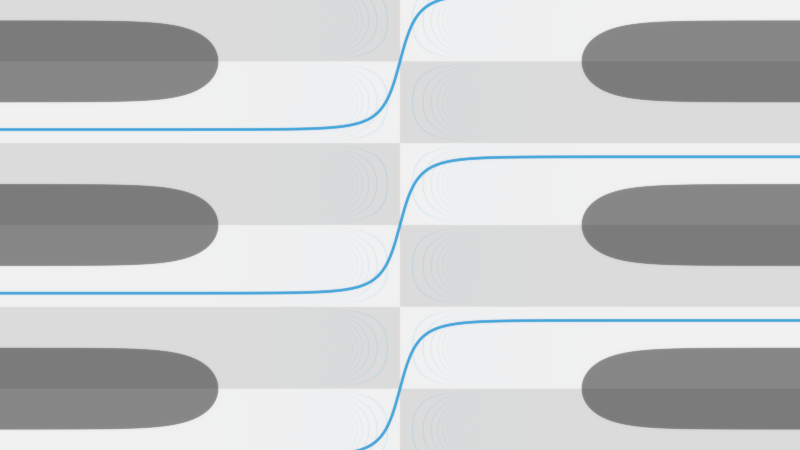
\includegraphics[scale=0.3]{figures/Bessel0_unrolled_lightblue.png}
    \caption{The paths $\Lambda_j$.}
    \label{fig:bessel_unrolled}
\end{figure}

For any $\mu \in \C \smallsetminus \Z$, we have a thimble integral representation of $K_{\mu}$ given by formulas 10.32(ii) and 10.27.4 of \cite{dlmf}\textcolor{DarkCyan}{[Cite Watson too?]}
\begin{equation}\label{int:mod-bessel-gen}
 K_\mu(z) = \frac{1}{2 \sinh(\mu\,i\pi)} \int_{\Lambda_0} \exp\left[z \cosh(t)\right]\,\sinh(\mu t)\,dt,
\end{equation}
\begin{verify}
   % \begin{align*}
   %    \notag K_\mu(z) & = \frac{\pi}{\sin(\mu \pi)} \cdot \frac{1}{2}\big[ I_{-\mu}(z) - I_\mu(z) \big] \\
%\notag & = \frac{1}{2i \sin(\mu \pi)} \int_{\Lambda'} \exp\left[z \cosh(t)\right]\,\frac{1}{2}\left[e^{\mu t} - e^{-\mu t}\right]\,dt 
 %   \end{align*}
  %  where $\Lambda'$ is a path that comes from $\infty$ along $-i \pi + (0, \infty)$ and goes to $\infty$ along $i \pi + (0, \infty)$ 
  Following Watson \textit{A treatment of Bessel function}, 1944, pp. 181 (it's the reference in \cite{dlmf})
    \begin{align*}
        2\pi i \, I_\mu(z) &= \int_{+\infty}^0 e^{z\cosh(-\pi i+a)-\mu(-i\pi +a)} da + \int_{0}^{+\infty} e^{z\cosh(\pi i+a)-\mu(i\pi +a)} da +\int_{-\pi}^{\pi} e^{z\cosh(ib)-\mu i b} db\\
        &=-\int_{-\infty}^0 e^{z\cosh(-\pi i-a)+\mu(i \pi +a)} da + \int_{0}^{+\infty} e^{z\cosh(\pi i+a)-\mu(i \pi  +a)} da +\int_{0}^{\pi} e^{z\cosh(ib)}\cosh(i\mu b) db\\
        &=-\int_{-\infty}^0 e^{z\cosh(\pi i+a)+\mu(i\pi +a)} da + \int_{0}^{+\infty} e^{z\cosh(\pi i+a)-\mu(i\pi +a)} da +\int_{0}^{\pi} e^{z\cosh(ib)}\cosh(i\mu b) db
    \end{align*}
    hence 
    \begin{align*}
   4 i \sin(\mu \pi) K_\mu(z) & = 2\pi i \big[ I_{-\mu}(z) - I_\mu(z) \big]\\
     &= \int_{-\infty}^0 e^{z\cosh(\pi i+a)}\left[-e^{-\mu(i\pi +a)}+e^{\mu(i\pi +a)}\right] da + \int_{0}^{+\infty} e^{z\cosh(\pi i+a)}\left[e^{\mu(i\pi +a)}-e^{-\mu(i\pi +a)}\right] da \\
        &=2\int_{-\infty}^0 e^{z\cosh(\pi i+a)} \sinh(a+i\pi) da + 2\int_{0}^{+\infty} e^{z\cosh(\pi i+a)} \sinh(i\pi+a) da\\
        &=2\int_{-\infty}^0 e^{z\cosh(-\pi i+a)} \sinh(a-i\pi) da + 2\int_{0}^{+\infty} e^{z\cosh(\pi i+a)} \sinh(i\pi+a) da
    \end{align*}
\end{verify}
\textcolor{orange}{The integral converges when $z$ is in the right half-plane.} We get formula~\eqref{integral:mod-bessel-lifted} when we choose a rational parameter $\mu = m/n$.
%
%\begin{center}
%    \begin{tikzpicture}
%        \draw[->] (6,2)--(10,2);
%        \draw[->] (8,0)--(8,4);
%        \draw[red,thick,->] (10,1.8) .. controls (8,2) .. (10,2.2);
%        %\draw[red,thick,->] (10,2)--(9,2);
%        %\draw[red,thick] (9,2)--(8.5,2);
%        %\draw[red,thick] (10,2)--(9.3,2);
%        %\draw[red,thick,->] (8.5,2)--(9.3,2);
%        \node[red,below, font=\tiny] at (10,1.8) {$\gamma_z$};
%        \node[font=\tiny,below] at (8.5,2) {$1$};
%    \end{tikzpicture}
%\end{center}

We can now follow Section \ref{contour-argument-AL} to compute the Borel transform of the asymptotic of $K_\mu$ as an inverse Laplace transform: let $\zeta=-\cosh(t)$
\begin{align*}
    K_\mu(z)& = -\frac{1}{2 \sinh(\mu\,i\pi)} \int_{\gamma_z} e^{-z \zeta}\,\frac{\sinh(\mu t)}{\sinh(t)}\,d\zeta  & \\
    &=-\frac{\mu}{2 \sinh(\mu\,i\pi)} \int_{\gamma_z} e^{-z \zeta}\, {}_2F_1\left(\frac{1+\mu}{2},\frac{1-\mu}{2};\frac{3}{2};1-\zeta^2\right)\,d\zeta & \cite[15.4.16]{dlmf}
\end{align*}
where $\gamma_z$ is Hankel contour coming from $\infty$ to $1$ and then going back to $\infty$. Using formula \cite[15.8.4]{dlmf}, followed by \cite[15.8.27]{dlmf} and \cite[15.8.28]{dlmf}

\begin{multline*}
     {}_2F_1\left(\frac{1+\mu}{2},\frac{1-\mu}{2};\frac{3}{2};1-\zeta^2\right) = \\
     =\frac{3}{2}\, {}_2F_1\left(1-\mu,1+\mu,\frac{3}{2};\frac{1-\zeta}{2}\right)+\frac{1}{2}\, {}_2F_1\left(1-\mu,1+\mu,\frac{3}{2};\frac{1+\zeta}{2}\right)
\end{multline*}
hence 
%
\[K_\mu(z)=\frac{\mu\, i}{4 \sin(\mu\pi)} \int_{\gamma_z} e^{-z \zeta}\, {}_2F_1\left(1-\mu,1+\mu;\frac{3}{2};\frac{1+\zeta}{2}\right)\,d\zeta\]
%
Equation \cite[15.2.3]{dlmf} gives the analytic continuation of hypergeometric functions across the branch cut:

\begin{align}
    K_{\mu}(z)& \label{eqn:K-mu}=-\frac{1}{2}\int_1^\infty e^{-z\zeta} \, \left(\frac{\zeta-1}{2}\right)^{-1/2} \,\, {}_2F_1\left(\frac{1}{2}-\mu, \frac{1}{2}+\mu;\frac{1}{2};\frac{1-\zeta}{2}\right)  d\zeta\\
    &  \notag=-\frac{i}{2}\laplace_{\zeta,1} v_{\mu,1} . 
\end{align}
\subsubsection{The case $\mu=0$}
When $\mu$ goes to $0$, formula~\eqref{int:mod-bessel-gen} becomes
\[ K_0(z) = \frac{1}{2\pi i} \int_ {\textcolor{orange}{\Omega}} \exp\left[z \cosh(t)\right]\,t\,dt. \]
\textcolor{orange}{Choosing $\Omega$ to be the unit-speed path that runs from $\infty$ leftward to $-i\pi$, upward to $i\pi$, and rightward back to $\infty$,} we can rewrite this formula as
\begin{align*}
K_0(z) & = \frac{1}{2\pi i} \int_0^\infty \exp\left[-z \cosh(t)\right]\,2\pi i\,dt \\
& = \int_0^\infty \exp\left[-z \cosh(t)\right]\,dt \\
& = \int_1^\infty \exp\left[-z\,\tfrac{1}{2}\left(s + \tfrac{1}{s}\right)\right]\,\frac{ds}{s},
\end{align*}
with $s = e^t$. This is a special case of formula~10.32.9 from \cite{dlmf}. Then equation \eqref{eqn:K-mu} gives

\begin{equation}\label{eqn:borel_bessel0}
    K_0(z)=\textcolor{red}{-}\frac{1}{2}\int_1^\infty e^{-z\zeta} \, \left(\frac{\zeta-1}{2}\right)^{-1/2} \,\, {}_2F_1\left(\frac{1}{2}, \frac{1}{2};\frac{1}{2};\frac{1-\zeta}{2}\right)  d\zeta =  \int_1^\infty \frac{e^{-z\zeta}}{\sqrt{\zeta^2-1}} \, d\zeta .
\end{equation}
\begin{verify}
    We can also verify equation \eqref{eqn:borel_bessel0} using the thimble projection reasoning: from the expression of $K_0$ 
    \begin{equation}
        K_0(z)=\int_0^{\infty} \exp(-z\cosh(t)) dt
    \end{equation}
    we set $\zeta=\cosh(t)$, and choosing a branch for the square root
    \begin{align*}
        d\zeta & = \sinh(t) dt\\
        & =  \sqrt{\zeta^2-1} \, dt
    \end{align*}
    we finally get 
    \[\int_1^{\infty} e^{-z\zeta} \frac{d\zeta}{\sqrt{\zeta^2-1}}\]
\end{verify}



\subsection{Generalized Airy}
In \cite{Reid} and \cite[Appendix]{drazin-reid} the authors introduce generalized Airy functions $A_k, B_0, B_k$, $k=1,2,3$ as approximate solutions of the Orr--Sommerfield fluid equation. They are defined as contour integral \cite[Section 9.13(ii)]{dlmf}

\begin{align*}
\mathrm{A}_k(y,p)&=\frac{1}{2\pi i}\int_{\Gamma_k}e^{yt-\tfrac{t^3}{3}}\frac{dt}{t^p} \qquad k=1,2,3\,\, p\in\C \\
\mathrm{B}_0(y,p)&=\frac{1}{2\pi i}\int_{\Gamma_0}e^{yt-\tfrac{t^3}{3}}\frac{dt}{t^p} \qquad p\in\Z \\
\mathrm{B}_k(y,p)&=\int_{\gamma_k}e^{yt-\tfrac{t^3}{3}}\frac{dt}{t^p} \qquad k=1,2,3\,\, p\in\Z 
\end{align*}
where the contours $\Gamma_k, \Gamma_0, \gamma_k$ are represented in Figure \ref{fig:path-generalized-Airy}. 
\begin{figure}[ht]
\center
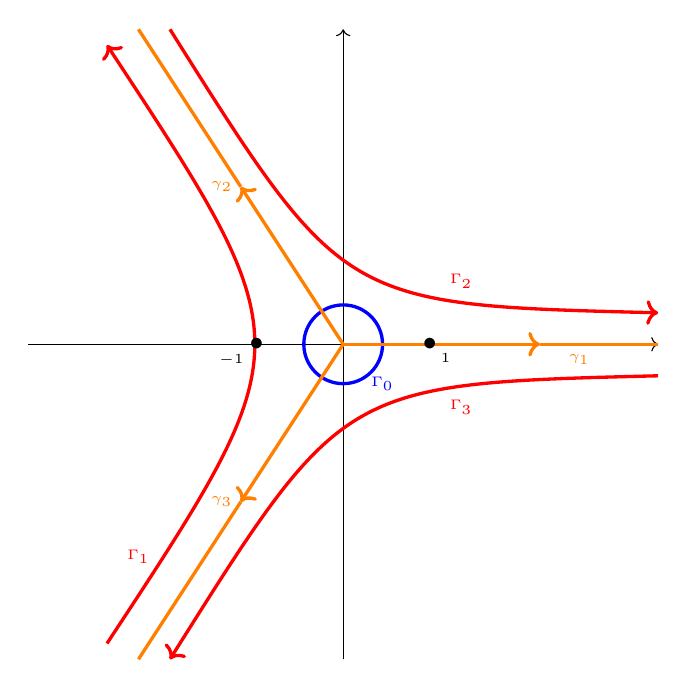
\begin{tikzpicture}
    \draw[->] (4,0)--(4,8);
    \draw[->] (0,4)--(8,4);
    \draw[blue,very thick] (4,4) circle (0.5) ;
    \node[blue,font=\tiny] at (4.5,3.5) {$\Gamma_0$};
    \node[red,font=\tiny] at (1.4,1.3) {$\Gamma_1$};
    \draw[red,very thick,->] (1,0.2) .. controls (3.5,4) .. (1,7.8);
    \node[red,font=\tiny] at (5.5,4.8) {$\Gamma_2$};
    \draw[red,very thick,->] (1.8,8) .. controls (4,4.5) ..(8,4.4) ;
     \node[red,font=\tiny] at (5.5,3.2) {$\Gamma_3$};
    \draw[red,very thick,->] (8,3.6) .. controls (4,3.5) ..(1.8,0) ;
    \draw[orange,very thick,->] (4,4)--(6.5,4);
    \draw[orange,very thick] (6.5,4)--(8,4);
    \node[orange,font=\tiny,below] at (7,4) {$\gamma_1$};
    \draw[orange,very thick,->] (4,4)--(2.7,6);
    \draw[orange,very thick] (2.7,6)--(1.4,8);
    \node[orange,font=\tiny,right] at (2.2,6) {$\gamma_2$};
    \draw[orange,very thick,->] (4,4)--(2.7,2);
    \draw[orange,very thick] (2.7,2)--(1.4,0);
    \node[orange,font=\tiny,right] at (2.2,2) {$\gamma_3$};
    \node at (5.1,4) {$\bullet$};
    \node at (2.9,4) {$\bullet$};
    \node[font=\tiny,below,right] at (2.3,3.8) {$-1$};
    \node[font=\tiny,below] at (5.3,4) {$1$};
    \end{tikzpicture}
    \caption{Representation of the path of integration for $\mathrm{A}_k,\mathrm{B}_0,\mathrm{B}_k$ respectively in red, blue and orange.}\label{fig:path-generalized-Airy}
\end{figure}

Each generalized Airy function is a solution of
\begin{equation}
\left[\partial_y^3-y\partial_y+(p-1)\right]f=0
\end{equation} 
and if $p=0$ they reduce to the classical Airy functions.

Following the treatment of the Airy--Lucas functions, we'll rewrite the generalized Airy function $\mathrm{A}_1(y,p)$ as thimble integrals with the function $f=4u^3-3u$. This follows from the change of coordinates $z=\tfrac{2}{3}y^{3/2}$, and gives $\mathrm{A}_1(y,p) = (12 z)^{\tfrac{1-p}{3}}\, I_+(z,p)$ with 
%
\[I_+(z,p):=\frac{1}{2\pi i}\int_{z^{-1/3}\Gamma_1} e^{-z(4u^3-3u)} \frac{du}{u^p}\]
%
\begin{verify}
  \begin{align*}
I_{+}(z,p)&=\frac{1}{2\pi i}\int_{\Lambda_{+}}e^{-z(4u^3-3u)}\, \frac{du}{u^p} &\\
&=\frac{1}{2\pi i}(12 z)^{(p-1)/3}\int_{z^{1/3}\Lambda_{+}}e^{-z(\tfrac{4}{12}\tfrac{t^3}{z}-3 (12 z)^{-1/3}t)}\frac{dt}{t^p} & u=(12 z)^{-\tfrac{1}{3}}t\\
&=\frac{1}{2\pi i}(12 z)^{(p-1)/3}\int_{z^{1/3}\Lambda_{+}}e^{-\left(\frac{t^3}{3}-(\tfrac{3}{2} z)^{2/3}t\right)}\frac{dt}{t^p} & \\
&=(12 z)^{(p-1)/3}\mathrm{A}_1((\tfrac{3}{2}z)^{2/3},p)
\end{align*}  
\end{verify}
%
Notice that, the critical points of $f$ are $\alpha_{\pm}=\pm\tfrac{1}{2}$, as in the Airy case. However, the volume form $\nu_p$ is meromorphic, hence $f$ should be regarded as a function from $\C^*$ to $\C$. In particular, in this example we'll see that there is a new singularity at the origin due to the singularity of $\nu_p$. For simplicity, we'll restrict to the case $p=1$. Then, $I_+(z,1)$ solves
\begin{equation}\label{eq:I}
\left[\partial_z^3-\partial_z+\frac{1}{z}\partial_z^2-\frac{1}{9}\frac{\partial_z}{z^2}\right]\varphi=0
\end{equation}
or equivalently, $\partial_z\varphi$ solves the modified Bessel equation \eqref{eqn:mod-bessel-AL} with parameter $1/3$. Therefore, following the reasoning of Section \ref{big-idea} and the results of Sections \ref{pos-root-AL} and \ref{neg-root-AL}, we get two analytic solutions of \eqref{eq:I}: $\laplace_{\zeta,1}v_{1,1}$ and $\laplace_{\zeta,-1}v_{-1,1}$ 
\[ v_{1,1}=-i\sqrt{2}\, (\zeta_1+1)^{-1}\, \zeta_1^{-1/2}\, {}_2F_1\Big(\tfrac{1}{6},\tfrac{5}{6};\tfrac{1}{2};-\tfrac{1}{2}\zeta_{1}\Big)\]
\[ v_{-1,1}=-\sqrt{2}\, (1-\zeta_{-1})^{-1}\, \zeta_{-1}^{-1/2}\, {}_2F_1\Big(\tfrac{1}{6},\tfrac{5}{6};\tfrac{1}{2};\tfrac{1}{2}\zeta_{-1}\Big)\]
where $\zeta_1=\zeta-1$ and $\zeta_{-1}=\zeta+1$. 
\begin{verify}
From the result about the Bessel equation, we know there exists two analytic functions $v_1$ and $v_{-1}$ such that $\varphi_1$ and $\varphi_2$ defined by $\partial_z\varphi_1=\laplace_{\zeta,1}v_1$ and $\partial_z\varphi_2=\laplace_{\zeta,-1}v_{-1}$, give a frame of analytic solutions of \eqref{eq:I}. Then we argue as follows:
\begin{align*}
    \partial_z\varphi_1&=\laplace_{\zeta,1}v_1\\
    \varphi_1-\varphi_1(a)&=\int_a^z\int_1^{\infty}e^{-y\zeta} v_1 d\zeta \, dy\\
    &=\int_1^{\infty}d\zeta\,  v_1 \, \int_a^ze^{-y\zeta}  \, dy\\
    &=\int_1^{\infty}d\zeta\,  v_1 \, \Big[\frac{e^{-\zeta a}}{\zeta}-\frac{e^{-z\zeta}}{\zeta}\Big]\\
    &=\laplace_{\zeta,1} \tfrac{v_1}{\zeta}-\Big[\laplace_{\zeta,1}\tfrac{v_1}{\zeta}\Big](a)
\end{align*}
\end{verify}
Notice that $v_{1,1}\in\singexpalg{1/2}(\Omega_1)$, it has a simple pole at $\zeta_1=-1$ and it is a log--singularity at $\zeta_1=-2$. Similarly, $v_{-1,1}\in\singexpalg{1/2}(\Omega_{-1})$, it has a simple pole at $\zeta_{-1}=1$ and it is a log--singularity at $\zeta_{-1}=2$.

Notice that $\laplace_{\zeta,1}v_{1,1}$ and $\laplace_{\zeta,-1}v_{-1,1}$ are not a frame of solutions; the equation \eqref{eq:I} is of degree three, but it is enough to consider the constant function $1=\laplace_\zeta \delta$ to build a frame of analytic solutions, where $\delta$ is the formal unit (see the definition in Section \ref{convolution}). In particular, $1=B_0(z,1)$ and confirms Borel regularity for the constant solution. 
%
\color{RoyalBlue}
\subsubsection{Thimble projection formula}
In Theorem \ref{thm:maxim-dim}, we proved a $3/2$-derivative formula to compute the Borel transform of the asymptotics of a thimble integral.
\color{black}
\subsection{Third-order thimble integrals}
Let $f\colon\C\to \C$ be a degree three polynomial\footnote{Every degree three polynomial $a_3 u^3+a_2 u^2+a_1 u+a_0$ can be written in the form $a_3u^3+pu+q$, after a change of coordinates $u\to u-\frac{a_2}{3 a_3}$. Furthermore, we can restrict to monic polynomials by setting $a_3=1$.}, we are going to consider thimble integrals of the form 

\[ I_j(z) = \int_{\Lambda_j} \exp\left[z\big(u^3 + pu + q)\right]\,du \]

where $\Lambda_j$ is a thimble in $H_{1}^{B,z}$ through a critical point of $f$. We can distinguish between the case when $f$ has two distinct critical points $x_+, x_-$ and only one critical point $x$, which correspond respectively to the case $p\neq 0$ and $p=0$. \footnote{Equivalently, the difference between the generic case ($p\neq 0$) and the degenerate one ($p=0$) is visible from the ODE perspective as in the former case $I$ is a solution of degree two ODE \[\left[\partial_z^2 +2q \partial_z+\left(\frac{4p^3}{27}+q^2\right)+\frac{1}{z}\left(\partial_z +q \right)-\frac{1}{9z^2}\right]\Phi=0,\] while in the latter, $I$ solves a degree one ODE (see \eqref{eqn:degree-3-poly-1root}).}
Recall that translations and scaling-rotations act naturally on the image of $f\colon X\to \C$ ($f$ not necessarily a degree three polynomial), and their action transforms the thimble integral $I_j$ in the following ways:
\begin{itemize}
    \item \textbf{Action of translations:} let $q\in\C$, post-composing with translation of $q$ maps $f\to f+q$, thus 
    \begin{align*}
        \int_{\Lambda_j}e^{z (f+q)} \nu &= e^{qz} I_j(z)
    \end{align*}
    \item  \textbf{Action of scaling-rotations:} let $\gamma\in\C$, post-composing with scaling-rotations by $\gamma$ maps $f\to \gamma\cdot f$, thus 
    \begin{align*}
        \int_{\Lambda_j}e^{z (\gamma\cdot f)} \nu &= I_j(z \gamma)
    \end{align*}
\end{itemize}
In particular, we can always reduce to study the thimble integral in simpler situations. 
As an example, every degree three polynomial with distinct critical points can be transformed in the Chebyshev polynomial $T_3(t)=4 t^3-3t$, implying that the thimble integral $I_+$ can be transformed into the Airy--Lucas integral with parameter $m=1, n=3$. This follows by post-composing $f$ with a translation of $-q$ followed by a scaling-rotation of $\frac{ -i 3^{3/2}}{2 p^{3/2}}$
\begin{align*}
    f-q &= u^3 + pu \\
    (f-q) \cdot \frac{ -i 3^{3/2}}{2 p^{3/2}} &= 4 \Big(\sqrt{-\tfrac{3}{p}} \tfrac{u}{2} \Big)^{3} - 3\Big(\sqrt{-\tfrac{3}{p}} \tfrac{u}{2} \Big) \\
    &= 4 t^3- 3t 
\end{align*}
with $t= \sqrt{-\frac{3}{p}} \frac{u}{2}$. Then the thimble integral $I_+$ gets transformed into 
\begin{align*}
    e^{-zq} I_+\left(-\tfrac{i 3^{3/2}}{2 p^{3/2}} z\right)&= \int_{\Lambda_+} e^{z (4t^3-3t)} du\\
    &= 2\sqrt{-\tfrac{p}{3}} \int_{\Lambda_+} e^{z (4t^3-3t)} dt \\
    &= 2\sqrt{-\tfrac{p}{3}} K_{1/3}(z). 
\end{align*}
In particular, when $p\neq 0$, the thimble integral $I_+$ can be studied following the analysis of Appendix \ref{airy-appendix}. 
%In both cases, we’ll compute the differential equation satisfied by $I$. 

%\begin{lemma}
 %Let $f(u)=u^3+pu+q$, 
  %  \begin{itemize}
   %     \item if $p\neq 0$, then $I_{\pm}(z)$ solves 
    %    \begin{equation}\label{eqn:degree-3-poly-2roots}
    %        \left[\partial_z^2 +2q \partial_z+\left(\frac{4p^3}{27}+q^2\right)+\frac{1}{z}\left(\partial_z +q \right)-\frac{1}{9z^2}\right]\Phi=0
    %    \end{equation}
    %    \item  if $p=0$, then $I(z)$ solves
     %   \begin{equation}\label{eqn:degree-3-poly-1root}
      %      \left[\partial_z+q+\frac{1}{3z}\right]I=0
      %  \end{equation}
    %\end{itemize}
%\end{lemma}
%\begin{proof}
 %   The proof follows from a direct computation. 
%\end{proof}

%Let us first assume $p\neq 0$, then $x_{\pm}=\pm\sqrt{-p/3}$ and the critical values are $\alpha_{\pm}=f(x_\pm)$. Notice that equation \eqref{eqn:degree-3-poly-2roots} admits slight solutions as $\tau_\pm=\frac{1}{2}$ (recall the definition of $\tau\pm=\frac{Q(-\alpha_\pm)}{P'(-\alpha_\pm)}$ as in Section \ref{borel_reg-ODE}), thus, for $\theta=-\arg z$, $\laplace_{\zeta,f(\alpha_\pm)}^{\theta}v_\pm$ solves \eqref{eqn:degree-3-poly-2roots} if and only $v_\pm$ solves   

%\begin{equation}\label{eqn:deg3-borel-ODE}
 %   \left[\Big[\zeta^2-2q\zeta+\big(\frac{4p^3}{27}+q^2\big)\Big]\partial_\zeta^2+3(\zeta-q)\partial_\zeta+\frac{8}{9}\right]v_\pm=0
%\end{equation}

%Let us find a solution of \eqref{eqn:deg3-borel-ODE} slight at $\zeta=\alpha_+$: in the new coordinate $\zeta_+:=\zeta-\alpha_+$, equation \eqref{eqn:deg3-borel-ODE} becomes

%\begin{equation*}
 %   \left[\zeta_+ (\zeta_+ + \frac{4}{3}p\, x_+)\partial_{\zeta_+}^2+ \left[2p\, x_++3\zeta_{+}\right]\partial_{\zeta_+} +\frac{8}{9} \right]v_+=0
%\end{equation*}

%which is an hypergeometric equation in the coordinate $\xi=-\frac{3}{4p\,x_+}\zeta_+$

%\begin{equation*}
 %   \left[\xi (1-\xi)\partial_{\xi}^2+ 3\big(\frac{1}{2}-\xi\big)\partial_{\xi}-\frac{8}{9} \right]v_+=0
%\end{equation*}

%and it admits a slight solution \textcolor{red}{the solution should match with the one of airy, so choose $w_2$ in DLMf list and not $w_1$}

%\begin{align*}
 %   v_+ &= \xi^{-1/2}\, {}_2F_1\left(\frac{1}{6},\frac{5}{6} ;\frac{3}{2};1-\xi\right)\\
  %  &=\left(\frac{3}{4p\,x_+}\zeta_+\right)^{-1/2}\, {}_2F_1\left(\frac{1}{6},\frac{5}{6} ;\frac{3}{2};1-\frac{3}{4p\,x_+}\zeta_+\right). 
%\end{align*}

%Notice that $v_+$ is a hypergeometric function with the same parameters as the hypergeometric function $v_1$ in the example of Airy \S \ref{pos-root}. Similarly for $\zeta_-=\zeta-\alpha_-$ 

%\begin{equation*}
%    v_- =\left(\frac{3}{4p\,x_-}\zeta_-\right)^{-1/2}\, {}_2F_1\left(\frac{1}{6},\frac{5}{6} ;\frac{3}{2};1-\frac{3}{4p\,x_-}\zeta_-\right). 
%\end{equation*}
We then consider the case when $p=0$, and we study it both as a solution of an ODE and as a thimble integral.
First, notice that $I(z)$ solves
       \begin{equation}\label{eqn:degree-3-poly-1root}
          \left[\partial_z+q+\frac{1}{3z}\right]I=0
       \end{equation}
and we can find a Borel regular solution following the argument of Section~\ref{big-idea}: $\laplace_{\zeta,\alpha}^{\theta}v$ is a solution of \eqref{eqn:degree-3-poly-1root} if and only if $v$ is a solution of 
\begin{align*}
   \left[ (\zeta-q)\partial_\zeta +\frac{2}{3}\right] v=0
\end{align*}
namely $v=(\zeta-q)^{-2/3}=\zeta_q^{-2/3}={}_2F_1\left(a,\frac{2}{3};a;1-\zeta_q\right)$, where $\zeta_q=\zeta-q$ and $a\in\C$ is a free parameter. 

The result is confirmed by the thimble projection reasoning which in this simple case reads
\begin{align*}
    \int_{\Lambda} e^{-z (u^3+q)} du &= e^{-zq} e^{i\pi/3} \int_0^{+e^{i\theta}\infty} e^{-z\zeta} \zeta^{-2/3} d\zeta\\
    &= e^{i\pi/3} \int_q^{+e^{i\theta}\infty} e^{-z\zeta} \, \zeta_q^{-2/3}\,  d\zeta
\end{align*}
where $e^{\pi i/3}$ accounts for the monodromy of $\zeta^{-2/3}$ at the origin. 
\begin{remark}
    The degenerate case $p=0$ can be recovered from the generic case, taking the limit of $I_+(z)$ as $p\to 0$. Indeed, 
    \[ e^{-zq} I_+(z)=2 \sqrt{-\frac{p}{3}} K_{1/3}\Big(\frac{2p^{3/2}}{i3^{3/2}}z\Big)\]
    and its limit as $p\to 0$ can be computed from equations 10.25.2 and 10.27.4 in \cite{dlmf} giving 
    \[ e^{\pi i/3} \Gamma\big(\tfrac{1}{3}\big) e^{-zq} z^{-1/3}.  \]
    \begin{verify}
        \begin{align*}
            2\sqrt{\frac{-p}{3}} K_{1/3}\Big(\frac{2ip^{3/2}}{3^{3/2}}z\Big)&=2\sqrt{\frac{-p}{3}}\left[\frac{\pi}{2\sin(\pi/3)}\Big(I_{-1/3}\big(\tfrac{2ip^{3/2}}{3^{3/2}}z\big)-I_{1/3}\big(\tfrac{2ip^{3/2}}{3^{3/2}}z\big)\Big)\right]\\
            &=\frac{2}{3}\pi ip^{1/2}\left[\Big(\frac{ip^{3/2}}{3^{3/2}}z\Big)^{-1/3}\sum_{k\geq 0}\frac{(-\tfrac{p^3}{3}z^2)^k}{k!\Gamma(k+\tfrac{2}{3})}-\Big(\frac{ip^{3/2}}{3^{3/2}}z\Big)^{1/3}\sum_{k\geq 0}\frac{(-\tfrac{p^3}{3}z^2)^k}{k!\Gamma(k+\tfrac{4}{3})}\right]\\
            &=\frac{2\pi}{\sqrt{3}} e^{\pi i/3} z^{-1/3} \sum_{k\geq 0}\frac{(-\tfrac{p^3}{3}z^2)^k}{k!\Gamma(k+\tfrac{2}{3})}-\frac{2\pi }{3\sqrt{3}} e^{2\pi i/3} z^{1/3} p \sum_{k\geq 0}\frac{(-\tfrac{p^3}{3}z^2)^k}{k!\Gamma(k+\tfrac{4}{3})}
        \end{align*}
         Now we take the limit as $p\to 0$ and we find 
         \[\frac{2\pi}{\sqrt{3}} e^{\pi i/3} z^{-1/3} \frac{1}{\Gamma\big(\tfrac{2}{3}\big)}=e^{\pi i/3} \Gamma\big(\tfrac{1}{3}\big) z^{-1/3}\]
    \end{verify}
    From the properties of the Laplace transform, we then deduce
    \[e^{\pi i/3} \Gamma\big(\tfrac{1}{3}\big) e^{-zq} z^{-1/3}= e^{\pi i/3} e^{-qz} \laplace_{\zeta,0}(\zeta^{-2/3}) = e^{\pi i/3} \laplace_{\zeta_{-q},q}(\zeta^{-2/3})\]
    which agrees with the thimble integral representation of $I$ computed above. 
\end{remark}
\subsection{The triangular catilever}\label{sec:catilever}
The equation of a triangular cantilever with \textcolor{orange}{[...]} $\mu\in\R\setminus\{0\}$ is 
\begin{equation}\label{eqn:triangular_cantilever}
    \Big[\big[\Big(\frac{\partial}{\partial z}\Big)^4 +\mu\big]+\frac{2}{z}\Big(\frac{\partial}{\partial z}\Big)^3\Big]\varphi=0 .
\end{equation}
Going to the position domain we can solve the equation explicitly: let $\alpha_1,\ldots,\alpha_4$ be the solutions of $\lambda^4+\mu=0$; we'll look for solutions $v_j$ whose Laplace transform $\laplace_{\zeta,\alpha_j}v_j$ satisfies the equation \eqref{eqn:triangular_cantilever}. For $j=1,\ldots,4$, $v_j$ solves
\begin{equation}\label{eqn:position_j}
    \Big[\big[\zeta^4+\mu\big]+2\fracderiv{-1}{\zeta}{\alpha_j}\circ(-\zeta)^3\Big] v_j=0
\end{equation}
As we'll show in Section \ref{shifting}, for $j=1,\ldots,4$, $v_j$ solves \eqref{eqn:position_j} if and only if $v_j$ solves the differential equation 
\begin{equation}
    \Big[\big[\zeta^4+\mu\big]\tfrac{\partial}{\partial\zeta}-2\zeta^3\Big]v_j = 0
\end{equation}
In particular, at $\zeta_j=\zeta-\alpha_j$ we find 
\[v_j \propto \frac{1}{\zeta_j^{1/2}}\, \prod_{k\neq j}(\zeta_j-\alpha_k+\alpha_j)^{-1/2}.\]
\textcolor{orange}{[Stokes? Thimbles?]}
%\subsection{The anharmonic oscillator}\label{sec:anharmonic_oscillator}

\appendix

\section{The Airy equation}\label{airy-appendix}

\subsubsection{Rewriting as a modified Bessel equation}
We can distill the most interesting part of the Airy function by writing
\[ \Ai(y) = \tfrac{1}{\pi\sqrt{3}}\,y^{1/2}\,K\big(\tfrac{2}{3} y^{3/2}\big), \]
where
\begin{equation}\label{integral:mod-bessel}
K(z) = i\sqrt{3} \int_{z^{-1/3}\Lambda_1} \exp\left[z \left(4u^3 - 3u\right)\right]\,du.
\end{equation}
and the contour $\Lambda_1$ is represented in Figure \ref{fig:path_Airy}.
Saying that $\Ai$ satisfies the Airy equation is equivalent to saying that $K$ satisfies the modified Bessel equation
\begin{equation}\label{eqn:mod-bessel-1/3}
\left[z^2 \big(\tfrac{\partial}{\partial z}\big)^2 + z \tfrac{\partial}{\partial z} - \big[\big(\tfrac{1}{3}\big)^2 + z^2\big]\right] K = 0.
\end{equation}
In fact, $K$ is the modified Bessel function $K_{1/3}$~\cite[equation~9.6.1]{dlmf}.
%The method we'll demonstrate in Section~\ref{spatial} works for any differential equation
%\[ \left[ P\big(\tfrac{\partial}{\partial z}\big) + z^{-1} Q\big(\tfrac{\partial}{\partial z}\big) + z^{-2} R(z^{-1}) \right] \varphi = 0, \]
%where $P$ is a polynomial, $Q$ is a polynomial of one degree lower, and $R$ is an entire function.
Like we did in equation~\eqref{eqn:reg-mod-bessel-AL}, we can rewrite the modified Bessel equation above as 

\begin{equation}\label{eqn:reg-mod-bessel}
\left[ \big[ \big(\tfrac{\partial}{\partial z}\big)^2 - 1 \big] + z^{-1} \tfrac{\partial}{\partial z} - \big(\tfrac{1}{3}\big)^2 z^{-2} \right] K = 0.
\end{equation}

\subsection{Asymptotic analysis}
From the general theory of ODE of Poincar\'e rank $1$, we know that the space of trans-series solutions of ~\eqref{eqn:reg-mod-bessel} has a basis of trans-monomials
\[ \{ e^{-\alpha z} z^{-\tau_\alpha}\,\series{W}_\alpha \mid \alpha^2 - 1 = 0 \} \]
where the $\series{W}_\alpha\in\C\llbracket z^{-1} \rrbracket$ are formal power series in $z^{-1}$. From equations 10.40.2 and 10.17.1 of \cite{dlmf}, we learn that $K \sim \left(\tfrac{\pi}{2}\right)^{1/2} e^{-z} z^{-1/2}\,\series{W}_1$, with
\begin{equation}\label{bessel-asymp}
\series{W}_1 = 1 - \frac{(\tfrac{1}{6})_1 (\tfrac{5}{6})_1}{2^1 \cdot 1!}\;z^{-1} + \frac{(\tfrac{1}{6})_2 (\tfrac{5}{6})_2}{2^2 \cdot 2!}\;z^{-2} - \frac{(\tfrac{1}{6})_3 (\tfrac{5}{6})_3}{2^3 \cdot 3!}\;z^{-3} + \ldots
\end{equation}
The holomorphic analysis in Section~\ref{spatial} will give us holomorphic solutions
\[ \{ e^{-\alpha z} z^{-\tau_\alpha}\,W_\alpha \mid \alpha^2 - 1 = 0 \}, \]
which seem analogous to the trans-monomials above. Borel summation makes the analogy precise. We’ll see in Section~\ref{bessel-regularity} that each $z^{-\tau_\alpha}\,W_\alpha$ is proportional to the Borel sum of $z^{-\tau_\alpha}\,\series{W}_\alpha$. This is an evidence of \cite[Theorem~4]{reg-sing-volterra}.

\subsection{Building a distinguished frame of analytic solutions}
\subsubsection{Going to the spatial domain}\label{spatial}
%\subsubsection{The big idea}\label{big-idea}
We are going to look for functions $v_j$ whose Laplace transforms $\laplace_{\zeta, \alpha_j} v_j$ satisfy equation~\eqref{eqn:reg-mod-bessel}. We’ll succeed when $\alpha^2 - 1 = 0$, and we’ll see that $K$ is a scalar multiple of $\laplace_{\zeta, 1} v_1$.

We can see from Section~\ref{L-int-op} that $\laplace_{\zeta, \alpha} v$ satisfies the differential equation~\eqref{eqn:reg-mod-bessel} if and only if $v$ satisfies the integral equation
\begin{equation}\label{int-eq:spatial-mod-bessel}
\left[ \big[ \zeta^2 - 1 \big] - \fracderiv{-1}{\zeta}{\alpha} \circ \zeta - \big(\tfrac{1}{3}\big)^2 \fracderiv{-2}{\zeta}{\alpha} \right] v = 0.
\end{equation}
It's tempting to differentiate both sides of this equation until we get
\begin{equation}\label{diff-eq:spatial-mod-bessel}
\left[ \big(\tfrac{\partial}{\partial \zeta}\big)^2 \circ \big[ \zeta^2 - 1 \big] - \tfrac{\partial}{\partial \zeta} \circ \zeta - \big(\tfrac{1}{3}\big)^2 \right] v = 0,
\end{equation}
which is easier to solve. However, as we learned in Section~\ref{shifting}, a solution of equation~\eqref{diff-eq:spatial-mod-bessel} satisfies equation~\eqref{int-eq:spatial-mod-bessel} if it's slight and locally integrable at $\zeta = \alpha$. 

This is great news, because equation~\eqref{diff-eq:spatial-mod-bessel} has a regular singularity at each root of $\zeta^2 - 1$, and the Frobenius method often gives a slight solution at each regular singular point. We can see the regular singularities by moving the derivatives to the right:
\[ \left[ (\zeta^2 - 1) \big(\tfrac{\partial}{\partial \zeta}\big)^2 + 3\zeta \tfrac{\partial}{\partial \zeta} + \big[ 1 - \big(\tfrac{1}{3}\big)^2 \big] \right] v = 0. \]
In Sections \ref{pos-root}\,--\,\ref{neg-root}, we’ll see this approach succeed. For each root $\alpha$, we'll find a solution $v_\alpha$ of equation~\eqref{diff-eq:spatial-mod-bessel} which is slight and locally integrable at $\zeta = \alpha$. We know the function $\laplace_{\zeta, \alpha} v_\alpha$ will satisfy equation~\eqref{eqn:reg-mod-bessel}, and we can even find its asymptotics from the order $\tau_\alpha$ of $v_\alpha$. We learned in Section~\ref{translation} that
\[ \laplace_{\zeta, \alpha} v_\alpha = e^{-\alpha z} V_\alpha \]
where $V_\alpha = \laplace_{\zeta_\alpha, 0} v_\alpha$ and $\zeta = \alpha + \zeta_\alpha$. We can see from Section~\ref{sec:reg-decay} that $V_\alpha$ is asymptotic to a scalar multiple of $z^{ - \tau_\alpha}$ at $z = \infty$, so the further decomposition
\[ \laplace_{\zeta, \alpha} v_\alpha = e^{-\alpha z} z^{-\tau_\alpha} W_\alpha, \]
makes $W_\alpha$ is asymptotic to a scalar multiple of $1+O(z^{-1})$ at $z = \infty$.
%\textcolor{Magenta}{Show that $W_1$ is asymptotic to $\tilde{W}_1$!}
%\color{Peru}
%\begin{align*}
%\left[ \big(\tfrac{\partial}{\partial \zeta}\big)^2 \circ (\zeta - 1)(\zeta + 1) - \tfrac{\partial}{\partial \zeta} \circ \zeta - \big(\tfrac{1}{3}\big)^2 \right] v & = 0
%\end{align*}
%\color{Sienna}
%\begin{align*}
%\left[ \big[ 2 + 2(2\zeta) \tfrac{\partial}{\partial \zeta} + (\zeta^2 - 1) \big(\tfrac{\partial}{\partial \zeta}\big)^2 \big] - \big[ 1 + \zeta \tfrac{\partial}{\partial \zeta} \big] - \big(\tfrac{1}{3}\big)^2 \right] v & = 0 \\
%\left[ (\zeta^2 - 1) \big(\tfrac{\partial}{\partial \zeta}\big)^2 + 3\zeta \tfrac{\partial}{\partial \zeta} + \big[ 1 - \big(\tfrac{1}{3}\big)^2 \big] \right] v & = 0 \\
%\left[ (\zeta - 1)(\zeta + 1) \big(\tfrac{\partial}{\partial \zeta}\big)^2 + 3\zeta \tfrac{\partial}{\partial \zeta} + \big[ 1 - \big(\tfrac{1}{3}\big)^2 \big] \right] v & = 0
%\end{align*}
%\color{black}
%%In terms of the coordinate $\zeta_\alpha$ with $\zeta = \alpha + \zeta_\alpha$, this equation is written
%%\begin{equation}\label{eqn:centered-mod-bessel}
%%\[ \left[ \big[ \zeta_\alpha (\zeta_\alpha + 2\alpha) + \alpha^2 - 1 \big] + \fracderiv{-1}{\zeta_\alpha}{0} \circ \big[ \zeta_\alpha + \alpha \big] - \big(\tfrac{1}{3}\big)^2 \fracderiv{-2}{\zeta_\alpha}{0} \right] w = 0. \]
%%\end{equation}
\subsubsection{Focus on $\zeta = 1$}\label{pos-root}
Let's find a solution of equation~\eqref{diff-eq:spatial-mod-bessel} which is slight and locally integrable at $\zeta = 1$. Define a new coordinate $\zeta_1$ on $\C$ so that $\zeta = 1 + \zeta_1$. In this coordinate, equation~\eqref{diff-eq:spatial-mod-bessel} looks like
\begin{equation}%%\label{diff-eq:spatial-mod-bessel-pos}
\left[\zeta_1(2 + \zeta_1) \big(\tfrac{\partial}{\partial \zeta_1}\big)^2 + 3(1 + \zeta_1) \tfrac{\partial}{\partial \zeta_1} + \big[1 - \big(\tfrac{1}{3}\big)^2\big]\right] v = 0.
\end{equation}
With another change of coordinate, given by $\zeta_1 = -2\xi_1$, we can rewrite equation~\eqref{diff-eq:spatial-mod-bessel} as the hypergeometric equation
\begin{equation}\label{diff-eq:hypergeom-pos}
\left[\xi_1 (1 - \xi_1) \big(\tfrac{\partial}{\partial \xi_1}\big)^2 + 3(\tfrac{1}{2} - \xi_1) \tfrac{\partial}{\partial \xi_1} - \big[1 - \big(\tfrac{1}{3}\big)^2\big]\right] v = 0.
\end{equation}
Looking through the twenty-four expressions for Kummer's six solutions, we find one \cite[formula~15.10.12]{dlmf} which is manifestly slight and locally integrable at $\xi_1 = 0$:
\begin{alignat*}{2}
v_1 &=\;& \hphantom{-i\sqrt{2}}\,\xi_1^{-1/2} & {}_2F_1\big(\tfrac{1}{6}, \tfrac{5}{6}; \tfrac{1}{2}; \xi_1\big) \\
&=\;& -i\,\left(\frac{\zeta_1}{2}\right)^{-1/2} & {}_2F_1\big(\tfrac{1}{6}, \tfrac{5}{6}; \tfrac{1}{2}; -\tfrac{1}{2}\zeta_1\big)
\end{alignat*}
From the argument in Section~\ref{spatial}, we know that $\laplace_{\zeta, 1} v_1$ satisfies equation~\eqref{eqn:reg-mod-bessel}, and can be written as $e^{-z} V_1$, where $V_1 = \laplace_{\zeta_1, 0} v_1$. Since $v_1$ has order $-1/2$, the decomposition $V_1 = z^{1/2} W_1$ makes $W_1$ asymptotic to a scalar multiple of $z^{-1}$ at $z = \infty$.
\subsubsection{Focus on $\zeta = -1$}\label{neg-root}
Let's find a solution of equation~\eqref{diff-eq:spatial-mod-bessel} which is slight and locally integrable at $\zeta = -1$. In the rescaled coordinate from Section~\ref{pos-root}, this is the point $\xi_1 = 1$. Looking again through Kummer's table of solutions, we find another expression \cite[formula~15.10.14]{dlmf} which is manifestly slight and locally integrable at $\xi_1 = 1$:
\begin{alignat*}{2}
v_{-1} &=\;& (1-\xi_1)^{-1/2} & F\big(\tfrac{1}{6}, \tfrac{5}{6}; \tfrac{1}{2}; 1-\xi_1\big) \\
&=\;& \left(\frac{\zeta_{-1}}{2}\right)^{-1/2} & F\big(\tfrac{1}{6}, \tfrac{5}{6}; \tfrac{1}{2}; \tfrac{1}{2}\zeta_{-1}\big)
\end{alignat*}
where $\zeta_{-1}$ is the coordinate with $\zeta = -1 + \zeta_{-1}$. From the argument in Section~\ref{big-idea}, we know that $\laplace_{\zeta, -1} v_{-1}$ satisfies equation~\eqref{eqn:mod-bessel}, and can be written as $e^z V_{-1}$, where $V_{-1} = \laplace_{\zeta_{-1}, 0} v_{-1}$. Since $v_{-1}$, like our other solution, has order $-1/2$, the same decomposition $V_{-1} = z^{1/2} W_{-1}$ makes $W_{-1}$ asymptotic to a scalar multiple of $z^{-1}$ at $z = \infty$.

In this example, $v_1$ and $v_{-1}$ happen to be related by a symmetry: the M\"{o}bius transformation that pulls $\zeta$ back to $-\zeta$. Kummer's solutions typically come from six different hypergeometric equations, which are related by the M\"{o}bius transformations that permute their singularities. In our case, though, exchanging $1$ with $-1$ keeps equation~\eqref{diff-eq:spatial-mod-bessel} the same.
%\color{DodgerBlue}
%If we follow the routine from Section~\ref{pos-root}, rewriting equation~\eqref{diff-eq:spatial-mod-bessel} in the coordinate $\zeta_{-1}$ and then rewriting it again in a more recognizable form, we arrive at the hypergeometric equation
%\[ \left[\xi_{-1} (1 - \xi_{-1}) \big(\tfrac{\partial}{\partial \xi_{-1}}\big)^2 + 3(\tfrac{1}{2} - \xi_{-1}) \tfrac{\partial}{\partial \xi_{-1}} - \big[1 - \big(\tfrac{1}{3}\big)^2\big]\right] v = 0, \]
%where $\zeta_{-1} = 2\xi_{-1}$. This is the same as what we get by substituting $\xi_{-1}$ for $\xi_1$ in Section~\ref{pos-root}! In other words, the holomorphic map that pulls $\xi_{-1}$ back to $\xi_1$.
\subsection{Borel regularity}\label{bessel-regularity}
Recall that $\tilde{W}_1$ is a formal solution of \eqref{eqn:reg-mod-bessel}
\begin{equation}
\tilde{W}_1(z)=\sum_{n=0}^{\infty}\frac{\left(\frac{1}{6}\right)_n\left(\frac{5}{6}\right)_n}{n!}\frac{(-1)^n}{2^n}z^{-n}.
\end{equation}
Our goal is to prove that the Borel sum of $z^{-1/2}\tilde{W}_1$ is proportional to $V_1=\laplace_{\zeta_1,0}v_1$. 
%
%\subsubsection{Borel sum of $\tilde{W}_1$}
%
%Let us first compute the Borel transform of $\tilde{W}_1$:
%
%
%\begin{align*}
%\tilde{w}_1(\zeta)&=\delta+\sum_{n=1}^{\infty}\frac{\left(\frac{1}{6}\right)_n\left(\frac{5}{6}\right)_n}{n!}\frac{(-1)^n}{2^n}\frac{\zeta^{n-1}}{\Gamma(n)}\\
%&=\delta -\frac{1}{2}\sum_{n=0}^{\infty}\frac{\left(\frac{1}{6}\right)_{n+1}\left(\frac{5}{6}\right)_{n+1}}{\Gamma(n+2)n!}\frac{(-\zeta)^n}{2^n}\\
%&=\delta-\frac{1}{2}\frac{\Gamma(\frac{7}{6})\Gamma(\frac{11}{6})}{\Gamma(\frac{1}{6})\Gamma(\frac{5}{6})}\sum_{n=0}^{\infty}\frac{\left(\frac{7}{6}\right)_{n}\left(\frac{11}{6}\right)_{n}}{\Gamma(n+2)n!}\frac{(-\zeta)^n}{2^n}\\
%&=\delta-\frac{5}{72}\,\, {}_2F_1\left(\frac{7}{6},\frac{11}{6};2,-\frac{\zeta}{2}\right)
%\end{align*}
Let us compute the Borel transform of $z^{-1/2}\tilde{W}_1$: notice that the appropriate coordinate is $\zeta_1$ 
\begin{align*}
\borel\left[z^{-1/2}\tilde{W}_1(z)\right](\zeta_1)&=\borel\left[\sum_{n=0}^{\infty}\frac{\left(\frac{1}{6}\right)_n\left(\frac{5}{6}\right)_n}{n!}\frac{(-1)^n}{2^n}z^{-n-\frac{1}{2}} \right](\zeta_1)\\
&=\sum_{n=0}^{\infty}\frac{\left(\frac{1}{6}\right)_n\left(\frac{5}{6}\right)_n}{n!}\frac{(-1)^n}{2^n}\frac{\zeta_1^{n-\frac{1}{2}}}{\Gamma(n+\frac{1}{2})}\\
&=\zeta_1^{-1/2}\,\, {}_2F_1\left(\frac{1}{6},\frac{5}{6};\frac{1}{2};-\frac{\zeta_1}{2}\right)
\end{align*}
Comparing with the solution $v_1$ computed in Section~\ref{pos-root} we notice that \[v_1(\zeta_1)\propto \borel\left[z^{-1/2}\tilde{W}_1\right](\zeta_1)\]
therefore the Borel Laplace sum of $z^{-1/2}\tilde{W}_1$ is proportional to $V_1$. In particular, both $K$ and $e^{-z}V_1$ are analytic solutions of the Airy equation~\eqref{eqn:reg-mod-bessel} and they have the same asymptotics at $\infty$ up to a multiplicative constant. 

Similarly, if we consider the formal power series
\begin{equation}
\tilde{W}_{-1}(z)=\sum_{n=0}^{\infty}\frac{\left(\frac{1}{6}\right)_n\left(\frac{5}{6}\right)_n}{n!}\frac{1}{2^n}z^{-n}
\end{equation}
analogous computations give that $v_{-1}(\zeta_{-1})\propto\borel\left[z^{-1/2}\tilde{W}_{-1}\right](\zeta_{-1})$.
\subsection{Thimble projection reasoning for the Airy function}\label{contour-argument}
Generalizing from Section~\ref{contour-argument-AL}, we can recast integral~\eqref{integral:mod-bessel} into the $\zeta$ plane by setting $-\zeta = 4u^3 - 3u$. Projecting $z^{-1/3} \Lambda_1$ to a contour $\mathcal{H}^1_z$ in the $\zeta$ plane and choosing the branch of $u$ that lifts $\mathcal{H}^1_z$ back to $z^{-1/3} \Lambda_1$, we have
\begin{equation}\label{integral:mod-bessel-zeta}
K = \frac{i}{\sqrt{3}} \int_{\mathcal{H}^1_z} e^{-z\zeta}\frac{d\zeta}{4u^2 - 1}.
\end{equation}
For $z \in (0, \infty)$, the contour $\mathcal{H}^1_z$ runs clockwise around $[1, \infty)$, as shown below. Let's assume $z \in (0, \infty)$ for the rest of the section. \textcolor{magenta}{[Our conclusions should probably hold whenever $\operatorname{Re}(z) > 0$.]}
\begin{center}
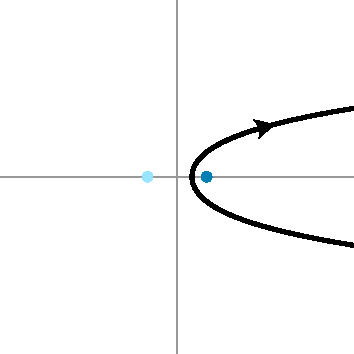
\includegraphics{figures/zeta_contour_3.pdf} \\[1em]
{\small The contour $\mathcal{H}^1_z$ in the $\zeta$ plane.}
\end{center}
From formula~15.4.14 in \cite{dlmf}, we learn that for our desired branch of $u$,
\[ \frac{1}{4u^2 - 1} = -F\big(\tfrac{1}{3}, \tfrac{2}{3}; \tfrac{1}{2}; \zeta^2\big), \]
so we can rewrite integral~\eqref{integral:mod-bessel-zeta} as
\[ K = \frac{1}{i\sqrt{3}} \int_{\mathcal{H}^1_z} e^{-z\zeta} F\big(\tfrac{1}{3}, \tfrac{2}{3}; \tfrac{1}{2}; \zeta^2\big)\;d\zeta. \]
This gives us an alternate route to the conclusion of Section~\ref{spatial}, which we'll follow below.

In addition to the solutions $v_1$ and $v_{-1}$ from Section~\ref{pos-root}\,--\, \ref{neg-root}, equation~\eqref{diff-eq:spatial-mod-bessel} has the solutions
\begin{alignat*}{2}
g_1 &\;=\;& & {}_2F_1\big(\tfrac{2}{3}, \tfrac{4}{3}; \tfrac{3}{2}; \xi_1\big) \\
g_{-1} &\;=\;&  & {}_2F_1\big(\tfrac{2}{3}, \tfrac{4}{3}; \tfrac{3}{2}; 1-\xi_1\big),
\end{alignat*}
given by formulas 15.10.11 and 15.10.13 from \cite{dlmf}.

The quadratic transformation identity 15.8.27 from \cite{dlmf} shows that\footnote{Note that $2\Gamma(\tfrac{1}{2})\Gamma(\tfrac{3}{2}) = 2\Gamma(\tfrac{1}{2})\,\tfrac{1}{2}\Gamma(\tfrac{1}{2}) = \pi$ and $\big[\Gamma(\tfrac{5}{6})\Gamma(\tfrac{7}{6})\big]^{-1} = \big[\Gamma(\tfrac{5}{6})\,\tfrac{1}{6}\Gamma(\tfrac{1}{6})\big]^{-1} = \frac{6\sin(\tfrac{1}{6} \pi)}{\pi} = \frac{3}{\pi}$.}
\[ F\big(\tfrac{1}{3}, \tfrac{2}{3}; \tfrac{1}{2}; \zeta^2\big) = \tfrac{1}{3}(g_1 + g_{-1}), \]
so we have
\[ K = \frac{1}{i\,3\sqrt{3}} \int_{\mathcal{H}^1_z} e^{-z\zeta} (g_1 + g_{-1})\;d\zeta. \]
The solution $g_{-1}$ is holomorphic on $\zeta \in [1, \infty)$, so it integrates to zero. The solution $g_1$, in contrast, is non-meromorphic at $\zeta = 1$. Along the branch cut $\zeta \in [1, \infty)$, its above-minus-below difference is $-\tfrac{3\sqrt{3}}{2}\,v_1$,
as given\footnote{Note that $\Gamma(\tfrac{3}{2}) \Gamma(\tfrac{1}{2})^{-1} = \tfrac{1}{2}$ and $\big[\Gamma(\tfrac{2}{3})\Gamma(\tfrac{4}{3})\big]^{-1} = \big[\Gamma(\tfrac{2}{3})\,\tfrac{1}{3}\Gamma(\tfrac{1}{3})\big]^{-1} = \frac{3\sin(\tfrac{1}{3} \pi)}{\pi} = \frac{3\sqrt{3}}{2\pi}$.} by equation~15.2.3 from \cite{dlmf}.
Hence,
\begin{align*}
K & = \frac{i}{2} \int^\infty_1 e^{-z\zeta} v_1\;d\zeta \\
e^z K & = \frac{i}{2} \int^\infty_1 e^{-z(\zeta - 1)} v_1\;d\zeta \\
e^z K & = \tfrac{i}{2} \laplace_{\zeta_1} v_1,
\end{align*}
just as we found in Section~\ref{bessel-regularity}. However, in this case, we get an exact equality (compared to the proportionality of Section~\ref{bessel-regularity}). 
\subsubsection{Another solution}
Section~\ref{contour-argument} associates the solution $K$ of equation~\eqref{eqn:mod-bessel} with the solution $g_1$ of equation~\eqref{diff-eq:hypergeom-pos}, which contributes the pole at $\zeta = 1$ of
\[ \frac{du}{d\zeta} = \frac{1}{4u^2 - 1} = \tfrac{1}{3}(g_1 + g_{-1}). \]
The solution $g_{-1}$, which contributes the pole at $\zeta = -1$, is associated with another solution of equation~\eqref{eqn:reg-mod-bessel}.
To express this other solution as a Laplace transform, following the method of Section~\ref{contour-argument}, we would use the solution
\[ v_{-1} = (1-\xi)^{-1/2} \,\, {}_2F_1\big(\tfrac{1}{6}, \tfrac{5}{6}; \tfrac{1}{2}; 1-\xi\big) \]
of equation~\eqref{diff-eq:spatial-mod-bessel}, given by formula~15.10.14 from \cite{dlmf}. This is the only solution, up to scale, which has a fractional power singularity at $\zeta = -1$.

In summary, the thimble projection technique of solving equation~\eqref{eqn:reg-mod-bessel} is associated with the basis
\begin{align*}
g_{1} & = {}_2F_1\big(\tfrac{2}{3}, \tfrac{4}{3}; \tfrac{3}{2}; \xi\big) \\
g_{-1} & = {}_2F_1\big(\tfrac{2}{3}, \tfrac{4}{3}; \tfrac{3}{2}; 1-\xi\big)
\end{align*}
of solutions for equation~\eqref{diff-eq:spatial-mod-bessel}, given by formulas 15.10.11 and 15.10.13 from \cite{dlmf}. These solutions contribute the poles at $\xi = 1$ and $\xi = 0$, respectively, of a generic solution.

The Laplace transformation method of solving equation~\eqref{eqn:reg-mod-bessel}, on the other hand, is associated with the basis
\begin{alignat*}{2}
v_{-1} &\;=\;& (1-\xi)^{-1/2} & \, {}_2F_1\big(\tfrac{1}{6}, \tfrac{5}{6}; \tfrac{1}{2}; 1-\xi\big) \\
v_1 &\;=\:& \xi^{-1/2} & \, {}_2F_1\big(\tfrac{1}{6}, \tfrac{5}{6}; \tfrac{1}{2}; \xi\big)
\end{alignat*}
given by formulas 15.10.14 and 15.10.12 from \cite{dlmf}. These solutions, up to scale, are the only ones with fractional power singularities.

Identities 15.10.18, and 15.10.22 from \cite{dlmf} give the change of basis
\begin{alignat*}{3}
v_{-1} &\;=\;&\tfrac{1}{\sqrt{3}}\,g_{-1} &\;+\;& \tfrac{1}{2}\,v_1 \\
v_1 &\;=\;& \tfrac{1}{\sqrt{3}}\,g_{1} &\;+\;& \tfrac{1}{2}\,v_{-1}.
\end{alignat*}
Summing these identities, we see that
\[ g_1 + g_{-1} = \tfrac{\sqrt{3}}{2}\,(f_1 + f_{-1}), \]
giving the alternate decomposition
\[ \frac{du}{d\zeta} = \tfrac{1}{2\sqrt{3}}\,(f_1 + f_{-1}). \]

\subsection{Thimble projection formula}

In the Airy-Lucas integral, $f$ is a Chebyshev polynomial, so we can do a thimble projection technique (see Section~\ref{contour-argument-AL}) or apply the thimble projection formula~\eqref{formula1} using trigonometric substitution. As an example of how one might reason in the latter case, we look at the Airy function, given by $f = 4u^3-3u$.

\textcolor{RoyalBlue}{[\ldots] this time applying the thimble projection formula to the generalized Cardano's formula.}

\textcolor{Peru}{Recall that the roots of $f(u)-\zeta$ can be written explicitly as 
\begin{align*}
    u(\zeta)&=\cos\Big(\frac{1}{3}\arccos\zeta-\frac{2\pi k}{3}\Big) \quad k=0,1,2\\
    &={}_2F_1\Big(-\frac{1}{6},\frac{1}{6};\frac{1}{2};1-\zeta^2\Big)
\end{align*}}
\textcolor{orange}{[Add the numerical check to show simple resurgence. For example, maybe graph exponential of the magnitude of function on position domain]}
The thimble $\Lambda_1$ can be parametrized by the path $\theta \mapsto \cosh(\theta - \tfrac{2}{3}\pi i)$. Since $4u^3 - 3u$ is the third Chebyshev polynomial and $\cosh$ is $2\pi$-periodic in the imaginary direction, the start and end points of $\Lambda_1(\zeta)$ are then characterized by
\begin{align*}
u & = \cosh(\mp\theta - \tfrac{2}{3}\pi i) \\
\zeta & = \cosh(3\theta).
\end{align*}
It follows that
\begin{align*}
\int_{\Lambda_1(\zeta)} \nu & = \int_{\Lambda_1(\zeta)} du \\
& = u \Big|_{\operatorname{start} \Lambda_1(\zeta)}^{\operatorname{end} \Lambda_1(\zeta)}\\
 & = \cosh(\theta - \tfrac{2}{3}\pi i) - \cosh(-\theta - \tfrac{2}{3}\pi i) \\
& = \big[\cosh(\theta) \cosh(-\tfrac{2}{3}\pi i) + \sinh(\theta) \sinh(-\tfrac{2}{3}\pi i)\big] \\
& \quad - \big[\cosh(-\theta) \cosh(-\tfrac{2}{3}\pi i) + \sinh(-\theta) \sinh(-\tfrac{2}{3}\pi i)\big] \\
& = 2\sinh(\theta) \sinh(-\tfrac{2}{3}\pi i) \\
& = -i\sqrt{3}\,\sinh(\theta).
\end{align*}
Let $\xi = \tfrac{1}{2}(1 - \zeta)$, and notice that $\xi = -\sinh\big(\tfrac{3}{2} \theta\big)^2$ at the start and end points. The identity~15.4.16 \cite{dlmf}
\[ \sinh( \theta) = \tfrac{1}{3} \sinh\big( \tfrac{3}{2}\theta\big)\,{}_2F_1\big(\tfrac{1}{6}, \tfrac{5}{6}; \tfrac{3}{2}; -\sinh\big(\tfrac{3}{2}\theta\big)^2\big) \]
then shows us that
\[ \frac{i}{\sqrt{3}} \int_{\Lambda_1(\zeta)} \nu = (-\xi)^{1/2}\,{}_2F_1\big(\tfrac{1}{6}, \tfrac{5}{6}; \tfrac{3}{2}; \xi\big). \]

Now we can evaluate the half-integral of $\int_{\Lambda_1} \nu$ using Bateman's fractional integral formula for hypergeometric functions see \cite[Section 4.1]{koornwinder2015fractional}.
\begin{align*}
\fracderiv{-1/2}{\zeta}{1} \left( \int_{\Lambda_1(\zeta)} \nu \right) & = \frac{1}{\Gamma\big(\tfrac{1}{2}\big)} \int_{1}^\zeta (\zeta - \zeta')^{-1/2} \left( \int_{\Lambda_1(\zeta')} \nu \right)\,d\zeta' \\
& = \frac{1}{\Gamma\big(\tfrac{1}{2}\big)} \int_0^\xi  (\xi' - \xi)^{-1/2} \Big[ -{i}{\sqrt{3}}\, (-\xi)^{1/2}\,{}_2F_1\big(\tfrac{1}{6}, \tfrac{5}{6}; \tfrac{3}{2}; \xi\big) \Big] \,\big( -\,d\xi' \big) \\
& = -i \frac{\Gamma\big(\tfrac{3}{2}\big)}{\Gamma(2)} (-\xi)\,{}_2F_1\big(\tfrac{1}{6}, \tfrac{5}{6}; 2; \xi\big) \\
& = \frac{i}{2} \sqrt{\pi}\,\xi\, {}_2F_1\big(\tfrac{1}{6}, \tfrac{5}{6}; 2; \xi\big).
\end{align*}
Finally, we differentiate twice using 15.5.4 and 15.5.1 from \cite{dlmf}.
\begin{align*}
\fracderiv{3/2}{\zeta}{1} \left( \int_{\Lambda_1(\zeta)} \nu \right) & = \left(-\tfrac{\partial}{\partial \xi}\right)^2 \left[ \frac{i\sqrt{\pi}}{2}\,\xi\, {}_2F_1\big(\tfrac{1}{6}, \tfrac{5}{6}; 2; \xi\big) \right] \\
& =  \tfrac{i\sqrt{\pi}}{2} \left(\tfrac{\partial}{\partial \xi}\right)^2 \left[ \xi\,{}_2F_1\big(\tfrac{1}{6}, \tfrac{5}{6}; 2; \xi\big) \right] \\
& = \tfrac{i\sqrt{\pi}}{2}\,\tfrac{\partial}{\partial \xi} \left[ {}_2F_1\big(\tfrac{1}{6}, \tfrac{5}{6}; 1; \xi\big) \right] \\
& = \tfrac{i\sqrt{\pi}}{2}\,\tfrac{5}{12}\, {}_2F_1\big(\tfrac{7}{6}, \tfrac{11}{6}; 2; \xi\big).
\end{align*}
%
For completeness, we repeat the computations for $\hat{\phi}_{-1}$: the thimble $\Lambda_{-1}$ can be parametrized by the path $\theta \mapsto -\cosh(\theta - \tfrac{2}{3}\pi i)$. Hence,
\begin{align*}
\int_{\Lambda_{-1}(\zeta)} \nu & = \int_{\Lambda_{-1}(\zeta)} du \\
& = u \Big|_{\operatorname{start} \Lambda_{-1}(\zeta)}^{\operatorname{end}\Lambda_{-1}(\zeta)}.
\end{align*}
The start and end points of $\Lambda_{-1}$ are characterized by
\begin{align*}
u & = -\cosh(\mp\theta - \tfrac{2}{3}\pi i) \\
\zeta & = -\tfrac{2}{3} \cosh(3\theta),
\end{align*}
so
\begin{align*}
\int_{\Lambda_{-1}(\zeta)} \nu & =- \cosh(\theta - \tfrac{2}{3}\pi i) + \cosh(-\theta - \tfrac{2}{3}\pi i) \\
& =- \big[\cosh(\theta) \cosh(-\tfrac{2}{3}\pi i) + \sinh(\theta) \sinh(-\tfrac{2}{3}\pi i)\big] \\
& \quad + \big[\cosh(-\theta) \cosh(-\tfrac{2}{3}\pi i) + \sinh(-\theta) \sinh(-\tfrac{2}{3}\pi i)\big] \\
& = 2\sinh(\theta) \sinh(\tfrac{2}{3}\pi i) \\
& = i\sqrt{3}\,\sinh(\theta)
\end{align*}
Let $\xi = \tfrac{1}{2}(1 + \zeta)$, and notice that $\xi =- \sinh( \theta)^2$ at the start and end points. The identity~15.4.16 in \cite{dlmf}
\[ \sinh(\theta) = \sinh(\theta)\, {}_2F_1\big(\tfrac{1}{6}, \tfrac{5}{6}; \tfrac{3}{2}; -\sinh(\theta)^2\big) \]
then shows us that
\[ -\frac{i}{\sqrt{3}} \int_{\mathcal{C}_-(\zeta)} \nu =  (-\xi)^{1/2}\, {}_2F_1\big(\tfrac{1}{6}, \tfrac{5}{6}; \tfrac{3}{2}; \xi\big). \]

Now we can evaluate the half-integral of $\int_{\Lambda_{-1}} \nu$ using Bateman's fractional integral formula for hypergeometric functions: \begin{align*}
\fracderiv{-1/2}{\zeta}{-1}\left( \int_{\Lambda_{-1}(\zeta)} \nu \right) & = \frac{1}{\Gamma\big(\tfrac{1}{2}\big)} \int_{-1}^\zeta (\zeta - \zeta')^{-1/2} \left( \int_{\Lambda_{-1}(\zeta')} \nu \right)\,d\zeta' \\
& = \frac{1}{\Gamma\big(\tfrac{1}{2}\big)} \int_0^\xi  (\xi - \xi')^{-1/2} \Big[{i}{\sqrt{3}}\, (-\xi')^{1/2}\, {}_2F_1\big(\tfrac{1}{6}, \tfrac{5}{6}; \tfrac{3}{2}; \xi' \big) \Big] \,\big( \,d\xi' \big) \\
& =  \frac{\Gamma\big(\tfrac{3}{2}\big)}{\Gamma(2)} (-\xi)\, {}_2F_1\big(\tfrac{1}{6}, \tfrac{5}{6}; 2; \xi\big) \\
& = - \tfrac{\sqrt{\pi}}{2}\,\xi\,{}_2F_1\big(\tfrac{1}{6}, \tfrac{5}{6}; 2; \xi\big).
\end{align*}
Finally, we differentiate twice using 15.5.4 and 15.5.1 from \cite{dlmf}
\begin{align*}
\fracderiv{3/2}{\zeta}{-1} \left( \int_{\Lambda_{-1}(\zeta)} \nu \right) & = \left(\tfrac{\partial}{\partial \xi}\right)^2 \left[ - \tfrac{\sqrt{\pi}}{2} \,\xi\, {}_2F_1\big(\tfrac{1}{6}, \tfrac{5}{6}; 2; \xi\big) \right] \\
& = - \tfrac{\sqrt{\pi}}{2} \left(\tfrac{\partial}{\partial \xi}\right)^2 \left[ \xi\, {}_2F_1\big(\tfrac{1}{6}, \tfrac{5}{6}; 2; \xi\big) \right] \\
& = - \tfrac{\sqrt{\pi}}{2}\,\tfrac{\partial}{\partial \xi} \left[ {}_2F_1\big(\tfrac{1}{6}, \tfrac{5}{6}; 1; \xi\big) \right] \\
& = - \tfrac{\sqrt{\pi}}{2}\,\tfrac{5}{12}\, {}_2F_1\big(\tfrac{7}{6}, \tfrac{11}{6}; 2; \xi\big).
\end{align*}
\subsubsection{An eye on resurgence}\label{apx:eye-res-airy}
\textcolor{orange}{[Add link to general references in intro].} Resurgent functions in the position domain are characterized by being ``endlessly analytically continuable'' away from their singularities~\textcolor{magenta}{\cite[Section~1.2.2]{intro-to-ecalle}\{this paper only defines resurgent functions in the frequency domain\}\{For definition in the position domain, cite \S 6.1 of Mitschi and Sauzin~\cite{diverg-resurg-i}\}}. \textcolor{MediumSeaGreen}{[Focus on endlessly continuable functions instead? See~[Section~2, ``Variations on the resurgence of the gamma function''.]} \textcolor{red}{They have the special property that by studying their analytic continuation around one singularity, we can typically discover the germ of another singularity.} \textcolor{RoyalBlue}{They have the very special property that by studying one germ, we can typically reconstruct the others by looking at the behavior near the singular points.} \textcolor{MediumSeaGreen}{[They are ``self-reproducing'' in a certain remarkable way involving holonomy around singularities, as we'll see in the example below\ldots]} A prototypical class of resurgent functions is the so-called simple resurgent functions~\textcolor{magenta}{\cite[Section~1.2.3]{intro-to-ecalle}\{oops, this source defines simple resurgent functions in the frequency domain\}}.  namely an \textcolor{Maroon}{[resurgent]} analytic function $\hat{\phi}$ in the position domain with singularities $\omega$ such that

\textcolor{Maroon}{[\ldots] resurgent function with the property that at each singularity $\omega$, we have an expansion of the form}
\begin{align*}
    \hat{\phi} = \frac{C_\omega}{\zeta_\omega}+\frac{S_\omega}{2\pi i} \log(\zeta_\omega)\,\series{\phi}_\omega + \text{ hol. funct.} \textcolor{Maroon}{[\text{convergent series in}\,\zeta_\omega]}
\end{align*}
where \textcolor{Maroon}{$\zeta = \omega + \zeta_\omega$, $\series{\phi}_\omega$ is a series in $\zeta_\omega$} $C_\omega, S_\omega$ are constants and $S_\omega$ is typically assumed to be integral (in a suitable normalization) and called the Stokes constant of the singularity $\omega$. The goal of resurgence is to investigate the location of the singularities together with their Stokes constants and the corresponding germs $\series{\phi}_\omega$.  
%The main idea of resurgence is that studying the analytic continuation of $\tilde{\phi}_\omega$  

Thimbles integrals are good candidates to understand the structure of resurgent functions; indeed the functions $\hat{\phi}_j$ in equation \eqref{formula1} are resurgent. Their resurgent structure can be easily reconstructed: if $\nu$ is holomorphic, then $\hat{\phi}_j$ is singular at $\zeta_j=\alpha_k$ for $k\neq j$. Hence the set of singularities is given by the critical values of $f$. Then, the computation of the Stokes constants and of the other germs $\series{\phi}_k$ is done by studying $\hat{\phi}_j$ near its singular points. For example, for the Airy function, we can expand $\hat{\phi}_1$ near $\zeta=-1$:
\begin{align*}
    \hat{\phi}_1(\zeta-1)=\frac{36}{5\pi}\frac{1}{\zeta}+\frac{1}{2\pi}\log(\zeta) \left(1+\frac{77}{144}\zeta+\frac{17017}{62208}\zeta^2+\frac{7436429}{53747712}\zeta^3+\ldots\right)  +\text{ hol. funct. }
\end{align*}

Notice that $(1+\tfrac{77}{144}\zeta+\tfrac{17017}{62208}\zeta^2+\tfrac{7436429}{53747712}\zeta^3+\ldots)$ is the Taylor series of $\hat{\phi}_{-1}$ at the origin. So we see that expanding $\hat{\phi}_1$ at the singularity we see the germ of another singularity $\series{\phi}_{-1}$. Analogously, if we expand $\hat{\phi}_{-1}$ near $\zeta=1$ we find
\begin{align*}
    \hat{\phi}_{-1}(\zeta+1)=-\frac{36}{5\pi}\frac{1}{\zeta}+\frac{1}{2\pi}\log(\zeta) \left(1-\frac{77}{144}\zeta+\frac{17017}{62208}\zeta^2-\frac{7436429}{53747712}\zeta^3+\ldots\right) +\text{ hol. funct. }
\end{align*}
where the germ $(1-\tfrac{77}{144}\zeta+\tfrac{17017}{62208}\zeta^2-\tfrac{7436429}{53747712}\zeta^3+\ldots)$ is the Taylor expansion of $\hat{\phi}_1$ at the origin. 
From these expressions, we also noticed that $\hat{\phi}_i$ are simple resurgent functions.   

\subsection{Comparison with other treatments of the Airy equation}

\subsubsection{Different Borel transform convention} Physicists often use a different version of the Borel transform:
\begin{align*}
\borel_{\textit{phys}} \maps \C \llbracket z^{-1} \rrbracket & \to \C \llbracket \zeta \rrbracket \\
z^{-n} & \mapsto \frac{\zeta^n}{n!}.
\end{align*}
This version avoids sending $1$ to the convolution unit $\delta$, at the cost of no longer mapping multiplication to convolution or inverting the formal Laplace transform. It's sometimes convenient to $\borel_\textit{phys}(f) = \borel(z^{-1} f)$.

For problems involving a small parameter $\hbar$ rather than a large parameter $z$, physicists also define
\begin{align*}
\borel_{\textit{phys}} \maps \C \llbracket \hbar \rrbracket & \to \C \llbracket \zeta \rrbracket \\
\hbar^n & \mapsto \frac{\zeta^n}{n!}.
\end{align*}
From a combinatorial perspective, this is just the transformation that sends an ordinary generating function to the corresponding exponential generating function.

In \cite{lectures-Marino}, the author studies the Airy functions as an example of resurgent functions. He starts with the formal trans-monomial solutions of the Airy equation:

\begin{align*}
\tilde{\Phi}_{\mathrm{Ai}}(x)&=\frac{1}{2\sqrt{\pi}}x^{-1/4}e^{-\tfrac{2}{3}x^{3/2}}\tilde{W}_1(x^{-3/2})\\
\tilde{\Phi}_{\mathrm{Bi}}(x)&=\frac{1}{2\sqrt{\pi}}x^{-1/4}e^{\tfrac{2}{3}x^{3/2}}\tilde{W}_2(x^{-3/2})
\end{align*}  
where 
\begin{align*}
\tilde{W}_{1,2}(\hbar)=\sum_{n=0}^{\infty}\frac{1}{2\pi}\left(\mp\frac{3}{4}\right)^{n}\frac{\Gamma(n+\frac{5}{6})\Gamma(n+\frac{1}{6})}{n!}\hbar^n.
\end{align*}
%Notice that $\tilde{W}_{1,2}(\hbar)$ are proportional to $\tilde{W}_{\pm}(z)$ with $z=\hbar^{-1}$. However, their Borel transforms are two different hypergeometric functions:
Then, by applying the two definitions of the Borel transform $\borel_{\textit{phys}}$ and $\borel$, on the one hand we have  
\begin{align*}
w_{1,2}(\zeta)&\defeq\borel_{\textit{phys}}(\tilde{W}_{1,2})(\zeta)\\
&=\sum_{n=0}^{\infty}\frac{1}{2\pi}\left(\mp\frac{3}{4}\right)^{n}\frac{\Gamma(n+\frac{5}{6})\Gamma(n+\frac{1}{6})}{n!}\frac{\zeta^n}{n!}\\
&={}_2F_1\left(\frac{1}{6},\frac{5}{6};1;\mp\frac{3}{4}\zeta\right) 
\end{align*}
on the other hand, we find
\begin{align*}
\borel(\tilde{W}_{1,2})(\zeta)&=\frac{1}{2\pi}\delta+\sum_{n=1}^{\infty} \frac{1}{2\pi}\left(\mp\frac{3}{4}\right)^{n}\frac{\Gamma(n+\frac{5}{6})\Gamma(n+\frac{1}{6})}{n!}\frac{\zeta^{n-1}}{(n-1)!}\\
&=\frac{1}{2\pi}\delta+\sum_{n=0}^{\infty} \frac{1}{2\pi}\left(\mp\frac{3}{4}\right)^{n+1}\frac{\Gamma(n+1+\frac{5}{6})\Gamma(n+1+\frac{1}{6})}{(n+1)!}\frac{\zeta^{n}}{n!}\\
&=\frac{1}{2\pi}\delta\mp\frac{3}{4}\sum_{n=0}^{\infty} \frac{1}{2\pi}\left(\mp\frac{3}{4}\right)^{n}\frac{\Gamma(n+\frac{11}{6})\Gamma(n+\frac{7}{6})}{\Gamma(n+2)}\frac{\zeta^{n}}{n!}\\
&=\frac{1}{2\pi}\delta\mp\frac{5}{48} {}_2F_1\left(\frac{7}{6},\frac{11}{6};2;\mp\frac{3}{4}\zeta\right)%\\
%&=\frac{1}{2\pi}\delta\mp \frac{5}{48}\frac{1}{c_{1,2}}w_{\pm}(\zeta)
%w_{\pm}(\zeta)&=c_{1,2}\,\,{}_2F_1\left(\frac{7}{6},\frac{11}{6};2;\mp\frac{3}{4}\zeta\right) &\qquad \text{see \eqref{eq:hat+}\eqref{eq:hat-}}
\end{align*}
%That ambiguity comes from the different definitions of Borel transforms: 
%\begin{align*}
%\borel(\tilde{W}_{1,2})(\zeta)&=\frac{1}{2\pi}\delta+\sum_{n=1}^{\infty} \frac{1}{2\pi}\left(\mp\frac{3}{4}\right)^{n}\frac{\Gamma(n+\frac{5}{6})\Gamma(n+\frac{1}{6})}{n!}\frac{\zeta^{n-1}}{(n-1)!}\\
%&=\frac{1}{2\pi}\delta+\sum_{n=0}^{\infty} \frac{1}{2\pi}\left(\mp\frac{3}{4}\right)^{n+1}\frac{\Gamma(n+1+\frac{5}{6})\Gamma(n+1+\frac{1}{6})}{(n+1)!}\frac{\zeta^{n}}{n!}\\
%&=\frac{1}{2\pi}\delta\mp\frac{3}{4}\sum_{n=0}^{\infty} \frac{1}{2\pi}\left(\mp\frac{3}{4}\right)^{n}\frac{\Gamma(n+\frac{11}{6})\Gamma(n+\frac{7}{6})}{\Gamma(n+2)}\frac{\zeta^{n}}{n!}\\
%&=\frac{1}{2\pi}\delta\mp\frac{5}{48} {}_2F_1\left(\frac{7}{6},\frac{11}{6};2;\mp\frac{3}{4}\zeta\right)%\\
%%&=\frac{1}{2\pi}\delta\mp \frac{5}{48}\frac{1}{c_{1,2}}w_{\pm}(\zeta)
%\end{align*}  

and comparing the two solutions we notice that up to the factor of $\delta$

\begin{equation}\label{Borel-W12}
\borel(\tilde{W}_{1,2})(\zeta)-\frac{1}{2\pi}\delta=\mp \frac{5}{48} {}_2F_1\left(\frac{7}{6},\frac{11}{6};2;\mp\frac{3}{4}\zeta\right)=\frac{d}{d\zeta}\borel_{\textit{phys}}(\tilde{W}_{1,2})(\zeta) 
\end{equation}
More generally, if $\tilde{\Phi}(z)\in z^{-1}\C \llbracket z^{-1} \rrbracket$, i.e. it has no constant term, then 

\begin{equation}
\frac{d}{d\zeta}\circ\borel_{\textit{phys}}\tilde{\Phi}=\borel\tilde{\Phi}.
\end{equation}
In particular, $\frac{d}{d\zeta}\circ\borel_{\textit{phys}}\left[z^{-1/2}\tilde{W}_{1}\right]\left(\frac{2}{3}\zeta\right)=v_1(\zeta)$. 

%Recall that $v_1$ (computed in Section~\ref{pos-root}) is proportional to the Borel transform of $ z^{-1/2}\tilde{W}_1(z)$ (see Section~\ref{bessel-regularity}). We want to compare $v_1$ with the \textit{physic} Borel transform $\borel_{\textit{phys}}$ of $z^{-1/2}\tilde{W}_1$:
%
%\begin{align*}
%\borel_{\textit{phys}}(z^{-1/2}\tilde{W}_{1})\left(\frac{2}{3}\zeta\right)&=\sum_{n=0}^{\infty}\frac{1}{2\pi}\left(-\frac{1}{2}\right)^{n}\frac{\Gamma(n+\frac{5}{6})\Gamma(n+\frac{1}{6})}{n!}\frac{\zeta^{n+\frac{1}{2}}}{\Gamma(n+3/2)}\\
%&=\frac{1}{2\pi}\zeta^{-1/2}\sum_{n=0}^{\infty}\frac{\Gamma(n+\frac{5}{6})\Gamma(n+\frac{1}{6})}{n!\Gamma(n+3/2)}\left(-\frac{\zeta}{2}\right)^{n+1}\\
%&=\frac{1}{2\pi}\zeta^{1/2}\,\, {}_2F_1\left(\frac{1}{6},\frac{5}{6};\frac{3}{2};-\frac{\zeta}{2}\right) 
%\end{align*}
%
%Now taking the $-1$- derivative of $v_1(\zeta)$ we get
%
%\begin{align*}
%\partial_\zeta^{-1} v_1&=\frac{1}{\Gamma(1)}\int_0^{\zeta}(\zeta-\zeta') v_1(\zeta')d\zeta'\\
%&=\int_0^{\zeta}(\zeta-\zeta') \zeta'^{-1/2} \,\, {}_2F_1\left(\frac{1}{6},\frac{5}{6};\frac{1}{2};-\frac{\zeta'}{2}\right)d\zeta'\\
%&=\frac{\Gamma(1/2)}{\Gamma(3/2)}\zeta^{1/2} \,\, {}_2F_1\left(\frac{1}{6},\frac{5}{6};\frac{3}{2};-\frac{\zeta}{2}\right)\\
%&=2 \zeta^{1/2} \,\, {}_2F_1\left(\frac{1}{6},\frac{5}{6};\frac{3}{2};-\frac{\zeta}{2}\right)
%\end{align*}



\subsubsection{Integral formula for hypergeometric functions}

In \cite{diverg-resurg-i} the author studies summability and resurgent properties of solutions of the Airy equation. 

He considers the formal power series  
\[\tilde{\Phi}_{\pm}(z)\defeq \sum_{n=0}^{\infty}\frac{1}{2\pi}\left(\mp\frac{1}{2}\right)^{n}\frac{\Gamma(n+\frac{5}{6})\Gamma(n+\frac{1}{6})}{n!}z^{-n}\]
such that
\begin{align*}
\tilde{\Phi}_{\mathrm{Ai}}(y)&=\frac{1}{2\sqrt{\pi}}y^{-1/4}e^{-\tfrac{2}{3}y^{3/2}}\tilde{\Phi}_{+}\left(\tfrac{2}{3}y^{3/2}\right)\\
\tilde{\Phi}_{\mathrm{Bi}}(y)&=\frac{1}{2\sqrt{\pi}}y^{-1/4}e^{\tfrac{2}{3}y^{3/2}}\tilde{\Phi}_{-}\left(\tfrac{2}{3}y^{3/2}\right)
\end{align*} 
are formal solutions of the Airy equation. Notice that compared to Marino's formal solutions, Sauzin adopts a different change of coordinates $z=\frac{2}{3}y^{3/2}$.  

By looking for solutions of the Borel transformed equation, he wrote the Borel transform of $\tilde{\Phi}_{\pm}$ as a convolution product: 

\begin{align*}
\hat{\phi}_+(\zeta):=\borel\tilde{\Phi}_+=\delta+\frac{d}{d\zeta}\hat{\chi}(\zeta)  \qquad \hat{\phi}_-(\zeta):=\borel\tilde{\Phi}_-=\delta-\frac{d}{d\zeta}\hat{\chi}(-\zeta)
\end{align*}
 where $\hat{\chi}(\zeta)=\frac{2^{1/6}}{\Gamma(1/6)\Gamma(5/6)}(2\zeta+\zeta^2)^{-1/6}\ast \zeta^{-5/6}$.

%Notice that $\tilde{W}_{1,2}(\tfrac{2}{3}\hbar)=\tilde{\Phi}_{\pm}(z)$ for $\hbar=z^{-1}$, hence 
%
%\begin{align*}
%\tilde{\phi}_{+}(\zeta)&=\borel\tilde{W}_{1}(\tfrac{2}{3}\zeta)=\frac{1}{2\pi}\delta-\frac{5}{48} {}_2F_1\left(\frac{7}{6},\frac{11}{6};2;-\frac{\zeta}{2}\right) \\
%\tilde{\phi}_{-}(\zeta)&=\borel\tilde{W}_{2}(\tfrac{2}{3}\zeta)=\frac{1}{2\pi}\delta+\frac{5}{48} {}_2F_1\left(\frac{7}{6},\frac{11}{6};2;\frac{\zeta}{2}\right) 
%\end{align*}
%which up to a constant factor for $\delta$, they agree with our results. 

Notice that the function $\hat{\chi}(\zeta)$ is an hypergeometric function:

\begin{align*}
\hat{\chi}(\zeta)&=\frac{2^{1/6}}{\Gamma(1/6)\Gamma(5/6)}(2\zeta+\zeta^2)^{-1/6}\ast \zeta^{-5/6}\\
&=\frac{2^{1/6}}{\Gamma(1/6)\Gamma(5/6)}\int_0^{\zeta}(2\zeta'+\zeta'^2)^{-1/6} (\zeta-\zeta')^{-5/6}d\zeta'\\
&=\frac{2^{1/6}}{\Gamma(1/6)\Gamma(5/6)}\int_0^{1}(\zeta t)^{-1/6}(2+\zeta t)^{-1/6} (\zeta-\zeta t)^{-5/6} \zeta dt\\
&=\frac{2^{1/6}}{\Gamma(1/6)\Gamma(5/6)}\int_0^{1} t^{-1/6} 2^{-1/6}(1+\frac{\zeta}{2} t)^{-1/6} (1-t)^{-5/6}d\zeta'\\
&=\frac{1}{\Gamma(1/6)\Gamma(5/6)}\int_0^{1} t^{-1/6} (1+\frac{\zeta}{2} t)^{-1/6} (1-t)^{-5/6}d\zeta'\\
&={}_2F_1\left(\frac{1}{6},\frac{5}{6};1;-\frac{\zeta}{2}\right)
\end{align*}
where in the last step we use the Euler formula for hypergeometric functions \footnote{The Euler formula is \begin{equation}\label{Euler formula}
{}_{2}F_1\left(a,b;c;x\right)=\frac{\Gamma(c)}{\Gamma(b)\Gamma(c-b)}\int_0^1 t^{b-1}(1-t)^{c-b-1}(1-xt)^{-a}dt.
\end{equation}}. Then, by taking derivatives we recover $\hat{\phi}_{\pm}(\zeta)$: 

\begin{align*}
\hat{\phi}_+(\zeta)&=\delta-\frac{1}{2}\frac{5}{36}\,\, {}_2F_1\left(\frac{7}{6},\frac{11}{6};2;-\frac{\zeta}{2}\right)=\delta-\frac{2}{3}\frac{5}{48} {}_2F_1\left(\frac{7}{6},\frac{11}{6};2;-\frac{\zeta}{2}\right)\\
\hat{\phi}_-(\zeta)&=\delta+\frac{1}{2}\frac{5}{36}\,\, {}_2F_1\left(\frac{7}{6},\frac{11}{6};2;\frac{\zeta}{2}\right)=\delta+\frac{2}{3}\frac{5}{48} {}_2F_1\left(\frac{7}{6},\frac{11}{6};2;\frac{\zeta}{2}\right)
\end{align*} 
and up to a multiplicative constant they match our computations for $\borel(\tilde{W}_{1,2})$ (see equation~\eqref{Borel-W12}).
The main advantage of writing Gauss hypergeometric functions as a convolution product relies on \'Ecalle's singularity theory. Indeed $(2\zeta+\zeta^2)^{-1/6}$ extends analytically to the universal cover of $\C\setminus\lbrace 0,-2\rbrace$ and the convolution with $\zeta^{-5/6}$ does not change the set of singularities (see part c of \cite[Section 6.14.5]{diverg-resurg-i}). Furthermore, the author proves that $\hat{\phi}_{\pm}(\zeta)$ are simple resurgent functions (see \cite[Lemma 6.106]{diverg-resurg-i}). %Therefore, from the expression of $\chi(\zeta)$ as a convolution product, the resurgent properties of $\tilde{\phi}_{\pm}(\zeta)$ are evident.  

\subsubsection{Comparison with exact WKB}

Kawai and Takei study the WKB analysis of the Airy--type Schrodinger equation

\begin{equation}
\label{WKB_Airy} 
\left[\left(\frac{d}{dx}\right)^2 - \eta^2 x \right] \psi(x, \eta) = 0 
\end{equation}
as $\eta\to\infty$. They define $\psi_B(x, y)$ as the inverse Laplace transform of $\psi(x, \eta)$ with respect to $\eta$. In the coordinate $t=\frac{3}{2}yx^{-3/2}$ they find an explicit formula for $\psi_B(x,y)$ in terms of Gauss hypergeometric functions:
\begin{align*}
\psi_{+,B}(x,y)&=\frac{1}{x}\phi_+(t)=\frac{\sqrt{3}}{2\sqrt{\pi}}\frac{1}{x}s^{-1/2}\, {}_2F_1\left(\frac{1}{6},\frac{5}{6};\frac{1}{2};s\right)\\
\psi_{-,B}(x,y)&=\frac{1}{x}\phi_-(t)=\frac{\sqrt{3}}{2\sqrt{\pi}}\frac{1}{x}(1-s)^{-1/2}\, {}_2F_1\left(\frac{1}{6},\frac{5}{6};\frac{1}{2};1-s\right)
\end{align*}
where $s=t/2+1/2$. 
The same hypergeometric functions have been computed in Section \ref{Airy} as the Borel transform of the formal solutions of the Airy equation

\begin{equation}
\label{Airy}
\left[\left(\frac{d}{dw}\right)^2 -  w \right] f(w) = 0.
\end{equation}

Although the two equations look closely related (they are equivalent by the change of coordinates $w=x\eta^{2/3}$), the Borel transform of $\psi$ is computed with respect to $\frac{2}{3}\eta x^{3/2}$ (which is the conjugate variable of $t$) while the Borel transform of $f(w)$ is computed with respect to $w$. So we need to find a different change of coordinates to explain why the Borel transforms of $\psi(x,\eta)$ and $f(w)$ are given by the same hypergeometric function. 

First of all notice that if $\eta$ and $y$ are conjugate variables under Borel transform, meaning 
\begin{align*}
\sum_{n\geq 0}a_n\eta^{-n-1}  \overset{\borel}{\longrightarrow} \sum_{n\geq 0}\frac{a_n}{n!} y^{n} 
\end{align*} 
then $t=\frac{3}{2}yx^{-3/2}$ is the conjugate variable of $q=\frac{2}{3}\eta x^{3/2}$ up to correction by a factor of $\frac{3}{2}x^{-3/2}$
\begin{align*}
\sum_{n\geq 0}a_nq^{-n-1}=\sum_{n\geq 0}a_nx^{-3/2(n+1)}\left(\frac{2}{3}\eta\right)^{-n-1}  \overset{\borel}{\longrightarrow} \sum_{n\geq 0}\frac{a_nx^{-3/2(n+1)}}{n!}\left(\frac{3}{2}\right)^{n+1}  y^{n}=\frac{3}{2}x^{-3/2}\sum_{n\geq 0}\frac{a_n}{n!} t^{n}. 
\end{align*}
In addition, $\psi_{B,\pm}(x,y)=\frac{1}{x}\phi_{\pm}(t)$, therefore we expect that $\psi(x,\eta)=x^{1/2}\Phi(q)$. Assume that $\psi(x,y)$ is a solution of \eqref{WKB_Airy}, then $\Phi(q)$ solves 
\begin{equation}
\label{eq_Phi}
\left[\left(\frac{d}{dx}\right)^2+x^{-1}\frac{d}{dx}-\frac{1}{4}x^{-2} - \eta^2 x \right] \Phi(q) = 0
\end{equation}

\begin{proof}
\begin{align*}
&\left[\left(\frac{d}{dx}\right)^2 - \eta^2 x \right] \psi(x, \eta) = 0\\
&\left[\left(\frac{d}{dx}\right)^2 - \eta^2 x \right] x^{1/2}\Phi(q) = 0\\
&\frac{d}{dx}\left[\frac{1}{2}x^{-1/2}\Phi+x^{1/2}\frac{d}{dx}\Phi\right]-\eta^2x^{3/2}\Phi=0\\
&-\frac{1}{4}x^{-3/2}\Phi+\frac{1}{2}x^{-1/2}\frac{d}{dx}\Phi+\frac{1}{2}x^{-1/2}\frac{d}{dx}\Phi+x^{1/2}\left(\frac{d}{dx}\right)^2\Phi-\eta^2x^{3/2}\Phi=0\\
&\left[x^{1/2}\left(\frac{d}{dx}\right)^2+x^{-1/2}\frac{d}{dx}-\frac{1}{4}x^{-3/2}-\eta^2x^{3/2}\right]\Phi=0\\
&\left[\left(\frac{d}{dx}\right)^2+x^{-1}\frac{d}{dx}-\frac{1}{4}x^{-2}-\eta^2x\right]\Phi=0
\end{align*}
\end{proof}
Now rewrite \eqref{eq_Phi} in the coordinates $q=\frac{2}{3}\eta x^{3/2}$: 
\begin{align*}
&\left[\left(\frac{d}{dx}\right)^2+x^{-1}\frac{d}{dx}-\frac{1}{4}x^{-2}-\eta^2x\right]\Phi=0\\
&\left[\eta^2x\left(\frac{d}{dq}\right)^2+\frac{1}{2}\eta x^{-1/2}\frac{d}{dq}+x^{-1}\cdot\, \eta\,  x^{1/2}\frac{d}{dq}-\frac{1}{4}x^{-2}-\eta^2x\right]\Phi=0\\
&\left[\eta^2x\left(\frac{d}{dq}\right)^2+\frac{3}{2}\eta x^{-1/2}\frac{d}{dq}-\frac{1}{4}x^{-2}-\eta^2x\right]\Phi=0\\
&\left[\left(\frac{d}{dq}\right)^2+\frac{3}{2}\eta^{-1} x^{-3/2}\frac{d}{dq}-\frac{1}{4}\eta^{-2}x^{-3}-1\right]\Phi=0\\
%&\left[\left(\frac{d}{dq}\right)^2+\eta^{-1} x^{-3/2}\frac{d}{dq}-\frac{1}{9}\eta^{-2}x^{-3}-1\right]\Phi=0\\
&\left[\left(\frac{d}{dq}\right)^2+q^{-1}\frac{d}{dq}-\frac{1}{9}q^{-2}-1\right]\Phi=0
\end{align*}

therefore $\Phi(q)$ is a solution of the transformed Airy equation \eqref{eqn:reg-mod-bessel}. 

\begin{remark}
The change of coordinate $q=\frac{2}{3}\eta x^{3/2}$ is not casual: recall that the WKB ansatz for a Schrodinger type equation is

\begin{equation}
\psi(x,\eta)=\exp\left(\int_{x_0}^xS(\eta,x')dx'\right)
\end{equation} 
 and $S(\eta,x)=\sum_{k\geq -1}S_k(x)\eta^{-k}$. In addition, for the Airy--type Schrodinger equation 
 \begin{align*}
 S_{-1}^2=x
 \end{align*}
hence, up to a choice of sign for the square root
\begin{align*}
q&=\frac{2}{3}\eta x^{3/2}=\eta\int_0^x\sqrt{x'}dx'=\eta\int_{0}^xS_{-1}(x')dx'.
\end{align*}
We expect that the change of coordinates $q=\eta\int_0^{x}S_{-1}(x')dx'$ would explain the analogies between the Borel transform of the WKB solution of a Schrodinger equation and the Borel transform of the associated ODE.  
\end{remark} 

\section{Facts about differential and integral equations}
%%\section{Generalities about ODEs and Integral Equations}\label{apx:generalities_ODEs}
\textcolor{red}{Shall we review the content of \cite{reg-sing-volterra}?}
\subsection{Passing between the analytic world and the formal world}
\textcolor{orange}{Show that the Taylor expansion of an analytic solution of an integral equation satisfies the same equation (or just cite the statement in Erdelyi). Cite the theorem of Erdelyi which shows that a solution of a differential equation (under certain conditions) has an asymptotic expansion, which satisfies the corresponding differential equation.}
\subsection{Order shifting}\label{shifting}
Consider holomorphic functions on a simply connected open domain $\Omega$ that touches but doesn't contain $\zeta = 0$. %A function is {\em regular} at $\zeta = 0$ if it extends holomorphically over that point. %We'll say a function is {\em slight} at $\zeta = 0$ if it can be written as 
%\begin{equation}\label{eqn:slight-defn}
%\zeta^{\alpha_1} f_1 + \ldots + \zeta^{\alpha_r} f_r + g
%\end{equation}
%where $f_1, \ldots, f_r$ are regular, $\alpha_1, \ldots, \alpha_r \in \R \smallsetminus \Z$, and $g, g', g'', \ldots$ go to zero at $\zeta = 0$.
As we've seen in Section~\ref{sec:reg-decay}, functions in $\singexpalg{\sigma}(\Omega)$ with $\sigma>-1$ play a special role in Laplace transform methods for linear differential equations. This is because differential equations in the frequency domain arise most naturally from integral equations in the spatial domain, but we'd like to work with differential equations in the spatial domain too. In $\singexpalg{\sigma}(\Omega)$, differential and integral equations enjoy their simplest equivalence.
\begin{prop}\label{prop:shifting}
Let $\psi\in\singexpalg{\sigma}(\Omega)$, and $\sigma>-1$
\[ \left[ \sum_{k = 0}^n \big(\tfrac{\partial}{\partial \zeta}\big)^k \circ h_k + \sum_{k = 1}^m \fracderiv{-k}{\zeta}{0} \circ h_{-k} \right] \psi = 0, \]
if and only if
\[ \left[ \sum_{k = 1}^n \big(\tfrac{\partial}{\partial \zeta}\big)^{k-1} \circ h_k + \sum_{k = 0}^m \fracderiv{-k-1}{\zeta}{0} \circ h_{-k} \right] \psi = 0, \]
where $h_n, \ldots, h_{-m}$ are holomorphic functions.
\end{prop}
%To prove this result, we'll need a little background.

%Each slight function has a unique {\em normal form}: an expression of the form (\ref{eqn:slight-defn}) where $\alpha_1, \ldots, \alpha_r$ are distinct modulo $\Z$ and $f_1, \ldots, f_r$ are non-vanishing at $\zeta = 0$. The {\em order} of a slight function is the smallest power $\alpha_k$ in its normal form. If there are no $\zeta^\alpha f$ terms, we say the order is $\infty$. A slight function vanishes at $\zeta = 0$ if and only if its order is positive, and it's locally integrable at $\zeta = 0$ if and only if its order is greater than $-1$.

%Multiplication by a regular function and differentiation with respect to $\zeta$ both preserve the space of slight functions. Integration from $\zeta = 0$ preserves the space of locally integrable slight functions. Thus, in general, integro-differential operators with regular coefficients send locally integrable slight functions to slight functions. Each basic operation has a simple effect on a slight function's order. Multiplication by $\zeta^n f$, where $f$ is regular and non-vanishing at $\zeta = 0$, adds $n$ to the order. Differentiation and integration add $-1$ and $1$, respectively.

\begin{proof}%[Proof of Proposition~\ref{prop:shifting}]
The reverse implication holds without any special condition on $\psi$, because $\tfrac{\partial}{\partial \zeta}\;\fracderiv{-1}{\zeta}{0}$ acts as the identity on all differentiable functions.

To prove the forward implication, rewrite the first equation in the statement as
\begin{equation}\label{eqn:diff-int-split}
\tfrac{\partial}{\partial \zeta} \left[ \sum_{k = 1}^n \big(\tfrac{\partial}{\partial \zeta}\big)^{k-1} \circ h_k \right] \psi = -\left[ h_0 + \sum_{k = 1}^m \fracderiv{-k}{\zeta}{0} \circ h_{-k} \right] \psi.
\end{equation}
The function
\[ \phi = \left[ \sum_{k = 1}^n \big(\tfrac{\partial}{\partial \zeta}\big)^{k-1} \circ h_k \right] \psi \]
belongs to the function space $\singexpalg{\sigma}(\Omega)$. Looking at the right-hand side of equation~\eqref{eqn:diff-int-split}, we can see that $\phi'$ belongs to $\singexpalg{\sigma}(\Omega)$, and by assumption its order is greater than $-1$. Hence, $\phi$ belongs to $\singexpalg{\sigma+1}(\Omega)$, which means it vanishes at $\zeta = 0$.

Integrating both sides of equation~\eqref{eqn:diff-int-split}, we get
\[ \fracderiv{-1}{\zeta}{0}\;\tfrac{\partial}{\partial \zeta}\;\phi = -\left[ \fracderiv{-1}{\zeta}{0} \circ h_0 + \sum_{k = 1}^m \fracderiv{-k-1}{\zeta}{0} \circ h_{-k} \right] \psi. \]
Since $\fracderiv{-1}{\zeta}{0}\;\tfrac{\partial}{\partial \zeta}$ acts as the identity on functions that vanish at $\zeta = 0$, this simplifies to
\[ \phi = -\left[ \sum_{k = 0}^m \fracderiv{-k-1}{\zeta}{0} \circ h_{-k} \right] \psi, \]
which rearranges to the second equation in the statement.
\end{proof}



\newpage


\bibliographystyle{plain}
\bibliography{airy-resurgence}

\end{document}